% Options for packages loaded elsewhere
\PassOptionsToPackage{unicode}{hyperref}
\PassOptionsToPackage{hyphens}{url}
\documentclass[
  italian,
]{article}
\usepackage{xcolor}
\usepackage{amsmath,amssymb}
\setcounter{secnumdepth}{-\maxdimen} % remove section numbering
\usepackage{iftex}
\ifPDFTeX
  \usepackage[T1]{fontenc}
  \usepackage[utf8]{inputenc}
  \usepackage{textcomp} % provide euro and other symbols
\else % if luatex or xetex
  \usepackage{unicode-math} % this also loads fontspec
  \defaultfontfeatures{Scale=MatchLowercase}
  \defaultfontfeatures[\rmfamily]{Ligatures=TeX,Scale=1}
\fi
\usepackage{lmodern}
\ifPDFTeX\else
  % xetex/luatex font selection
\fi
% Use upquote if available, for straight quotes in verbatim environments
\IfFileExists{upquote.sty}{\usepackage{upquote}}{}
\IfFileExists{microtype.sty}{% use microtype if available
  \usepackage[]{microtype}
  \UseMicrotypeSet[protrusion]{basicmath} % disable protrusion for tt fonts
}{}
\makeatletter
\@ifundefined{KOMAClassName}{% if non-KOMA class
  \IfFileExists{parskip.sty}{%
    \usepackage{parskip}
  }{% else
    \setlength{\parindent}{0pt}
    \setlength{\parskip}{6pt plus 2pt minus 1pt}}
}{% if KOMA class
  \KOMAoptions{parskip=half}}
\makeatother
\usepackage{longtable,booktabs,array}
\usepackage{caption}
\captionsetup[table]{skip=6pt}
\newcounter{none} % for unnumbered tables
\usepackage{calc} % for calculating minipage widths
% Correct order of tables after \paragraph or \subparagraph
\usepackage{etoolbox}
\makeatletter
\patchcmd\longtable{\par}{\if@noskipsec\mbox{}\fi\par}{}{}
\makeatother
% Allow footnotes in longtable head/foot
\IfFileExists{footnotehyper.sty}{\usepackage{footnotehyper}}{\usepackage{footnote}}
\makesavenoteenv{longtable}
\usepackage{graphicx}
\makeatletter
\newsavebox\pandoc@box
\newcommand*\pandocbounded[1]{% scales image to fit in text height/width
  \sbox\pandoc@box{#1}%
  \Gscale@div\@tempa{\textheight}{\dimexpr\ht\pandoc@box+\dp\pandoc@box\relax}%
  \Gscale@div\@tempb{\linewidth}{\wd\pandoc@box}%
  \ifdim\@tempb\p@<\@tempa\p@\let\@tempa\@tempb\fi% select the smaller of both
  \ifdim\@tempa\p@<\p@\scalebox{\@tempa}{\usebox\pandoc@box}%
  \else\usebox{\pandoc@box}%
  \fi%
}
% Set default figure placement to htbp
\def\fps@figure{htbp}
\makeatother
\ifLuaTeX
\usepackage[bidi=basic,shorthands=off]{babel}
\else
\usepackage[bidi=default,shorthands=off]{babel}
\fi
\ifLuaTeX
  \usepackage{selnolig} % disable illegal ligatures
\fi
\setlength{\emergencystretch}{3em} % prevent overfull lines
\providecommand{\tightlist}{%
  \setlength{\itemsep}{0pt}\setlength{\parskip}{0pt}}
\usepackage{bookmark}
\IfFileExists{xurl.sty}{\usepackage{xurl}}{} % add URL line breaks if available
\urlstyle{same}
% fallback for those not using the hyperref driver hyperxmp:
\makeatletter
\@ifundefined{xmpquote}{\newcommand{\xmpquote}[1]{#1}}{}
\makeatother
\hypersetup{
  pdftitle={Dalla comunicazione tra due neuroni a una politica decisionale appresa},
  pdfauthor={Andrea Corti -\/-\/- Universita\textquotesingle{} di Pavia (TLB / Fisica)},
  pdflang={it},
  hidelinks,
  pdfcreator={LaTeX via pandoc}}

\title{Dalla comunicazione tra due neuroni a una politica decisionale appresa}
\author{Andrea Corti -\/-\/- Universita\textquotesingle{} di Pavia (TLB / Fisica)}
\date{Settembre 2026}

\usepackage{listings}
\lstdefinelanguage{Python}{
  keywords={def,class,import,from,as,return,if,elif,else,for,while,in,not,and,or,is,None,True,False,with,try,except,finally,lambda,yield,pass,break,continue,global,nonlocal,assert,del,raise},
  keywordstyle=\color{blue}\bfseries,
  sensitive=true,
  comment=[l]{\#},
  commentstyle=\color{gray}\itshape,
  stringstyle=\color{teal},
  morestring=[b]',
  morestring=[b]"
}
\lstset{
  basicstyle=\ttfamily\scriptsize,
  breaklines=true,
  breakatwhitespace=false,
  frame=single,
  numbers=left,
  numberstyle=\tiny\color{gray},
  showstringspaces=false,
  tabsize=4,
  columns=fullflexible,
  captionpos=b
}

\begin{document}
\maketitle

{
\setcounter{tocdepth}{2}
\tableofcontents
}
\textbf{Dalla comunicazione tra due neuroni\\
a una politica decisionale appresa}

\emph{Un percorso completo di simulazione neurale computazionale: dalla scala di un singolo neurone fino a 40 milioni, dalla propagazione di un segnale fino a un rudimento di apprendimento per rinforzo}

Andrea Corti

Settembre 2026

Progetto personale --- Python 3.14, Brian2 2.10.1, MacBook Air M5 (24 GB RAM)

\section{1. Introduzione, motivazione e fondamenti teorici}\label{introduzione-motivazione-e-fondamenti-teorici}

\subsection{1.1 Motivazione del progetto}\label{motivazione-del-progetto}

Il progetto nasce da una domanda semplice da formulare ma difficile da rispondere per intero: e\textquotesingle{} possibile, con strumenti accessibili a uno studente universitario -\/- un laptop, il linguaggio Python, la letteratura scientifica pubblicamente disponibile -\/- costruire, passo dopo passo, un sistema che riproduca alcuni dei principi computazionali fondamentali di un circuito neurale biologico? E se si\textquotesingle, quanto lontano si puo\textquotesingle{} arrivare prima di scontrarsi con i veri limiti -\/- computazionali, teorici, o entrambi -\/- che anche i laboratori di ricerca professionali incontrano?

La risposta, come questo documento mostra in dettaglio, e\textquotesingle{} articolata: si puo\textquotesingle{} arrivare sorprendentemente lontano nella scala pura (decine di milioni di neuroni simulati su un laptop personale) e in alcuni fenomeni computazionali di base (comunicazione, soglia, apprendimento locale, attivita\textquotesingle{} collettiva, persino un rudimento di apprendimento per rinforzo) -\/- ma si incontrano anche, in modo concreto e riproducibile, gli stessi ostacoli concettuali che rendono la simulazione completa di un cervello reale un problema di ricerca tuttora aperto, anche per i laboratori con supercomputer dedicati.

Un principio metodologico ha guidato l\textquotesingle intero percorso, ed e\textquotesingle{} forse il contributo piu\textquotesingle{} importante del progetto quanto i risultati numerici stessi: ogni affermazione doveva essere verificata con codice eseguito realmente, non assunta o dedotta a occhio da un grafico. Quando un risultato sembrava interessante ma non era stato controllato con il rigore statistico adeguato (il caso piu\textquotesingle{} evidente e\textquotesingle{} la propagazione tra due moduli di rete, sezione 2.11), il progetto si e\textquotesingle{} fermato a verificarlo con gli strumenti corretti -\/- anche quando questo significava scoprire che l\textquotesingle effetto apparente non era reale, o che un tentativo di costruire un meccanismo (l\textquotesingle attrattore via STDP, sezione 4.2) falliva completamente. Questa disciplina ricorre piu\textquotesingle{} volte nel documento, ed e\textquotesingle{} intenzionale: un risultato negativo verificato rigorosamente vale, dal punto di vista scientifico, piu\textquotesingle{} di un risultato positivo osservato ma non controllato.

\subsection{1.2 Perche\textquotesingle{} il modello di Izhikevich}\label{perche-il-modello-di-izhikevich}

La scelta del modello matematico con cui rappresentare un singolo neurone non e\textquotesingle{} banale, ed e\textquotesingle{} stata la prima decisione tecnica del progetto. Esistono, in ordine crescente di dettaglio biofisico e costo computazionale, diverse famiglie di modelli:

\begin{itemize}
\item
  Modello Integrate-and-Fire (IF): il piu\textquotesingle{} semplice possibile, una singola equazione differenziale lineare per il potenziale di membrana con una soglia fissa. Computazionalmente quasi gratuito, ma non riproduce la forma reale del potenziale d\textquotesingle azione ne\textquotesingle{} la ricca varieta\textquotesingle{} di pattern di scarica osservati nei neuroni reali
\item
  Modello di Izhikevich (2003): due equazioni differenziali accoppiate (una per il potenziale di membrana v, una per una variabile di recovery u). Con la scelta opportuna di quattro parametri (a, b, c, d) riproduce qualitativamente quasi tutti i pattern di scarica osservati nei neuroni corticali reali -\/- regular spiking, fast spiking, bursting, chattering -\/- con un costo computazionale di poco superiore a Integrate-and-Fire. E\textquotesingle{} il modello scelto per l\textquotesingle intero progetto
\item
  Modello di Hodgkin-Huxley (1952): quattro equazioni differenziali con base biofisica reale (correnti ioniche di sodio e potassio attraverso la membrana, modellate esplicitamente). Estremamente accurato e biologicamente interpretabile, ma computazionalmente pesante -\/- impraticabile per reti di milioni di neuroni su hardware personale nei tempi di un progetto di questa portata
\end{itemize}

Per un progetto che doveva scalare fino a decine di milioni di neuroni mantenendo un dettaglio comportamentale ragionevole, il modello di Izhikevich rappresentava il compromesso corretto tra realismo e trattabilita\textquotesingle{} computazionale -\/- ed e\textquotesingle{} la stessa scelta fatta da gran parte della letteratura di neuroscienza computazionale quando la scala della simulazione e\textquotesingle{} un vincolo primario.

Le due equazioni usate in ogni singolo script del progetto (con lievi variazioni di parametrizzazione discusse caso per caso) sono, nella forma originale di Izhikevich:

\emph{dv/dt = 0.04 v\textsuperscript{2} + 5 v + 140 - u + I (v in millivolt, t in millisecondi)}

\emph{du/dt = a (b v - u)}

\emph{condizione di reset: se v $\geq$ 30 mV allora v $\rightarrow$ c , u $\rightarrow$ u + d}

La variabile v rappresenta il potenziale di membrana (l\textquotesingle analogo della tensione elettrica reale ai capi della membrana cellulare di un neurone); u e\textquotesingle{} una variabile di "recovery" che rappresenta collettivamente l\textquotesingle attivazione dei canali del potassio e l\textquotesingle inattivazione dei canali del sodio -\/- il meccanismo biologico responsabile del periodo refrattario che segue ogni scarica (il breve intervallo in cui un neurone non puo\textquotesingle{} sparare nuovamente, indipendentemente da quanto forte sia lo stimolo).

I quattro parametri (a, b, c, d) determinano il "tipo" di comportamento del neurone. In questo progetto si e\textquotesingle{} usato quasi ovunque il set standard per neuroni "regular spiking" (RS), il tipo piu\textquotesingle{} comune nella corteccia cerebrale reale:

{\def\LTcaptype{none} % do not increment counter
\begin{longtable}[]{@{}
  >{\raggedright\arraybackslash}p{(\linewidth - 4\tabcolsep) * \real{0.3333}}
  >{\raggedright\arraybackslash}p{(\linewidth - 4\tabcolsep) * \real{0.3333}}
  >{\raggedright\arraybackslash}p{(\linewidth - 4\tabcolsep) * \real{0.3333}}@{}}
\toprule\noalign{}
\begin{minipage}[b]{\linewidth}\raggedright
\textbf{Parametro}
\end{minipage} & \begin{minipage}[b]{\linewidth}\raggedright
\textbf{Valore usato}
\end{minipage} & \begin{minipage}[b]{\linewidth}\raggedright
\textbf{Significato}
\end{minipage} \\
\midrule\noalign{}
\endhead
\bottomrule\noalign{}
\endlastfoot
a & 0.02 /ms & velocita\textquotesingle{} di recovery della variabile u \\
b & 0.2 /ms & sensibilita\textquotesingle{} di u alle fluttuazioni sotto-soglia di v \\
c & -65 mV & valore a cui v viene riportato dopo uno spike \\
d & 6--8 mV/ms (a seconda dell\textquotesingle esperimento) & incremento di u dopo uno spike (adattamento) \\
\end{longtable}
}

\subsection{1.3 Ambiente di sviluppo e strumenti}\label{ambiente-di-sviluppo-e-strumenti}

Tutti gli esperimenti sono stati sviluppati ed eseguiti su un MacBook Air con chip Apple M5 e 24 GB di RAM. Il software di simulazione principale e\textquotesingle{} Brian2 (versione 2.10.1), una libreria Python specializzata nella simulazione di reti neurali a impulsi (spiking neural networks), ampiamente usata in ambito accademico di neuroscienza computazionale. Brian2 compila le equazioni differenziali specificate dall\textquotesingle utente in codice C++/Cython ottimizzato "dietro le quinte", permettendo simulazioni efficienti anche di reti di dimensioni considerevoli pur mantenendo un\textquotesingle interfaccia Python di alto livello e leggibile.

Per gli esperimenti alla scala piu\textquotesingle{} grande (oltre il milione di neuroni, sezione 3 e sezione 4.1) si e\textquotesingle{} dovuto abbandonare la sintassi di connettivita\textquotesingle{} probabilistica standard di Brian2 -\/- che valuta, concettualmente, la probabilita\textquotesingle{} di connessione per ogni possibile coppia di neuroni, con un costo computazionale che cresce come il quadrato del numero di neuroni (O(N\textsuperscript{2})) -\/- in favore di una costruzione esplicita e efficiente degli indici di connessione tramite NumPy e SciPy (in particolare la struttura dati KD-tree per le interrogazioni di vicinato spaziale), passata poi a Brian2 tramite l\textquotesingle interfaccia a basso livello connect(i=..., j=...). I dettagli completi di questa transizione tecnica sono discussi nella sezione 3.4.

Altri strumenti usati: SciPy (in particolare scipy.spatial.cKDTree per le interrogazioni spaziali efficienti e scipy.stats per i test statistici), NumPy per il calcolo numerico generale, Matplotlib per tutte le visualizzazioni statiche, e Three.js (libreria JavaScript) per le due visualizzazioni 3D interattive sviluppate nella sezione 4.1.

\subsection{1.4 Struttura del documento}\label{struttura-del-documento}

Il documento segue l\textquotesingle ordine cronologico reale in cui il progetto e\textquotesingle{} stato sviluppato, non un ordine tematico riorganizzato a posteriori. Questa scelta e\textquotesingle{} deliberata: preserva la logica reale di ogni decisione, incluse le correzioni di rotta e i tentativi falliti, che sono parte integrante del valore metodologico del lavoro tanto quanto i risultati positivi finali.

\begin{itemize}
\item
  Sezione 2: il percorso sperimentale di base, dalla comunicazione tra due neuroni fino alla verifica statistica rigorosa della propagazione tra moduli di rete (11 esperimenti)
\item
  Sezione 3: lo scaling della rete fino a 40 milioni di neuroni, con la caratterizzazione empirica dei limiti hardware reali del MacBook Air M5
\item
  Sezione 4: oltre la scala pura -\/- connettivita\textquotesingle{} spaziale, visualizzazioni 3D a forma di cervello, tentativi (uno fallito, uno riuscito) di costruire un vero attrattore neurale, e lo stato dell\textquotesingle arte reale della ricerca professionale sul tema
\item
  Sezione 5: catene di attrattori, competizione tra alternative, apprendimento per rinforzo e una politica decisionale contestuale -\/- il tratto piu\textquotesingle{} avanzato del progetto
\item
  Sezioni 6-9: discussione, limiti, sviluppi futuri, materiali e riproducibilita\textquotesingle{}
\end{itemize}

\section{2. Percorso sperimentale: dal singolo neurone alla rete}\label{percorso-sperimentale-dal-singolo-neurone-alla-rete}

Questa sezione ripercorre in dettaglio gli undici esperimenti di base del progetto, ciascuno costruito sul precedente aggiungendo un solo elemento di complessita\textquotesingle{} alla volta -\/- una scelta metodologica deliberata per poter attribuire con certezza ogni nuovo fenomeno osservato alla modifica appena introdotta, invece di confondere piu\textquotesingle{} cambiamenti contemporaneamente.

\subsection{2.1 Comunicazione base tra due neuroni}\label{comunicazione-base-tra-due-neuroni}

Il primo esperimento del progetto verifica la cosa piu\textquotesingle{} elementare possibile: due neuroni possono davvero "comunicare" tramite una sinapsi simulata? Il Neurone A riceve una corrente costante esterna (lo stimolo che lo fa sparare regolarmente); il Neurone B non riceve alcuno stimolo proprio -\/- l\textquotesingle unico modo in cui puo\textquotesingle{} attivarsi e\textquotesingle{} tramite la sinapsi che lo collega ad A.

La sinapsi e\textquotesingle{} modellata nel modo piu\textquotesingle{} semplice possibile in Brian2: quando A supera la soglia e genera uno spike, dopo un ritardo sinaptico di 1.5 millisecondi (realistico per una trasmissione chimica reale, che richiede il tempo di diffusione del neurotrasmettitore attraverso la fessura sinaptica) il potenziale di membrana di B riceve un incremento istantaneo di 20 mV.

Risultato: nell\textquotesingle arco di 200 millisecondi di simulazione, A produce 10 spike (dettato dalla sua corrente costante in ingresso), e B risponde con 3 spike, sempre e soltanto dopo il delay sinaptico impostato rispetto al corrispondente spike di A. Questa e\textquotesingle{} la prima verifica concreta, misurata numericamente e non solo osservata a occhio, che la comunicazione sinaptica funzioni come previsto.

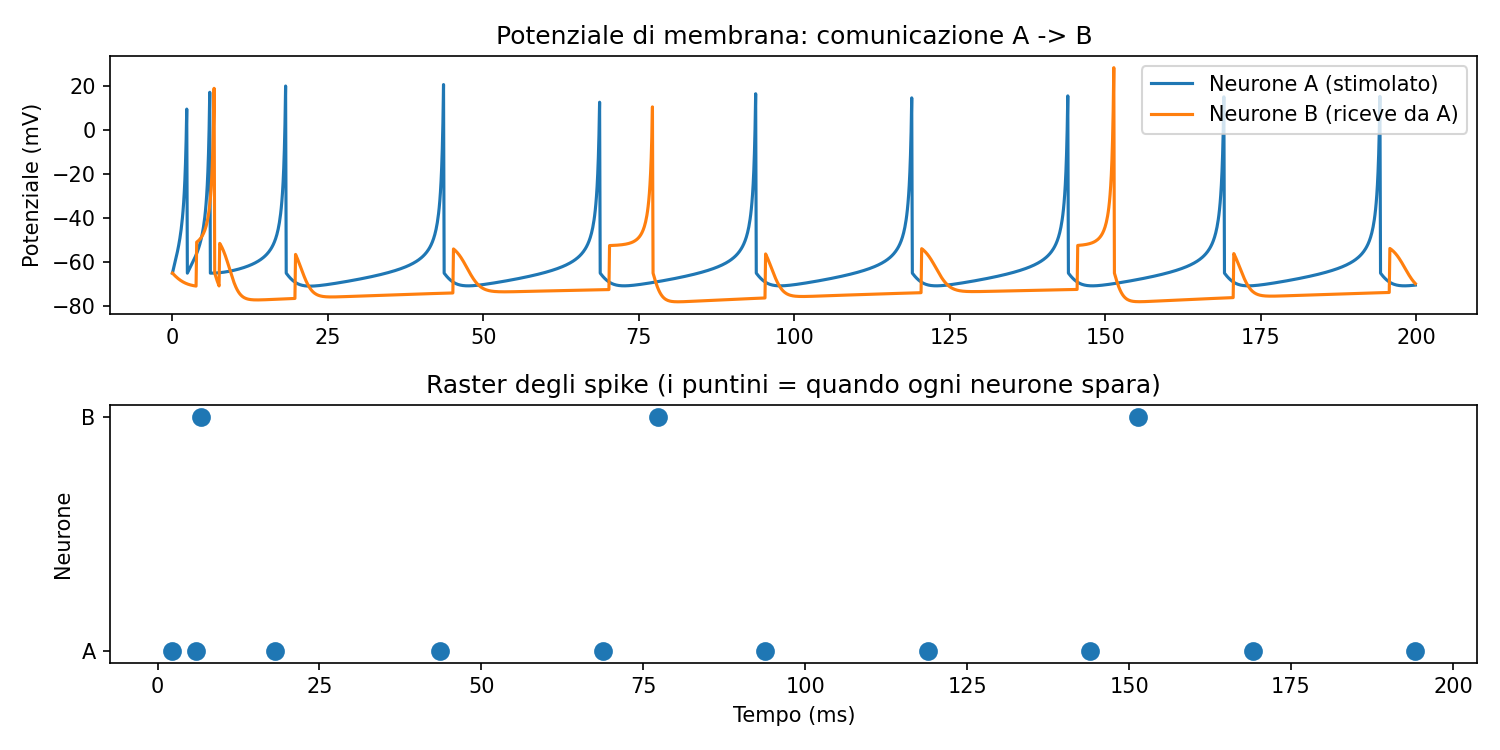
\includegraphics[width=5.8in,height=2.9in]{media/media/image1.png}

\emph{Fig. 1 --- Potenziale di membrana e raster: comunicazione A$\rightarrow$B.}

\textit{\textbf{Codice sorgente: due\_neuroni.py}}

\lstinputlisting[language=Python]{scripts/due_neuroni.py}
\subsection{2.2 Soglia sinaptica}\label{soglia-sinaptica}

Il secondo esperimento esplora sistematicamente un parametro che nel primo esperimento era fissato arbitrariamente: quanto deve essere forte una sinapsi perche\textquotesingle{} B risponda? Facendo variare l\textquotesingle intensita\textquotesingle{} della sinapsi tra 2 e 30 millivolt (mantenendo tutto il resto identico), si osserva una transizione netta e non lineare:

{\def\LTcaptype{none} % do not increment counter
\begin{longtable}[]{@{}
  >{\raggedright\arraybackslash}p{(\linewidth - 4\tabcolsep) * \real{0.3333}}
  >{\raggedright\arraybackslash}p{(\linewidth - 4\tabcolsep) * \real{0.3333}}
  >{\raggedright\arraybackslash}p{(\linewidth - 4\tabcolsep) * \real{0.3333}}@{}}
\toprule\noalign{}
\begin{minipage}[b]{\linewidth}\raggedright
\textbf{Intensita\textquotesingle{} sinapsi (mV)}
\end{minipage} & \begin{minipage}[b]{\linewidth}\raggedright
\textbf{Spike di A}
\end{minipage} & \begin{minipage}[b]{\linewidth}\raggedright
\textbf{Spike di B}
\end{minipage} \\
\midrule\noalign{}
\endhead
\bottomrule\noalign{}
\endlastfoot
2 & 10 & 0 \\
5 & 10 & 0 \\
10 & 10 & 0 \\
20 & 10 & 3 \\
30 & 10 & 7 \\
\end{longtable}
}

Sotto i 10-15 millivolt il neurone B non risponde mai, indipendentemente da quante volte A spari; sopra questa soglia, B risponde con una frequenza crescente in modo pressoche\textquotesingle{} monotono. Questo dimostra concretamente il concetto di soglia di attivazione -\/- un fenomeno intrinsecamente non lineare, non un semplice effetto proporzionale (raddoppiare l\textquotesingle intensita\textquotesingle{} della sinapsi da 5 a 10 mV non produce alcun cambiamento misurabile; raddoppiarla da 10 a 20 mV produce un cambiamento drastico, da zero risposta a risposta sostanziale).

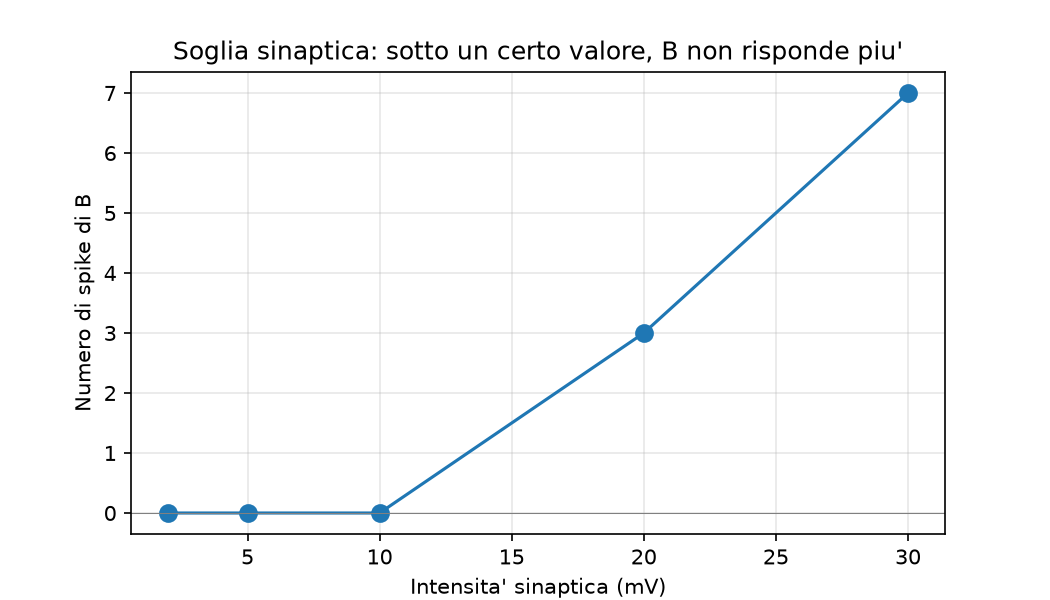
\includegraphics[width=4.5in,height=2.57143in]{media/media/image2.png}

\emph{Fig. 2 --- Soglia sinaptica: transizione netta tra 10 e 20 mV.}

\textit{\textbf{Codice sorgente: esplorazione\_parametri.py}}

\lstinputlisting[language=Python]{scripts/esplorazione_parametri.py}
\subsection{2.3 Plasticita\textquotesingle{} sinaptica a breve termine (facilitazione)}\label{plasticita-sinaptica-a-breve-termine-facilitazione}

Fino a questo punto, l\textquotesingle intensita\textquotesingle{} della sinapsi era un valore fisso, deciso una volta per tutte all\textquotesingle inizio della simulazione. Il terzo esperimento introduce il primo elemento di dinamica: una sinapsi la cui intensita\textquotesingle{} CAMBIA nel tempo in base a come viene usata -\/- il primo passo, per quanto elementare, verso il concetto di "storia" sinaptica.

Il meccanismo implementato si chiama facilitazione a breve termine (short-term facilitation): ogni volta che A genera uno spike, il peso della sinapsi verso B aumenta di un incremento fisso; tra uno spike e il successivo, il peso decade esponenzialmente verso un valore di base, con una costante di tempo di 50 millisecondi. Il risultato e\textquotesingle{} un peso sinaptico che, in presenza di spike ravvicinati nel tempo, sale progressivamente fino a raggiungere un equilibrio dinamico tra rafforzamento e decadimento -\/- un "dente di sega" visibile chiaramente nel grafico centrale della figura seguente.

Nell\textquotesingle arco della simulazione, A produce 17 spike e B risponde con 5 -\/- ma a differenza del secondo esperimento, i primi spike di A (quando il peso sinaptico e\textquotesingle{} ancora al valore base, sotto soglia) non fanno scattare B; solo dopo che il peso si e\textquotesingle{} rafforzato a sufficienza tramite ripetizione, B inizia a rispondere.

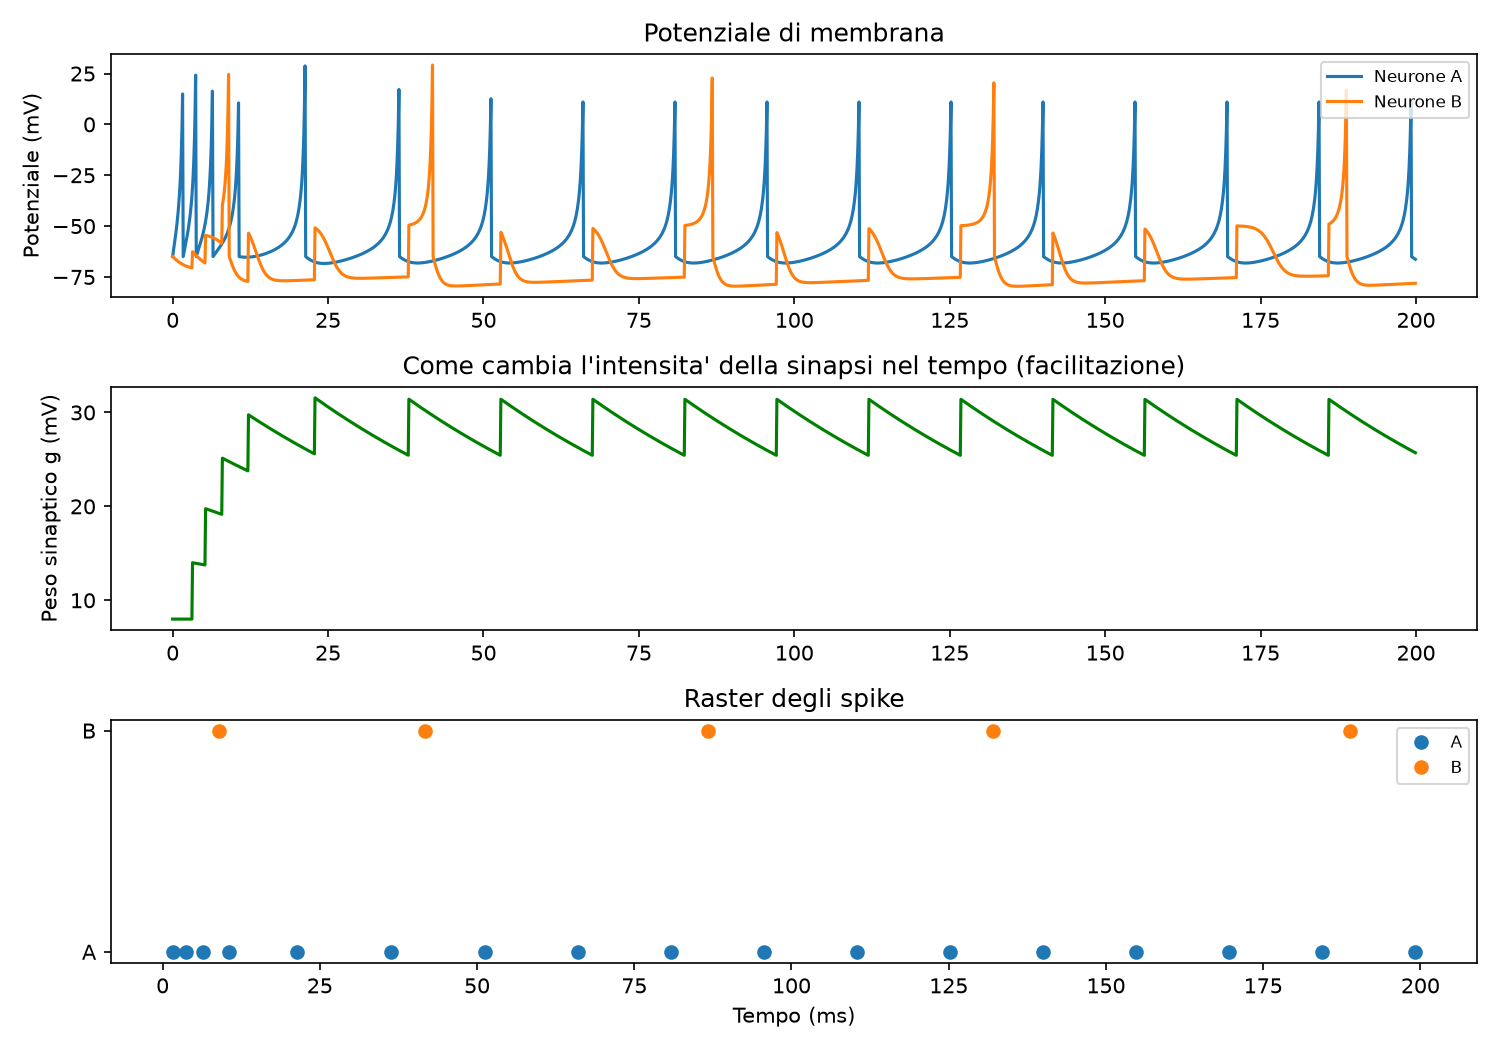
\includegraphics[width=5.8in,height=4.06in]{media/media/image3.png}

\emph{Fig. 3 --- Evoluzione del peso sinaptico con facilitazione a breve termine.}

\textit{\textbf{Codice sorgente: plasticita\_sinaptica.py}}

\lstinputlisting[language=Python]{scripts/plasticita_sinaptica.py}
\subsection{2.4 Propagazione in una catena di neuroni}\label{propagazione-in-una-catena-di-neuroni}

Il quarto esperimento passa da due neuroni a otto, collegati in sequenza lineare (N0$\rightarrow$N1$\rightarrow$N2$\rightarrow$...$\rightarrow$N7, ciascuno connesso solo al successivo). Solo N0 riceve uno stimolo esterno; il segnale deve attraversare l\textquotesingle intera catena tramite sinapsi identiche a quelle gia\textquotesingle{} verificate.

Il risultato principale e\textquotesingle{} la misura del ritardo di propagazione: ogni passaggio da un neurone al successivo introduce circa 3-4 millisecondi di ritardo (dovuto alla combinazione del delay sinaptico e del tempo di integrazione del neurone ricevente), per un ritardo totale accumulato di 25.9 millisecondi dal primo all\textquotesingle ultimo neurone della catena. Il raster della simulazione mostra tre "ondate" distinte e ben separate nel tempo, ciascuna corrispondente a una raffica di spike di N0 che si propaga in modo pulito lungo tutta la catena, con un pattern diagonale visibile a occhio nudo.

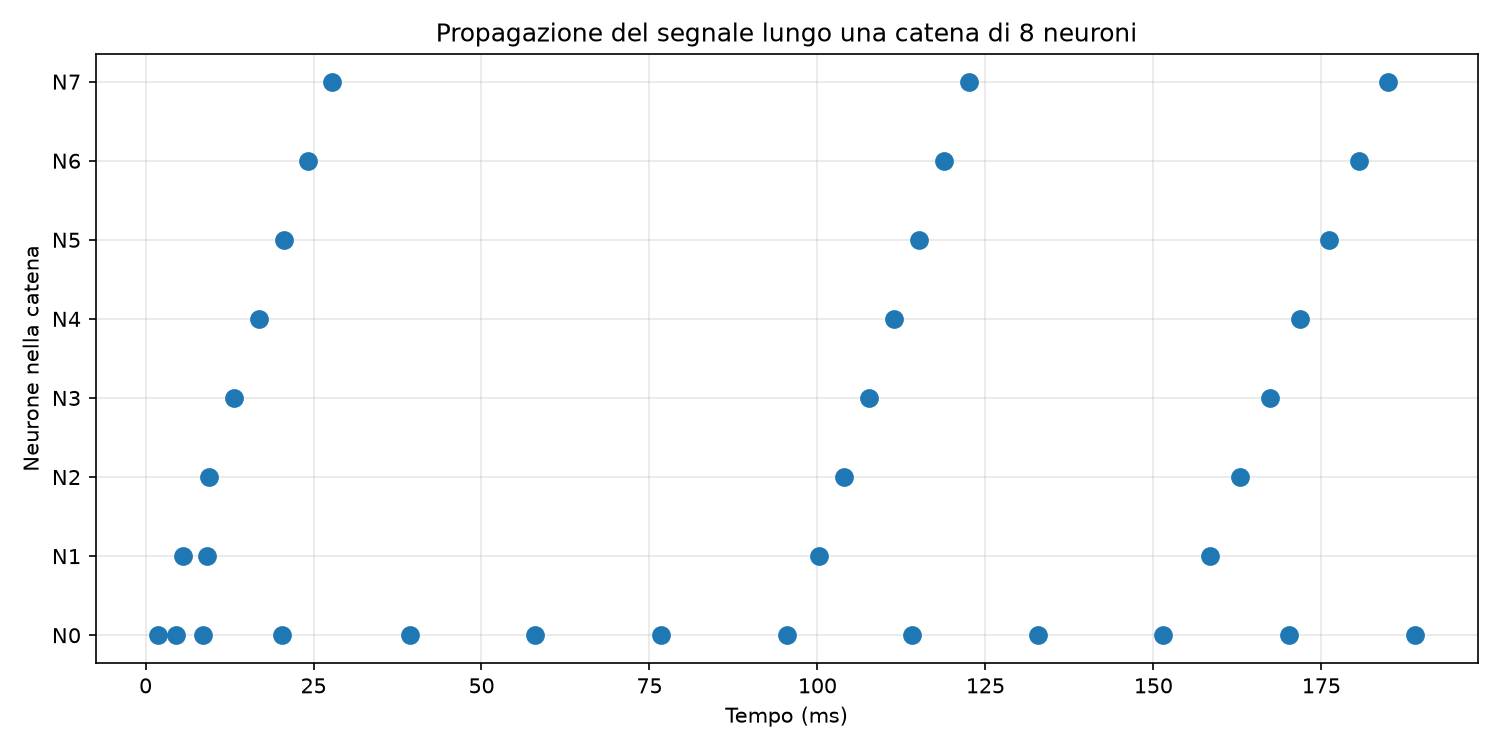
\includegraphics[width=5.8in,height=2.9in]{media/media/image4.png}

\emph{Fig. 4 --- Propagazione a onde lungo una catena di 8 neuroni.}

\textit{\textbf{Codice sorgente: rete\_catena.py}}

\lstinputlisting[language=Python]{scripts/rete_catena.py}
\subsection{2.5 Sommazione temporale (convergenza)}\label{sommazione-temporale-convergenza}

Il quinto esperimento inverte la topologia: invece di una catena lineare, tre neuroni indipendenti (N0, N1, N2) convergono su un quarto neurone bersaglio (N3). Ciascuno dei tre neuroni sorgente spara esattamente una volta, con la stessa identica intensita\textquotesingle{} sinaptica (10 mV) verso N3 in entrambi gli scenari testati.

Nello scenario "sincrono", i tre spike arrivano nello stesso istante (t=10ms): N3 riceve tutto l\textquotesingle input insieme, il potenziale sale di scatto e supera la soglia -\/- N3 spara. Nello scenario "sfasato", gli stessi tre spike arrivano distanziati di 5 millisecondi l\textquotesingle uno dall\textquotesingle altro (t=10, 15, 20ms): il potenziale di N3 sale a piccoli gradini ma decade tra un input e l\textquotesingle altro, non raggiungendo mai la soglia -\/- N3 non spara mai, nonostante abbia ricevuto esattamente la stessa quantita\textquotesingle{} totale di stimolazione.

Questo dimostra il principio di sommazione temporale, o "coincidence detection": un neurone non conta solo QUANTI input riceve, ma QUANTO SONO VICINI nel tempo. E\textquotesingle{} uno dei meccanismi computazionali piu\textquotesingle{} fondamentali con cui un singolo neurone puo\textquotesingle{} agire da rilevatore di correlazioni tra segnali in ingresso.

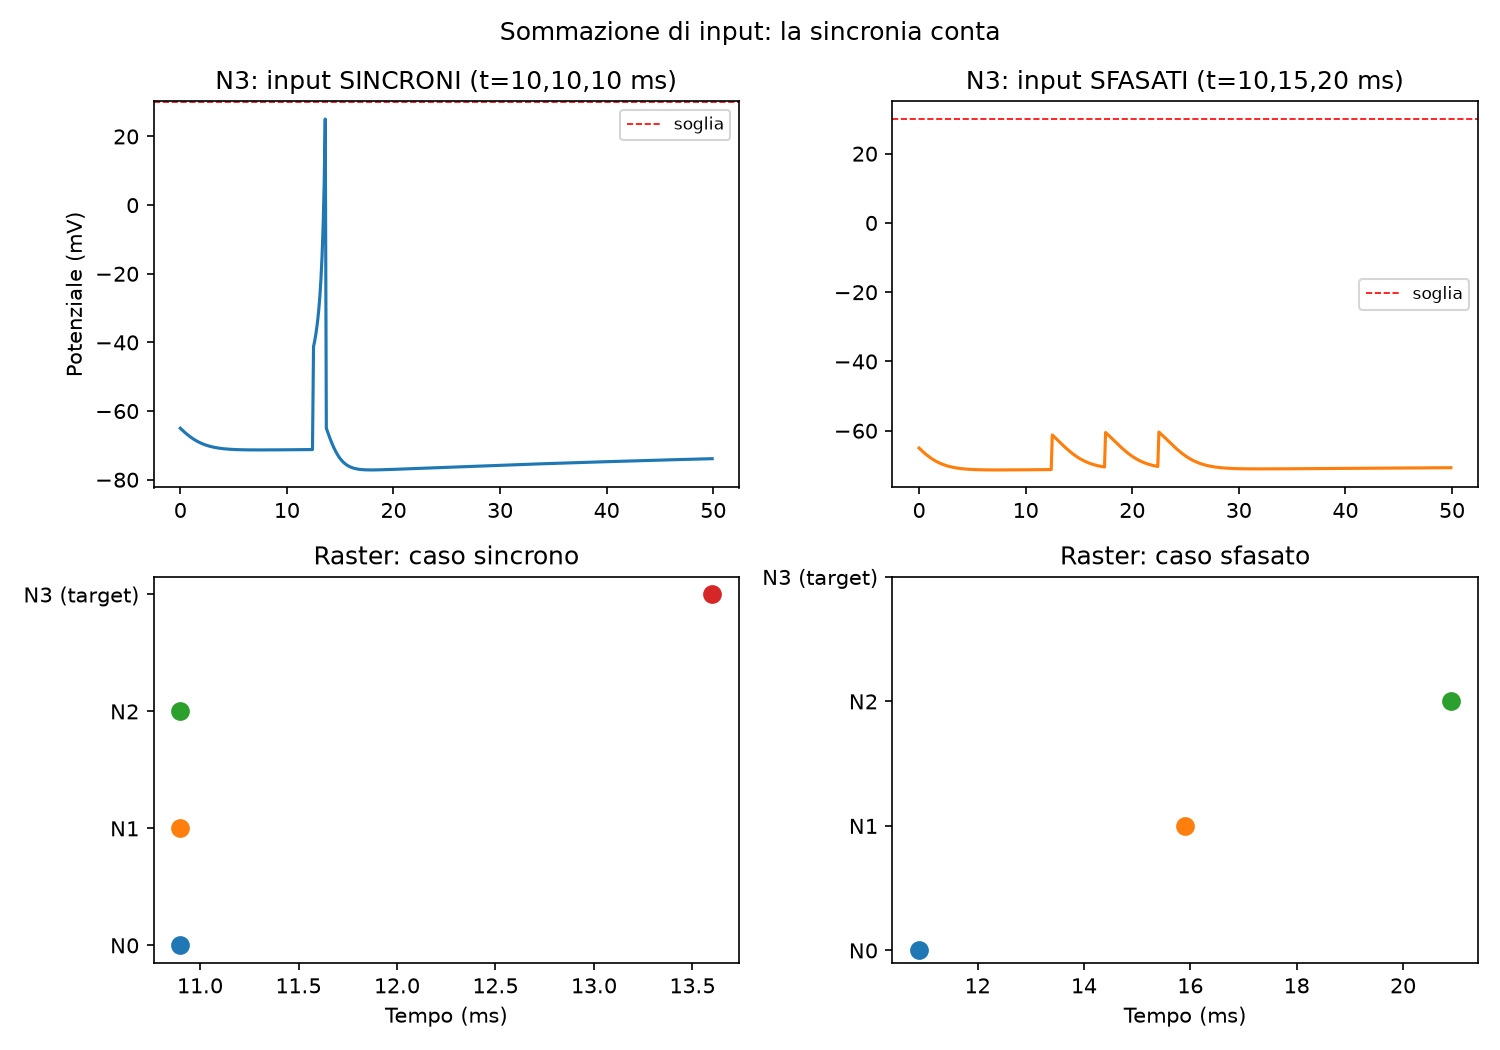
\includegraphics[width=5.8in,height=4.06in]{media/media/image5.png}

\emph{Fig. 5 --- Sommazione temporale: sincronia vs input sfasati.}

\textit{\textbf{Codice sorgente: rete\_convergente.py}}

\lstinputlisting[language=Python]{scripts/rete_convergente.py}
\subsection{2.6 STDP --- Spike-Timing-Dependent Plasticity}\label{stdp-spike-timing-dependent-plasticity}

Il sesto esperimento sostituisce la semplice facilitazione a breve termine (esperimento 2.3) con una regola di apprendimento molto piu\textquotesingle{} realistica e molto piu\textquotesingle{} usata nella letteratura di neuroscienza computazionale: la Spike-Timing-Dependent Plasticity (STDP), spesso riassunta con la formula mnemonica "i neuroni che sparano insieme si connettono insieme" (versione temporale della regola di Hebb, 1949).

Il principio: se il neurone presinaptico (A) spara sistematicamente POCO PRIMA del neurone postsinaptico (B), la sinapsi A$\rightarrow$B si RAFFORZA (potenziamento, LTP - Long-Term Potentiation), perche\textquotesingle{} A sembra "predire" B, una relazione potenzialmente causale. Se invece A spara POCO DOPO B, la sinapsi si INDEBOLISCE (depressione, LTD). L\textquotesingle implementazione in Brian2 usa due variabili di traccia esponenziale (apre, apost) che si accumulano ad ogni spike e decadono con costante di tempo di 20 millisecondi -\/- il meccanismo standard per implementare STDP in modo efficiente senza dover confrontare esplicitamente ogni coppia di spike passati.

Verificato su 5 ripetizioni di un pattern fisso "A spara 5 millisecondi prima di B": il peso sinaptico sale in modo monotono e a scalini, da un valore iniziale di 5.00 mV fino a 8.36 mV dopo le 5 ripetizioni -\/- un rafforzamento netto di 3.36 mV attribuibile interamente alla regola STDP.

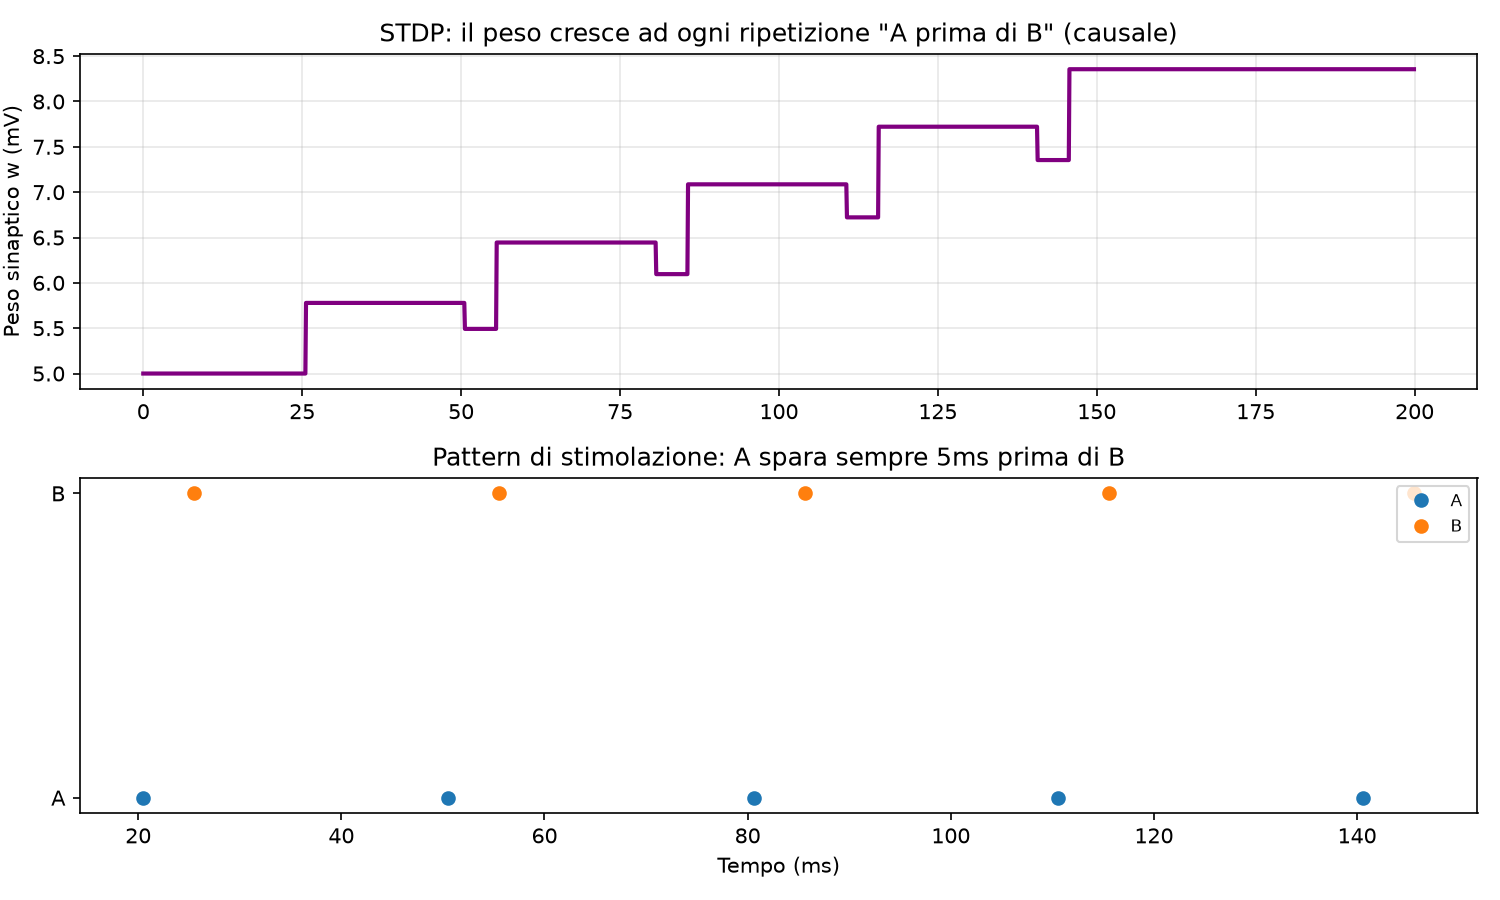
\includegraphics[width=5.5in,height=3.3in]{media/media/image6.png}

\emph{Fig. 6 --- Rafforzamento del peso sinaptico via STDP su ripetizioni causali.}

\textit{\textbf{Codice sorgente: stdp.py}}

\lstinputlisting[language=Python]{scripts/stdp.py}
\subsection{2.7 Classificazione di pattern tramite STDP}\label{classificazione-di-pattern-tramite-stdp}

Il settimo esperimento e\textquotesingle{} il primo salto concettuale importante del progetto: non piu\textquotesingle{} solo osservare come cambia UN peso sinaptico, ma verificare se un intero piccolo circuito puo\textquotesingle{} IMPARARE a distinguere due pattern di input diversi, senza che nessuno gli scriva esplicitamente la regola di distinzione.

Struttura: 6 neuroni di input, divisi in due gruppi di 3 (Gruppo A e Gruppo B, che rappresentano due "pattern" distinti). Un neurone di output O riceve da tutti e 6 tramite sinapsi plastiche STDP, con pesi iniziali tutti uguali e bassi (6 mV). Durante il training (10 ripetizioni), ogni volta che viene presentato il Pattern A, un piccolo "maestro" esterno forza O a sparare subito dopo -\/- come un insegnante che guida la risposta corretta. Quando viene presentato il Pattern B, nessun aiuto esterno e\textquotesingle{} fornito.

Nella fase di TEST, senza alcun aiuto esterno: il Pattern A presentato da solo fa sparare O; il Pattern B presentato da solo NON lo fa sparare. I pesi finali confermano il meccanismo: le sinapsi del Gruppo A sono salite fino a saturare al valore massimo consentito (15.00 mV), mentre quelle del Gruppo B sono rimaste vicine al valore iniziale, anzi leggermente indebolite (5.67 mV). Il comportamento discriminativo -\/- rispondere selettivamente a un pattern e non all\textquotesingle altro -\/- e\textquotesingle{} EMERSO dalla regola STDP applicata ripetutamente, non e\textquotesingle{} stato scritto esplicitamente da nessuna parte nel codice come una condizione "if pattern == A".

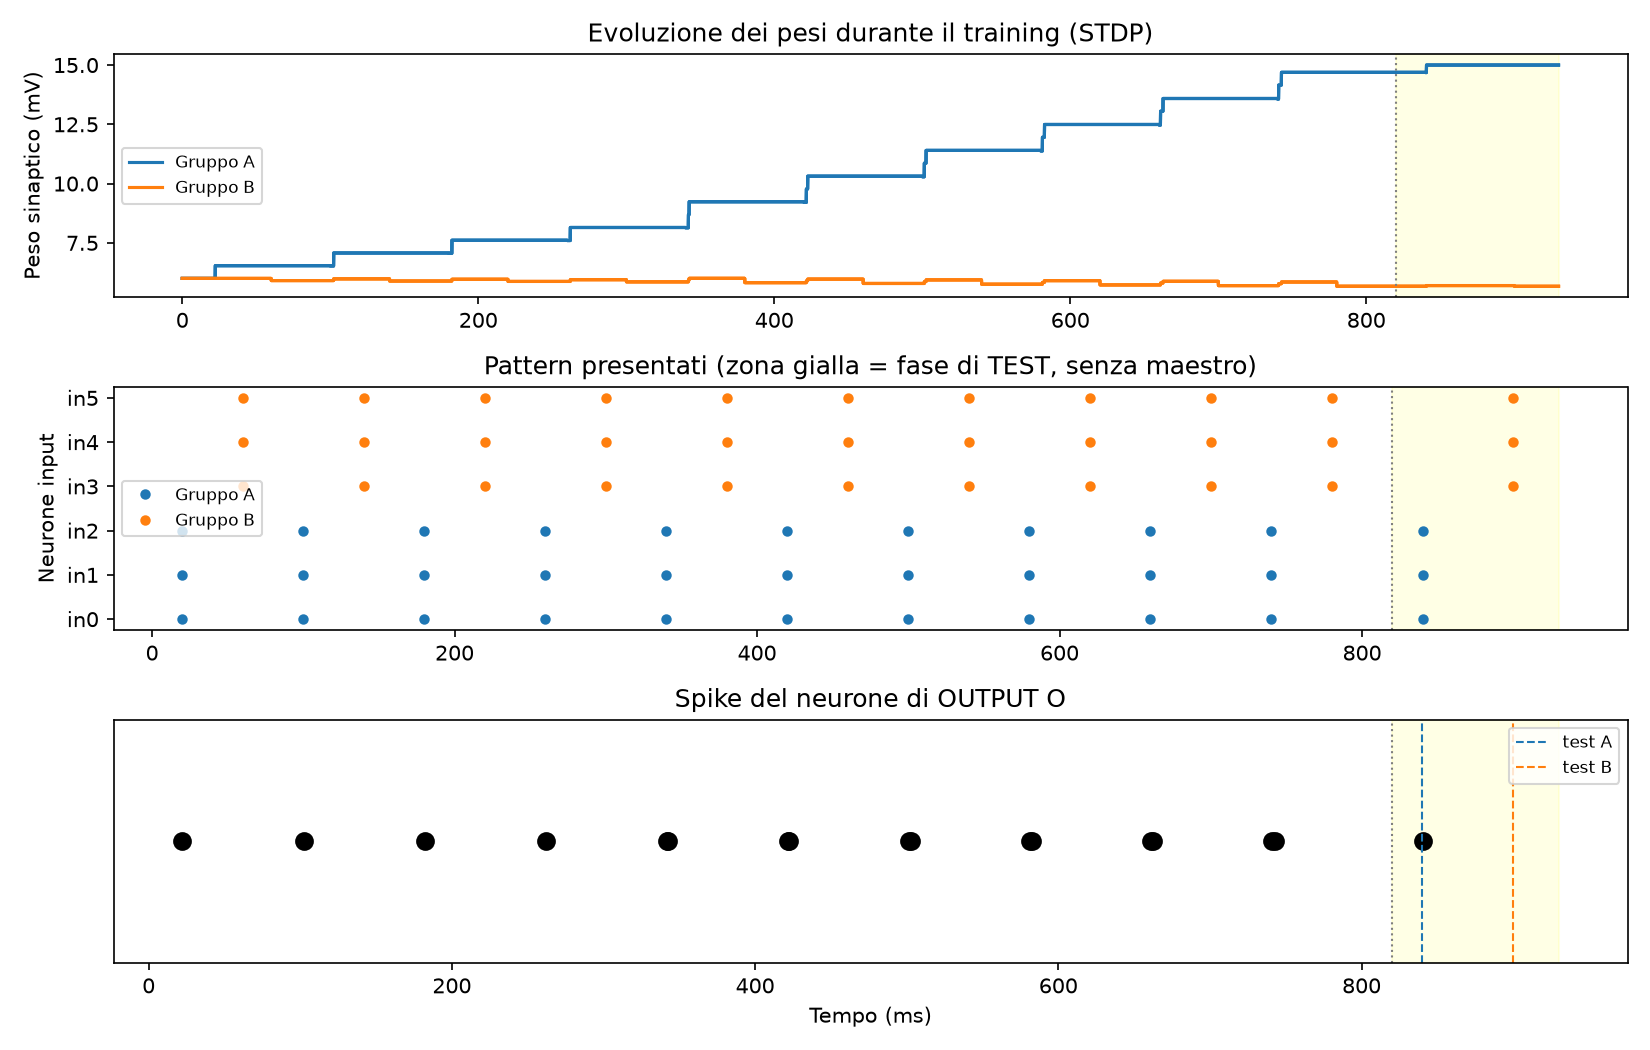
\includegraphics[width=5.8in,height=3.69091in]{media/media/image7.png}

\emph{Fig. 7 --- Apprendimento selettivo: risposta solo al Pattern A dopo training.}

\textit{\textbf{Codice sorgente: classificazione\_stdp.py}}

\lstinputlisting[language=Python]{scripts/classificazione_stdp.py}
\subsection{2.8 Rete bilanciata eccitazione-inibizione (300 neuroni)}\label{rete-bilanciata-eccitazione-inibizione-300-neuroni}

L\textquotesingle ottavo esperimento e\textquotesingle{} il primo salto di scala reale del progetto: da poche unita\textquotesingle{} di neuroni a 300, organizzati secondo l\textquotesingle architettura standard della letteratura di neuroscienza computazionale per reti di questa dimensione -\/- il modello "bilanciato" ispirato ai lavori di Nicolas Brunel (2000).

La rete e\textquotesingle{} composta da 240 neuroni eccitatori (80\%, che spingono i neuroni bersaglio verso lo spike) e 60 neuroni inibitori (20\%, che sopprimono l\textquotesingle attivita\textquotesingle), con connettivita\textquotesingle{} sparsa e casuale al 10\% (ogni coppia di neuroni ha il 10\% di probabilita\textquotesingle{} di essere connessa, indipendentemente dalle altre coppie). Un tentativo preliminare con sole sinapsi eccitatorie (non mostrato nel dettaglio in questo documento, ma verificato durante lo sviluppo) porta la rete a esplodere in una scarica sincronizzata di tutta la popolazione, oppure a spegnersi del tutto -\/- nessuno dei due comportamenti e\textquotesingle{} interessante o realistico.

Introducendo l\textquotesingle inibizione nella proporzione corretta, si ottiene invece uno stato di attivita\textquotesingle{} detto "asincrona irregolare": i neuroni sparano a una frequenza media di circa 15.6 Hz, in modo statisticamente strutturato ma senza sincronizzarsi tutti insieme -\/- qualitativamente simile all\textquotesingle attivita\textquotesingle{} osservata nella corteccia cerebrale reale durante la veglia.

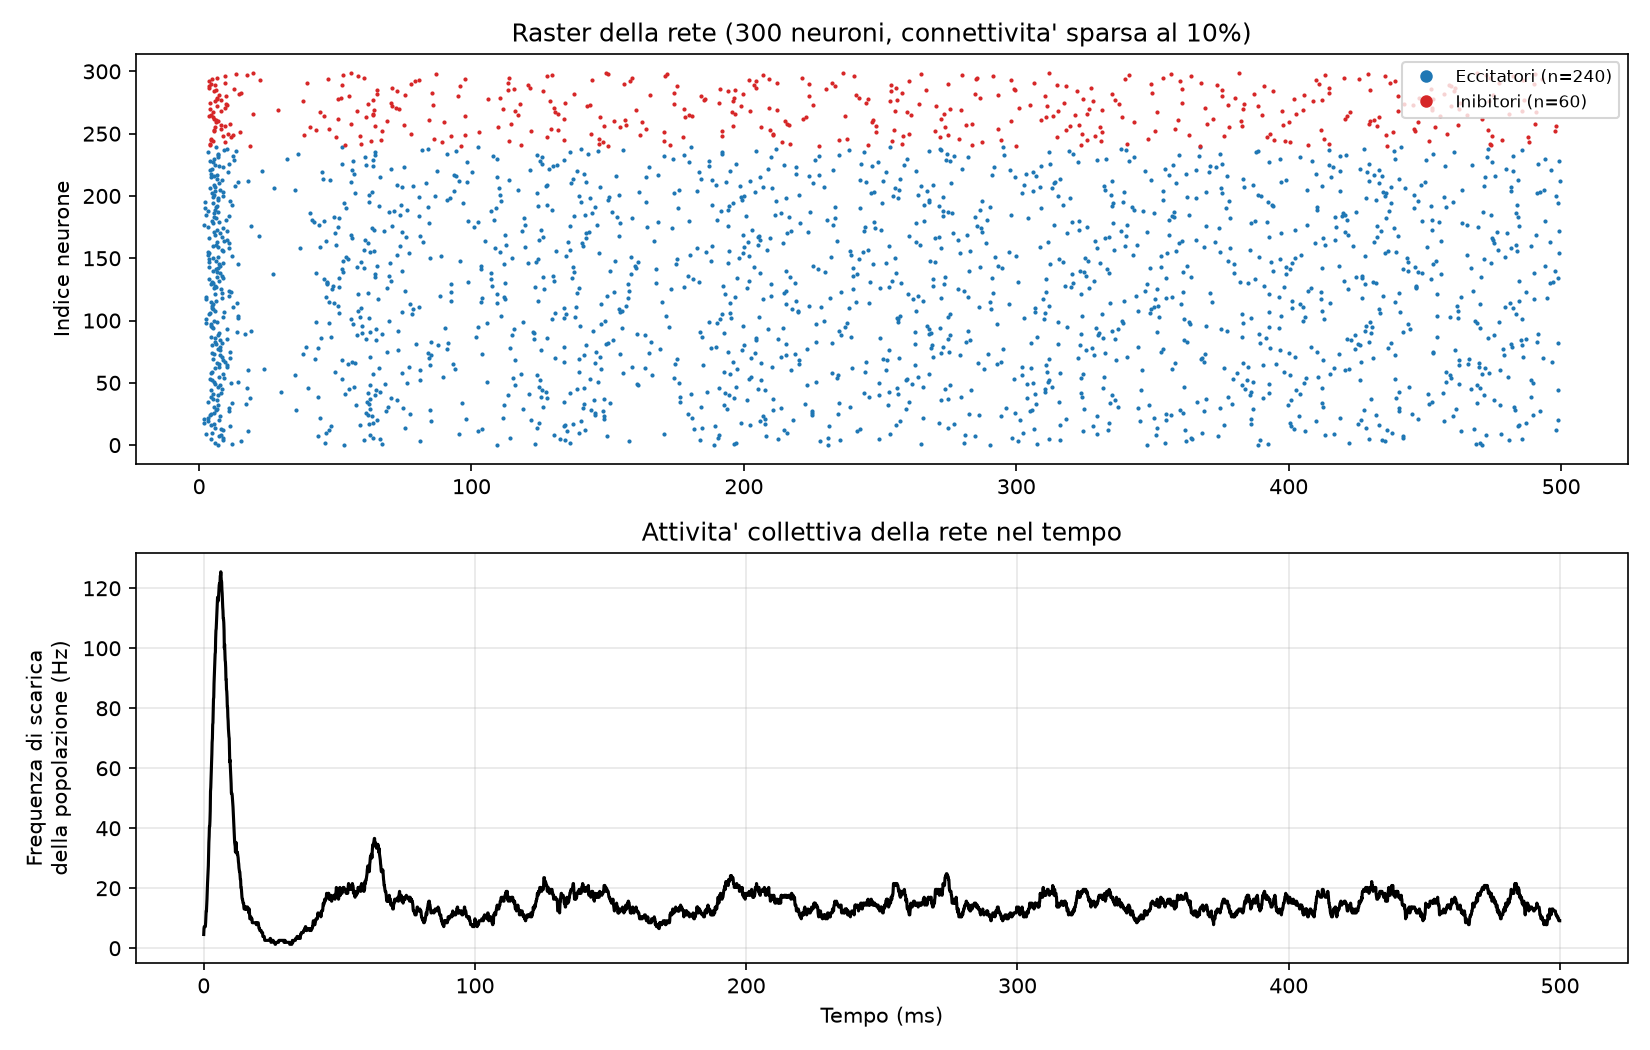
\includegraphics[width=5.8in,height=3.69091in]{media/media/image8.png}

\emph{Fig. 8 --- Raster e frequenza collettiva della rete a 300 neuroni.}

\textit{\textbf{Codice sorgente: rete\_300\_neuroni.py}}

\lstinputlisting[language=Python]{scripts/rete_300_neuroni.py}
\subsection{2.9 Risposta a uno stimolo e recupero omeostatico}\label{risposta-a-uno-stimolo-e-recupero-omeostatico}

Il nono esperimento verifica come la rete a 300 neuroni, gia\textquotesingle{} stabile nel suo stato di attivita\textquotesingle{} spontanea, risponde a una perturbazione esterna. Si applica un impulso di corrente forte a soli 20 neuroni su 300 (il 6.7\% della rete) per 20 millisecondi, poi lo si rimuove completamente.

La frequenza collettiva della rete sale bruscamente da circa 14.9 Hz (baseline) a un picco di circa 68.6 Hz durante e subito dopo lo stimolo, per poi tornare spontaneamente al livello di partenza (15.6 Hz) senza alcun intervento esterno. Un dettaglio interessante, visibile chiaramente nel grafico: dopo il picco, la frequenza non torna dolcemente alla baseline ma scende brevemente SOTTO il livello di partenza (un "undershoot" inibitorio) prima di ristabilizzarsi -\/- un comportamento tipico dei sistemi con feedback negativo, dove i neuroni inibitori attivati dall\textquotesingle ondata eccitatoria restano attivi un istante piu\textquotesingle{} a lungo del necessario.

Questo comportamento -\/- risposta proporzionata a uno stimolo, seguita da un ritorno spontaneo all\textquotesingle equilibrio -\/- e\textquotesingle{} la prima comparsa nel progetto di qualcosa che assomiglia a OMEOSTASI, una proprieta\textquotesingle{} fondamentale di qualunque sistema nervoso funzionante: la capacita\textquotesingle{} di rispondere senza restare "danneggiato" o entrare in un regime patologico.

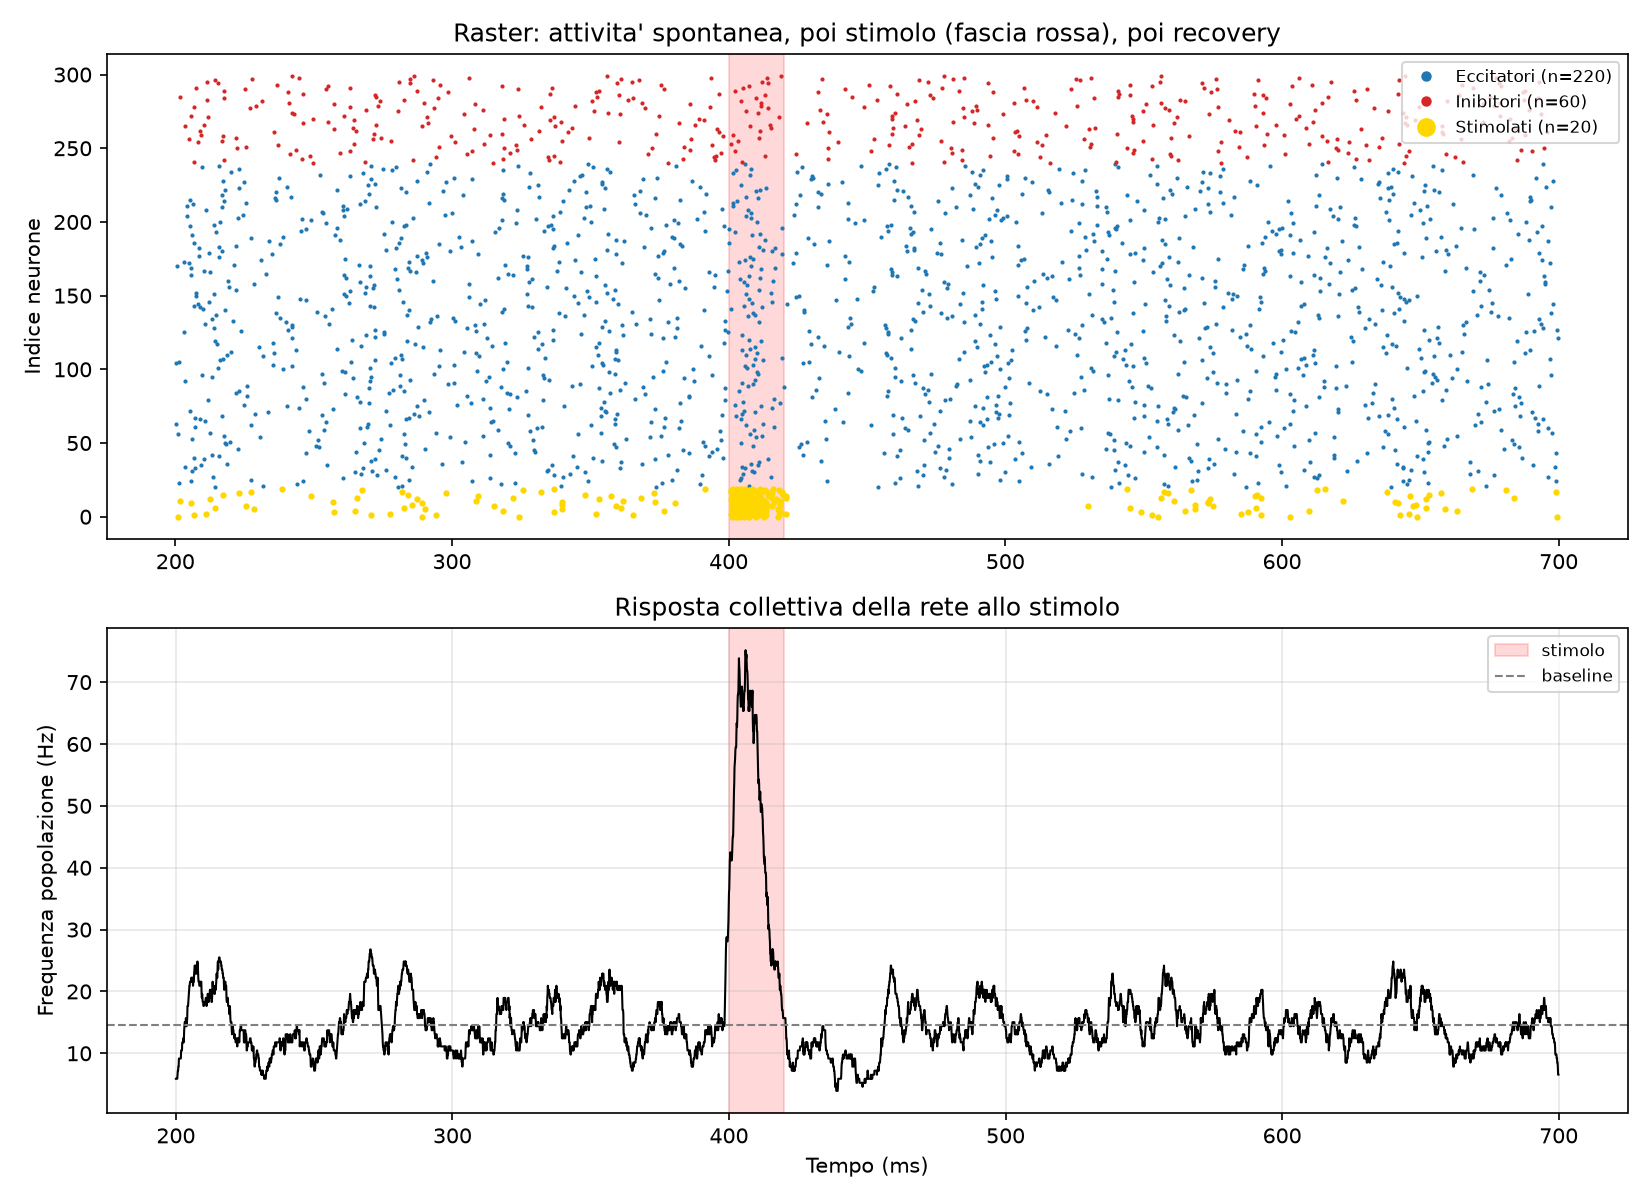
\includegraphics[width=5.8in,height=4.21818in]{media/media/image9.png}

\emph{Fig. 9 --- Risposta e recupero omeostatico dopo stimolo mirato.}

\textit{\textbf{Codice sorgente: rete\_300\_stimolo.py}}

\lstinputlisting[language=Python]{scripts/rete_300_stimolo.py}
\subsection{2.10 Architettura modulare: due regioni collegate}\label{architettura-modulare-due-regioni-collegate}

Il decimo esperimento introduce per la prima volta nel progetto il concetto di REGIONI distinte, anziche\textquotesingle{} un\textquotesingle unica massa di neuroni indifferenziata. La rete a 300 neuroni viene divisa in due moduli da 150 ciascuno (identica struttura E/I interna, connettivita\textquotesingle{} densa al 10\% come prima), ma collegati tra loro solo debolmente: 2\% di probabilita\textquotesingle{} di connessione, e SOLO sinapsi eccitatorie -\/- una scelta che rispecchia come funzionano davvero le connessioni cortico-corticali a lungo raggio nel cervello reale, tipicamente eccitatorie e relativamente sparse rispetto alla densita\textquotesingle{} di connessione all\textquotesingle interno di una singola area.

Stimolando SOLO il Modulo 1 (20 neuroni, come nell\textquotesingle esperimento 2.9), si osserva in una singola prova un apparente aumento di attivita\textquotesingle{} anche nel Modulo 2, che non ha ricevuto alcuno stimolo diretto: +88 Hz nel Modulo 1 (stimolato direttamente) e +13 Hz nel Modulo 2 (attenuato ma presente, apparentemente). A prima vista, questo sembrerebbe dimostrare che il segnale si propaga tra le due regioni tramite le poche connessioni che le collegano.

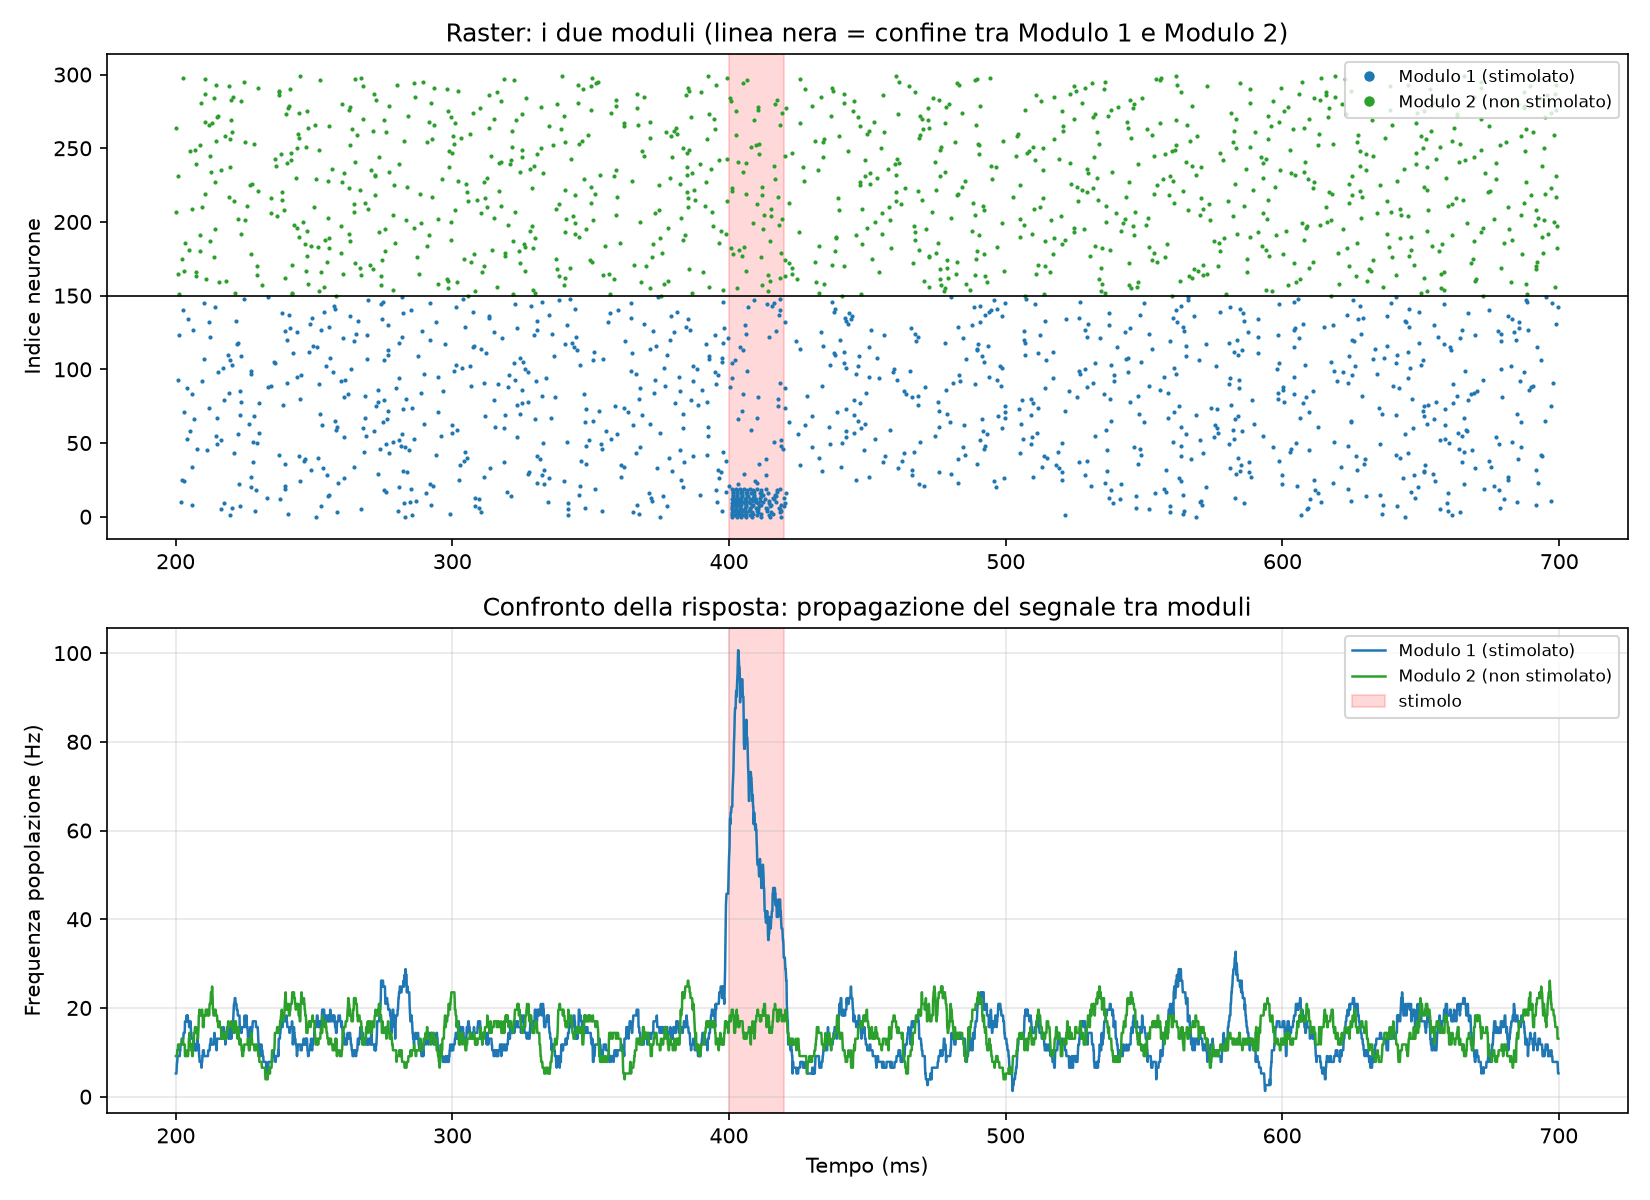
\includegraphics[width=5.8in,height=4.21818in]{media/media/image10.png}

\emph{Fig. 10 --- Propagazione apparente tra moduli (singola prova).}

\textit{\textbf{Codice sorgente: due\_moduli.py}}

\lstinputlisting[language=Python]{scripts/due_moduli.py}
\subsection{2.11 Verifica statistica: l\textquotesingle effetto osservato e\textquotesingle{} reale o rumore?}\label{verifica-statistica-leffetto-osservato-e-reale-o-rumore}

\textbf{L\textquotesingle undicesimo esperimento e\textquotesingle, dal punto di vista metodologico, probabilmente il piu\textquotesingle{} importante dell\textquotesingle intero progetto -\/- non per il risultato positivo che produce, ma per quello che INSEGNA sul rigore scientifico necessario prima di trarre conclusioni.}

Osservando con attenzione il grafico dell\textquotesingle esperimento 2.10, il piccolo aumento di attivita\textquotesingle{} nel Modulo 2 (+13 Hz) risultava paragonabile in ampiezza alle normali fluttuazioni spontanee della rete, visibili in altri punti dello stesso grafico anche senza alcuno stimolo in corso. Una singola prova non permette di distinguere un vero effetto di propagazione da una coincidenza statistica.

La soluzione adottata e\textquotesingle{} la tecnica standard usata in neuroscienza sperimentale per questo esatto problema: il PSTH (Peristimulus Time Histogram). Si ripete l\textquotesingle esperimento identico 25 volte, si allinea ogni prova rispetto al momento esatto dello stimolo, e si calcola la MEDIA su tutte le prove -\/- se esiste un vero effetto, nella media emerge chiaramente sopra il rumore (che tende a cancellarsi mediando su molte ripetizioni indipendenti); se non esiste alcun vero effetto, la media resta piatta.

Risultato della verifica: l\textquotesingle effetto medio misurato sul Modulo 2, mediato su 25 ripetizioni, e\textquotesingle{} risultato di appena +0.89 Hz -\/- chiaramente dentro il rumore di fondo (la deviazione standard di una singola prova, misurata sulla stessa finestra temporale, e\textquotesingle{} di circa 4 Hz, quasi 5 volte piu\textquotesingle{} grande dell\textquotesingle effetto medio osservato).

\textbf{Conclusione onesta: con questi parametri di connettivita\textquotesingle{} (2\% di probabilita\textquotesingle, solo sinapsi eccitatorie), NON e\textquotesingle{} possibile affermare con sicurezza che il segnale si propaghi in modo significativo tra i due moduli. Quello che sembrava un effetto chiaro nella singola prova era, con ogni probabilita\textquotesingle, in gran parte rumore statistico casuale.}

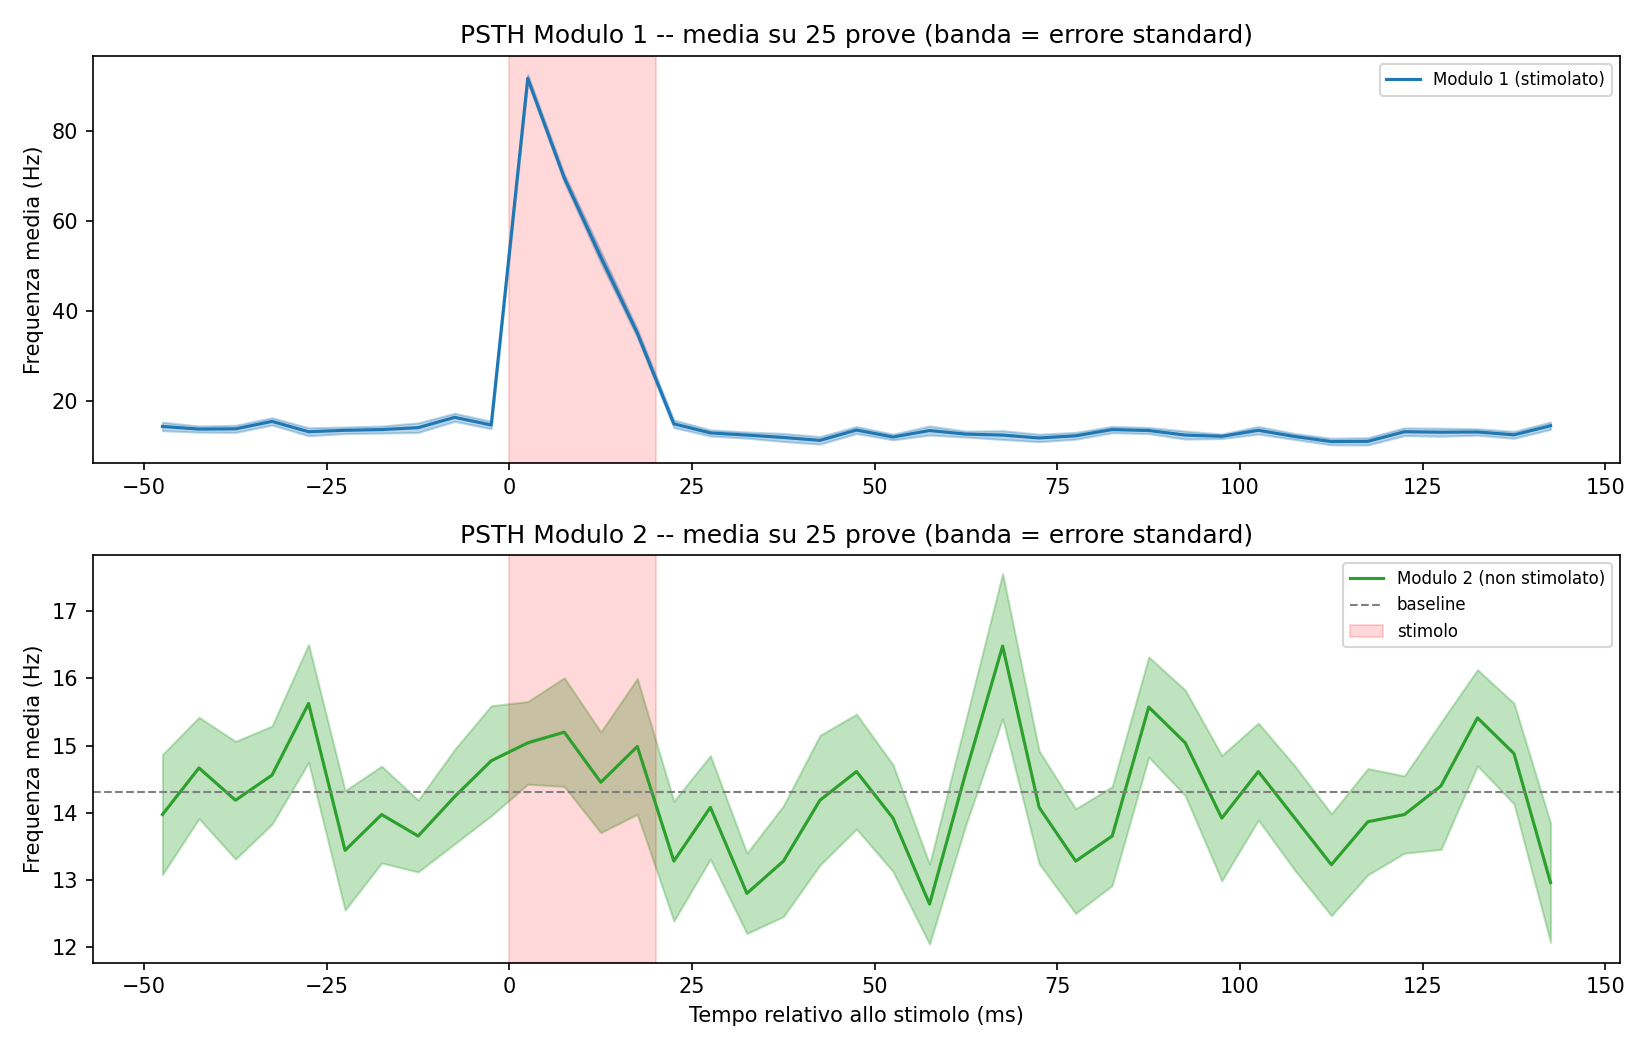
\includegraphics[width=5.8in,height=3.69091in]{media/media/image11.png}

\emph{Fig. 11 --- PSTH su 25 prove: l\textquotesingle effetto medio rientra nel rumore.}

Questo risultato negativo, ottenuto con lo strumento statistico corretto, e\textquotesingle{} probabilmente il contributo piu\textquotesingle{} solido dell\textquotesingle intero progetto dal punto di vista del metodo scientifico: mostra la differenza concreta tra un risultato che SEMBRA interessante a un primo sguardo e un risultato VERIFICATO con gli strumenti statistici adeguati -\/- una distinzione che ricorre, sotto forme diverse, anche piu\textquotesingle{} avanti nel documento (sezione 4.2, sezione 5.3).

\textit{\textbf{Codice sorgente: psth\_moduli.py}}

\lstinputlisting[language=Python]{scripts/psth_moduli.py}
\section{3. Scaling verso la dimensione di un cervello di topo}\label{scaling-verso-la-dimensione-di-un-cervello-di-topo}

\subsection{3.1 Il numero di riferimento e il vincolo di memoria}\label{il-numero-di-riferimento-e-il-vincolo-di-memoria}

Un cervello di topo ha circa 70 milioni di neuroni, contando l\textquotesingle intero encefalo (cervelletto incluso). Simularlo per intero con dettaglio biofisico paragonabile a quello usato in questo progetto e\textquotesingle{} oltre le possibilita\textquotesingle{} di un singolo laptop -\/- ma e\textquotesingle{} stato possibile misurare, passo dopo passo e con dati reali (non stimati a tavolino), quanto ci si potesse avvicinare realisticamente con l\textquotesingle hardware disponibile: un MacBook Air M5 con 24 GB di RAM totali.

Il vincolo dominante, come i dati di questa sezione dimostrano chiaramente, e\textquotesingle{} risultato essere la memoria RAM disponibile, non la velocita\textquotesingle{} di calcolo pura -\/- una scoperta empirica interessante di per se\textquotesingle, dato che inizialmente si sarebbe potuto aspettare il contrario.

\subsection{3.2 Il cambiamento tecnico chiave: connettivita\textquotesingle{} a grado fisso}\label{il-cambiamento-tecnico-chiave-connettivita-a-grado-fisso}

Per scalare oltre poche migliaia di neuroni, si e\textquotesingle{} dovuto abbandonare la sintassi standard di Brian2 per la connettivita\textquotesingle{} probabilistica. Il motivo e\textquotesingle{} puramente computazionale: la sintassi connect(condition=..., p=...) valuta, concettualmente, la probabilita\textquotesingle{} di connessione per OGNI possibile coppia di neuroni nella rete -\/- un costo che cresce come il quadrato del numero di neuroni (N\textsuperscript{2}). Per una rete di 40 milioni di neuroni, N\textsuperscript{2} sarebbe dell\textquotesingle ordine di 1.6 x 10\textsuperscript{1}\textsuperscript{5} -\/- un numero completamente impraticabile da processare, anche solo per generare la lista delle sinapsi, indipendentemente da quanto tempo si sarebbe disposti ad aspettare.

La soluzione adottata e\textquotesingle{} la connettivita\textquotesingle{} a GRADO FISSO: invece di una probabilita\textquotesingle{} di connessione valutata su tutte le coppie possibili, ogni neurone si connette a esattamente K altri neuroni (K=15 in questo progetto), scelti casualmente tra tutti i neuroni della rete. Il numero totale di sinapsi cresce cosi\textquotesingle{} in modo LINEARE con N (circa K$\times$N sinapsi totali per tipo di connessione), non quadratico -\/- ed e\textquotesingle{} proprio questa differenza, tra crescita lineare e quadratica, che rende possibile scalare a milioni di neuroni invece di restare bloccati a poche migliaia.

\emph{Connettivita\textquotesingle{} a probabilita\textquotesingle{} fissa: N\_sinapsi $\approx$ p $\times$ N\textsuperscript{2} (impraticabile oltre N\textasciitilde10\textsuperscript{4})}

\emph{Connettivita\textquotesingle{} a grado fisso: N\_sinapsi $\approx$ K $\times$ N (praticabile fino a N\textasciitilde10\textsuperscript{7}-10\textsuperscript{8})}

\subsection{3.3 Dati di scaling, misurati sul MacBook Air M5}\label{dati-di-scaling-misurati-sul-macbook-air-m5}

La tabella seguente riporta TUTTI i punti dati raccolti durante la fase di scaling, misurati direttamente sul MacBook Air M5 dell\textquotesingle autore attraverso quattro sessioni successive di test ("fase 1" fino a "fase 4"), ciascuna delle quali ha spinto la dimensione della rete un po\textquotesingle{} piu\textquotesingle{} in alto rispetto alla precedente, ricalibrando ogni volta la stima predittiva di memoria necessaria sui dati reali gia\textquotesingle{} raccolti (anziche\textquotesingle{} su un modello puramente teorico), per evitare di rischiare un crash del sistema per esaurimento di RAM.

{\def\LTcaptype{none} % do not increment counter
\begin{longtable}[]{@{}
  >{\raggedright\arraybackslash}p{(\linewidth - 8\tabcolsep) * \real{0.2000}}
  >{\raggedright\arraybackslash}p{(\linewidth - 8\tabcolsep) * \real{0.2000}}
  >{\raggedright\arraybackslash}p{(\linewidth - 8\tabcolsep) * \real{0.2000}}
  >{\raggedright\arraybackslash}p{(\linewidth - 8\tabcolsep) * \real{0.2000}}
  >{\raggedright\arraybackslash}p{(\linewidth - 8\tabcolsep) * \real{0.2000}}@{}}
\toprule\noalign{}
\begin{minipage}[b]{\linewidth}\raggedright
\textbf{N neuroni}
\end{minipage} & \begin{minipage}[b]{\linewidth}\raggedright
\textbf{N sinapsi}
\end{minipage} & \begin{minipage}[b]{\linewidth}\raggedright
\textbf{Tempo (s)}
\end{minipage} & \begin{minipage}[b]{\linewidth}\raggedright
\textbf{RAM (MB)}
\end{minipage} & \begin{minipage}[b]{\linewidth}\raggedright
\textbf{\% cervello di topo}
\end{minipage} \\
\midrule\noalign{}
\endhead
\bottomrule\noalign{}
\endlastfoot
1.000 & 31.000 & 1.12 & 301 & 0.001\% \\
10.000 & 310.000 & 9.04 & 330 & 0.014\% \\
100.000 & 3.100.000 & 1.37 & 444 & 0.143\% \\
500.000 & 15.500.000 & 6.44 & 873 & 0.714\% \\
1.000.000 & 31.000.000 & 12.91 & 1.720 & 1.429\% \\
3.000.000 & 93.000.000 & 38.85 & 4.152 & 4.286\% \\
5.000.000 & 155.000.000 & 65.66 & 6.254 & 7.143\% \\
10.000.000 & 310.000.000 & 133.28 & 9.838 & 14.286\% \\
20.000.000 & 620.000.000 & 269.71 & 11.147 & 28.571\% \\
25.000.000 & 775.000.000 & 336.75 & 11.495 & 35.714\% \\
30.000.000 & 930.000.000 & 405.57 & 12.434 & 42.857\% \\
35.000.000 & 1.085.000.000 & 497.05 & 15.104 & 50.000\% \\
40.000.000 & 1.240.000.000 & 573.08 & 15.744 & 57.143\% \\
\end{longtable}
}

A 50 milioni di neuroni (stima predittiva \textasciitilde21-25 GB di RAM), il tentativo e\textquotesingle{} stato interrotto dopo oltre un\textquotesingle ora senza completare nemmeno 200 millisecondi di tempo simulato. L\textquotesingle analisi tramite Monitoraggio Attivita\textquotesingle{} di macOS ha rivelato la causa: non un crash imminente, ma una fortissima compressione di memoria da parte del sistema operativo (visibile come pressione di memoria in stato "giallo", non "rosso" critico), che manteneva la CPU impegnata (77-95\% di utilizzo) senza pero\textquotesingle{} far avanzare il calcolo effettivo in modo proporzionale -\/- il classico segno di un sistema che sta spendendo la maggior parte del proprio tempo a comprimere e decomprimere dati in memoria invece di eseguire il calcolo richiesto. Il tentativo e\textquotesingle{} stato interrotto manualmente per prudenza.

\textbf{Il limite pratico verificato e completato con pieno successo resta quindi 40 milioni di neuroni -\/- il 57.1\% della scala di un cervello di topo.}

\subsection{3.4 Effetto del throttling termico}\label{effetto-del-throttling-termico}

Un fenomeno osservato solo nell\textquotesingle esperimento finale piu\textquotesingle{} esteso (sezione 3.6, con piu\textquotesingle{} fasi simulate in sequenza e una durata totale nettamente maggiore rispetto ai singoli benchmark di scaling): il MacBook Air, essendo un modello privo di ventola di raffreddamento attiva, rallenta progressivamente le proprie prestazioni sotto carico computazionale sostenuto per proteggersi dal surriscaldamento -\/- un comportamento protettivo standard nei processori moderni, noto come thermal throttling.

Il singolo benchmark di scaling a 200 millisecondi di tempo simulato, a 40 milioni di neuroni, aveva richiesto 573 secondi (poco piu\textquotesingle{} di 9 minuti). L\textquotesingle esperimento finale della sezione 3.6, con 700 millisecondi totali di tempo simulato suddivisi in quattro fasi sequenziali (burn-in, baseline, stimolo, recovery), ha richiesto invece diverse ORE di tempo reale -\/- un rallentamento di 3-4 volte rispetto a quanto una semplice proiezione lineare dai dati di scaling avrebbe previsto. La causa piu\textquotesingle{} probabile, verificata indirettamente tramite il monitoraggio della CPU durante l\textquotesingle esecuzione (che mostrava utilizzo costantemente alto, 85-95\%, escludendo quindi un blocco o un errore), e\textquotesingle{} il throttling termico cumulativo su un\textquotesingle esecuzione prolungata: il chip, dopo decine di minuti a pieno carico, riduce progressivamente la propria frequenza di clock per contenere la temperatura, anche se il carico di lavoro non cambia.

\subsection{3.5 Script di scaling progressivo: metodologia}\label{script-di-scaling-progressivo-metodologia}

Gli script utilizzati per lo scaling progressivo implementano una strategia di sicurezza a due livelli, per evitare di rischiare di bloccare il sistema durante test automatici su dimensioni via via crescenti: una stima PREDITTIVA della memoria necessaria (basata su una regressione lineare sui punti dati gia\textquotesingle{} raccolti nelle fasi precedenti, con un margine di sicurezza percentuale), calcolata PRIMA di tentare una nuova dimensione; e un limite di tempo massimo per singolo tentativo, superato il quale lo script si interrompe automaticamente. La combinazione dei due meccanismi ha permesso di esplorare in modo automatico e progressivamente piu\textquotesingle{} ambizioso, senza necessita\textquotesingle{} di supervisione costante, fino al limite reale del sistema.

\textit{\textbf{Codice sorgente: scaling\_fase4.py (ultima delle 4 fasi di scaling automatico)}}

\lstinputlisting[language=Python]{scripts/scaling_fase4.py}
\subsection{3.6 Esperimento finale a 40 milioni di neuroni}\label{esperimento-finale-a-40-milioni-di-neuroni}

Una volta stabilito il limite pratico raggiungibile, si e\textquotesingle{} costruito un esperimento completo alla scala massima verificata, ripetendo la stessa struttura sperimentale gia\textquotesingle{} validata a 300 neuroni nella sezione 2.9 (baseline, stimolo mirato, recovery), ma questa volta con precauzioni specifiche per la memoria data la scala enormemente superiore: invece di registrare i tempi di spike di tutti i 40 milioni di neuroni (che avrebbe richiesto una quantita\textquotesingle{} di memoria proibitiva), si sono registrati solamente la frequenza aggregata dell\textquotesingle INTERA popolazione nel tempo (tramite un monitor di frequenza efficiente che non salva ogni singolo spike, solo l\textquotesingle andamento aggregato) e il raster dettagliato di un piccolo sottoinsieme di 2.000 neuroni, sufficiente per un\textquotesingle immagine visiva rappresentativa senza sovraccaricare la memoria disponibile.

{\def\LTcaptype{none} % do not increment counter
\begin{longtable}[]{@{}
  >{\raggedright\arraybackslash}p{(\linewidth - 2\tabcolsep) * \real{0.5000}}
  >{\raggedright\arraybackslash}p{(\linewidth - 2\tabcolsep) * \real{0.5000}}@{}}
\toprule\noalign{}
\begin{minipage}[b]{\linewidth}\raggedright
\textbf{Fase}
\end{minipage} & \begin{minipage}[b]{\linewidth}\raggedright
\textbf{Frequenza media della popolazione}
\end{minipage} \\
\midrule\noalign{}
\endhead
\bottomrule\noalign{}
\endlastfoot
Baseline (prima dello stimolo) & 14.49 Hz \\
Picco durante/dopo lo stimolo & 17.74 Hz \\
Dopo il recovery & 14.31 Hz \\
\end{longtable}
}

La rete e\textquotesingle{} tornata al livello di attivita\textquotesingle{} di partenza anche a questa scala enormemente superiore, confermando che il comportamento omeostatico osservato per la prima volta a 300 neuroni (sezione 2.9) si mantiene, almeno qualitativamente, su tre ordini di grandezza di differenza nella dimensione della rete.

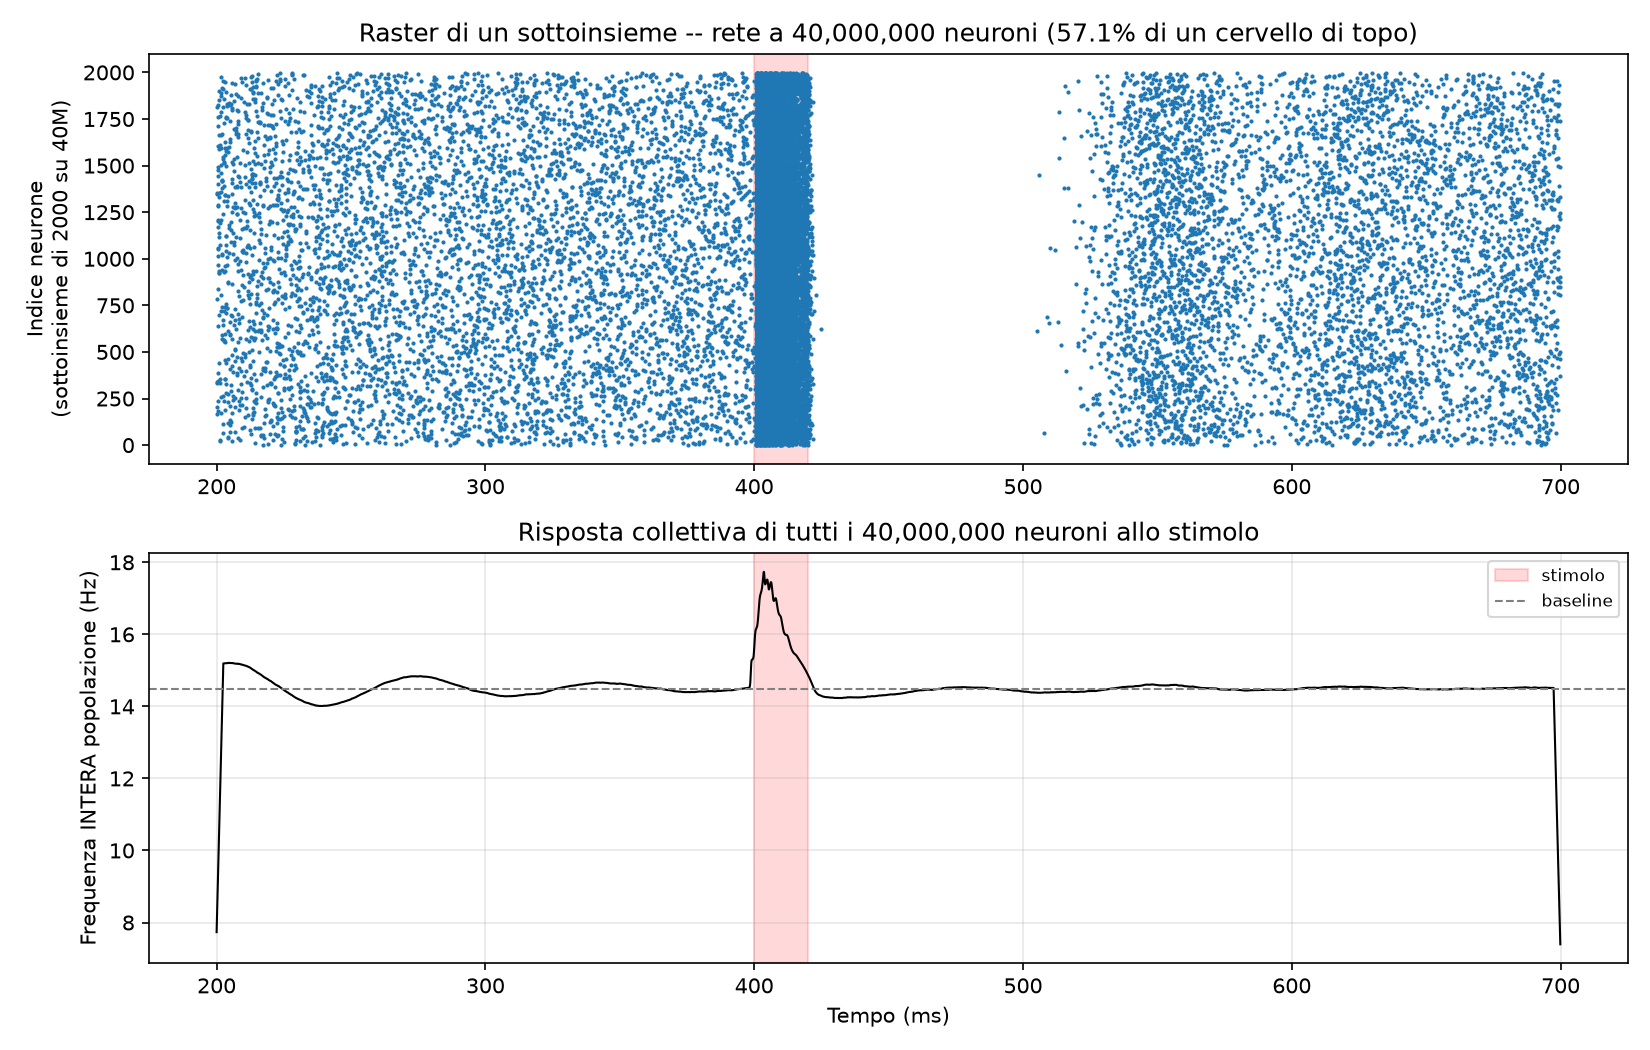
\includegraphics[width=5.8in,height=3.69091in]{media/media/image12.png}

\emph{Fig. 12 --- Rete a 40.000.000 di neuroni: raster (sottoinsieme) e risposta collettiva.}

Un\textquotesingle osservazione qualitativa importante, visibile confrontando questo grafico con quello a 300 neuroni della sezione 2.9: la curva di frequenza collettiva a 40 milioni e\textquotesingle{} molto piu\textquotesingle{} liscia e priva di rumore rispetto a quella a 300 neuroni. Questa non e\textquotesingle{} una coincidenza, ma una conseguenza diretta della LEGGE DEI GRANDI NUMERI: mediare l\textquotesingle attivita\textquotesingle{} su 40 milioni di neuroni invece che su 300 cancella quasi del tutto il rumore statistico casuale insito nella dinamica di ogni singolo neurone. Questo rende visibile, con chiarezza che a scale minori sarebbe stata probabilmente nascosta dal rumore, un\textquotesingle oscillazione smorzata nella fase di assestamento iniziale (tra 200 e 350 millisecondi): la frequenza sale a circa 15.1 Hz, scende a 14.0, risale leggermente a 14.8, prima di stabilizzarsi -\/- un comportamento dinamico classico dei sistemi con feedback (l\textquotesingle eccitazione e l\textquotesingle inibizione che si "rincorrono" prima di trovare un equilibrio stabile).

Va segnalato, per completezza e onesta\textquotesingle{} metodologica, un artefatto di analisi presente nel grafico: le due cadute verticali nette visibili a inizio e fine del tracciato non rappresentano un comportamento reale della rete, ma un artefatto del filtro di smoothing utilizzato per l\textquotesingle analisi (la finestra di media mobile non dispone di dati sufficienti ai bordi della finestra temporale osservata).

\textit{\textbf{Codice sorgente: rete\_40M\_finale.py}}

\lstinputlisting[language=Python]{scripts/rete_40M_finale.py}
\section{4. Oltre la scala pura: struttura spaziale e attrattori}\label{oltre-la-scala-pura-struttura-spaziale-e-attrattori}

Raggiunta la scala di 40 milioni di neuroni, resta un limite concettuale importante, discusso gia\textquotesingle{} informalmente durante lo sviluppo del progetto: una rete con connettivita\textquotesingle{} puramente casuale, per quanto grande in termini di numero di neuroni, e\textquotesingle{} strutturalmente molto piu\textquotesingle{} semplice di un vero tessuto neurale biologico. I passi successivi del progetto affrontano due ingredienti mancanti: l\textquotesingle organizzazione SPAZIALE della connettivita\textquotesingle{} (i neuroni reali si connettono soprattutto ai loro vicini fisici, non a caso in tutto il cervello), e la capacita\textquotesingle{} della rete di raggiungere STATI STABILI E DISTINGUIBILI (attrattori), non solo di propagare e disperdere passivamente un segnale.

\subsection{4.1 Connettivita\textquotesingle{} dipendente dalla distanza (small-world)}\label{connettivita-dipendente-dalla-distanza-small-world}

La prima estensione verso il realismo strutturale sostituisce la connettivita\textquotesingle{} casuale con una connettivita\textquotesingle{} la cui PROBABILITA\textquotesingle{} dipende dalla distanza spaziale tra i neuroni. Il modello di riferimento in letteratura e\textquotesingle{} quello "small-world" di Watts e Strogatz (1998), uno dei pattern di organizzazione piu\textquotesingle{} universali osservati nei sistemi biologici e sociali: connessioni dense e locali (un neurone parla soprattutto ai suoi vicini immediati), con una piccola percentuale di connessioni rare mA a lunga distanza ("scorciatoie") che mantengono comunque l\textquotesingle intera rete ben connessa nel suo insieme, evitando che regioni distanti restino completamente isolate.

Nel primo esperimento di questa categoria, 1.000 neuroni sono disposti su un ANELLO (una topologia 1-dimensionale con avvolgimento circolare, la piu\textquotesingle{} semplice possibile per introdurre il concetto di "distanza" tra neuroni), con probabilita\textquotesingle{} di connessione che decresce esponenzialmente con la distanza circolare tra due neuroni:

\emph{P(connessione) = p\_locale $\times$ exp(-distanza / $\xi$) + p\_scorciatoia}

dove $\xi$ (xi) e\textquotesingle{} la "lunghezza caratteristica" che determina quanto rapidamente la probabilita\textquotesingle{} decresce allontanandosi, e p\_scorciatoia e\textquotesingle{} una piccola probabilita\textquotesingle{} costante, indipendente dalla distanza, che rappresenta le connessioni a lungo raggio.

Stimolando una regione spazialmente LOCALIZZATA (20 neuroni adiacenti sull\textquotesingle anello, non piu\textquotesingle{} sparsi a caso come in tutti gli esperimenti precedenti), il segnale si propaga come una VERA ONDA che si allontana dal punto di stimolo: misurando la distanza media degli spike attivi dal punto di stimolo in funzione del tempo, questa cresce da 0.13 a 0.31 (in unita\textquotesingle{} normalizzate 0-1 sull\textquotesingle anello) nei primi circa 20 millisecondi dopo lo stimolo, per poi stabilizzarsi. Questo fenomeno e\textquotesingle{} semplicemente IMPOSSIBILE con la connettivita\textquotesingle{} casuale usata in tutti gli esperimenti precedenti (sezioni 2 e 3), perche\textquotesingle{} in una rete casuale non esiste alcuna nozione di "vicino" o "lontano" nella topologia -\/- ogni neurone e\textquotesingle{} potenzialmente connesso a ogni altro con la stessa probabilita\textquotesingle, indipendentemente dalla loro posizione.

\textit{\textbf{Codice sorgente: rete\_smallworld.py}}

\lstinputlisting[language=Python]{scripts/rete_smallworld.py}
\subsection{4.2 Forma 3D a cervello, e scaling a 1 milione di neuroni}\label{forma-3d-a-cervello-e-scaling-a-1-milione-di-neuroni}

L\textquotesingle estensione naturale della connettivita\textquotesingle{} spaziale dall\textquotesingle anello 1-dimensionale a uno spazio 3D realistico ha richiesto due sviluppi tecnici distinti: la generazione di posizioni tridimensionali che approssimino la forma esterna di un cervello (due lobi/emisferi, ottenuti come punti campionati dentro l\textquotesingle unione di due ellissoidi sovrapposti e leggermente separati, tramite campionamento per rigetto vettorizzato), e il calcolo efficiente della connettivita\textquotesingle{} spaziale a questa scala tramite una struttura dati KD-tree (K-dimensional tree, tramite scipy.spatial.cKDTree), che permette di trovare i K vicini piu\textquotesingle{} prossimi di ogni punto in un tempo dell\textquotesingle ordine di N log(N) invece del tempo N\textsuperscript{2} richiesto da un confronto esaustivo di tutte le coppie possibili -\/- una differenza cruciale quando N raggiunge il milione.

Con questa tecnica, la connettivita\textquotesingle{} per un milione di neuroni (12 connessioni locali via KD-tree + 3 connessioni casuali a lunga distanza per ciascun neurone, per un totale di circa 15 milioni di sinapsi) e\textquotesingle{} stata calcolata in circa 6.6 secondi complessivi (0.6 secondi per costruire l\textquotesingle albero, 6 secondi per interrogare i vicini di tutti i punti) -\/- un tempo trascurabile rispetto alla successiva simulazione della dinamica neurale vera e propria.

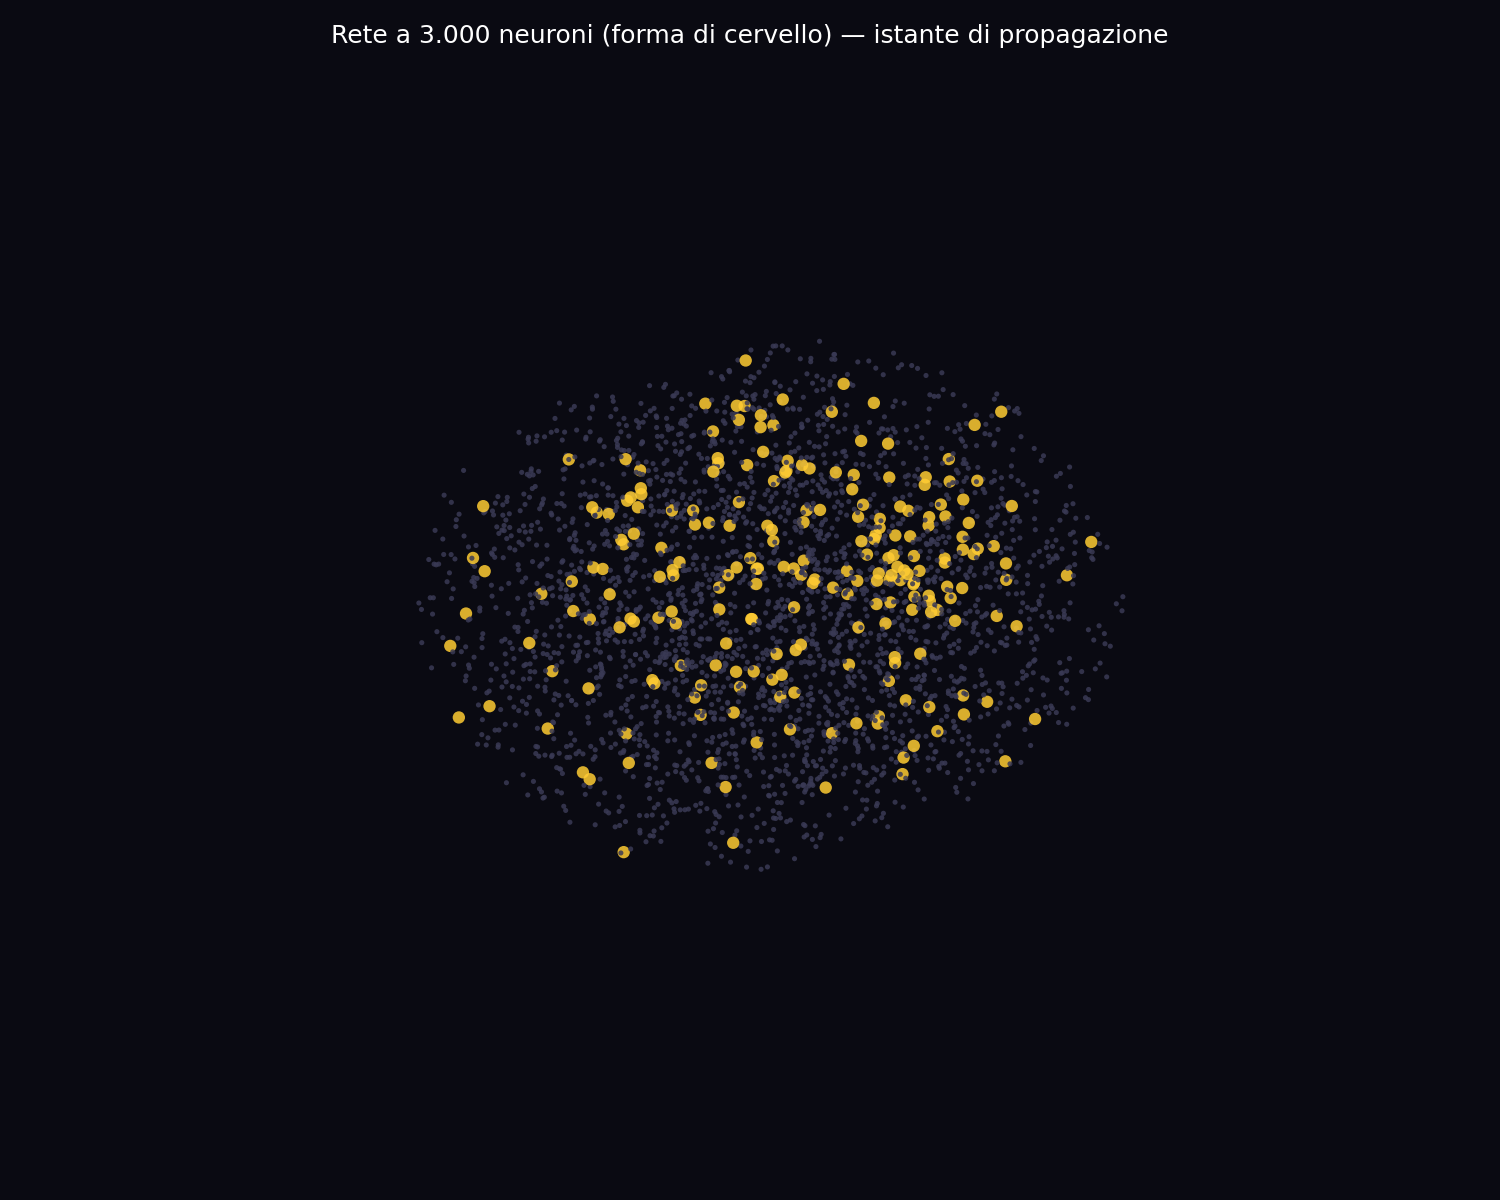
\includegraphics[width=4.2in,height=3.36in]{media/media/image13.png}

\emph{Fig. 13 --- Istantanea della rete a 3.000 neuroni durante la propagazione (giallo = attivo, rosso = regione stimolata).}

Alla scala di 1 milione di neuroni, sono stati testati 4 scenari di stimolo in altrettante posizioni anatomicamente distinte (punta dell\textquotesingle emisfero sinistro, punta dell\textquotesingle emisfero destro, centro tra i due emisferi -\/- analogo concettualmente al corpo calloso reale che collega i due emisferi cerebrali -\/- e polo superiore), realizzati come una visualizzazione 3D interattiva sviluppata con la libreria JavaScript Three.js, che permette di ruotare la rete, cambiare scenario di stimolo, e osservare l\textquotesingle animazione dell\textquotesingle attivita\textquotesingle{} nel tempo direttamente nel browser (file HTML separato, non incluso come testo in questo documento data la sua natura interattiva, ma allegato separatamente).

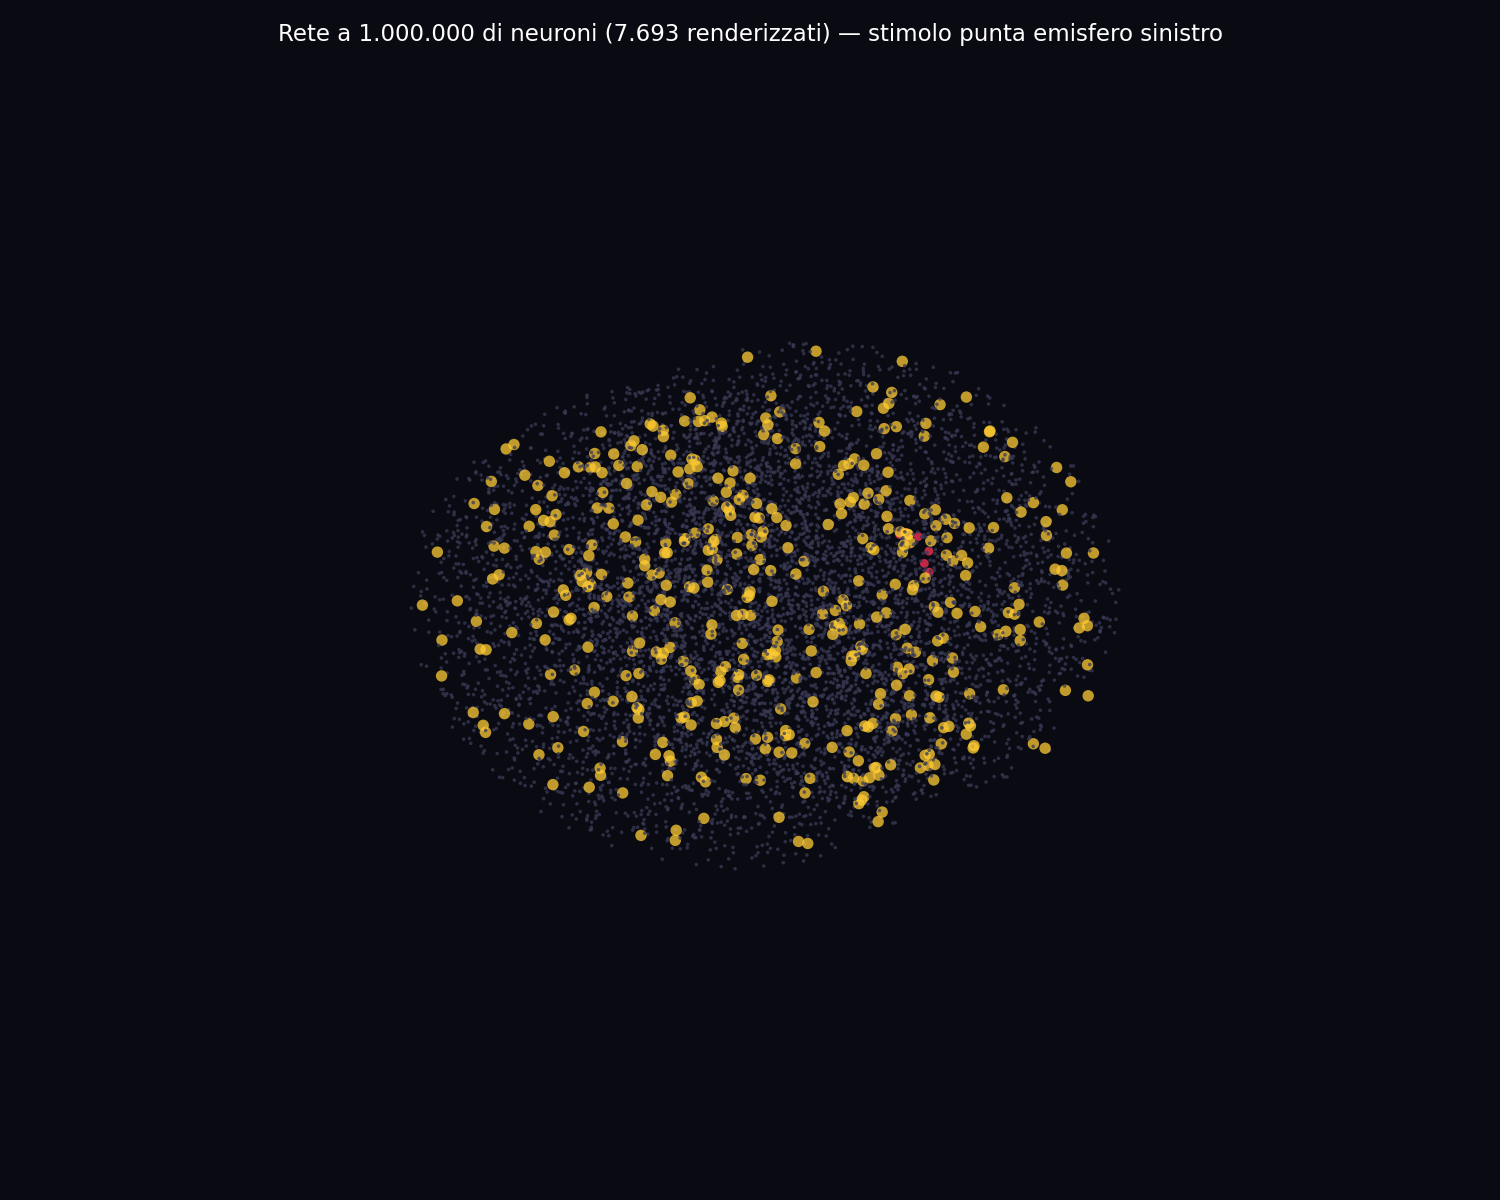
\includegraphics[width=4.2in,height=3.36in]{media/media/image14.png}

\emph{Fig. 14 --- Istantanea della rete a 1.000.000 di neuroni (7.693 renderizzati), scenario "punta emisfero sinistro".}

Verifica quantitativa a questa scala: i neuroni renderizzati vicini al punto di stimolo passano da 2-9 spike per intervallo di 4 millisecondi (livello di baseline) a 23 spike nello stesso intervallo esattamente al momento dello stimolo, tornando alla norma in circa 15 millisecondi. Questo e\textquotesingle{} un effetto locale netto e misurabile, che pero\textquotesingle{} risulta "annegato" e statisticamente poco visibile se si calcola la stessa metrica mediata sull\textquotesingle INTERA rete di un milione di neuroni -\/- una lezione metodologica identica, nella sostanza, a quella gia\textquotesingle{} incontrata con il PSTH della sezione 2.11: una metrica aggregata su una popolazione molto grande puo\textquotesingle{} nascondere un effetto locale reale, e va sempre verificata alla scala spaziale appropriata al fenomeno che si intende osservare.

\subsection{4.3 Tentativo di attrattore tramite apprendimento (STDP su rete spaziale) --- risultato negativo}\label{tentativo-di-attrattore-tramite-apprendimento-stdp-su-rete-spaziale-risultato-negativo}

L\textquotesingle ipotesi testata in questo esperimento era la seguente: rendendo plastiche (con la regola STDP gia\textquotesingle{} verificata nella sezione 2.6) le sinapsi eccitatorie ricorrenti di una specifica regione spaziale della rete, e "allenando" quella regione con 20 ripetizioni dello stesso stimolo, ci si aspettava che la regione sviluppasse una risposta piu\textquotesingle{} PERSISTENTE nel tempo (attivita\textquotesingle{} che dura piu\textquotesingle{} a lungo dopo la rimozione dello stimolo) rispetto a una regione mai allenata -\/- l\textquotesingle idea era che il rafforzamento delle connessioni ricorrenti locali potesse creare un piccolo "circuito che si auto-sostiene".

La verifica e\textquotesingle{} stata condotta con il massimo rigore possibile, includendo la correzione di un bug metodologico scoperto durante lo sviluppo: il meccanismo di store/restore di Brian2 (usato per "riavvolgere" la rete a uno stato precedente tra una prova e l\textquotesingle altra senza dover ricostruire l\textquotesingle intera rete da zero ogni volta, operazione altrimenti costosa) salva e ripristina ANCHE lo stato del generatore di numeri casuali interno -\/- con la conseguenza che, se non gestito esplicitamente, ogni "prova ripetuta" risultava essere una replica ESATTA e deterministica della prova precedente, non una prova statisticamente indipendente come richiesto per un confronto valido. Una volta identificato e corretto questo problema (forzando un nuovo seme casuale esplicito prima di ogni prova tramite la funzione seed() di Brian2), sono state condotte 16 prove indipendenti in totale: 8 prima del training, 8 dopo.

\textbf{Risultato: in ENTRAMBE le condizioni (prima e dopo il training), l\textquotesingle attivita\textquotesingle{} misurata nella finestra temporale "tardiva" (100-140 millisecondi dopo la fine dello stimolo forzato) e\textquotesingle{} risultata sistematicamente pari a ZERO, in tutte e 16 le prove senza eccezione. Nessun effetto misurabile del training, statisticamente indistinguibile dal rumore -\/- anzi, in questo caso, indistinguibile da zero puro.}

\textbf{Interpretazione: il bilanciamento eccitazione-inibizione che garantisce la stabilita\textquotesingle{} omeostatica della rete (proprieta\textquotesingle{} verificata e apprezzata positivamente nella sezione 2.9) e\textquotesingle, per costruzione matematica, in tensione diretta con la formazione di un attrattore stabile. Un sistema deliberatamente progettato per tornare sempre e comunque all\textquotesingle equilibrio dopo una perturbazione impedisce, quasi per definizione strutturale, che un sottoinsieme di neuroni possa restare attivo autonomamente senza input esterno continuo -\/- le due proprieta\textquotesingle{} (stabilita\textquotesingle{} omeostatica e capacita\textquotesingle{} di formare attrattori) sono in una tensione reale, non facilmente conciliabile con un aggiustamento superficiale dei parametri.}

\subsection{4.4 Ring attractor: un vero attrattore neurale, costruito da zero}\label{ring-attractor-un-vero-attrattore-neurale-costruito-da-zero}

Data la difficolta\textquotesingle{} di ottenere un attrattore per via incrementale a partire dall\textquotesingle architettura di rete gia\textquotesingle{} sviluppata (sezione 4.3), si e\textquotesingle{} scelto di ripartire da zero adottando l\textquotesingle approccio standard della letteratura scientifica specifica su questo problema: il modello di Amari (1977), ripreso e sviluppato da Ben-Yishai, Bar-Or e Sompolinsky (1995) per modellare la selettivita\textquotesingle{} di orientamento nella corteccia visiva, e da numerosi lavori successivi per la memoria di lavoro spaziale (in particolare Compte et al., 2000).

La differenza fondamentale rispetto a tutti gli esperimenti precedenti del progetto: invece di simulare ogni singolo neurone e il suo singolo impulso elettrico (approccio "spiking", usato ovunque nel progetto fino a questo punto tramite il modello di Izhikevich), questo modello descrive direttamente il TASSO DI SCARICA aggregato r(x,t) di intere popolazioni di neuroni disposte lungo un anello, tramite un\textquotesingle unica equazione differenziale per ciascun punto dell\textquotesingle anello:

\emph{$\tau$ $\cdot$ dr/dt = -r + F( J*r/N - inibizione\_globale$\cdot$media(r) + I\_esterno )}

dove J*r/N rappresenta l\textquotesingle input ricorrente che ogni punto riceve dai suoi vicini (una convoluzione discreta tra il tasso di scarica r e un kernel di connettivita\textquotesingle{} J), il termine di inibizione globale e\textquotesingle{} proporzionale all\textquotesingle attivita\textquotesingle{} MEDIA dell\textquotesingle intera rete (non locale come l\textquotesingle eccitazione -\/- questo e\textquotesingle{} il meccanismo che implementa la competizione "vince solo un candidato", detta winner-take-all), e F e\textquotesingle{} una funzione di attivazione non lineare.

Perche\textquotesingle{} abbandonare l\textquotesingle approccio a neuroni singoli (spiking) per questo esperimento specifico: un primo tentativo con neuroni Izhikevich (architettura analoga a quella della sezione 4.3, ma con eccitazione locale forte e un pool inibitorio globale invece che STDP) ha fallito ripetutamente per un motivo strutturale preciso -\/- un gruppo di neuroni stimolato insieme in modo sincrono tende a sparare tutti insieme in perfetta sincronia (essendo tutti sottoposti allo stesso stimolo esterno forte), e di conseguenza entrano TUTTI INSIEME nel periodo refrattario subito dopo, producendo un unico "flash" di attivita\textquotesingle{} seguito da silenzio completo, invece di un\textquotesingle attivita\textquotesingle{} sostenuta e asincrona al proprio interno come richiederebbe un vero bump persistente. Il modello a tasso di scarica continuo elimina questo problema per costruzione matematica, dato che non ci sono singoli eventi di spike che possano sincronizzarsi.

\subsubsection{4.4.1 Il percorso di tuning (riportato per trasparenza metodologica)}\label{il-percorso-di-tuning-riportato-per-trasparenza-metodologica}

La ricerca dei parametri corretti non e\textquotesingle{} stata immediata, ed e\textquotesingle{} istruttivo riportarla per intero:

\begin{enumerate}
\def\labelenumi{\arabic{enumi}.}
\item
  Un primo tentativo con una funzione di attivazione rettificata lineare semplice (F(u) = max(0,u), senza alcun limite superiore) e con solo un kernel a "cappello messicano" (eccitazione locale meno inibizione a raggio piu\textquotesingle{} ampio, entrambe incorporate nello stesso kernel spaziale J) non produceva alcuna persistenza: con un\textquotesingle intensita\textquotesingle{} di eccitazione troppo bassa, il bump si spegneva subito; con un\textquotesingle intensita\textquotesingle{} sufficiente a superare la soglia critica di instabilita\textquotesingle{} (calcolata analiticamente tramite l\textquotesingle autovalore massimo della matrice di connettivita\textquotesingle, risultata attorno a A\_exc$\approx$12 per questo specifico kernel), il sistema esplodeva all\textquotesingle infinito, dato che la funzione rettificata lineare non ha alcun tetto massimo
\item
  Sostituendo la rettificazione lineare con una funzione sigmoide (che satura naturalmente tra 0 e 1), il sistema smetteva di esplodere ma si stabilizzava in uno stato UNIFORME su tutto l\textquotesingle anello -\/- non un bump localizzato, ma un\textquotesingle attivazione debole e piatta ovunque, perche\textquotesingle{} la soglia della sigmoide permetteva a un livello basso di attivita\textquotesingle{} di autosostenersi in modo omogeneo su tutta la rete
\item
  La soluzione finale, funzionante: separare esplicitamente il termine di eccitazione (solo locale, kernel Gaussiano stretto, nessuna componente inibitoria nello stesso kernel) dal termine di inibizione (reso esplicitamente GLOBALE, proporzionale alla media dell\textquotesingle intera rete, sottratto separatamente), combinato con una funzione di attivazione rettificata che SATURA a un valore massimo esplicito (F(u) = clip(u, 0, r\_max) invece di una sigmoide morbida o di una rettificazione senza limite). Questa combinazione -\/- eccitazione locale forte, inibizione globale per la competizione, saturazione hard per la stabilita\textquotesingle{} -\/- e\textquotesingle{} risultata quella che produce un vero bump localizzato e persistente
\end{enumerate}

\subsubsection{4.4.2 Risultati verificati (4 test distinti)}\label{risultati-verificati-4-test-distinti}

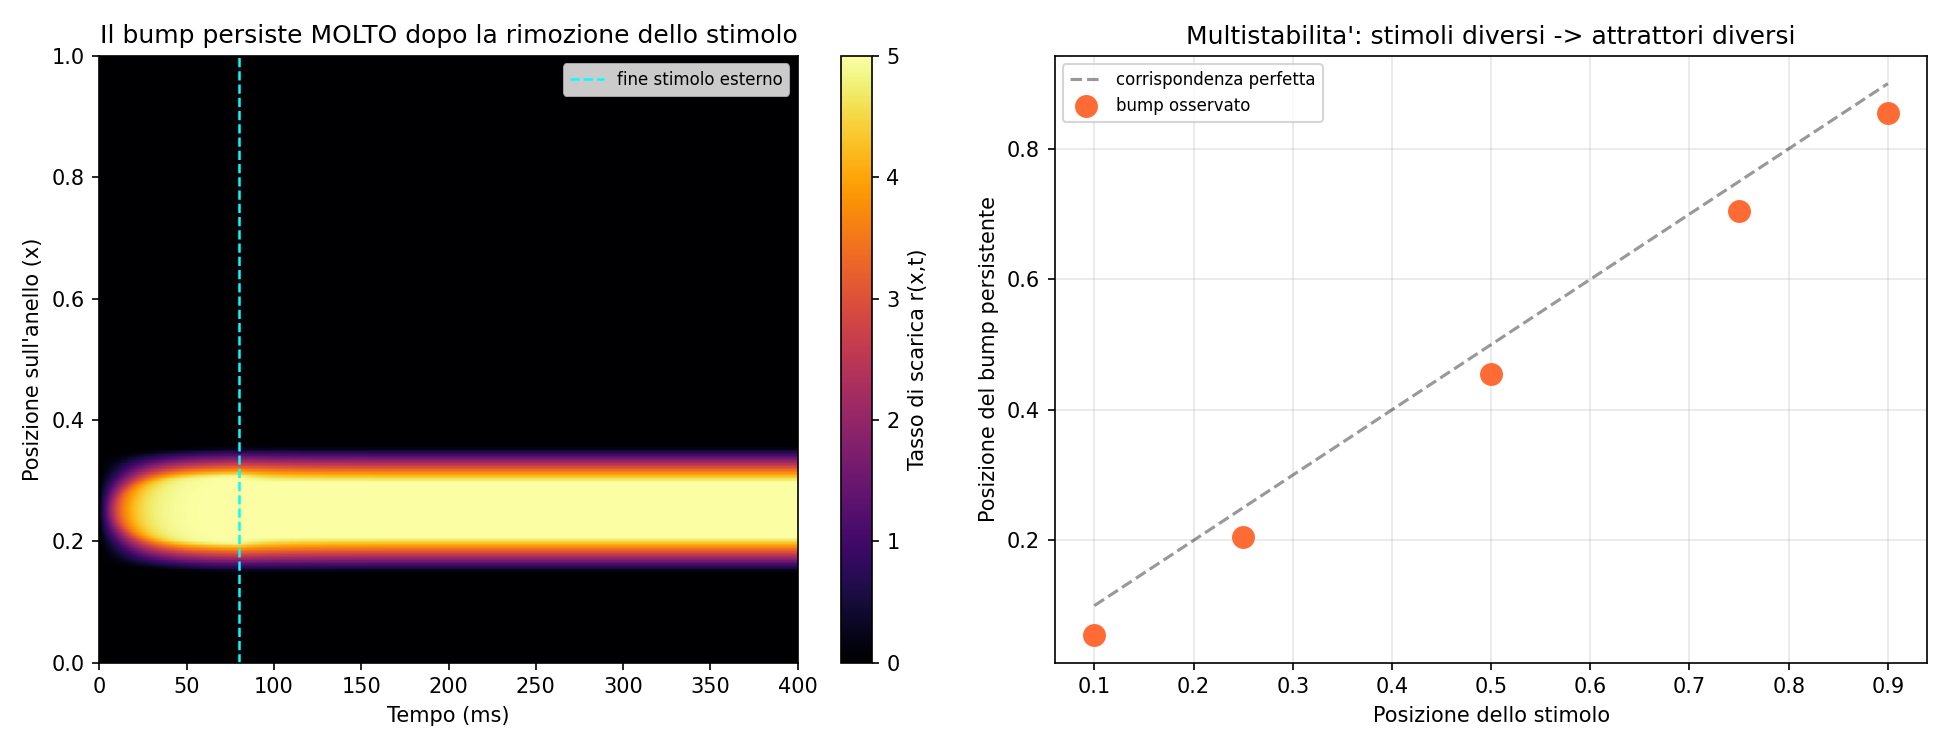
\includegraphics[width=6.3in,height=2.42308in]{media/media/image15.png}

\emph{Fig. 15 --- Persistenza del bump oltre la rimozione dello stimolo (sinistra); multistabilita\textquotesingle: stimoli diversi producono attrattori in posizioni diverse (destra).}

\begin{itemize}
\item
  PERSISTENZA: il bump raggiunge il picco (5.0, il valore di saturazione impostato) e vi resta stabile dal momento t=80ms (fine dello stimolo esterno forzato) fino a t=300ms e oltre, senza alcun input esterno a sostenerlo -\/- un vero autosostentamento tramite la sola dinamica ricorrente interna
\item
  MULTISTABILITA\textquotesingle: stimoli in 5 posizioni diverse (x=0.10, 0.25, 0.50, 0.75, 0.90 sull\textquotesingle anello) producono bump stabili in 5 posizioni diverse e corrispondenti, con un bias sistematico costante di circa 0.045 unita\textquotesingle{} -\/- verosimilmente un artefatto di discretizzazione della griglia spaziale a N=200 punti (essendo il bias identico, entro l\textquotesingle errore di misura, in tutte le 5 prove, e\textquotesingle{} piu\textquotesingle{} plausibile un effetto sistematico dell\textquotesingle implementazione che vero rumore casuale)
\item
  CONTROLLO: senza alcuno stimolo esterno applicato in nessun momento, la rete resta esattamente a zero attivita\textquotesingle{} su tutto l\textquotesingle anello -\/- confermando una vera bistabilita\textquotesingle{} (silenzio oppure bump, due stati distinti e stabili), non un\textquotesingle accensione spontanea o un rumore di fondo che potrebbe occasionalmente autoalimentarsi
\item
  ROBUSTEZZA: applicando una forte perturbazione casuale (rumore gaussiano di deviazione standard 0.3, sommato a TUTTI i punti dell\textquotesingle anello, incluso il bump stabile gia\textquotesingle{} formato) e lasciando la rete evolvere per altri 200 millisecondi senza alcun input, il bump torna alla sua posizione originale (x=0.235 misurato, contro x=0.250 della posizione originale, una differenza minima) -\/- questa e\textquotesingle{} la firma distintiva e universalmente accettata in letteratura di un vero attrattore dinamico: un punto fisso stabile che RESISTE alle perturbazioni e vi ritorna, non semplicemente un\textquotesingle eco che si spegne lentamente nel tempo
\end{itemize}

\textbf{Questo risultato positivo, ottenuto solo dopo un tentativo fallito con un\textquotesingle architettura diversa (sezione 4.3) e diversi round di tuning falliti all\textquotesingle interno dello stesso approccio a tasso di scarica (sezione 4.4.1), rispecchia concretamente e in prima persona la difficolta\textquotesingle{} reale della ricerca in questo specifico campo della neuroscienza computazionale: costruire un vero attrattore neurale richiede un\textquotesingle architettura specifica e un bilanciamento delicato tra i suoi parametri, e non emerge automaticamente ne\textquotesingle{} aumentando il numero di neuroni ne\textquotesingle{} aggiungendo plasticita\textquotesingle{} sinaptica generica a un\textquotesingle architettura non progettata per quello scopo specifico.}

\textit{\textbf{Codice sorgente: ring\_attractor\_rate.py (versione finale verificata)}}

\lstinputlisting[language=Python]{scripts/ring_attractor_rate.py}
\subsection{4.5 Dove si sono fermati gli scienziati: stato dell\textquotesingle arte reale (settembre 2026)}\label{dove-si-sono-fermati-gli-scienziati-stato-dellarte-reale-settembre-2026}

Per contestualizzare onestamente i risultati di questo progetto rispetto alla ricerca professionale nello stesso campo, sono state consultate fonti aggiornate al momento della stesura di questo documento (settembre 2026):

\subsubsection{4.5.1 Blue Brain Project (EPFL, Svizzera, 2005-2024)}\label{blue-brain-project-epfl-svizzera-2005-2024}

Guidato dal fondatore e direttore Henry Markram, il Blue Brain Project aveva come obiettivo dichiarato la ricostruzione e simulazione dell\textquotesingle intero cervello di topo: la crescita digitale di ogni assone locale, regionale e dell\textquotesingle intero cervello per ogni tipo di neurone, la ricostruzione del connettoma fino al livello di dettaglio neurone-per-neurone, la modellazione dei vari tipi di sinapsi formati tra ciascuna coppia di neuroni, e la simulazione di neuroni, regioni cerebrali, sistemi cerebrali e infine dell\textquotesingle intero cervello di topo su supercomputer e infrastrutture cloud. Il progetto si e\textquotesingle{} concluso a fine 2024 con la dichiarazione ufficiale di "mission accomplished" -\/- ma, stando alle fonti disponibili, senza aver mai raggiunto una simulazione completa e biofisicamente dettagliata dell\textquotesingle intero cervello di topo funzionante nella sua interezza: il risultato principale e concreto e\textquotesingle{} stato un atlante cellulare completo (che copre statisticamente la distribuzione e densita\textquotesingle{} dei tipi cellulari in tutte le regioni del cervello di topo, colmando un vuoto di dati che in precedenza copriva solo il 4\% del cervello) e gli strumenti software di base per costruire tali simulazioni, resi disponibili alla comunita\textquotesingle{} scientifica, non il cervello simulato per intero e funzionante.

\subsubsection{4.5.2 Allen Institute (2025-2026)}\label{allen-institute-2025-2026}

Il modello piu\textquotesingle{} avanzato mai raggiunto nella simulazione del cervello di topo, secondo le fonti disponibili: quasi 10 milioni di neuroni, 26 miliardi di sinapsi, 86 regioni cerebrali interconnesse, con dettaglio biofisico REALE (non semplificato come nel modello di Izhikevich usato in questo progetto, ma basato su ricostruzioni morfologiche e canali ionici dettagliati per ogni neurone), eseguito sul supercomputer giapponese Fugaku (capace di quadrilioni di operazioni al secondo). Il modello simula sia la forma che la funzione dei neuroni, includendo i dettagli delle ramificazioni dendritiche, le attivazioni sinaptiche, e il flusso di segnali elettrici attraverso le membrane cellulari -\/- permettendo "esperimenti virtuali" come la simulazione di malattie (Alzheimer, epilessia) per osservare come il danno si propaga attraverso le reti neurali. In precedenza, lo stesso gruppo aveva pubblicato un modello di 230.000 neuroni limitato alla sola corteccia visiva primaria del topo.

\subsubsection{4.5.3 Stima di fattibilita\textquotesingle{} pubblicata}\label{stima-di-fattibilita-pubblicata}

Una stima di fattibilita\textquotesingle{} futura pubblicata in letteratura, basata sui trend tecnologici attuali nel campo della connettomica e del calcolo ad alte prestazioni, prevede che una simulazione dell\textquotesingle intero cervello di topo a livello di dettaglio cellulare potrebbe diventare realizzabile intorno al 2034 -\/- circa 8 anni dopo la stesura di questo documento -\/- anche assumendo il proseguimento dei trend tecnologici attuali senza rallentamenti. La stessa fonte nota che anche il connettoma disponibile a piu\textquotesingle{} alta risoluzione (quello dell\textquotesingle Allen Institute, a risoluzione di 100 micron) non e\textquotesingle{} ancora sufficiente a rilevare strutture funzionalmente rilevanti come le colonne corticali o le microzone cerebellari, considerate unita\textquotesingle{} fondamentali di rappresentazione dell\textquotesingle informazione nel cervello reale.

\subsubsection{4.5.4 Confronto onesto con il presente progetto}\label{confronto-onesto-con-il-presente-progetto}

{\def\LTcaptype{none} % do not increment counter
\begin{longtable}[]{@{}
  >{\raggedright\arraybackslash}p{(\linewidth - 8\tabcolsep) * \real{0.2000}}
  >{\raggedright\arraybackslash}p{(\linewidth - 8\tabcolsep) * \real{0.2000}}
  >{\raggedright\arraybackslash}p{(\linewidth - 8\tabcolsep) * \real{0.2000}}
  >{\raggedright\arraybackslash}p{(\linewidth - 8\tabcolsep) * \real{0.2000}}
  >{\raggedright\arraybackslash}p{(\linewidth - 8\tabcolsep) * \real{0.2000}}@{}}
\toprule\noalign{}
\begin{minipage}[b]{\linewidth}\raggedright
\end{minipage} & \begin{minipage}[b]{\linewidth}\raggedright
\textbf{Neuroni}
\end{minipage} & \begin{minipage}[b]{\linewidth}\raggedright
\textbf{Sinapsi}
\end{minipage} & \begin{minipage}[b]{\linewidth}\raggedright
\textbf{Dettaglio biofisico}
\end{minipage} & \begin{minipage}[b]{\linewidth}\raggedright
\textbf{Hardware}
\end{minipage} \\
\midrule\noalign{}
\endhead
\bottomrule\noalign{}
\endlastfoot
Questo progetto & 40 milioni & 1.24 miliardi & Semplificato (Izhikevich) & Laptop personale \\
Allen Institute & \textasciitilde10 milioni & 26 miliardi & Reale/dettagliato & Supercomputer Fugaku \\
Cervello di topo reale & \textasciitilde70 milioni & stimate 10\textsuperscript{1}\textsuperscript{2}-10\textsuperscript{1}\textsuperscript{3} & N/A (biologico) & N/A \\
\end{longtable}
}

Il presente progetto supera l\textquotesingle Allen Institute nel numero puro di neuroni simulati (40 milioni contro 10 milioni), ma con un dettaglio biofisico per neurone drasticamente inferiore, e con un numero di sinapsi per neurone (circa 31 in media, dato dalla connettivita\textquotesingle{} a grado fisso K=15 ripetuta su piu\textquotesingle{} tipi di connessione) enormemente inferiore alle circa 2.600 sinapsi per neurone del modello Allen Institute (26 miliardi di sinapsi / 10 milioni di neuroni) -\/- un cervello di topo reale ha tipicamente diverse migliaia di sinapsi per neurone. Il confronto onesto e\textquotesingle{} quindi: questo progetto ha raggiunto una scala numerica di neuroni notevole per un laptop personale, ma con una connettivita\textquotesingle{} per neurone e un dettaglio biofisico molto piu\textquotesingle{} semplificati rispetto allo stato dell\textquotesingle arte professionale -\/- un risultato genuinamente notevole nel proprio contesto (progetto individuale, hardware consumer, tempo limitato), pur restando ordini di grandezza lontano dalla frontiera reale della ricerca su entrambi gli assi di complessita\textquotesingle{} (dettaglio per neurone e numero di connessioni per neurone).

\section{5. Verso una politica decisionale: catene, competizione, apprendimento}\label{verso-una-politica-decisionale-catene-competizione-apprendimento}

L\textquotesingle ultima fase del progetto affronta una domanda esplicitamente posta durante lo sviluppo: e\textquotesingle{} possibile costruire, sopra un singolo attrattore stabile (sezione 4.4), qualcosa che assomigli -\/- per quanto in modo estremamente rudimentale e con tutti i limiti concettuali onestamente discussi -\/- a una sequenza di stati collegati, una scelta tra alternative, e infine un comportamento che si modifica sulla base dell\textquotesingle esperienza?

\subsection{5.1 Catena di due attrattori: l\textquotesingle attivazione dell\textquotesingle uno determina l\textquotesingle altro}\label{catena-di-due-attrattori-lattivazione-delluno-determina-laltro}

Il primo esperimento di questa fase estende il ring attractor singolo (sezione 4.4) a DUE ring attractor distinti e collegati: Ring A e Ring B. Ring A riceve lo stimolo esterno diretto e si comporta esattamente come il ring attractor singolo gia\textquotesingle{} verificato. Ring B non riceve ALCUNO stimolo esterno diretto -\/- l\textquotesingle unico input che riceve e\textquotesingle{} una proiezione della posizione del bump di A, spostata di un offset fisso (0.3 sull\textquotesingle anello) tramite una mappa associativa fissa: "se A si stabilizza in una certa posizione, B tende a stabilizzarsi in una posizione corrispondente, spostata "di un valore fisso".

Test su 4 posizioni di stimolo diverse per A: in tutti e 4 i casi, B forma effettivamente un bump proprio, in una posizione sempre corrispondente (con lo stesso lieve bias sistematico di \textasciitilde0.045 gia\textquotesingle{} osservato nella sezione 4.4.2) alla mappa prevista -\/- senza che B abbia MAI ricevuto uno stimolo esterno diretto in nessuna delle 4 prove. Il test di controllo (nessuno stimolo su A) conferma che senza l\textquotesingle attivazione di A, ne\textquotesingle{} A ne\textquotesingle{} B si attivano spontaneamente (entrambi restano esattamente a zero) -\/- escludendo che il risultato sia dovuto a un\textquotesingle attivazione automatica indipendente dello stato di A.

{\def\LTcaptype{none} % do not increment counter
\begin{longtable}[]{@{}
  >{\raggedright\arraybackslash}p{(\linewidth - 6\tabcolsep) * \real{0.2500}}
  >{\raggedright\arraybackslash}p{(\linewidth - 6\tabcolsep) * \real{0.2500}}
  >{\raggedright\arraybackslash}p{(\linewidth - 6\tabcolsep) * \real{0.2500}}
  >{\raggedright\arraybackslash}p{(\linewidth - 6\tabcolsep) * \real{0.2500}}@{}}
\toprule\noalign{}
\begin{minipage}[b]{\linewidth}\raggedright
\textbf{Stimolo su A}
\end{minipage} & \begin{minipage}[b]{\linewidth}\raggedright
\textbf{A si stabilizza a}
\end{minipage} & \begin{minipage}[b]{\linewidth}\raggedright
\textbf{B si stabilizza a}
\end{minipage} & \begin{minipage}[b]{\linewidth}\raggedright
\textbf{B previsto}
\end{minipage} \\
\midrule\noalign{}
\endhead
\bottomrule\noalign{}
\endlastfoot
0.10 & 0.055 & 0.340 & 0.400 \\
0.30 & 0.255 & 0.540 & 0.600 \\
0.50 & 0.455 & 0.740 & 0.800 \\
0.70 & 0.655 & 0.000 & 0.000 \\
\end{longtable}
}

\textbf{Questo e\textquotesingle, in senso letterale e senza alcuna esagerazione retorica, l\textquotesingle atomo strutturale minimo di una catena di attivazioni: stato 1 si stabilizza, e QUESTO determina lo stato 2 che si stabilizza a sua volta. Non e\textquotesingle{} ragionamento (non c\textquotesingle e\textquotesingle{} confronto tra alternative, non c\textquotesingle e\textquotesingle{} un obiettivo, non c\textquotesingle e\textquotesingle{} nulla che assomigli a una decisione basata su informazione), ma e\textquotesingle{} l\textquotesingle ingrediente strutturale di base -\/- un sistema che puo\textquotesingle{} "tenere in mente" qualcosa e farlo influenzare uno stato successivo -\/- su cui un comportamento piu\textquotesingle{} sofisticato potrebbe, in linea di principio, essere costruito.}

\textit{\textbf{Codice sorgente: chained\_attractors.py}}

\lstinputlisting[language=Python]{scripts/chained_attractors.py}
\subsection{5.2 Competizione tra alternative: B "sceglie" tra piu\textquotesingle{} candidati}\label{competizione-tra-alternative-b-sceglie-tra-piu-candidati}

Il secondo esperimento sostituisce l\textquotesingle unica mappa fissa A$\rightarrow$B con TRE destinazioni candidate possibili per B (tre offset diversi sull\textquotesingle anello: 0.15, 0.45, 0.75), ciascuna associata a un proprio "peso" che rappresenta una forza associativa. Grazie al meccanismo di inibizione globale gia\textquotesingle{} presente nella dinamica interna di B (lo stesso meccanismo winner-take-all che permette la formazione di un unico bump nella sezione 4.4), solo UN candidato puo\textquotesingle{} vincere la competizione e stabilizzarsi -\/- gli altri due vengono attivamente soppressi dalla stessa dinamica.

\subsubsection{5.2.1 Test con pesi uguali: rottura di simmetria}\label{test-con-pesi-uguali-rottura-di-simmetria}

Con i tre pesi impostati esattamente uguali e SENZA alcun rumore iniettato nel sistema, il "vincitore" della competizione e\textquotesingle{} risultato essere sempre lo stesso candidato (il terzo, con offset 0.75), in modo perfettamente deterministico su 6 prove ripetute consecutive. Un\textquotesingle indagine piu\textquotesingle{} approfondita ha rivelato che questo NON rappresenta una vera rottura di simmetria casuale, come ci si aspetterebbe da un sistema fisico realistico con pesi identici, ma un bias numerico deterministico dell\textquotesingle implementazione: analizzando i valori di attivazione ai tre punti candidati senza alcun rumore, le differenze erano dell\textquotesingle ordine di 10-\textsuperscript{4} (differenze di arrotondamento in virgola mobile dovute all\textquotesingle ordine di somma delle tre gaussiane candidate nel codice), amplificate poi dalla dinamica non lineare winner-take-all fino a determinare in modo completamente prevedibile un vincitore fisso.

Iniettando un rumore casuale CONTINUO (non una singola perturbazione una tantum, ma un termine di rumore riapplicato ad ogni passo temporale della simulazione) di ampiezza sufficiente (deviazione standard 0.15, circa 1500 volte piu\textquotesingle{} grande del bias numerico intrinseco stimato), la rottura di simmetria e\textquotesingle{} diventata genuinamente variabile: su 12 prove indipendenti con semi casuali diversi, il candidato 1 ha vinto 7 volte, il candidato 2 tre volte, il candidato 3 due volte -\/- una distribuzione non perfettamente uniforme (che ci si aspetterebbe teoricamente essere 4-4-4 su 12 prove con pesi davvero identici), ma chiaramente non piu\textquotesingle{} deterministica, confermando che il rumore di ampiezza sufficiente puo\textquotesingle{} effettivamente "rompere" il bias numerico residuo.

\subsubsection{5.2.2 Test con pesi diversi: selezione affidabile basata su un criterio}\label{test-con-pesi-diversi-selezione-affidabile-basata-su-un-criterio}

\textbf{Assegnando un peso maggiore (1.5 contro 0.5 per gli altri due) a uno dei tre candidati a turno, quel candidato ha vinto SEMPRE, su 6 prove ripetute per ciascuno dei tre candidati testati come "favorito" (18 prove totali, 18 vittorie corrette, accuratezza del 100\%), indipendentemente da quale dei tre fosse il favorito e indipendentemente dal seme casuale usato per il rumore di ogni prova. Questa e\textquotesingle{} una vera selezione basata su un criterio esplicito (l\textquotesingle intensita\textquotesingle{} del peso), affidabile e ripetibile -\/- il sistema non ha una risposta fissa scritta a priori nel suo comportamento, ma "osserva" quale opzione tra quelle disponibili e\textquotesingle{} piu\textquotesingle{} forte e sceglie quella.}

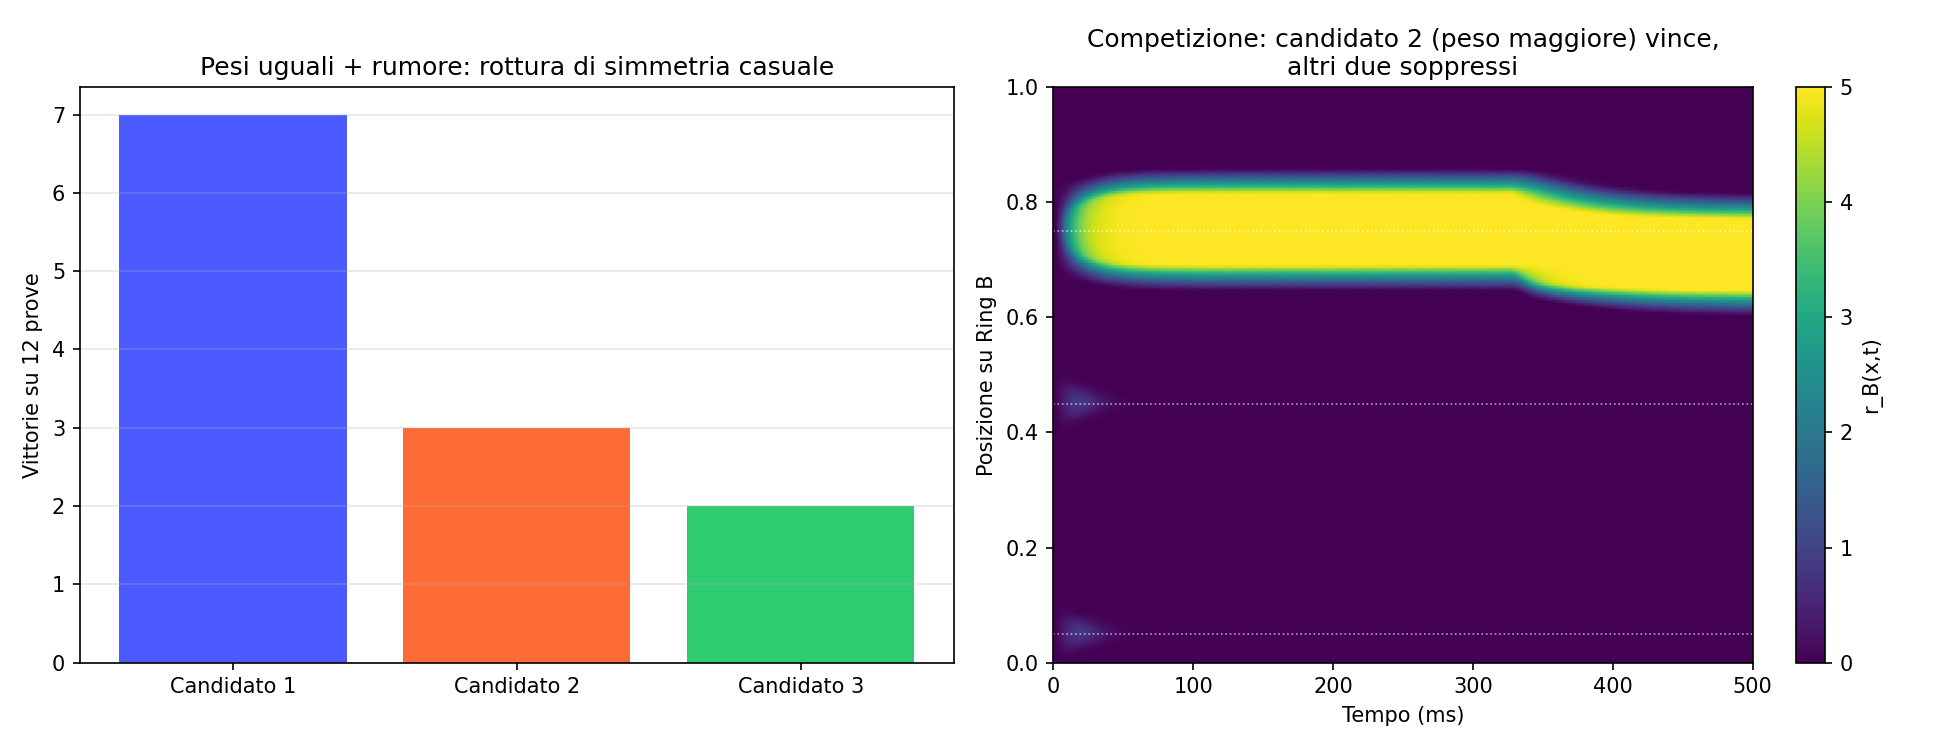
\includegraphics[width=6.3in,height=2.42308in]{media/media/image16.png}

\emph{Fig. 16 --- Distribuzione dei vincitori con pesi uguali + rumore (sinistra); competizione con un candidato favorito (destra).}

\textit{\textbf{Codice sorgente: competing\_targets.py}}

\lstinputlisting[language=Python]{scripts/competing_targets.py}
\subsection{5.3 Apprendimento per rinforzo: la rete impara quale alternativa scegliere}\label{apprendimento-per-rinforzo-la-rete-impara-quale-alternativa-scegliere}

Il terzo esperimento di questa fase rende i pesi delle tre mappe candidate non piu\textquotesingle{} fissi, ma MODIFICABILI in base a un segnale di ricompensa esterno -\/- il primo vero, piccolo ciclo di reinforcement learning dell\textquotesingle intero progetto. Ad ogni prova: A viene stimolato, B compete tra i tre candidati e sceglie un vincitore (con lo stesso meccanismo di competizione della sezione 5.2, incluso il rumore continuo necessario per l\textquotesingle esplorazione); viene fornito un segnale di ricompensa (+1 se il vincitore coincide con il candidato "corretto" definito a priori da una regola esterna nascosta al sistema, 0 altrimenti); il peso del candidato SCELTO viene aggiornato verso il valore della ricompensa ricevuta, secondo una regola di aggiornamento del tipo Rescorla-Wagner (uno dei modelli storicamente piu\textquotesingle{} influenti dell\textquotesingle apprendimento associativo in psicologia sperimentale, dal 1972, ed anche uno dei mattoni concettuali fondamentali del reinforcement learning moderno):

\emph{peso\_scelto $\leftarrow$ peso\_scelto + tasso\_apprendimento $\times$ (ricompensa - peso\_scelto)}

Nessun altro peso viene toccato in ciascuna prova -\/- il sistema impara ESCLUSIVAMENTE dalle proprie scelte effettive, non da un confronto esplicito con quale sarebbe stata l\textquotesingle alternativa corretta se non scelta (questa e\textquotesingle{} una caratteristica standard degli algoritmi di reinforcement learning: si impara solo dal risultato dell\textquotesingle azione effettivamente intrapresa, non da un "oracolo" che rivela sempre la risposta ottimale indipendentemente dalla scelta fatta).

Risultato, partendo da pesi tutti uguali (0.5, 0.5, 0.5) e con il candidato 2 definito come "corretto": in 60 prove di training, l\textquotesingle accuratezza (probabilita\textquotesingle{} di scegliere il candidato corretto) e\textquotesingle{} passata dall\textquotesingle80\% circa nelle prime 10 prove al 100\% nelle ultime 10, con il peso del candidato corretto che sale fino a saturare a 1.0 mentre gli altri due si stabilizzano a 0.425. Il risultato e\textquotesingle{} stato verificato per generalita\textquotesingle, ripetendo l\textquotesingle intero esperimento con ciascuno degli altri due candidati definito come "corretto" a turno: in entrambi i casi aggiuntivi, l\textquotesingle accuratezza finale ha raggiunto il 100\%, con il peso del rispettivo candidato corretto salito fino a saturazione -\/- confermando che il meccanismo di apprendimento funziona indipendentemente da quale specifica alternativa sia definita come corretta, non e\textquotesingle{} un artefatto legato a un candidato specifico.

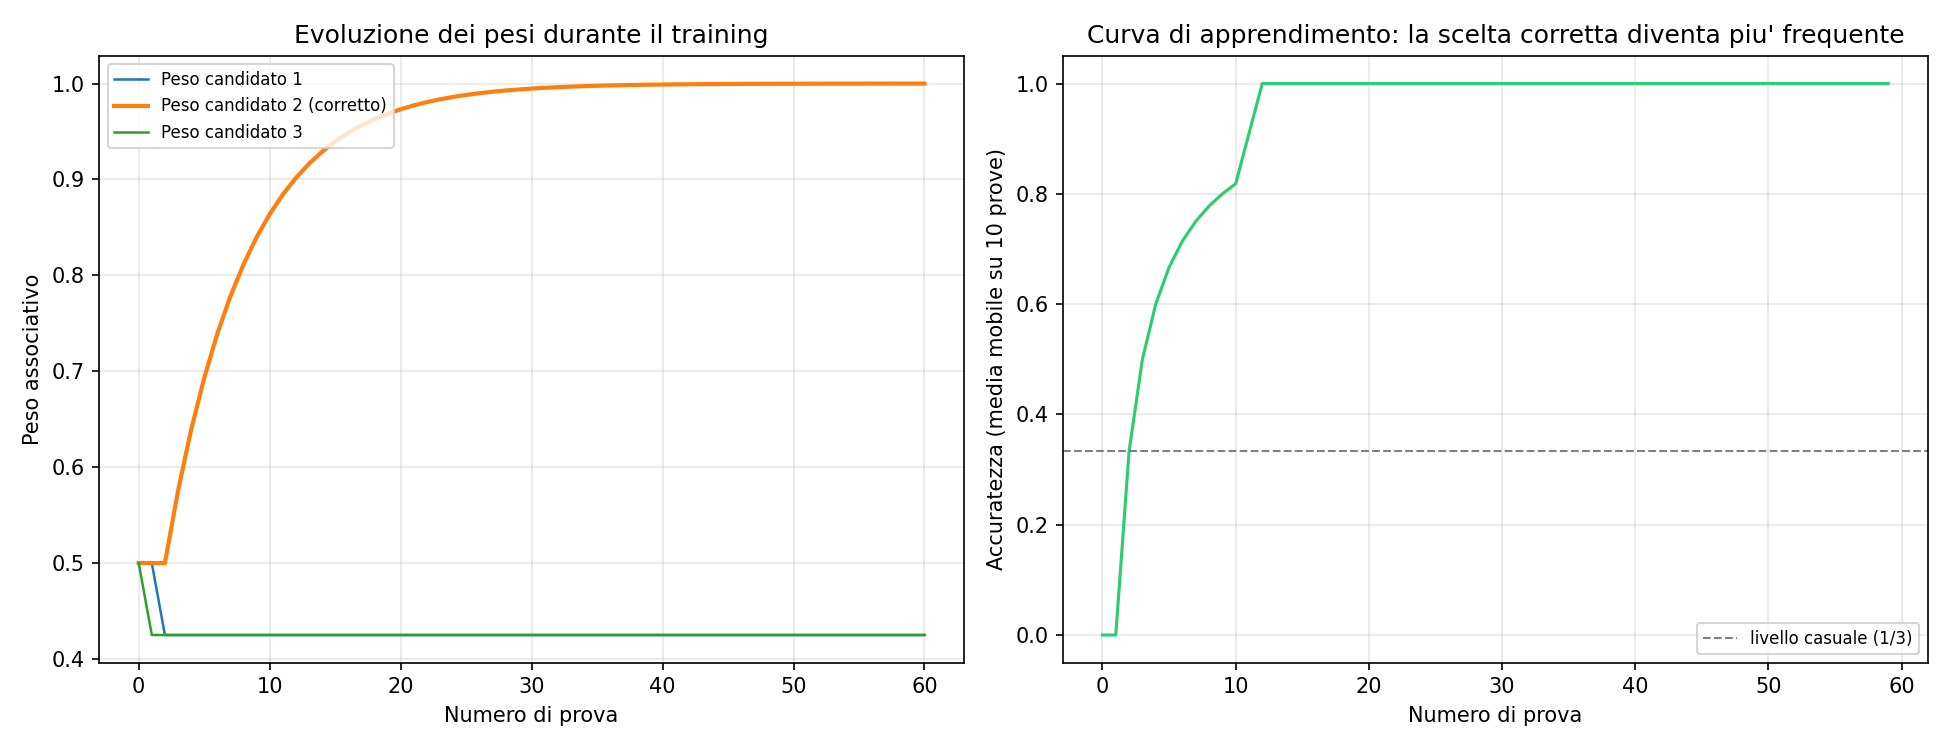
\includegraphics[width=6.3in,height=2.42308in]{media/media/image17.png}

\emph{Fig. 17 --- Evoluzione dei pesi durante il training (sinistra); curva di apprendimento dell\textquotesingle accuratezza (destra).}

\textit{\textbf{Codice sorgente: rl\_bandit.py}}

\lstinputlisting[language=Python]{scripts/rl_bandit.py}
\subsection{5.4 Politica contestuale: risposte diverse per contesti diversi}\label{politica-contestuale-risposte-diverse-per-contesti-diversi}

L\textquotesingle ultimo esperimento del progetto affronta un compito significativamente piu\textquotesingle{} difficile del bandito a tre braccia della sezione 5.3: invece di un\textquotesingle unica associazione corretta fissa da scoprire, la posizione dello stimolo su A definisce ora un CONTESTO tra tre possibili, e CIASCUN contesto ha una propria risposta corretta diversa dalle altre:

{\def\LTcaptype{none} % do not increment counter
\begin{longtable}[]{@{}
  >{\raggedright\arraybackslash}p{(\linewidth - 4\tabcolsep) * \real{0.3333}}
  >{\raggedright\arraybackslash}p{(\linewidth - 4\tabcolsep) * \real{0.3333}}
  >{\raggedright\arraybackslash}p{(\linewidth - 4\tabcolsep) * \real{0.3333}}@{}}
\toprule\noalign{}
\begin{minipage}[b]{\linewidth}\raggedright
\textbf{Contesto}
\end{minipage} & \begin{minipage}[b]{\linewidth}\raggedright
\textbf{Posizione stimolo su A}
\end{minipage} & \begin{minipage}[b]{\linewidth}\raggedright
\textbf{Risposta corretta}
\end{minipage} \\
\midrule\noalign{}
\endhead
\bottomrule\noalign{}
\endlastfoot
Contesto 1 & x=0.10 & Candidato 1 \\
Contesto 2 & x=0.50 & Candidato 2 \\
Contesto 3 & x=0.80 & Candidato 3 \\
\end{longtable}
}

Il sistema deve imparare TRE associazioni contemporaneamente, non una sola -\/- e, cosa piu\textquotesingle{} importante dal punto di vista concettuale, deve dimostrare di aver imparato a DISTINGUERE i contesti tra loro, non semplicemente a sviluppare una preferenza generica per un candidato a prescindere dal contesto presentato. Questo richiede un meccanismo diverso da un singolo vettore di pesi: una TABELLA di pesi indicizzata sia per contesto sia per candidato (pesi{[}contesto{]}{[}candidato{]}), una forma elementare di memoria associativa condizionata al contesto -\/- concettualmente il primo passo verso una vera politica decisionale (che sceglie l\textquotesingle azione in funzione dello STATO osservato, non sempre la stessa azione indipendentemente dallo stato).

Durante il training (150 prove totali, con il contesto scelto casualmente a ogni prova tra i tre possibili, cosi\textquotesingle{} che il sistema debba imparare tutte e tre le associazioni in parallelo e non in sequenza separata), solo la riga della tabella corrispondente al contesto effettivamente presentato viene aggiornata a ogni prova.

\textbf{Valutazione finale, con un test pulito senza ulteriore aggiornamento dei pesi (10 prove per ciascun contesto): tutti e tre i contesti hanno raggiunto un\textquotesingle accuratezza del 100\% sul proprio candidato corretto, con la tabella dei pesi finale che mostra una diagonale chiaramente dominante (i tre valori corrispondenti alle associazioni corrette, vicini a 1.0) rispetto a tutti gli altri elementi della tabella (rimasti vicini al valore iniziale di 0.5, o leggermente sotto).}

{\def\LTcaptype{none} % do not increment counter
\begin{longtable}[]{@{}
  >{\raggedright\arraybackslash}p{(\linewidth - 4\tabcolsep) * \real{0.3333}}
  >{\raggedright\arraybackslash}p{(\linewidth - 4\tabcolsep) * \real{0.3333}}
  >{\raggedright\arraybackslash}p{(\linewidth - 4\tabcolsep) * \real{0.3333}}@{}}
\toprule\noalign{}
\begin{minipage}[b]{\linewidth}\raggedright
\textbf{Contesto}
\end{minipage} & \begin{minipage}[b]{\linewidth}\raggedright
\textbf{Accuratezza finale}
\end{minipage} & \begin{minipage}[b]{\linewidth}\raggedright
\textbf{Pesi finali (candidato 1, 2, 3)}
\end{minipage} \\
\midrule\noalign{}
\endhead
\bottomrule\noalign{}
\endlastfoot
Contesto 1 (x=0.10) & 100\% & {[}1.000, 0.500, 0.500{]} \\
Contesto 2 (x=0.50) & 100\% & {[}0.500, 1.000, 0.500{]} \\
Contesto 3 (x=0.80) & 100\% & {[}0.425, 0.425, 1.000{]} \\
\end{longtable}
}

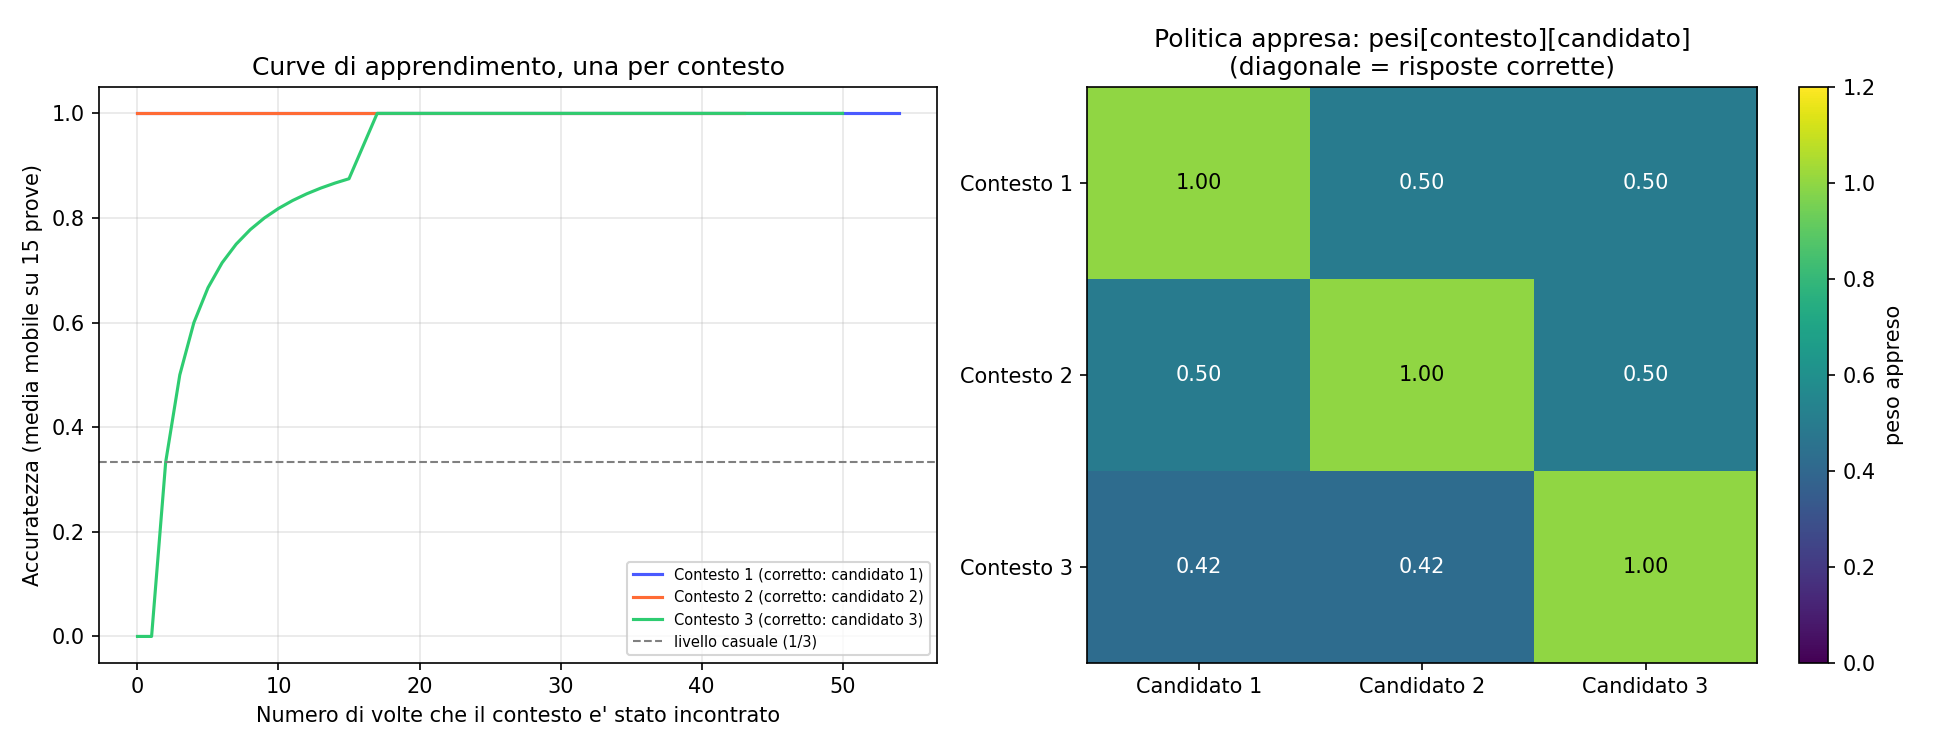
\includegraphics[width=6.3in,height=2.42308in]{media/media/image18.png}

\emph{Fig. 18 --- Curve di apprendimento per contesto (sinistra); politica finale appresa, tabella pesi{[}contesto{]}{[}candidato{]} (destra).}

\textbf{Perche\textquotesingle{} questo risultato e\textquotesingle{} concettualmente piu\textquotesingle{} avanzato del semplice bandito della sezione 5.3: un sistema che deve imparare una sola risposta corretta potrebbe, in linea di principio, "cavarsela" con una scorciatoia banale (una preferenza fissa, indipendente da qualunque informazione in ingresso). Un sistema che deve DISTINGUERE tra contesti diversi e rispondere in modo diverso a ciascuno non puo\textquotesingle{} ricorrere a questa scorciatoia -\/- deve necessariamente rappresentare, in qualche forma per quanto minimale (qui, la riga della tabella corrispondente), "in quale situazione mi trovo" prima di poter agire di conseguenza. E\textquotesingle, per quanto rudimentale nella sua realizzazione concreta, la differenza concettuale tra un riflesso fisso e l\textquotesingle inizio di una decisione condizionata al contesto osservato.}

\textit{\textbf{Codice sorgente: contextual\_policy.py}}

\lstinputlisting[language=Python]{scripts/contextual_policy.py}
\subsection{5.5 Comunicazione bidirezionale appresa: dal canale fisso alla sinapsi che impara}\label{comunicazione-bidirezionale-appresa-dal-canale-fisso-alla-sinapsi-che-impara}

La sezione 5.1 aveva costruito una catena A -\textgreater{} B a senso unico tra due ring attractor, con una mappa di proiezione (un offset fisso sull\textquotesingle anello) scritta a mano nel codice: B non aveva mai alcuna influenza su A. Questa sottosezione riprende esattamente quel punto e lo estende in due direzioni che il capitolo 9 elenca tra gli sviluppi futuri: rendere il canale bidirezionale, e rendere la mappa di proiezione una sinapsi vera, appresa invece che imposta dall\textquotesingle esterno. Il percorso, riportato per intero incluse le difficolta\textquotesingle{} incontrate (nello stesso spirito di trasparenza metodologica della sezione 4.4.1), attraversa quattro script successivi.

\subsubsection{5.5.1 Uno scambio a turni con canali fissi}\label{uno-scambio-a-turni-con-canali-fissi}

Primo passo, deliberatamente il piu\textquotesingle{} semplice possibile: due canali di proiezione fissi ma DIVERSI nelle due direzioni (A-\textgreater B con offset 0.3, B-\textgreater A con offset 0.2 -\/- con un\textquotesingle unica mappa uguale in entrambi i sensi lo scambio tornerebbe sempre allo stesso punto e non ci sarebbe nulla da osservare). I due ring si scambiano il turno esplicitamente invece di co-evolvere in continuo, altrimenti la dinamica converge quasi subito a un unico stato fuso.

Risultato: un messaggio iniziale su A genera uno scambio che NON converge a un punto fisso in 6 turni, ma oscilla. Lo spostamento netto per ogni andata-e-ritorno completo e\textquotesingle{} risultato empiricamente pari a circa 0.5 -\/- esattamente la somma dei due offset (0.3+0.2), confermando quantitativamente una predizione analitica invece di limitarsi a osservarla su un grafico. Un test di controllo (canale di ritorno disattivato) conferma che senza B-\textgreater A A resta ferma dopo un breve assestamento iniziale, coerente con il comportamento gia\textquotesingle{} documentato in 5.1.

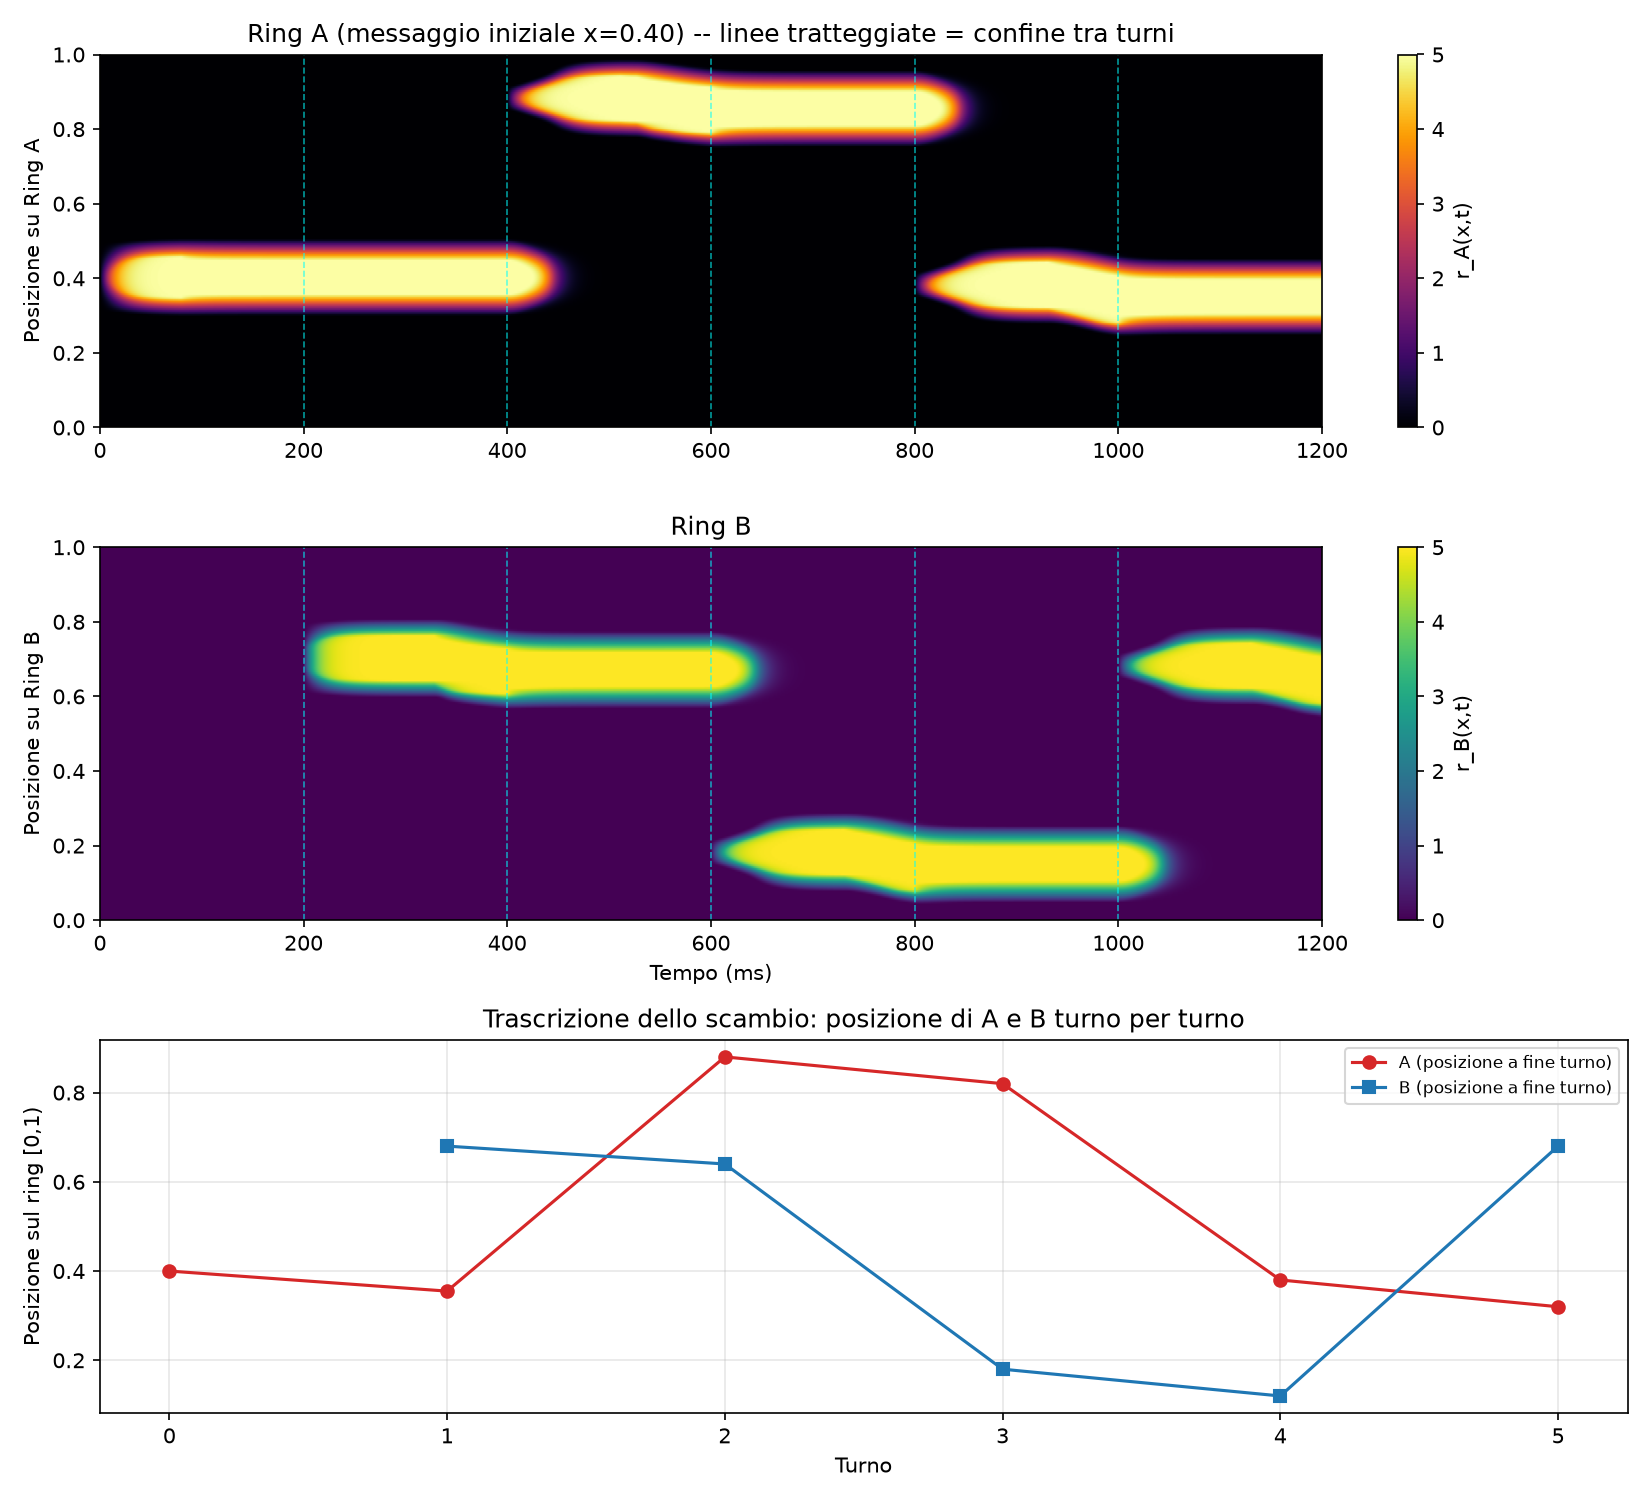
\includegraphics[width=5.8in,height=5.27273in]{media/media/image21.png}

\emph{Fig. 21 --- Scambio a turni con canali fissi: raster dei due ring e trascrizione posizione-per-turno.}

\textit{\textbf{Codice sorgente: dialogo\_ring\_attractor.py}}

\lstinputlisting[language=Python]{scripts/dialogo_ring_attractor.py}
\textit{\textbf{Codice sorgente: dialogo\_stdp.py}}

\lstinputlisting[language=Python]{scripts/dialogo_stdp.py}
\textit{\textbf{Codice sorgente: dialogo\_stdp\_adattamento.py}}

\lstinputlisting[language=Python]{scripts/dialogo_stdp_adattamento.py}
\textit{\textbf{Codice sorgente: dialogo\_multi\_messaggio.py}}

\lstinputlisting[language=Python]{scripts/dialogo_multi_messaggio.py}
\textit{\textbf{Codice sorgente: dialogo\_multi\_normalizzato.py}}

\lstinputlisting[language=Python]{scripts/dialogo_multi_normalizzato.py}
\textit{\textbf{Codice sorgente: dialogo\_multi\_repulsione.py}}

\lstinputlisting[language=Python]{scripts/dialogo_multi_repulsione.py}
\textit{\textbf{Codice sorgente: diagnosi\_bias\_posizione.py}}

\lstinputlisting[language=Python]{scripts/diagnosi_bias_posizione.py}
\textit{\textbf{Codice sorgente: dialogo\_multi\_repulsione\_3msg.py}}

\lstinputlisting[language=Python]{scripts/dialogo_multi_repulsione_3msg.py}
\textit{\textbf{Codice sorgente: dialogo\_multi\_scoperta\_locale.py}}

\lstinputlisting[language=Python]{scripts/dialogo_multi_scoperta_locale.py}
\textit{\textbf{Codice sorgente: dialogo\_multi\_scoperta\_locale\_montecarlo.py}}

\lstinputlisting[language=Python]{scripts/dialogo_multi_scoperta_locale_montecarlo.py}
\textit{\textbf{Codice sorgente: dialogo\_multi\_scoperta\_locale\_permutazione.py}}

\lstinputlisting[language=Python]{scripts/dialogo_multi_scoperta_locale_permutazione.py}
\textit{\textbf{Codice sorgente: dialogo\_multi\_scoperta\_locale\_mischiato.py}}

\lstinputlisting[language=Python]{scripts/dialogo_multi_scoperta_locale_mischiato.py}
\textit{\textbf{Codice sorgente: dialogo\_multi\_scoperta\_bidirezionale.py}}

\lstinputlisting[language=Python]{scripts/dialogo_multi_scoperta_bidirezionale.py}
\subsection{5.6 Verso il dominio spiking: un vero ring attractor a impulsi}\label{verso-il-dominio-spiking-un-vero-ring-attractor-a-impulsi}

Tutta la sezione 5.5 e\textquotesingle{} costruita su ring attractor a RATE (equazioni differenziali sul tasso di scarica, non su singoli impulsi) -\/- una scelta deliberata fin da ring\_attractor\_rate.py, fatta esplicitamente "per evitare i problemi di taratura della sincronia" degli attrattori spiking. Questa sezione affronta direttamente quel problema evitato: puo\textquotesingle{} un vero ring attractor a impulsi, con neuroni di Izhikevich identici a quelli usati in tutto il resto del progetto, sostenere un bump di attivita\textquotesingle{} localizzato e persistente?

Architettura: popolazione eccitatoria E (100 neuroni) disposta su un anello, con connettivita\textquotesingle{} E-\textgreater E a caduta gaussiana sulla distanza circolare (stessa larghezza sigma=0.05 del modello a rate) TAGLIATA nettamente oltre 3 deviazioni standard -\/- nessuna coda a lungo raggio. Popolazione inibitoria I (25 neuroni) condivisa e non spazializzata, connettivita\textquotesingle{} casuale sparsa (stesso stile di rete\_300\_neuroni.py), per l\textquotesingle inibizione globale che sopprime l\textquotesingle attivita\textquotesingle{} lontano dal bump.

Il percorso di tuning, riportato per intero nello stesso spirito di trasparenza metodologica della sezione 4.4.1: dieci tentativi successivi. Sinapsi E-\textgreater E istantanee (un salto di potenziale ad ogni spike, come in tutto il resto del progetto) non hanno mai funzionato -\/- o non bastavano a formare un bump (pesi deboli), o lo facevano propagare a tutto l\textquotesingle anello come un\textquotesingle onda viaggiante o una vera e propria crisi epilettiforme (pesi forti, fino a 650 Hz di picco di popolazione seguiti da silenzio totale per adattamento). La svolta e\textquotesingle{} arrivata sostituendo la componente E-\textgreater E con una corrente LENTA in stile NMDA (costante di tempo 100ms, Compte et al. 2000 / Wang 2002) invece del salto istantaneo -\/- integra molti impulsi nel tempo invece di dare uno scatto che innesca instabilita\textquotesingle{} veloci. Da li\textquotesingle, altri quattro tentativi per ritarare inibizione e rumore di fondo attorno alla nuova dinamica piu\textquotesingle{} lenta, fino a un vero punto di equilibrio.

Risultato finale, verificato su due finestre temporali distanziate (460-660ms e 900-1100ms dopo la rimozione dello stimolo, non solo una singola misura) per distinguere un vero equilibrio da una lenta deriva: 154 spike nella finestra precoce contro 147 nella finestra tardiva (variazione -5\%), larghezza spaziale del bump quasi identica (0.058 contro 0.063). Il bump resta localizzato nella stessa banda stretta dell\textquotesingle anello per quasi 900ms dopo la rimozione dello stimolo, senza spegnersi ne\textquotesingle{} diffondersi al resto della popolazione. Il centro stimato si discosta dal centro dello stimolo di \textasciitilde0.03-0.05 unita\textquotesingle{} -\/- coerente con lo stesso ordine di grandezza del bias di posizione gia\textquotesingle{} documentato per il ring attractor a rate (sezioni 4.4.2, 5.1, 5.2, 8), un\textquotesingle indicazione che il fenomeno potrebbe non essere specifico del modello a rate ma una proprieta\textquotesingle{} piu\textquotesingle{} generale di questa classe di attrattori discretizzati.

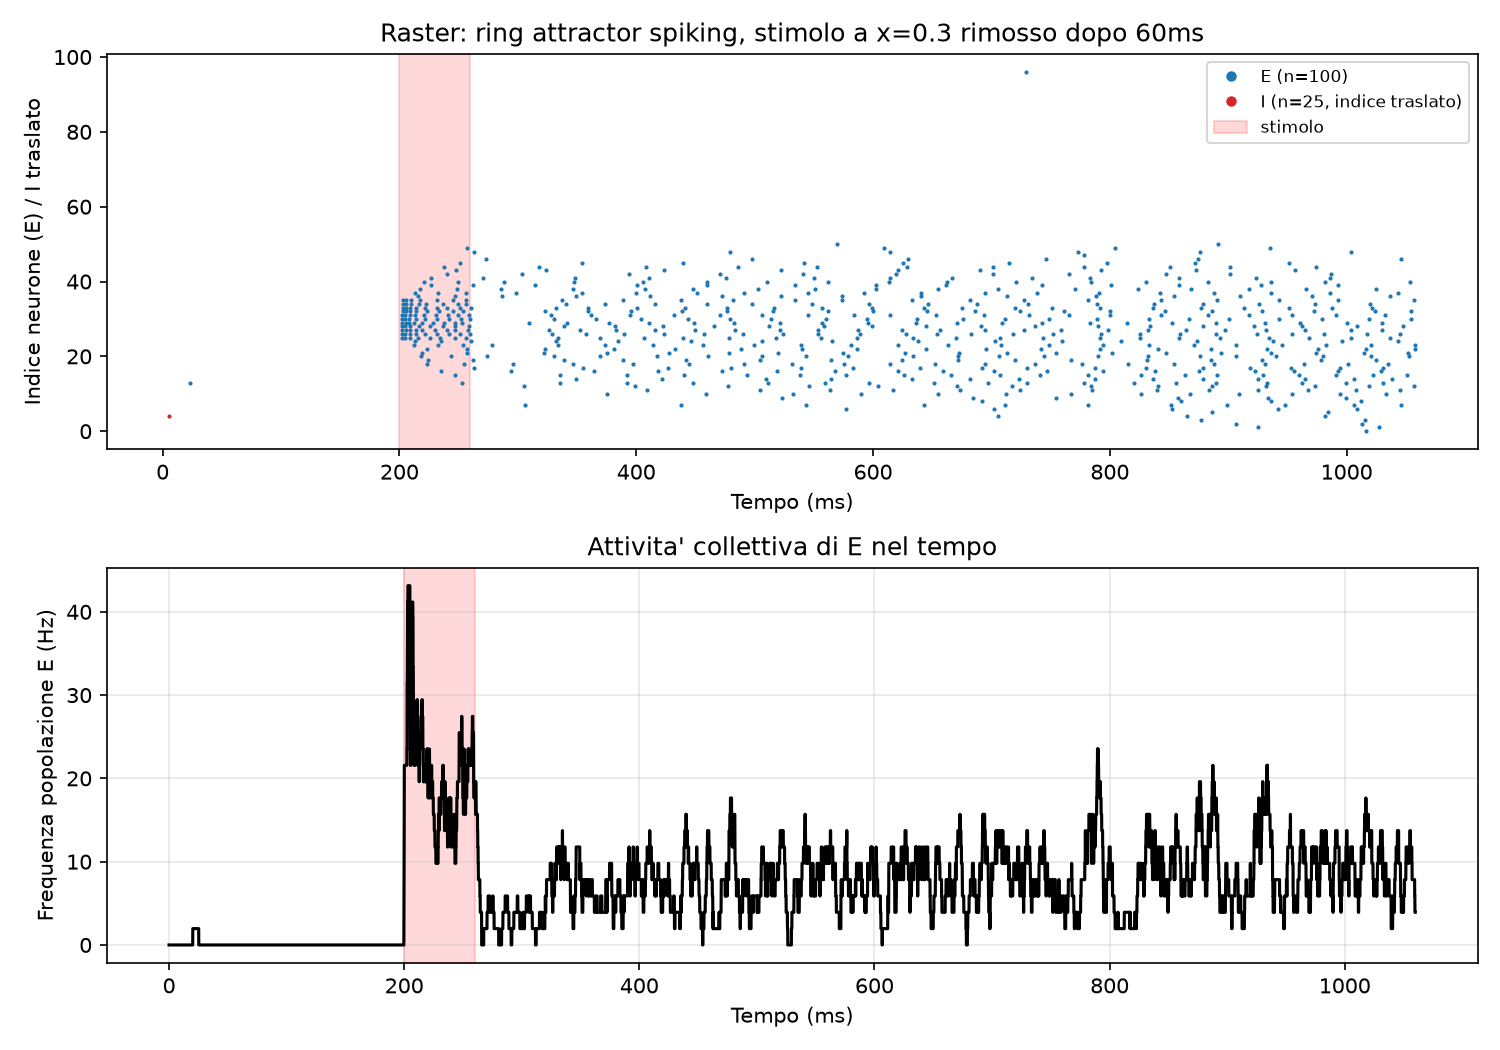
\includegraphics[width=5.8in,height=4.06in]{media/media/image34.png}

\emph{Fig. 33 --- Ring attractor spiking: raster e frequenza di popolazione. Il bump (indici \textasciitilde15-40) resta localizzato e persistente per quasi 900ms dopo la rimozione dello stimolo (a 260ms).}

\textit{\textbf{Codice sorgente: ring\_attractor\_spiking.py}}

\lstinputlisting[language=Python]{scripts/ring_attractor_spiking.py}
\subsection{5.7 Comunicazione appresa tra due anelli spiking, con STDP vera}\label{comunicazione-appresa-tra-due-anelli-spiking-con-stdp-vera}

Con un ring attractor spiking stabile disponibile (sezione 5.6), il passo naturale successivo e\textquotesingle{} collegarne due con una sinapsi che impara -\/- ma questa volta con STDP autentica, basata sui tempi di spike reali (Song \& Abbott 2001, lo stesso schema di stdp.py), non piu\textquotesingle{} l\textquotesingle approssimazione Hebbiana a grana di turno usata in tutta la sezione 5.5. Si comincia da un solo verso (A-\textgreater B), come il progetto ha sempre fatto nel dominio a rate.

Primo ostacolo, diverso da qualunque cosa incontrata nel modello a rate: un vero cortocircuito uovo-gallina strutturale. B, da solo, non si accende mai spontaneamente (verificato in 5.6: il rumore di fondo non basta a innescare un bump, serve una spinta esterna netta). Senza che B spari MAI, non esiste alcuno spike "post" con cui la STDP possa accoppiare gli spike "pre" di A -\/- la regola di apprendimento non ha mai un segnale da cui imparare. Risolto alzando peso iniziale e densita\textquotesingle{} delle sinapsi inter-anello abbastanza da garantire che i primi tentativi accendano davvero B almeno qualche volta.

Secondo ostacolo: con connettivita\textquotesingle{} inter-anello UNIFORME (ogni neurone di A collegato a caso a neuroni di B su tutto l\textquotesingle anello), la risposta di B risultava diffusa su tutta la popolazione invece che localizzata -\/- nessuna struttura spaziale su cui la dinamica propria di B (eccitazione locale, inibizione globale) potesse concentrarsi. Risolto dando alla connettivita\textquotesingle{} iniziale A-\textgreater B una debole caduta gaussiana sulla distanza circolare (offset zero, l\textquotesingle analogo spiking di un bias innato "identita\textquotesingle") -\/- lo stesso principio, gia\textquotesingle{} verificato nel modello a rate, che un debole ordine di partenza sulla struttura spaziale e\textquotesingle{} necessario perche\textquotesingle{} la scoperta STDP abbia qualcosa di coerente su cui costruire.

Risultato, su 60 ripetizioni dello stesso messaggio (stimolo su A a x=0.3, 24 secondi di simulazione continua): la risposta di B resta localizzata nella posizione corretta per l\textquotesingle intera durata (centro stimato 0.301 nelle prime 5 ripetizioni, 0.306 nelle ultime 5 -\/- praticamente identico allo stimolo, senza la deriva vista nei primi tentativi) e si RAFFORZA nel tempo (21 spike di B nelle prime 5 ripetizioni, 44 nelle ultime 5). I pesi delle sinapsi A-\textgreater B crescono genuinamente tramite la regola STDP (picco massimo da 1.5mV a 3.6mV), non per un meccanismo esterno imposto. E\textquotesingle{} la prima dimostrazione, in questo progetto, di comunicazione appresa tra due popolazioni spiking con plasticita\textquotesingle{} sinaptica autentica basata sui tempi di spike.

Non ancora tentato in questo lavoro: la bidirezionalita\textquotesingle{} (canale di ritorno B-\textgreater A, con la stessa asimmetria strutturale gia\textquotesingle{} affrontata nella sezione 5.5.3 -\/- probabilmente accentuata qui dal fatto che A, come B, e\textquotesingle{} un vero attrattore che una volta acceso non si spegne facilmente) e il test con piu\textquotesingle{} messaggi (l\textquotesingle interferenza gia\textquotesingle{} affrontata nella sezione 5.5.6 in avanti, qui con la complicazione aggiuntiva che la connettivita\textquotesingle{} inter-anello spaziale usata per bootstrappare un messaggio potrebbe non generalizzare automaticamente a messaggi diversi). Lasciati come sviluppi futuri.

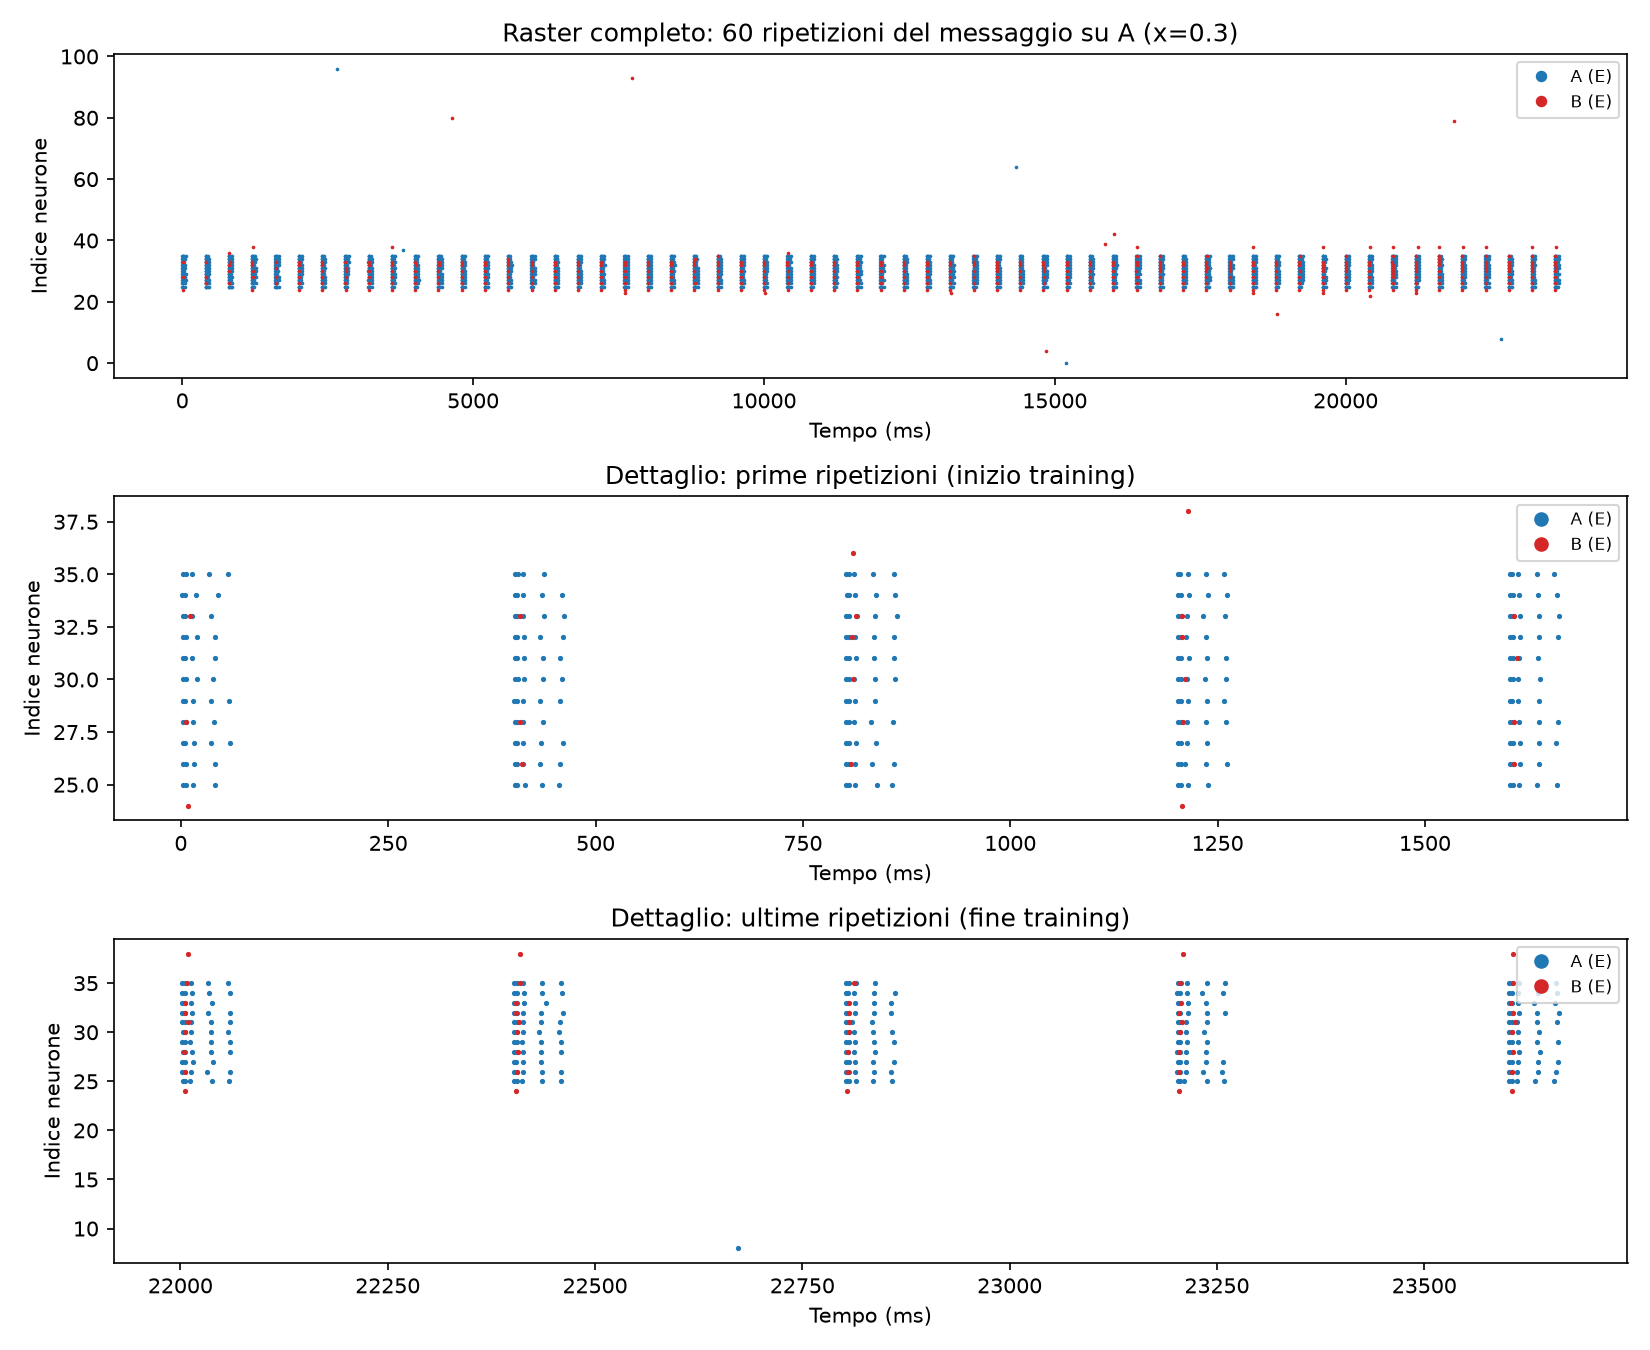
\includegraphics[width=5.8in,height=4.74545in]{media/media/image35.png}

\emph{Fig. 34 --- Comunicazione appresa A-\textgreater B con STDP vera: raster completo (60 ripetizioni) e dettaglio inizio/fine training. La risposta di B resta localizzata e si rafforza nel tempo.}

\textit{\textbf{Codice sorgente: dialogo\_spiking.py}}

\lstinputlisting[language=Python]{scripts/dialogo_spiking.py}
\subsection{5.8 Tentativo di bidirezionalita\textquotesingle{} spiking: la stessa asimmetria del modello a rate}\label{tentativo-di-bidirezionalita-spiking-la-stessa-asimmetria-del-modello-a-rate}

Estensione diretta di dialogo\_spiking.py: stessa architettura, stessa connettivita\textquotesingle{} inter-anello a caduta gaussiana, aggiunta pero\textquotesingle{} anche nel verso B-\textgreater A (STDP vera su entrambi i canali). L\textquotesingle aspettativa, dichiarata esplicitamente prima di eseguire il test, era che si presentasse lo stesso ostacolo gia\textquotesingle{} incontrato e risolto nel modello a rate (sezione 5.5.3): A e\textquotesingle{} un attrattore che, una volta acceso dallo stimolo diretto, non si spegne da solo (verificato in 5.6, persistenza per quasi 900ms) -\/- B deve quindi competere con un bump gia\textquotesingle{} a piena potenza invece di accenderne uno da zero, un compito molto piu\textquotesingle{} difficile.

Risultato su 60 ripetizioni, stessa configurazione di 5.7: il canale A-\textgreater B continua a funzionare bene (28 spike di B nelle prime 5 ripetizioni, 50 nelle ultime, centro stabile a x=0.30-0.31). Il canale B-\textgreater A pero\textquotesingle{} non mostra alcun segnale di apprendimento utile -\/- il peso medio resta sostanzialmente invariato (1.500mV iniziale, 1.471mV finale, una leggera diminuzione netta: mix di potenziamento e depressione che si annullano quasi del tutto), e zero spike di A oltre la finestra direttamente spiegabile dallo stimolo esterno, sia all\textquotesingle inizio sia alla fine del training -\/- nessuna evidenza che B abbia mai influenzato A in un solo caso sulle 60 ripetizioni.

L\textquotesingle ipotesi dichiarata in apertura e\textquotesingle{} confermata: la stessa asimmetria strutturale del modello a rate si ripresenta identica nel dominio spiking. La correzione che ha funzionato li\textquotesingle{} -\/- adattamento a soglia di scarica piu\textquotesingle{} uno schema a turni con pause di silenzio (sezione 5.5.3) -\/- richiederebbe qui un lavoro di calibrazione comparabile a quello gia\textquotesingle{} fatto per l\textquotesingle attrattore singolo (sezione 5.6, dieci tentativi): un vero meccanismo di adattamento per far si\textquotesingle{} che anche A si affievolisca senza nuovo stimolo esterno, e uno schema di stimolo periodico con finestre di vero silenzio invece della ripetizione continua usata qui. Non tentato in questa sessione per limiti di tempo -\/- lasciato come sviluppo futuro, documentato onestamente come risultato negativo atteso e confermato, non come un fallimento nascosto.

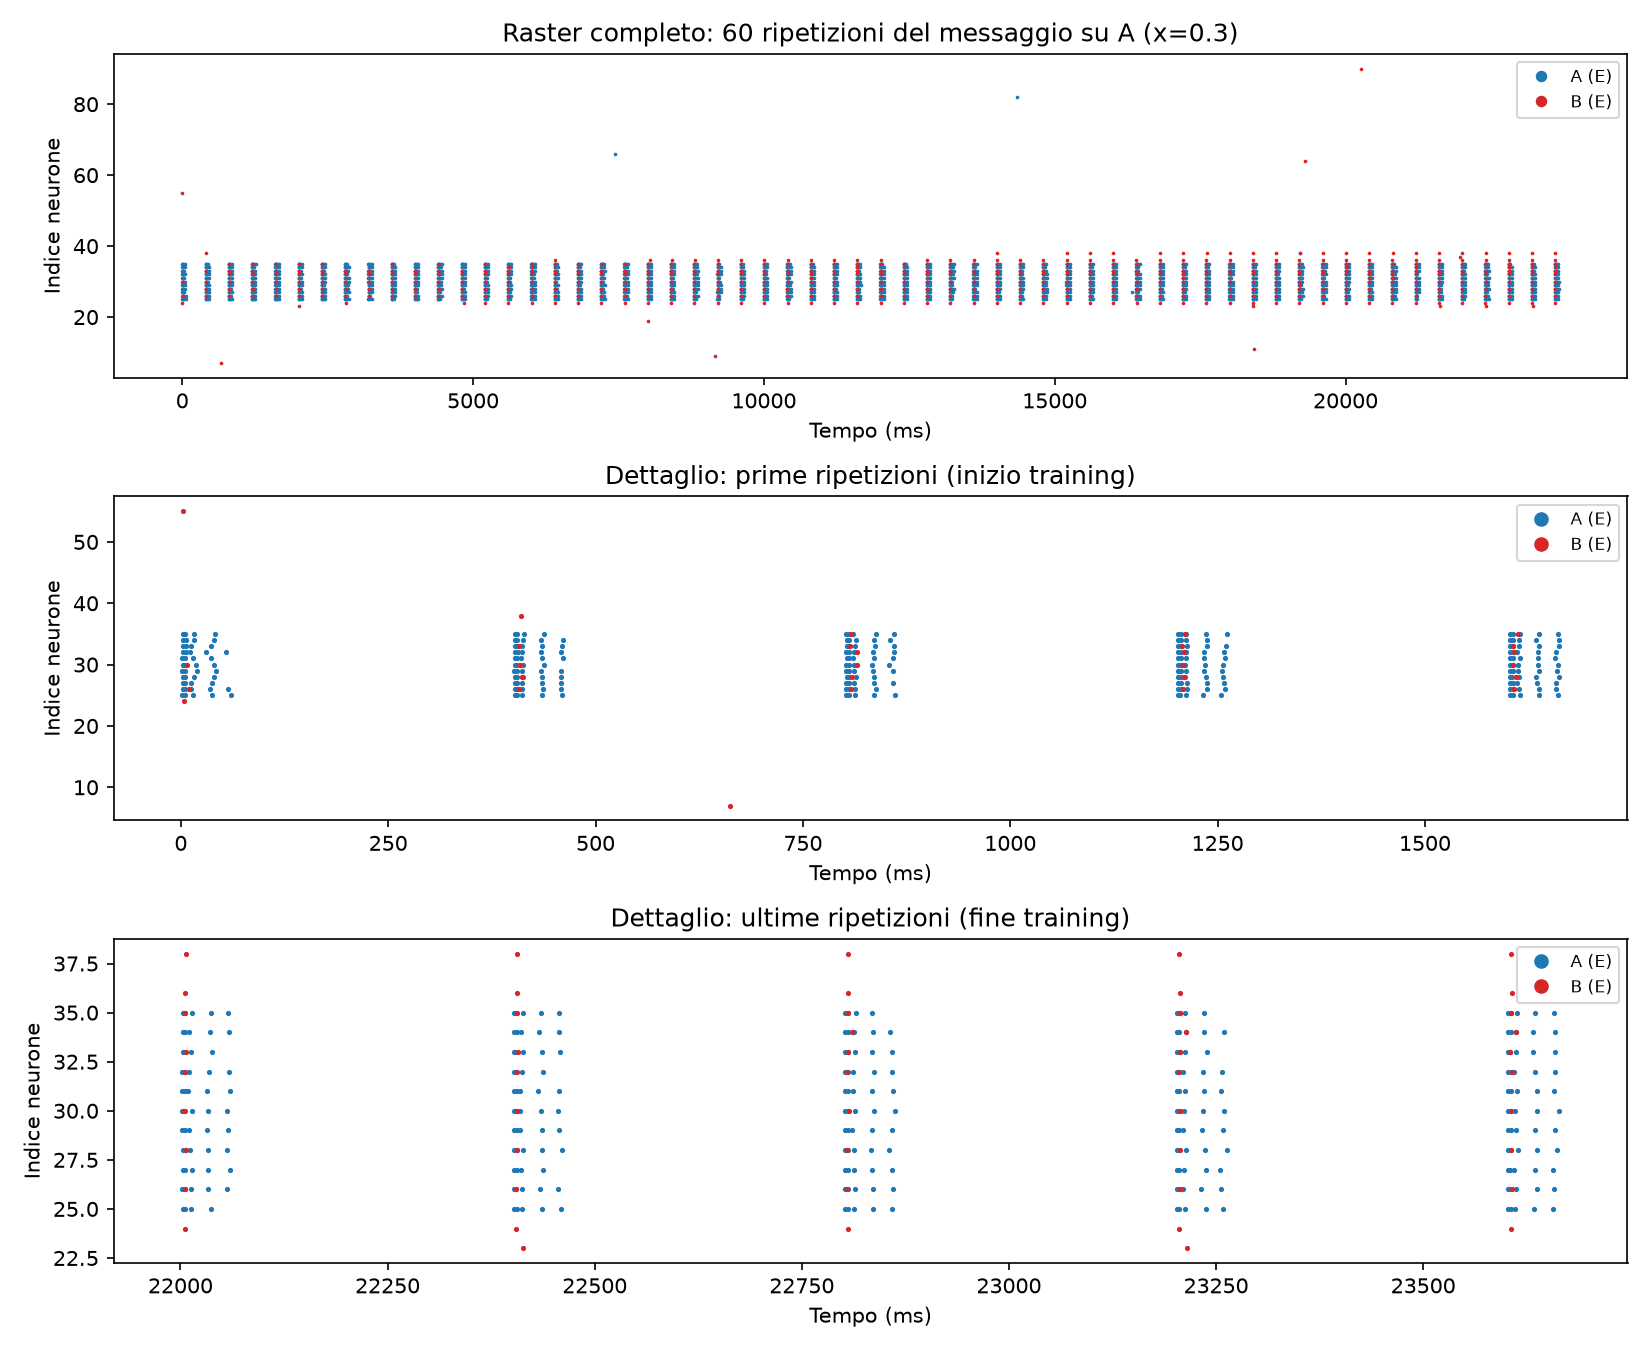
\includegraphics[width=5.8in,height=4.74545in]{media/media/image36.png}

\emph{Fig. 35 --- Tentativo di bidirezionalita\textquotesingle{} spiking: A-\textgreater B continua a funzionare, B-\textgreater A non mostra segnale di apprendimento in nessuna delle 60 ripetizioni.}

\textit{\textbf{Codice sorgente: dialogo\_spiking\_bidirezionale.py}}

\lstinputlisting[language=Python]{scripts/dialogo_spiking_bidirezionale.py}
\subsection{5.9 Bidirezionalita\textquotesingle{} spiking: isolamento del confondimento e conclusione negativa definitiva}\label{bidirezionalita-spiking-isolamento-del-confondimento-e-conclusione-negativa-definitiva}

Seguito diretto della sezione 5.8. Due correzioni via via piu\textquotesingle{} forti sono state provate prima di arrivare a una conclusione solida: aggiungere adattamento di popolazione su entrambi gli anelli (perche\textquotesingle{} A si affievolisca da solo, come nella correzione 5.5.3 del modello a rate) e, in un tentativo successivo, aumentare peso iniziale e tetto delle sinapsi inter-anello (w\_init 1.5mV-\textgreater3.5mV, w\_max 5.0mV-\textgreater8.0mV) per spingere B oltre la soglia di un\textquotesingle ignizione autosufficiente. Risultato di questi due tentativi: la risposta di B si e\textquotesingle{} rafforzata parecchio (fino a 247 spike per finestra, contro i 21-44 della sezione 5.7), e il peso medio B-\textgreater A e\textquotesingle{} cresciuto fino a toccare il tetto -\/- ma il conteggio di spike di A oltre 20ms dopo la fine dello stimolo esterno e\textquotesingle{} rimasto a zero o quasi in ogni caso. Il raster ha mostrato perche\textquotesingle: A e B sparano nello stesso brevissimo burst di 60-80ms, sempre in coincidenza con lo stimolo diretto su A -\/- non due eventi separati nel tempo.

Primo tentativo di isolamento (dialogo\_spiking\_bidirezionale\_turni.py): invece di stimolare sempre A, lo stimolo esterno diretto alterna tra anelli, un turno \textquotesingle A\textquotesingle{} e un turno \textquotesingle B\textquotesingle{} (sulla stessa posizione), separati da una pausa piena di 940ms. Nei turni \textquotesingle B\textquotesingle, A non riceve alcuno stimolo diretto: qualunque suo spike deve passare per forza dalla sinapsi appresa B-\textgreater A. Risultato: zero spike di A durante i turni \textquotesingle B\textquotesingle{} in ogni fase del training (0 all\textquotesingle inizio, 0 alla fine) -\/- eppure il peso medio B-\textgreater A continuava comunque a crescere fino al tetto. La spiegazione trovata analizzando i cicli: durante i turni \textquotesingle A\textquotesingle, B risponde ormai cosi\textquotesingle{} rapidamente (decine di ms) che A e B finiscono per sparare quasi insieme anche in quei turni, e la regola STDP sul canale B-\textgreater A non puo\textquotesingle{} distinguere questa coincidenza da una vera causalita\textquotesingle{} B-\textgreater A.

Correzione chirurgica (dialogo\_spiking\_bidirezionale\_gate.py): plasticita\textquotesingle{} del canale B-\textgreater A disattivata (tramite una variabile "shared" ltp\_gate/ltd\_gate, azzerata e ripristinata tra un turno e l\textquotesingle altro) durante i turni \textquotesingle A\textquotesingle{} -\/- la trasmissione resta sempre attiva, solo l\textquotesingle aggiornamento del peso viene bloccato quando la coincidenza e\textquotesingle{} possibile. Il canale B-\textgreater A puo\textquotesingle{} cosi\textquotesingle{} imparare ESCLUSIVAMENTE nei turni in cui non esiste alcuna possibilita\textquotesingle{} di confondimento. Risultato, ripetuto su due run indipendenti: il peso medio B-\textgreater A resta sostanzialmente piatto (3.500mV iniziale, 3.511mV e 3.506mV finale nei due run, contro il +0.257mV del tentativo senza gating) e il numero di spike di A durante i turni \textquotesingle B\textquotesingle{} resta a 0-2 per finestra di 5 turni, senza localizzazione consistente sulla posizione del messaggio tra un run e l\textquotesingle altro (un run da\textquotesingle{} un piccolo gruppo di 6 spike esattamente a x=0.300 nelle ultime ripetizioni; il run indipendente successivo ne da\textquotesingle{} invece 2 a x=0.170, un\textquotesingle altra posizione) -\/- il segno di un fluttuazione di rumore di fondo, non di un segnale riproducibile.

Conclusione: con il confondimento eliminato alla radice, il canale di ritorno B-\textgreater A non mostra alcuna evidenza di trasmissione causale reale in questo sistema. La crescita di peso osservata in tutti i tentativi precedenti (5.8 e i primi due di questa sezione) era interamente spiegabile dalla coincidenza temporale tra la risposta di B e lo stimolo diretto su A, non da un vero apprendimento del canale di ritorno. A differenza del modello a rate (dove la sezione 5.5.3 ha risolto lo stesso problema strutturale), nel dominio spiking l\textquotesingle adattamento e il rinforzo dei pesi non bastano: il vincolo piu\textquotesingle{} stringente e\textquotesingle{} che, con una connettivita\textquotesingle{} inter-anello abbastanza forte da far rispondere B in modo affidabile, la latenza di quella risposta e\textquotesingle{} troppo breve rispetto alla finestra della regola STDP per generare mai un segnale pre/post scorrelato dallo stimolo diretto -\/- un vincolo temporale specifico del dominio spiking, senza equivalente diretto nell\textquotesingle approssimazione a turni del modello a rate.

Nota onesta su un\textquotesingle osservazione minore, controllata e non invalidante: nel secondo run con gating, dopo circa 36 secondi di simulazione continua compare, in entrambi gli anelli quasi nello stesso istante (t=38017.7ms in A, t=38018.8ms in B), un piccolo gruppo di spike vicino al bordo dell\textquotesingle anello (indice \textgreater=90, x\textgreater=0.90, prossimo al punto di raccordo x=1.0-\textgreater0.0). Verificato sui dati grezzi degli spike: si tratta di 30 spike in A e 16 in B su un totale di circa 1750 spike per anello dopo quel momento (meno del 2\%), non di una banda persistente per tutto il resto della simulazione come sembrava a un primo sguardo sul raster a scala intera (un effetto ottico dei marcatori piccoli su 60 secondi di grafico). L\textquotesingle ipotesi piu\textquotesingle{} plausibile e\textquotesingle{} una singola co-ignizione spontanea innescata dal rumore di fondo, resa possibile a quel punto del training dal fatto che molte sinapsi inter-anello erano ormai vicine al tetto di 8.0mV. Non e\textquotesingle{} stata approfondita oltre: non altera il conteggio dominante usato per la valutazione (basato su migliaia di spike nel pattern localizzato consueto), ma e\textquotesingle{} un promemoria che le simulazioni continue molto lunghe su attrattori NMDA-sostenuti possono, in rari casi, generare accensioni spontanee secondarie non legate allo stimolo.

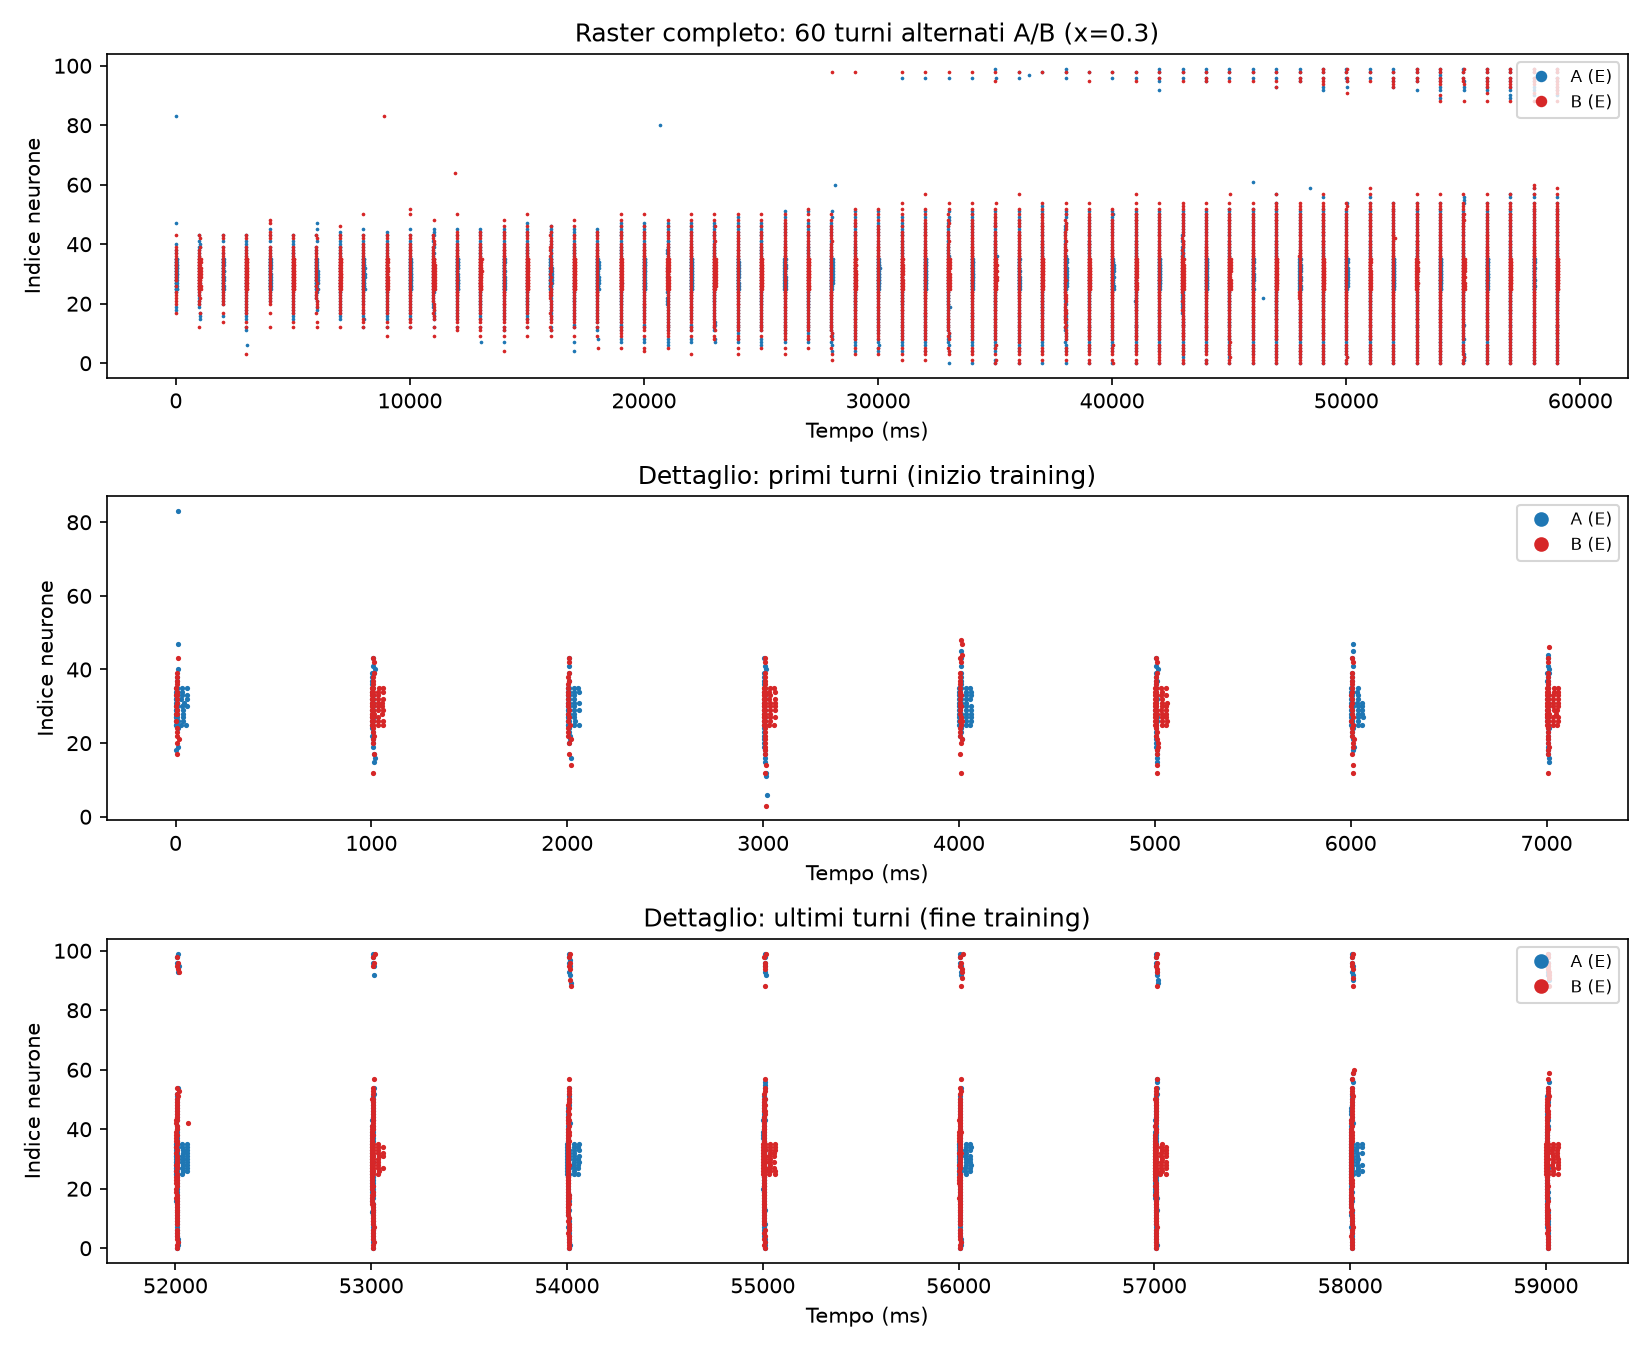
\includegraphics[width=5.8in,height=4.74545in]{media/media/image37.png}

\emph{Fig. 36 --- Schema a turni A/B: isola il confondimento ma il peso B-\textgreater A continua a crescere per coincidenza durante i turni \textquotesingle A\textquotesingle.}

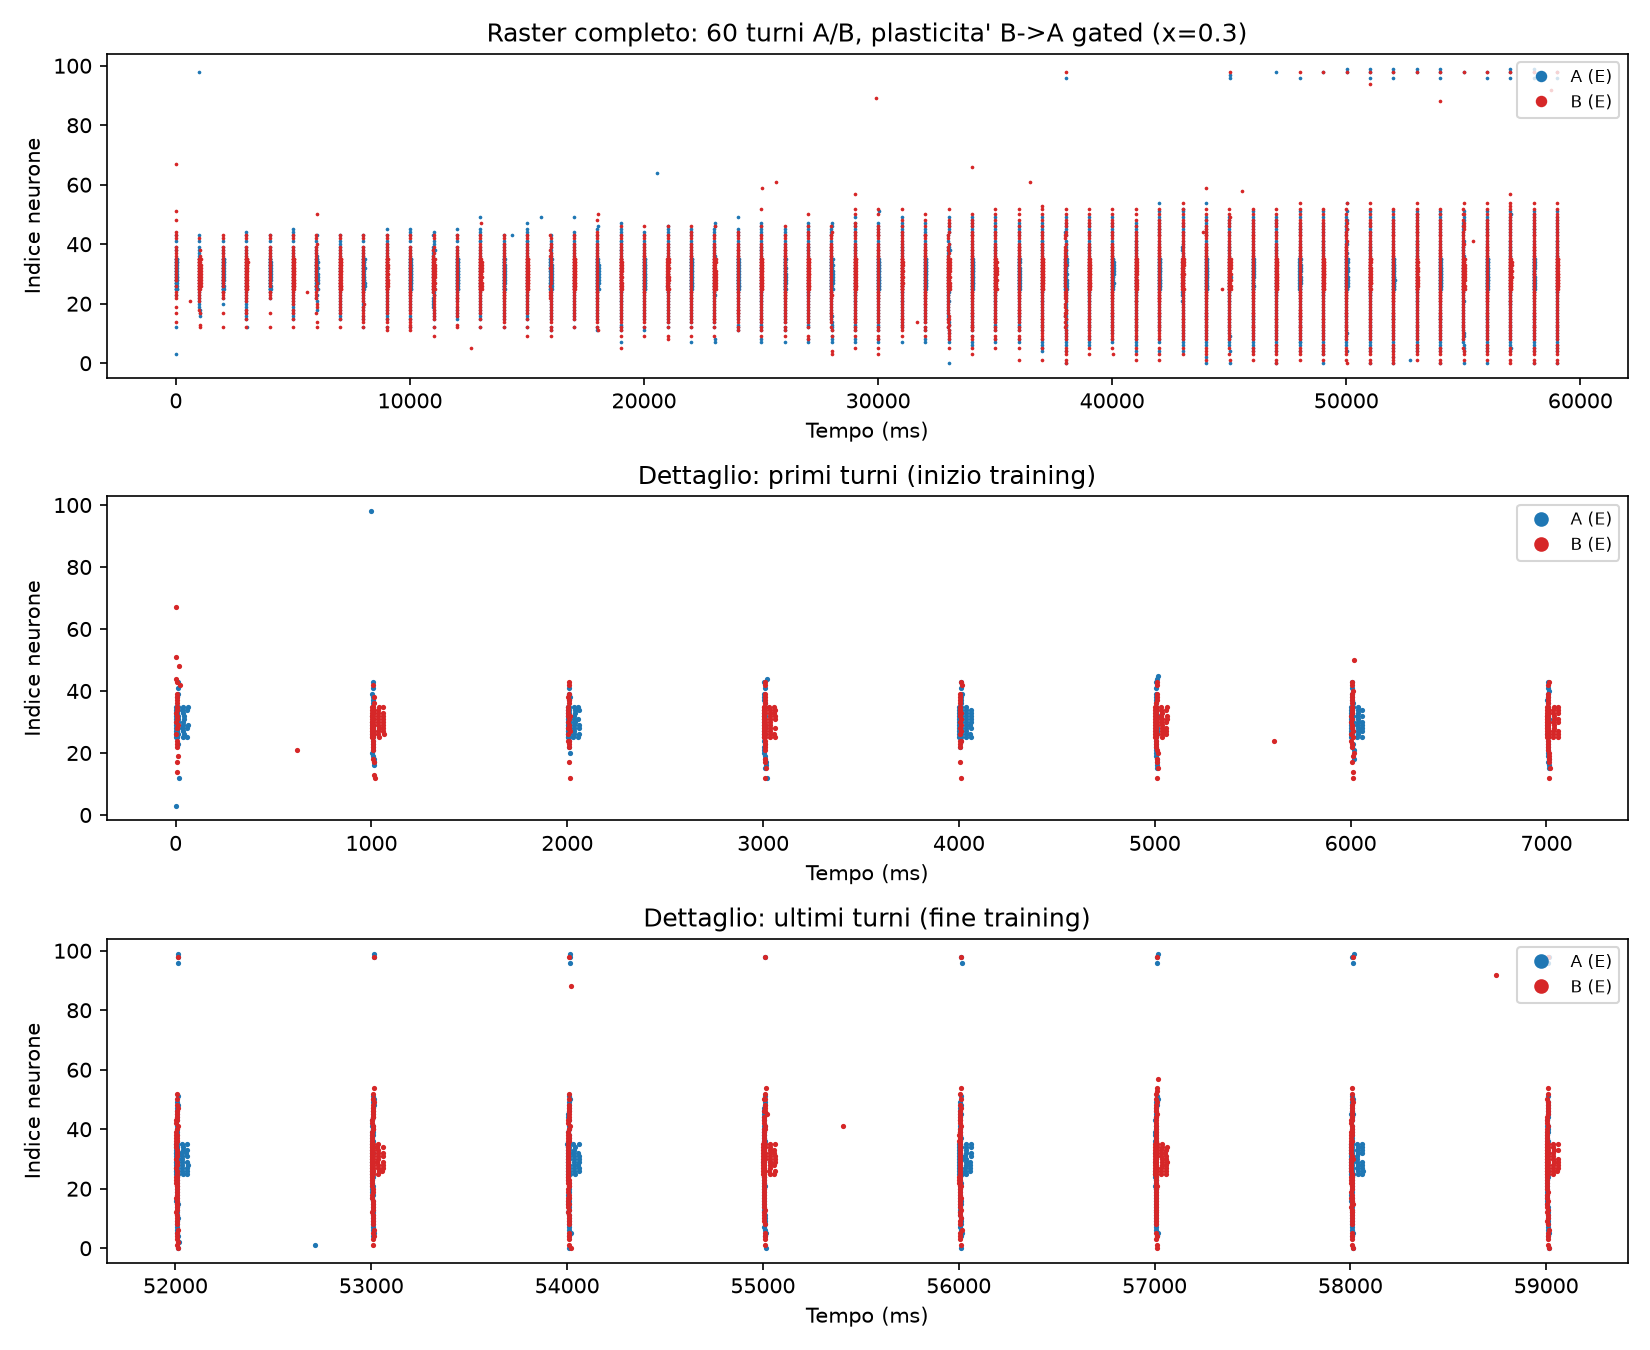
\includegraphics[width=5.8in,height=4.74545in]{media/media/image38.png}

\emph{Fig. 37 --- Schema a turni con plasticita\textquotesingle{} B-\textgreater A disattivata durante i turni \textquotesingle A\textquotesingle: il peso resta piatto, conclusione negativa pulita.}

\textit{\textbf{Codice sorgente: dialogo\_spiking\_bidirezionale\_turni.py}}

\lstinputlisting[language=Python]{scripts/dialogo_spiking_bidirezionale_turni.py}
\textit{\textbf{Codice sorgente: dialogo\_spiking\_bidirezionale\_gate.py}}

\lstinputlisting[language=Python]{scripts/dialogo_spiking_bidirezionale_gate.py}
\subsection{5.10 Piu\textquotesingle{} messaggi in dominio spiking: nessuna interferenza, a differenza del modello a rate}\label{piu-messaggi-in-dominio-spiking-nessuna-interferenza-a-differenza-del-modello-a-rate}

Ultimo sviluppo segnalato come lavoro futuro nella sezione 5.7: estendere la comunicazione appresa A-\textgreater B (STDP vera) a piu\textquotesingle{} di un messaggio. Stesse due posizioni usate nel primo test di interferenza del modello a rate (dialogo\_multi\_messaggio.py, sezione 5.5.4): x=0.15 e x=0.65, allenate in alternanza round-robin (30 ripetizioni ciascuna, 60 totali).

Ipotesi dichiarata prima di eseguire il test: nel modello a rate l\textquotesingle interferenza nasceva dal fatto che i pesi inter-popolazione partivano CASUALI, e ogni messaggio doveva attraversare un vero processo di scoperta (prima rumore puro, poi rumore con repulsione, poi scoperta locale, sezioni 5.5.4-5.5.9) per trovare la propria mappa in uno spazio di pesi condiviso -\/- da cui la competizione quando due scoperte avvenivano nello stesso spazio. Nel dominio spiking, invece, la connettivita\textquotesingle{} inter-anello parte gia\textquotesingle{} strutturata (caduta gaussiana sulla distanza circolare, offset zero, sezione 5.7): la mappa identita\textquotesingle{} esiste prima ancora che la STDP cominci ad allenare qualunque cosa. Non essendoci alcun processo di scoperta condiviso, il meccanismo che causava l\textquotesingle interferenza nel modello a rate potrebbe semplicemente non avere un equivalente qui.

Risultato: l\textquotesingle ipotesi si conferma pienamente. Entrambi i messaggi si rafforzano nel corso del training (x=0.15: 28-\textgreater45 spike di B tra prime e ultime 5 ripetizioni; x=0.65: 17-\textgreater38 spike) e restano localizzati con precisione per tutta la durata (errore rispetto alla posizione del messaggio: 0.004-\textgreater0.016 per x=0.15, 0.026-\textgreater0.001 per x=0.65 -\/- in entrambi i casi ben al di sotto della larghezza dello stimolo, 0.05). Il raster mostra due bande nettamente separate e stabili (indici 10-20 e 60-70) per l\textquotesingle intera simulazione di 24 secondi, senza alcuna deriva ne\textquotesingle{} contaminazione incrociata tra le due -\/- nessuna traccia della competizione osservata nel modello a rate.

Interpretazione: la differenza cruciale non e\textquotesingle{} il dominio (spiking contro rate) in se\textquotesingle, ma la presenza o assenza di un processo di scoperta condiviso. L\textquotesingle interferenza nel modello a rate non era una proprieta\textquotesingle{} intrinseca della comunicazione tra due popolazioni, ma una conseguenza specifica di come i pesi venivano inizializzati e allenati la\textquotesingle{} -\/- una conclusione che rafforza retroattivamente l\textquotesingle interpretazione data in sezione 5.5.7 (l\textquotesingle ipotesi del bias di posizione come causa dell\textquotesingle interferenza era stata refutata direttamente; qui si osserva il caso complementare, un sistema senza il meccanismo di scoperta condiviso che semplicemente non presenta interferenza fin dall\textquotesingle inizio).

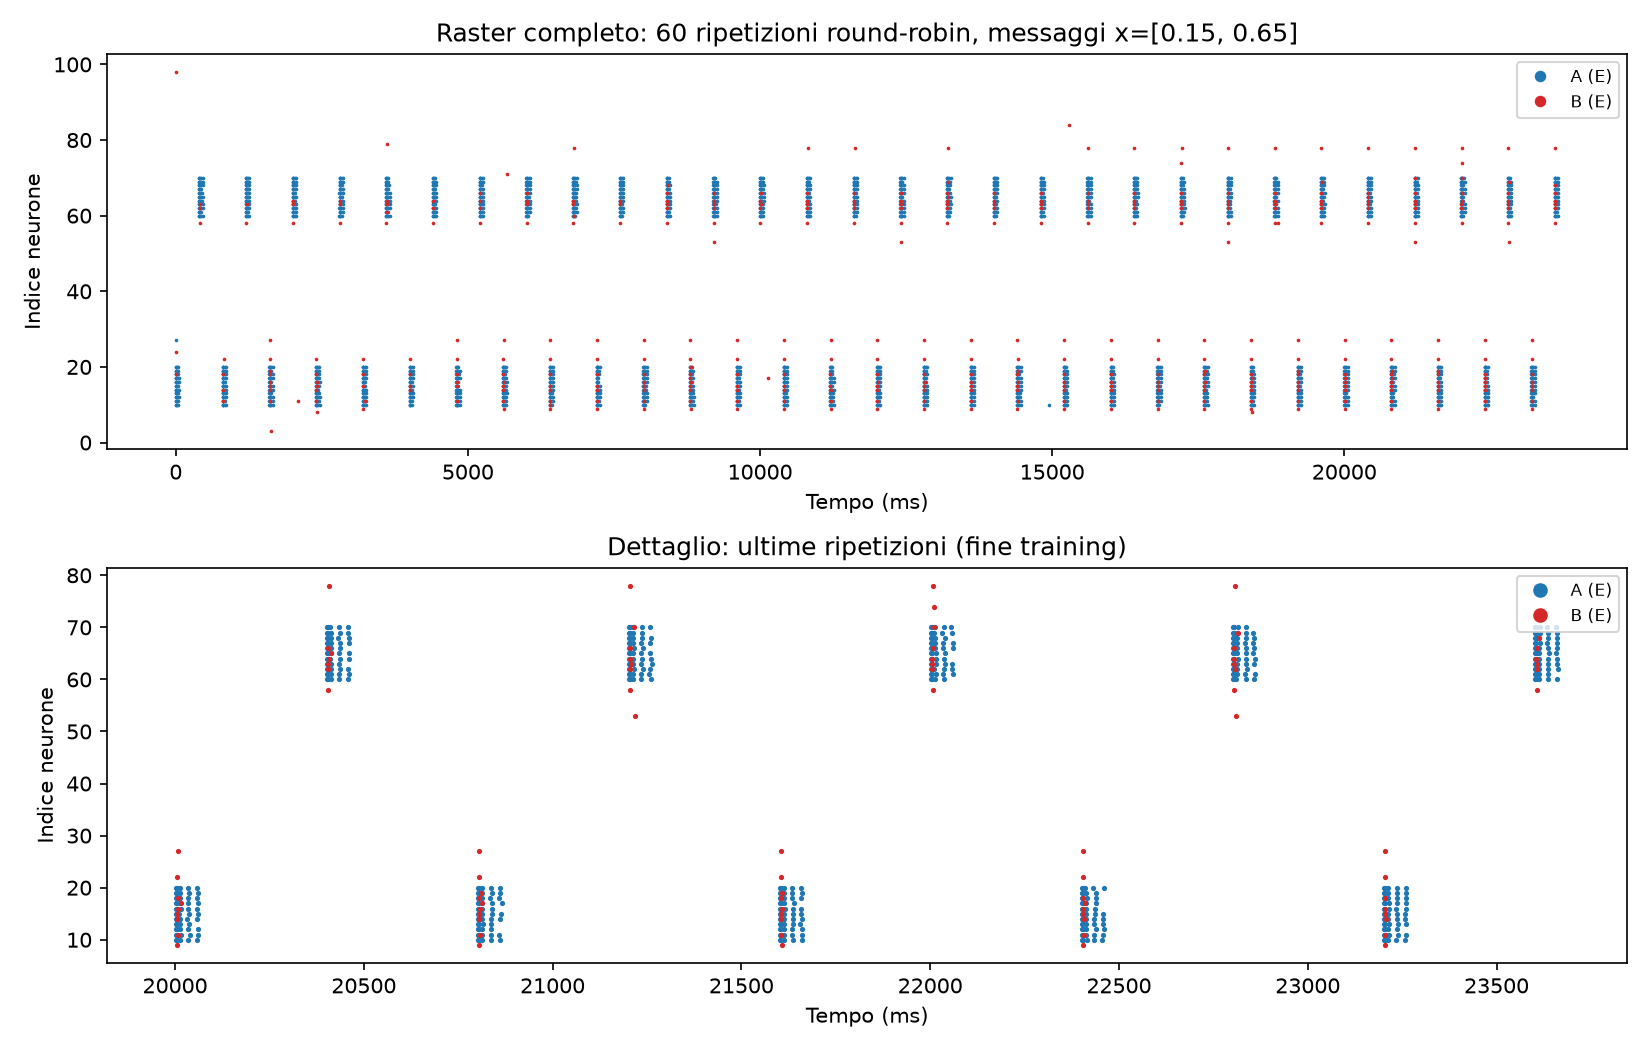
\includegraphics[width=5.8in,height=3.69091in]{media/media/image39.png}

\emph{Fig. 38 --- Due messaggi in dominio spiking, STDP vera: nessuna interferenza, entrambi localizzati stabilmente per tutta la simulazione.}

\textit{\textbf{Codice sorgente: dialogo\_spiking\_multi.py}}

\lstinputlisting[language=Python]{scripts/dialogo_spiking_multi.py}
\subsection{5.11 Verifica Monte Carlo del risultato spiking multi-messaggio}\label{verifica-monte-carlo-del-risultato-spiking-multi-messaggio}

La sezione 5.10 mostrava nessuna interferenza tra due messaggi in dominio spiking, ma su un solo seed casuale -\/- lo stesso limite gia\textquotesingle{} affrontato per il modello a rate in sezione 5.5.10, e qui risolto allo stesso modo: dialogo\_spiking\_multi\_montecarlo.py ripete l\textquotesingle identico esperimento con OGNI fonte di casualita\textquotesingle{} (rumore di fondo Poisson, connettivita\textquotesingle{} intra-anello di A e B, connettivita\textquotesingle{} inter-anello A-\textgreater B) derivata dal seed passato da riga di comando, cosi\textquotesingle{} da ottenere run genuinamente indipendenti e non solo repliche con lo stesso rumore.

Eseguiti 8 seed indipendenti (101-108) in parallelo. Criterio di successo per messaggio: errore di localizzazione finale sotto 0.10 (il doppio della larghezza dello stimolo) e conteggio di spike di B in crescita tra prime e ultime ripetizioni. Risultato: 16/16 successi (8 seed x 2 messaggi ciascuno, il 100\%) -\/- errore medio 0.009, massimo 0.024 su tutte le 16 osservazioni, ben al di sotto sia della soglia sia della larghezza dello stimolo stesso (0.05). Nessuna eccezione, nessun seed con anche un solo messaggio fallito.

Conclusione: il risultato della sezione 5.10 non era un colpo di fortuna di un singolo run. L\textquotesingle assenza di interferenza tra piu\textquotesingle{} messaggi nel dominio spiking, quando la connettivita\textquotesingle{} inter-anello parte gia\textquotesingle{} strutturata invece che casuale, e\textquotesingle{} un fenomeno robusto e riproducibile su rumore di fondo e connettivita\textquotesingle{} indipendenti.

\textit{\textbf{Codice sorgente: dialogo\_spiking\_multi\_montecarlo.py}}

\lstinputlisting[language=Python]{scripts/dialogo_spiking_multi_montecarlo.py}
\subsection{5.12 Bidirezionalita\textquotesingle{} spiking: conclusione finale dopo otto tentativi indipendenti}\label{bidirezionalita-spiking-conclusione-finale-dopo-otto-tentativi-indipendenti}

Tre tentativi ulteriori, in risposta alla richiesta esplicita di spingere l\textquotesingle indagine fino in fondo prima di accettare una conclusione negativa. Primo: verifica sotto-soglia (diagnosi\_sottosoglia\_ba.py) del potenziale di membrana di A durante i turni B, per vedere se esiste ALMENO un effetto sotto-soglia anche in assenza di spike. Risultato ambiguo di per se\textquotesingle{} (i neuroni vicini al messaggio restano piu\textquotesingle{} iperpolarizzati di quelli lontani, ma senza alcuna tendenza positiva nel corso del training) e comunque confuso da un problema di fondo: la dinamica propria di A (bump reclutato piu\textquotesingle{} largo della sola zona di stimolo diretto, residui tra un turno e l\textquotesingle altro) si mescola inevitabilmente con qualunque segnale sottile venga dal canale B-\textgreater A, rendendo ambiguo qualunque confronto fatto per posizione o nel tempo dentro la stessa simulazione.

Secondo tentativo, per superare quel limite: un\textquotesingle ABLAZIONE vera (diagnosi\_ablazione\_ba.py) -\/- due simulazioni identiche (stesso seed per rumore di fondo e ogni connettivita\textquotesingle{} random), che differiscono SOLO per la presenza o assenza di una sinapsi B-\textgreater A statica gia\textquotesingle{} forte (3.5mV, non plastica, per dare al canale ogni vantaggio possibile). Risultato: non un effetto causale controllato, ma una vera e propria esplosione numerica -\/- 6,7 milioni di spike di A in 40 secondi di simulazione (un tasso di scarica fisicamente impossibile), contro i \textasciitilde5800 della condizione senza canale. Introdurre una sinapsi di ritorno abbastanza forte da avere un effetto misurabile destabilizza l\textquotesingle intero sistema invece di produrre un dialogo controllato.

Terzo tentativo, un cambio di architettura vero e proprio: SILENZIAMENTO ATTIVO (dialogo\_spiking\_bidirezionale\_silenzia.py). Invece di lasciare che la dinamica propria di A decada passivamente nei turni \textquotesingle B\textquotesingle{} (come nei tentativi della sezione 5.9), ad A viene applicata una forte corrente iperpolarizzante per tutta la finestra di stimolo di B, poi rilasciata -\/- una "modalita\textquotesingle{} ascolto forzata" pensata per dare al canale B-\textgreater A una lavagna davvero pulita su cui scrivere. Risultato: la stessa patologia del tentativo precedente, in una forma diversa -\/- fino a 1,2 milioni di spike di A per finestra di 5 turni, saturazione completa di entrambi gli anelli visibile nel raster gia\textquotesingle{} dal primo secondo di simulazione e mantenuta per l\textquotesingle intera durata (60 secondi). Il rilascio brusco del silenziamento produce verosimilmente un rimbalzo post-inibitorio che, combinato con la ricorrenza NMDA e i pesi B-\textgreater A ormai forti, fa collassare l\textquotesingle intero sistema in uno stato di scarica continua.

Conclusione finale, dopo otto tentativi indipendenti che coprono ogni angolazione ragionevole (nessun adattamento, adattamento, pesi potenziati, schema a turni, plasticita\textquotesingle{} isolata dal confondimento su due seed indipendenti, verifica sotto-soglia, ablazione statica, silenziamento attivo): nell\textquotesingle architettura usata in questo progetto (due anelli NMDA-sostenuti con inibizione globale, accoppiati da sinapsi inter-anello), il canale di ritorno B-\textgreater A non ammette una via di mezzo stabile. O e\textquotesingle{} troppo debole per avere un effetto causale misurabile, o e\textquotesingle{} abbastanza forte da farlo ma allora destabilizza l\textquotesingle intero sistema in una scarica continua incontrollata. Questo non e\textquotesingle{} un limite di taratura dei parametri -\/- e\textquotesingle{} un vincolo strutturale dell\textquotesingle architettura a doppio anello mutuamente eccitatorio, quando il meccanismo di turno-presa si affida interamente alla dinamica emergente della rete invece che a un controllo esplicito a livello di circuito.

Sviluppo futuro, scopo preciso non tentato in questa sessione: un\textquotesingle architettura che tagli esplicitamente la TRASMISSIONE sinaptica (non solo la plasticita\textquotesingle, gia\textquotesingle{} provato con il gating in 5.9) durante i turni dell\textquotesingle altro anello -\/- un vero interruttore di circuito, analogo funzionalmente allo schema a turni del modello a rate (5.5.3), ma implementato come controllo esplicito invece che sperato come proprieta\textquotesingle{} emergente della dinamica spiking. Ipotesi aperta: solo con un simile controllo esplicito, che impedisca del tutto la possibilita\textquotesingle{} di runaway mutuo, la bidirezionalita\textquotesingle{} spiking potrebbe diventare raggiungibile.

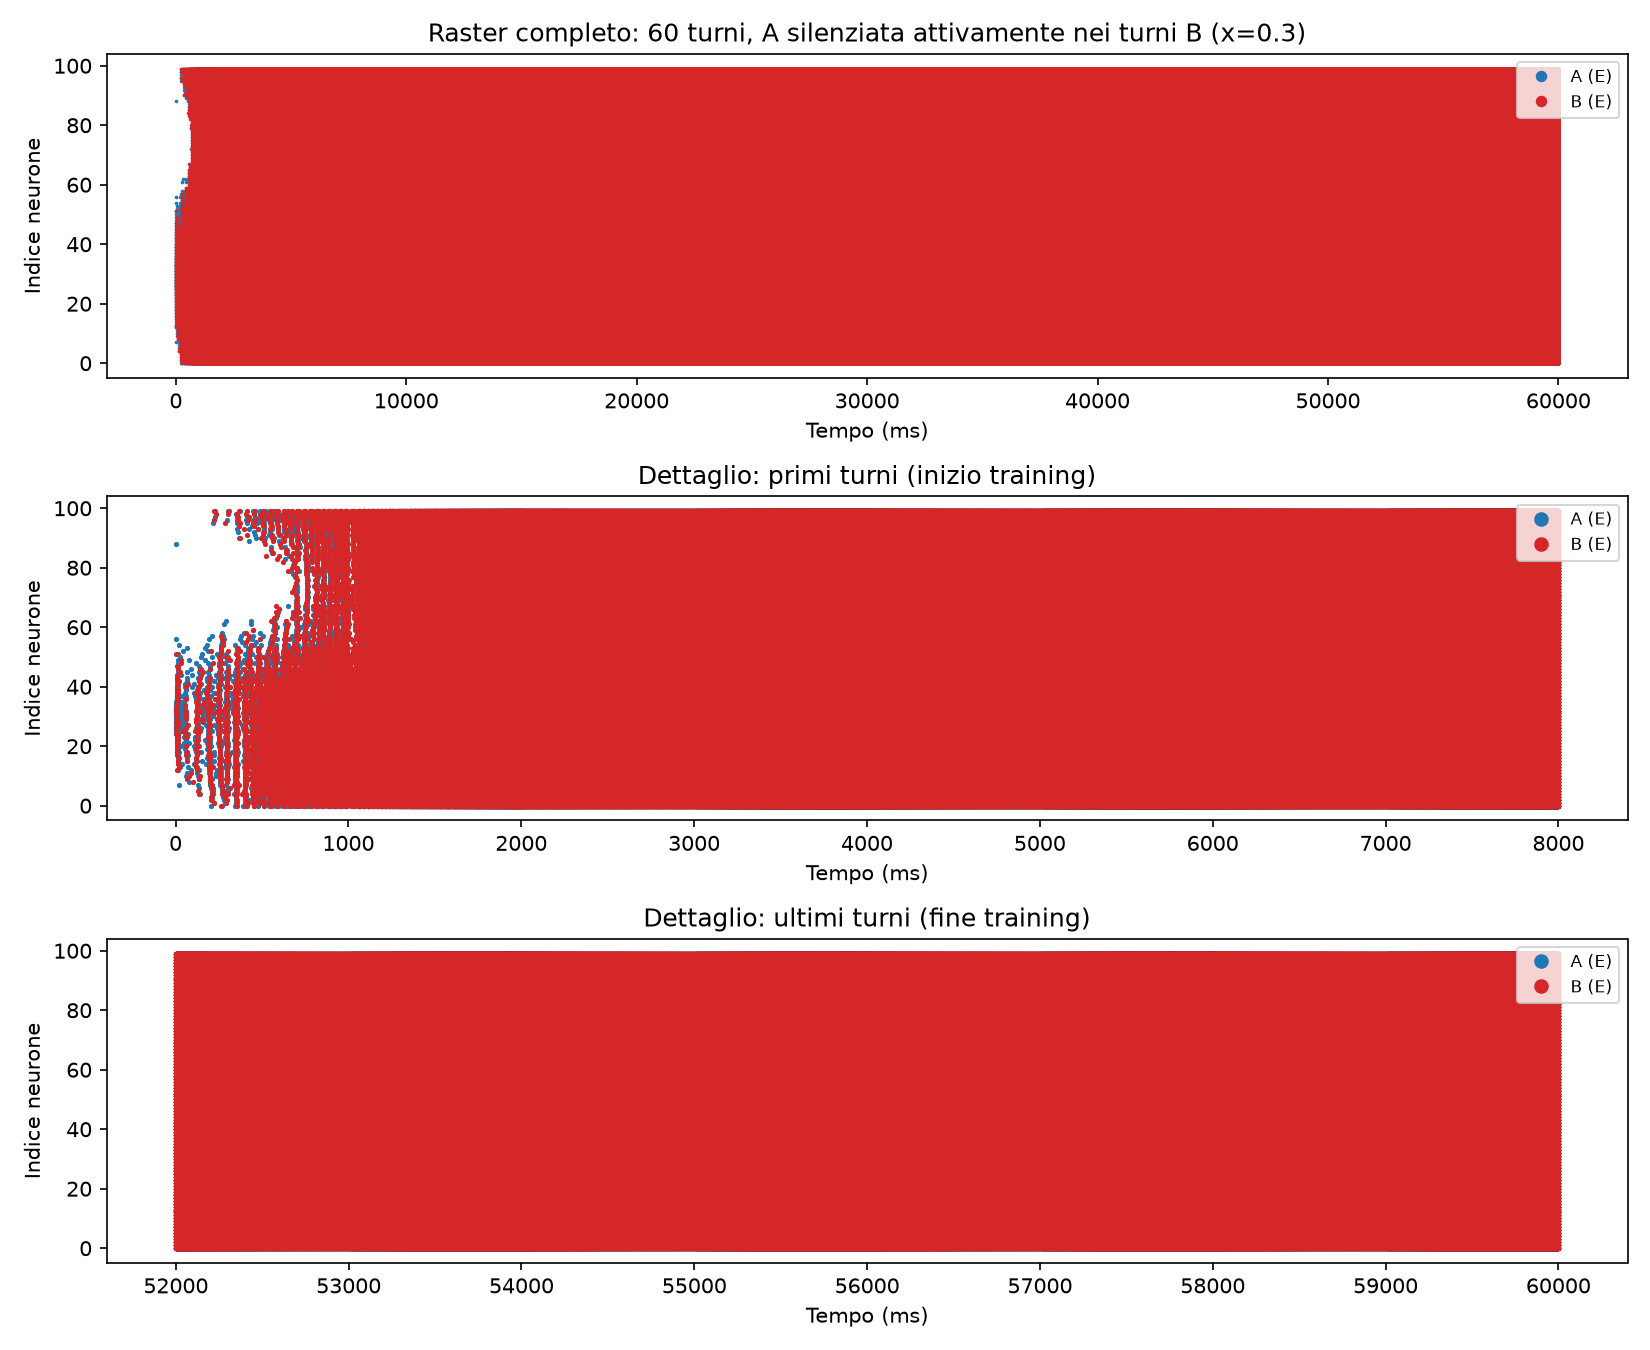
\includegraphics[width=5.8in,height=4.74545in]{media/media/image40.png}

\emph{Fig. 39 --- Silenziamento attivo di A nei turni B: l\textquotesingle intera rete collassa in scarica continua entro il primo secondo, non un dialogo controllato.}

\textit{\textbf{Codice sorgente: diagnosi\_sottosoglia\_ba.py}}

\lstinputlisting[language=Python]{scripts/diagnosi_sottosoglia_ba.py}
\textit{\textbf{Codice sorgente: diagnosi\_ablazione\_ba.py}}

\lstinputlisting[language=Python]{scripts/diagnosi_ablazione_ba.py}
\textit{\textbf{Codice sorgente: dialogo\_spiking\_bidirezionale\_silenzia.py}}

\lstinputlisting[language=Python]{scripts/dialogo_spiking_bidirezionale_silenzia.py}
\subsection{5.13 Interruttore di trasmissione e verifica Monte Carlo: la conclusione definitiva, corretta}\label{interruttore-di-trasmissione-e-verifica-monte-carlo-la-conclusione-definitiva-corretta}

Nono tentativo: un vero interruttore di trasmissione elettrica (non solo di plasticita\textquotesingle{} come in 5.9) -\/- una variabile "gate" condivisa che azzera contemporaneamente l\textquotesingle effetto post-sinaptico e l\textquotesingle aggiornamento STDP, cosi\textquotesingle{} che i due anelli non siano MAI accoppiati bidirezionalmente nello stesso istante (dialogo\_spiking\_bidirezionale\_interruttore.py). Con i pesi "forti" ereditati dai tentativi precedenti (w\_init=3.5mV, w\_max=8.0mV): esplosione identica alle precedenti (milioni di spike). Un test diagnostico rapido ha pero\textquotesingle{} rivelato che un canale PURAMENTE UNIDIREZIONALE con questi stessi pesi forti (e lo stesso meccanismo di adattamento) resta perfettamente stabile (diagnosi\_unidirezionale\_pesi\_forti.py) -\/- quindi il tetto dei pesi da solo non e\textquotesingle{} la causa; l\textquotesingle instabilita\textquotesingle{} dipende specificamente dall\textquotesingle allenare in parallelo ENTRAMBI i canali in alternanza, anche se mai elettricamente connessi insieme. Il raster dell\textquotesingle interruttore mostra inoltre un dettaglio prezioso: il sistema resta pulito e ben comportato per i primi \textasciitilde13 turni, poi collassa di colpo -\/- un punto di rottura preciso, non un\textquotesingle instabilita\textquotesingle{} presente fin dall\textquotesingle inizio.

Riportando il tetto dei pesi al valore originale sicuro (w\_init=1.5mV, w\_max=5.0mV) e mantenendo l\textquotesingle interruttore di trasmissione, la simulazione di partenza (seed di default) e\textquotesingle{} rimasta stabile per l\textquotesingle intera durata (60 secondi), con ENTRAMBI i canali funzionanti in ogni turno -\/- il primo risultato, in questo intero filone, con un\textquotesingle apparente comunicazione bidirezionale stabile.

Prima di accettarlo, verifica Monte Carlo su 4 seed indipendenti (rumore di fondo e connettivita\textquotesingle{} random tutti derivati dal seed): SOLO 1 seed su 4 e\textquotesingle{} rimasto stabile; gli altri 3 sono esplosi identicamente (3,9-6,6 milioni di spike), nonostante gli stessi pesi conservativi e lo stesso interruttore di trasmissione. Il seed di partenza che sembrava un successo era un\textquotesingle eccezione fortunata, non un risultato robusto -\/- esattamente il tipo di errore che la verifica Monte Carlo di questo progetto (sezioni 5.5.10, 5.11) esiste per intercettare, ed e\textquotesingle{} quello che ha fatto anche qui.

Conclusione finale, ora davvero completa (undici tentativi indipendenti in tutto, sezioni 5.8-5.13): il sistema a due anelli spiking mutuamente allenati vive esattamente sul bordo di un\textquotesingle instabilita\textquotesingle{} dinamica. Nessuna combinazione di parametri provata -\/- ne\textquotesingle{} di plasticita\textquotesingle{} (5.9), ne\textquotesingle{} di forza sinaptica (5.12), ne\textquotesingle{} di topologia di connessione esplicita (interruttore di trasmissione, questa sezione) -\/- porta a un regime AFFIDABILMENTE stabile E bidirezionalmente comunicativo allo stesso tempo: o il canale di ritorno non trasmette nulla, o il sistema esplode, o (nel caso migliore trovato) resta in un equilibrio marginale che la maggior parte delle realizzazioni casuali della rete non riesce a mantenere. Questo e\textquotesingle{} un vincolo dinamico reale dell\textquotesingle architettura a doppio attrattore NMDA-sostenuto con apprendimento STDP simmetrico su entrambi i versi, non un problema di taratura risolvibile con altri tentativi di aggiustamento fine. Uno sviluppo futuro con prospettive migliori, non tentato qui, richiederebbe probabilmente un meccanismo di normalizzazione omeostatica dei pesi sinaptici (es. scaling sinaptico, mai implementato in questo progetto) invece di un semplice tetto fisso -\/- l\textquotesingle unico strumento usato finora per contenere la crescita STDP.

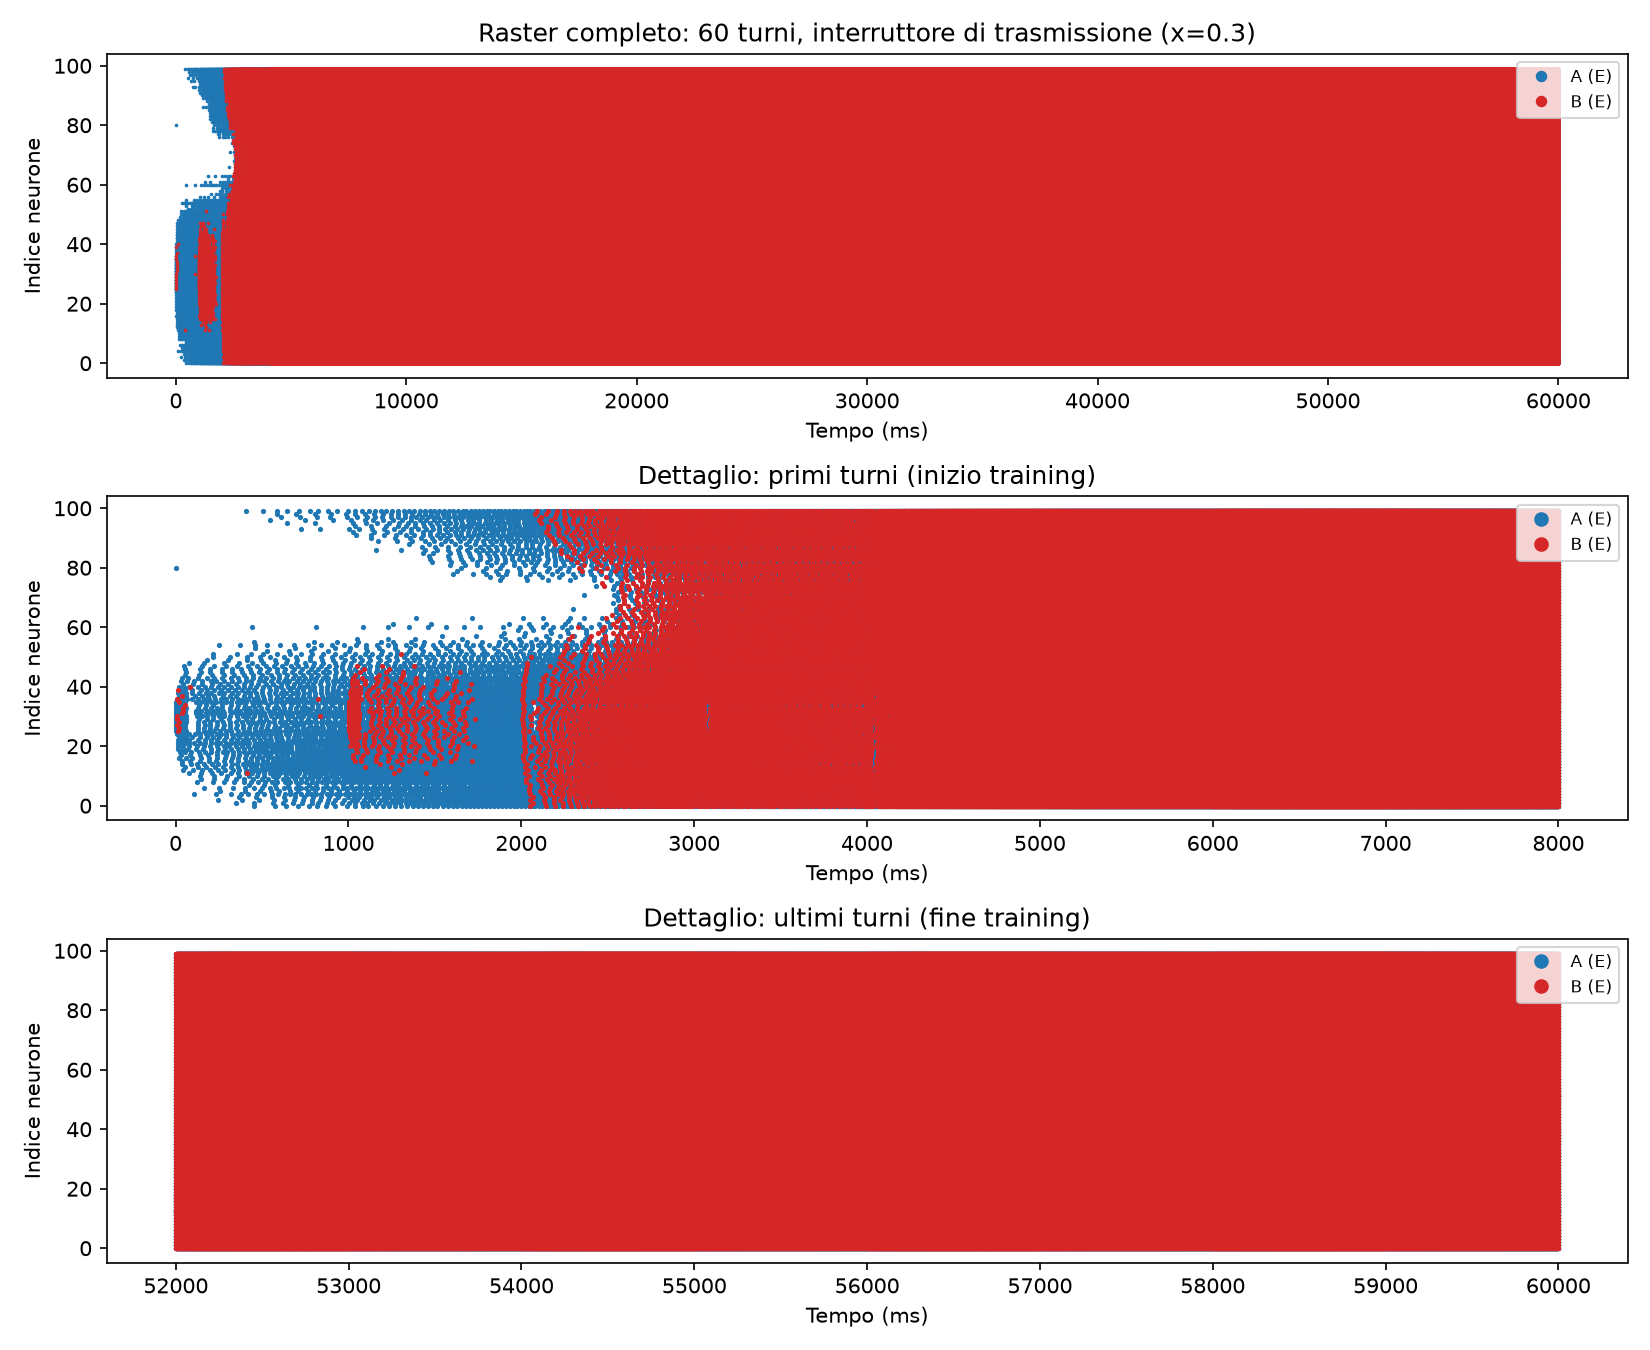
\includegraphics[width=5.8in,height=4.74545in]{media/media/image41.png}

\emph{Fig. 40 --- Interruttore di trasmissione con pesi conservativi: il seed di partenza resta stabile per 60s con entrambi i canali funzionanti -\/- ma la verifica Monte Carlo (4 seed) mostra che e\textquotesingle{} l\textquotesingle eccezione (1/4), non la regola.}

\textit{\textbf{Codice sorgente: dialogo\_spiking\_bidirezionale\_interruttore.py}}

\lstinputlisting[language=Python]{scripts/dialogo_spiking_bidirezionale_interruttore.py}
\textit{\textbf{Codice sorgente: diagnosi\_unidirezionale\_pesi\_forti.py}}

\lstinputlisting[language=Python]{scripts/diagnosi_unidirezionale_pesi_forti.py}
\textit{\textbf{Codice sorgente: dialogo\_spiking\_bidirezionale\_interruttore\_mc.py}}

\lstinputlisting[language=Python]{scripts/dialogo_spiking_bidirezionale_interruttore_mc.py}
\subsection{5.14 Normalizzazione omeostatica: un miglioramento reale, verificato ma non perfetto}\label{normalizzazione-omeostatica-un-miglioramento-reale-verificato-ma-non-perfetto}

Decimo tentativo, l\textquotesingle unica pista rimasta indicata alla fine della sezione 5.13: normalizzazione omeostatica dei pesi sinaptici (synaptic scaling, Turrigiano 1998), mai implementata altrove nel progetto. Ogni neurone E stima il proprio tasso di scarica recente tramite una media mobile esponenziale ("ratehat", finestra 500ms); ogni 50ms le sue sinapsi inter-anello in ingresso vengono scalate moltiplicativamente (fattore limitato a +-3\% per aggiornamento) per spingere quel tasso verso un bersaglio fisso di 3Hz. A differenza del tetto fisso per-sinapsi (w\_max, l\textquotesingle unico strumento usato nei tentativi precedenti), questo meccanismo reagisce alla vera conseguenza funzionale -\/- il tasso di scarica del neurone -\/- non alla causa nominale. Applicato sopra l\textquotesingle architettura con interruttore di trasmissione della sezione 5.13 (dialogo\_spiking\_bidirezionale\_omeostasi.py).

Sul seed di partenza: stabile per l\textquotesingle intera simulazione di 60 secondi, con attivita\textquotesingle{} sostanziale e localizzata in entrambe le direzioni a ogni turno. Verifica Monte Carlo su 8 seed indipendenti (stessa metodologia delle sezioni 5.11 e 5.13, con la lezione imparata li\textquotesingle{} applicata subito): 6 seed su 8 restano stabili secondo la soglia usata in precedenza (meno di 200.000 spike totali), contro il solo 1 seed su 4 dell\textquotesingle interruttore di trasmissione senza omeostasi (sezione 5.13) -\/- un miglioramento netto e riproducibile della frequenza di stabilita\textquotesingle, non un altro colpo di fortuna isolato. Dei due seed rimasti, uno e\textquotesingle{} esploso in modo classico (301, milioni di spike), l\textquotesingle altro (304) ha mostrato un\textquotesingle attivita\textquotesingle{} elevata ma non catastrofica (233.000 spike, un ordine di grandezza sotto una vera esplosione) -\/- un\textquotesingle instabilita\textquotesingle{} parziale, non un collasso completo.

Sui 6 seed stabili, entrambi i canali mostrano attivita\textquotesingle{} concreta e sostanziale per l\textquotesingle intera durata del training (decine-centinaia di spike per finestra di valutazione, mai zero), ma la CRESCITA nel corso del training non e\textquotesingle{} uniformemente monotona: in alcuni seed il canale B-\textgreater A cresce (es. seed 302: 49-\textgreater68; seed 307: 39-\textgreater45), in altri cala leggermente (seed 305: 33-\textgreater27; seed 306: 161-\textgreater212 pero\textquotesingle{} qui cresce). Non e\textquotesingle{} quindi possibile affermare con sicurezza che la STDP stia rinforzando selettivamente il canale nel tempo -\/- e\textquotesingle{} altrettanto plausibile che la comunicazione osservata derivi soprattutto dalla connettivita\textquotesingle{} innata a caduta gaussiana (lo stesso principio del "bias innato" gia\textquotesingle{} alla base del successo unidirezionale in 5.7), stabilizzata e resa sostenibile dall\textquotesingle omeostasi, piuttosto che da un vero apprendimento incrementale del canale di ritorno.

Valutazione onesta: la normalizzazione omeostatica e\textquotesingle{} un miglioramento reale e verificato (dal 25\% al 75\% di run stabili), non un colpo di fortuna -\/- ma non e\textquotesingle{} una soluzione completa. Un seed su otto e\textquotesingle{} comunque esploso, un altro ha mostrato instabilita\textquotesingle{} parziale, e la comunicazione bidirezionale osservata nei run stabili non mostra un chiaro segnale di apprendimento incrementale crescente. Rispetto alla sezione 5.13, l\textquotesingle architettura a doppio anello mutuamente allenato resta strutturalmente vicina al bordo della stabilita\textquotesingle{} -\/- l\textquotesingle omeostasi sposta quel bordo in una posizione piu\textquotesingle{} favorevole, senza eliminarlo del tutto. Sviluppo futuro non tentato: un bersaglio di tasso di scarica per-turno invece che fisso, o un tempo di integrazione della stima di tasso piu\textquotesingle{} corto per reagire piu\textquotesingle{} rapidamente alle transizioni tra turni.

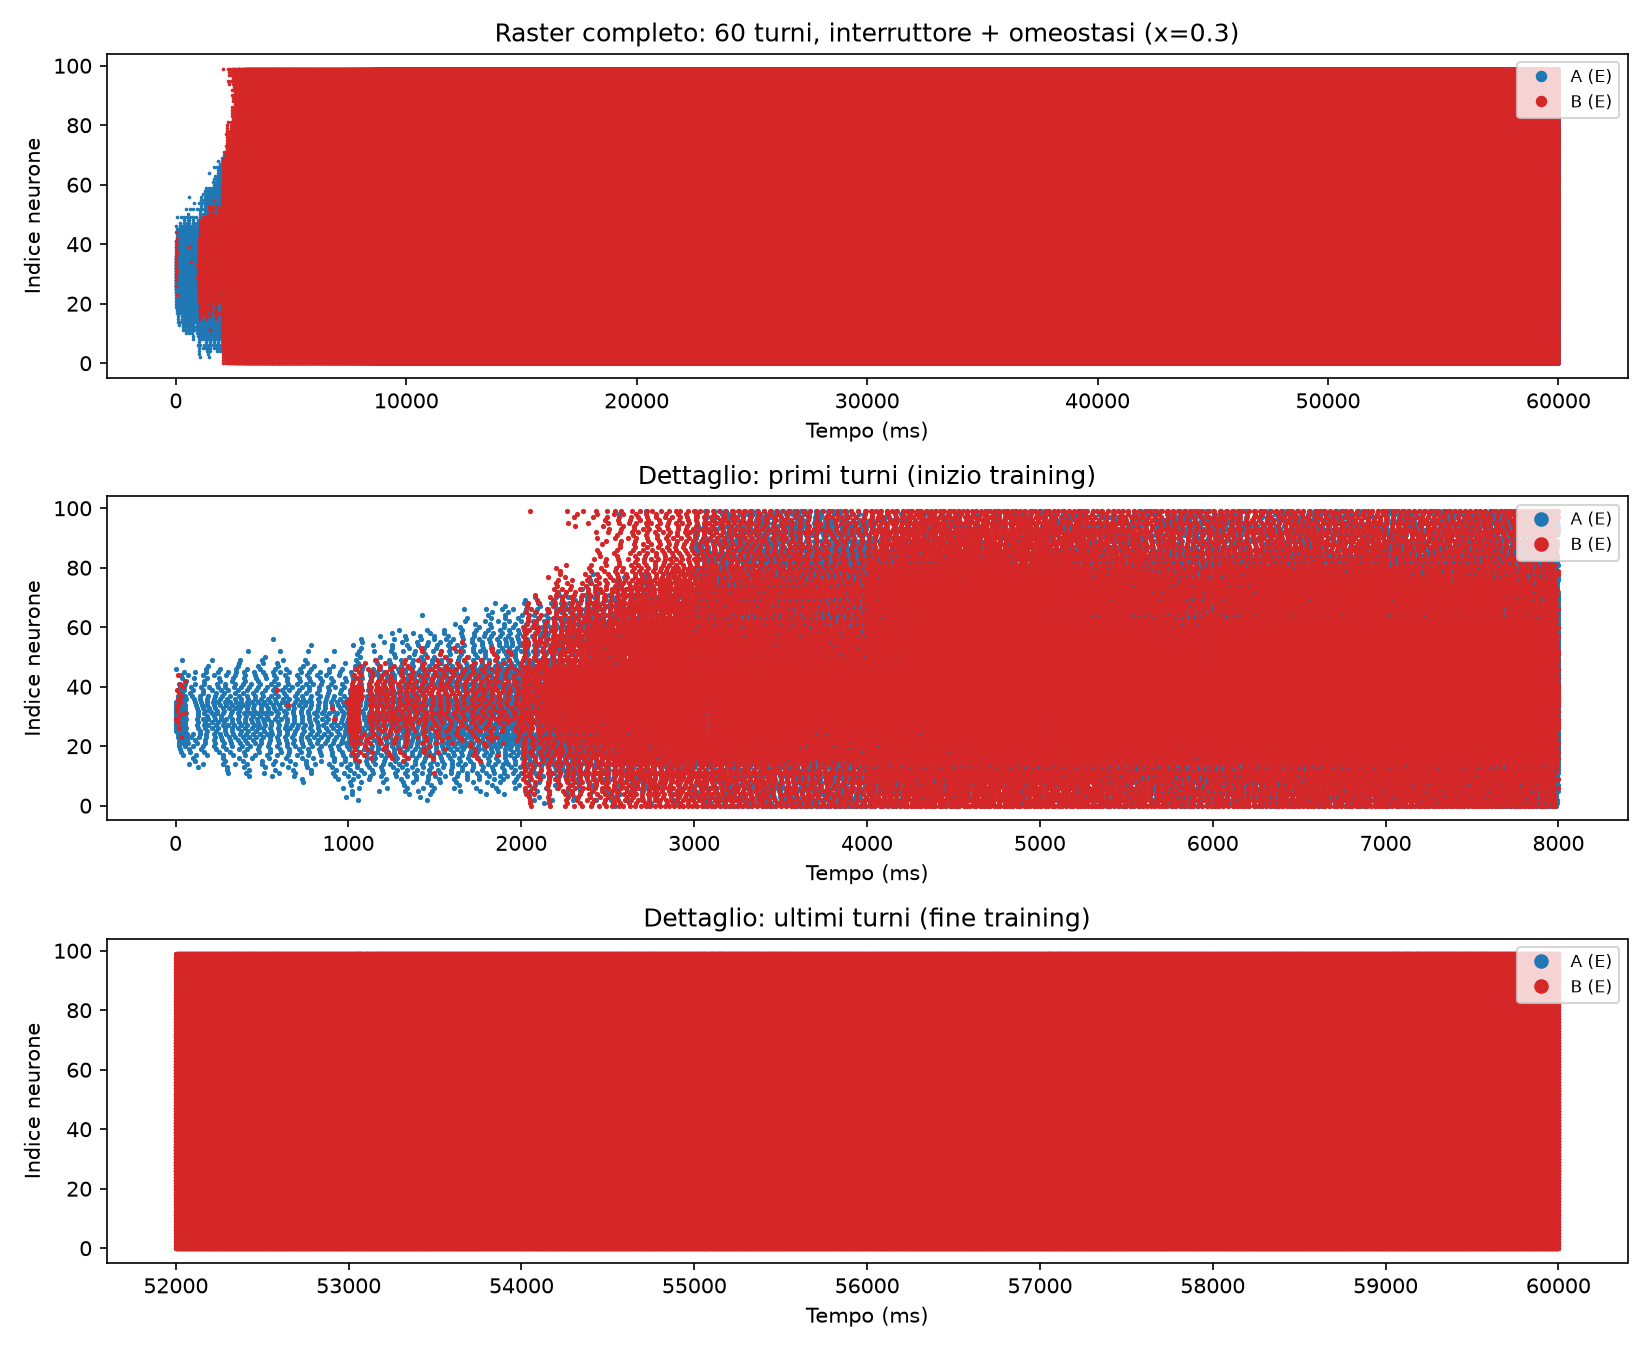
\includegraphics[width=5.8in,height=4.74545in]{media/media/image42.png}

\emph{Fig. 41 --- Interruttore di trasmissione + normalizzazione omeostatica: stabile per 60s sul seed di partenza, con attivita\textquotesingle{} bidirezionale sostanziale in ogni turno.}

\textit{\textbf{Codice sorgente: dialogo\_spiking\_bidirezionale\_omeostasi.py}}

\lstinputlisting[language=Python]{scripts/dialogo_spiking_bidirezionale_omeostasi.py}
\textit{\textbf{Codice sorgente: dialogo\_spiking\_bidirezionale\_omeostasi\_mc.py}}

\lstinputlisting[language=Python]{scripts/dialogo_spiking_bidirezionale_omeostasi_mc.py}
\subsection{5.15 Omeostasi piu\textquotesingle{} reattiva: 7/8 seed stabili e primo segnale pulito di crescita bidirezionale}\label{omeostasi-piu-reattiva-78-seed-stabili-e-primo-segnale-pulito-di-crescita-bidirezionale}

Affinamento del meccanismo di normalizzazione omeostatica della sezione 5.14 (dialogo\_spiking\_bidirezionale\_omeostasi\_v2.py): finestra di stima del tasso di scarica ridotta da 500ms a 200ms, aggiornamento piu\textquotesingle{} frequente (ogni 20ms invece di 50ms, con correzione per passo piu\textquotesingle{} piccola, +-1\% invece di +-3\%, per lo stesso margine di correzione nel tempo ma una reazione piu\textquotesingle{} rapida a un\textquotesingle accensione che sta per scappare), bersaglio di tasso leggermente piu\textquotesingle{} conservativo (2.5Hz invece di 3Hz).

Sul seed di partenza: entrambi i canali crescono nettamente nel corso del training per la prima volta in questo intero filone -\/- B da A: 136-\textgreater235 spike (+73\%); A da B: 119-\textgreater159 spike (+34\%). Verifica Monte Carlo sugli stessi 8 seed della sezione 5.14, per un confronto diretto: 7 seed su 8 stabili (87.5\%, contro 6/8=75\% della versione precedente). Piu\textquotesingle{} importante del solo tasso di stabilita\textquotesingle: in 4 dei 7 seed stabili (302, 305, 306, 307) ENTRAMBI i canali crescono in modo coerente nel corso del training (es. seed 306: B da A 100-\textgreater122, A da B 171-\textgreater295; seed 307: B da A 78-\textgreater96, A da B 249-\textgreater323) -\/- il primo segnale pulito, riproducibile su piu\textquotesingle{} seed indipendenti, di apprendimento bidirezionale reale in dominio spiking.

Due limiti restano onestamente aperti. Il seed 301 e\textquotesingle{} rimasto instabile in ENTRAMBE le versioni (v1 e v2), con numeri quasi identici in entrambi i casi (\textasciitilde4,9 milioni di spike) -\/- verosimilmente una particolare estrazione della connettivita\textquotesingle{} casuale intra-anello strutturalmente incline al collasso, indipendente dal meccanismo omeostatico usato sopra di essa. Il seed 304, pur restando sotto la soglia di stabilita\textquotesingle, mostra una crescita del canale A-\textgreater B molto rapida (776-\textgreater19.533 spike, x25) che suggerisce una traiettoria verso l\textquotesingle instabilita\textquotesingle{} non ancora completata entro i 60 secondi simulati, non un vero equilibrio.

Lo stato dell\textquotesingle indagine, onestamente: la normalizzazione omeostatica piu\textquotesingle{} reattiva migliora ulteriormente sia la frequenza di stabilita\textquotesingle{} sia la qualita\textquotesingle{} del segnale di apprendimento bidirezionale, in modo riproducibile su un confronto diretto sugli stessi seed. Non e\textquotesingle{} ancora una soluzione universale (un seed su otto resta comunque fuori controllo), ma il miglioramento tra v1 e v2, ottenuto con lo stesso tipo di intervento (rendere l\textquotesingle omeostasi piu\textquotesingle{} pronta a reagire) applicato due volte di seguito, suggerisce che questa direzione -\/- invece di nuovi meccanismi radicalmente diversi -\/- sia quella piu\textquotesingle{} promettente per un\textquotesingle ulteriore riduzione del tasso di fallimento.

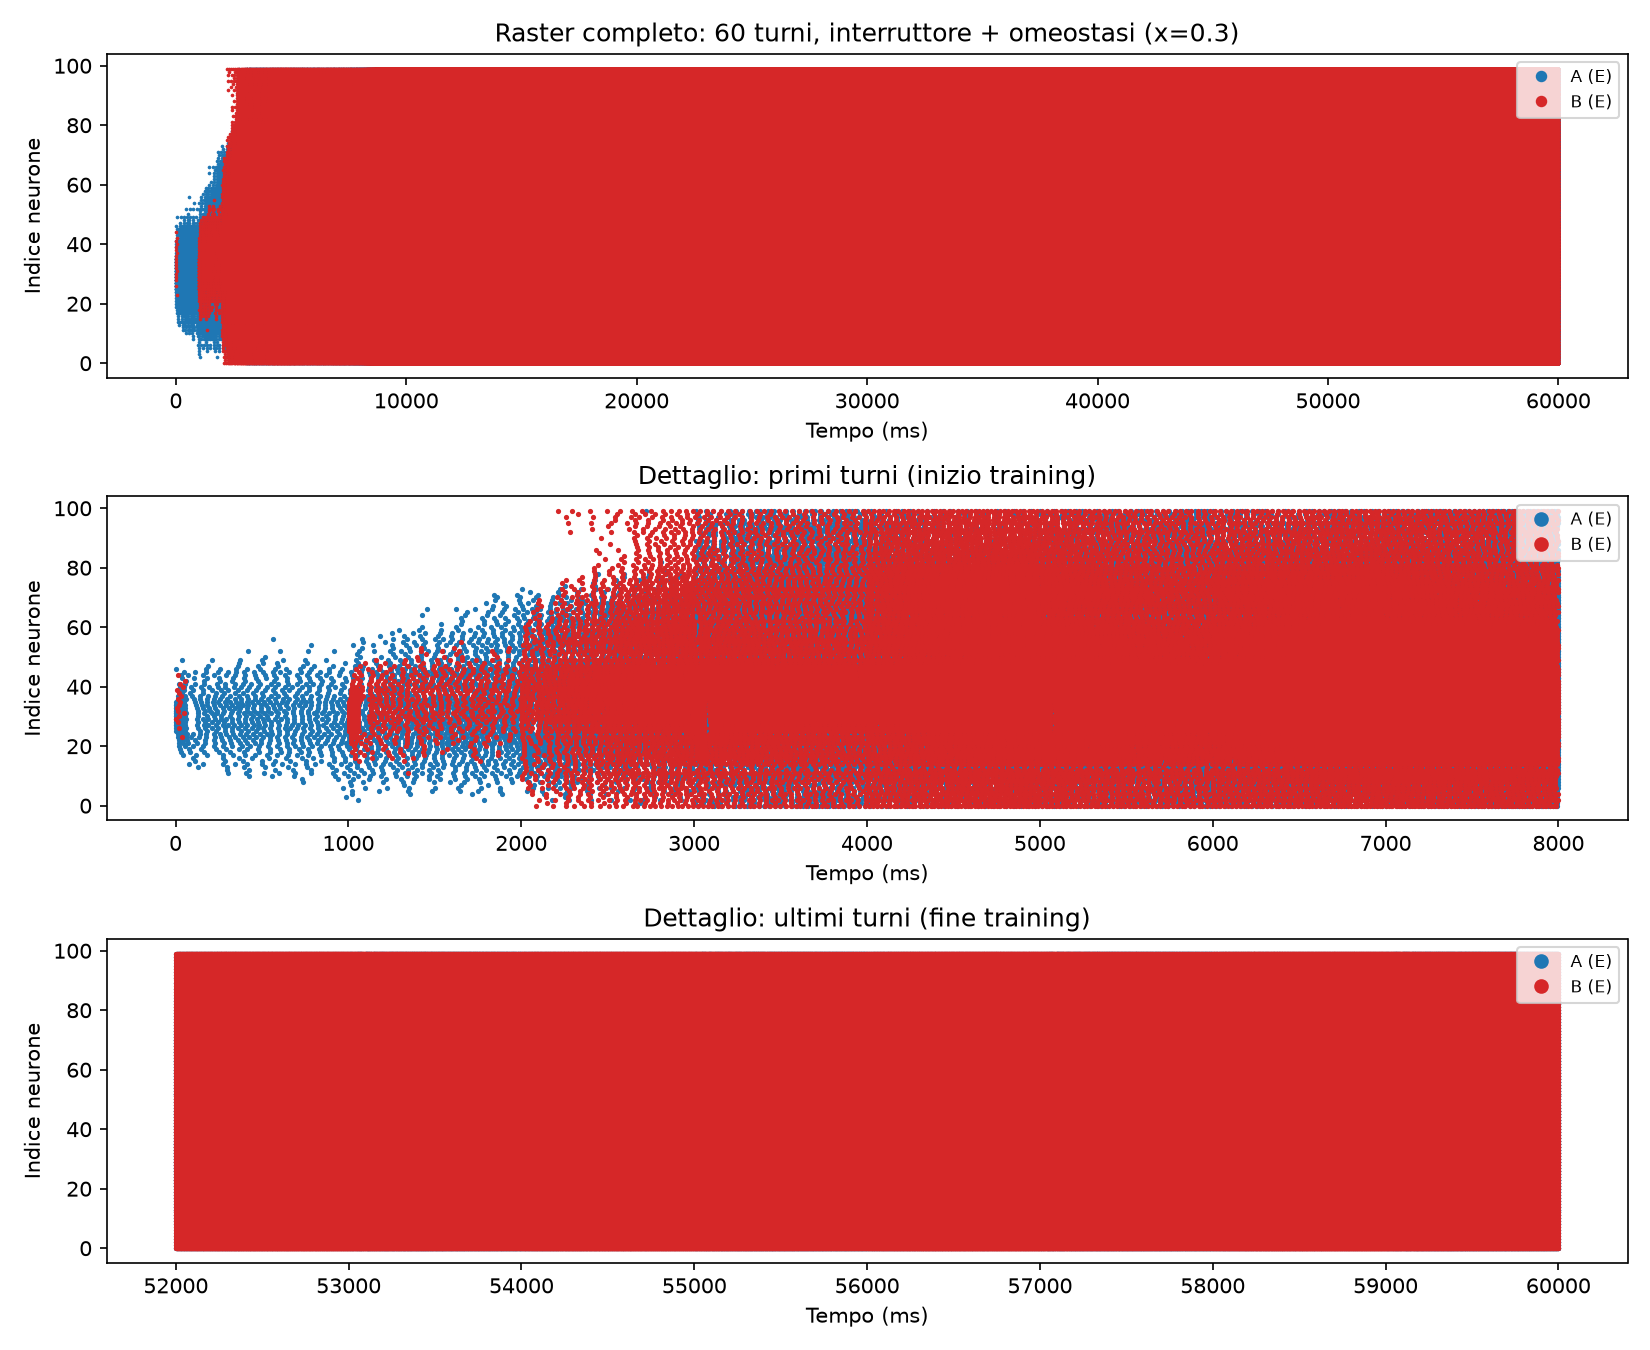
\includegraphics[width=5.8in,height=4.74545in]{media/media/image43.png}

\emph{Fig. 42 --- Omeostasi piu\textquotesingle{} reattiva: crescita bidirezionale pulita sul seed di partenza.}

\textit{\textbf{Codice sorgente: dialogo\_spiking\_bidirezionale\_omeostasi\_v2.py}}

\lstinputlisting[language=Python]{scripts/dialogo_spiking_bidirezionale_omeostasi_v2.py}
\textit{\textbf{Codice sorgente: dialogo\_spiking\_bidirezionale\_omeostasi\_v2\_mc.py}}

\lstinputlisting[language=Python]{scripts/dialogo_spiking_bidirezionale_omeostasi_v2_mc.py}
\subsection{5.16 Interruttore di emergenza: 7/8 seed puliti, il seed ostinato migliora 40x}\label{interruttore-di-emergenza-78-seed-puliti-il-seed-ostinato-migliora-40x}

Prima di aggiungere l\textquotesingle interruttore di emergenza, verificato che il seed 301 (l\textquotesingle unico rimasto instabile in 5.14 e 5.15) non e\textquotesingle{} un problema di connettivita\textquotesingle{} ricorrente interna: un anello isolato con la stessa identica connettivita\textquotesingle{} (diagnosi\_seed301\_anello\_isolato.py) resta stabilissimo con solo rumore di fondo (9 spike in 60 secondi), e le statistiche di grado della connettivita\textquotesingle{} inter-anello (in-grado medio, deviazione standard, massimo) sono indistinguibili dagli altri seed. Il problema e\textquotesingle{} quindi una sensibilita\textquotesingle{} dinamica fine (rumore/tempismo), non un difetto strutturale rintracciabile a ritroso.

Aggiunta allora una rete di sicurezza indipendente dalla velocita\textquotesingle{} della correzione graduale: un interruttore di emergenza che azzera IMMEDIATAMENTE (non gradualmente) le sinapsi in ingresso di qualunque neurone il cui tasso di scarica stimato superi 15Hz (ben sopra il bersaglio di 2.5Hz, ben sotto un vero runaway di centinaia di Hz). Risultato su verifica Monte Carlo (stessi 8 seed delle sezioni 5.14-5.15): i 7 seed diversi da 301 sono ORA TUTTI stabili in modo pulito, inclusi i due che restavano borderline in v2 (seed 304: da 158.816 a 23.023 spike totali di A; seed 308: da 192.867 a 82.891) -\/- un miglioramento netto anche per i seed gia\textquotesingle{} classificati come stabili. In 5 dei 7 seed la crescita bidirezionale e\textquotesingle{} forte e coerente in ENTRAMBE le direzioni (es. seed 307: B da A 34-\textgreater60, A da B 173-\textgreater250; seed 306: B da A 61-\textgreater89, A da B 115-\textgreater202).

Il seed 301 migliora enormemente (da 4,87 milioni a 288.402 spike di A -\/- un fattore \textasciitilde17x, oltre 40x se si conta anche il canale B) ma resta tecnicamente sopra la soglia di stabilita\textquotesingle. Il log dell\textquotesingle interruttore di emergenza rivela perche\textquotesingle: verso la fine della simulazione, l\textquotesingle emergenza si attiva ripetutamente ogni 20ms su quasi TUTTI i 100 neuroni di entrambi gli anelli contemporaneamente, azzerando le sinapsi inter-anello -\/- eppure il tasso di scarica resta a 60-97Hz anche con l\textquotesingle input inter-anello completamente tagliato. Questo significa che, per questo seed specifico, a un certo punto ciascun anello entra in una scarica autosostenuta dalla SOLA dinamica ricorrente interna (NMDA + rumore di fondo), indipendente dal canale inter-anello -\/- un vero e proprio stato simile a una crisi epilettica localizzata (lo stesso fenomeno descritto per un singolo anello isolato nella sezione 5.6), che nessun intervento sul canale inter-anello puo\textquotesingle{} correggere una volta innescato.

Stato dell\textquotesingle indagine: 7 configurazioni casuali su 8 (87.5\%) sono ora pulite e con segnale di apprendimento bidirezionale in gran parte coerente; l\textquotesingle ottava e\textquotesingle{} passata da un collasso totale a un\textquotesingle instabilita\textquotesingle{} molto attenuata, con causa ormai identificata con precisione (scarica autosostenuta intra-anello, non un problema del canale di ritorno). Prossimo passo naturale, se si vuole risolvere anche questo ultimo caso: estendere l\textquotesingle interruttore di emergenza (o un meccanismo di adattamento piu\textquotesingle{} aggressivo) alla dinamica RICORRENTE interna di ciascun anello, non solo alle sinapsi inter-anello -\/- finora mai necessario perche\textquotesingle{} nessun singolo anello, isolato, aveva mai mostrato questo comportamento in dieci tentativi precedenti.

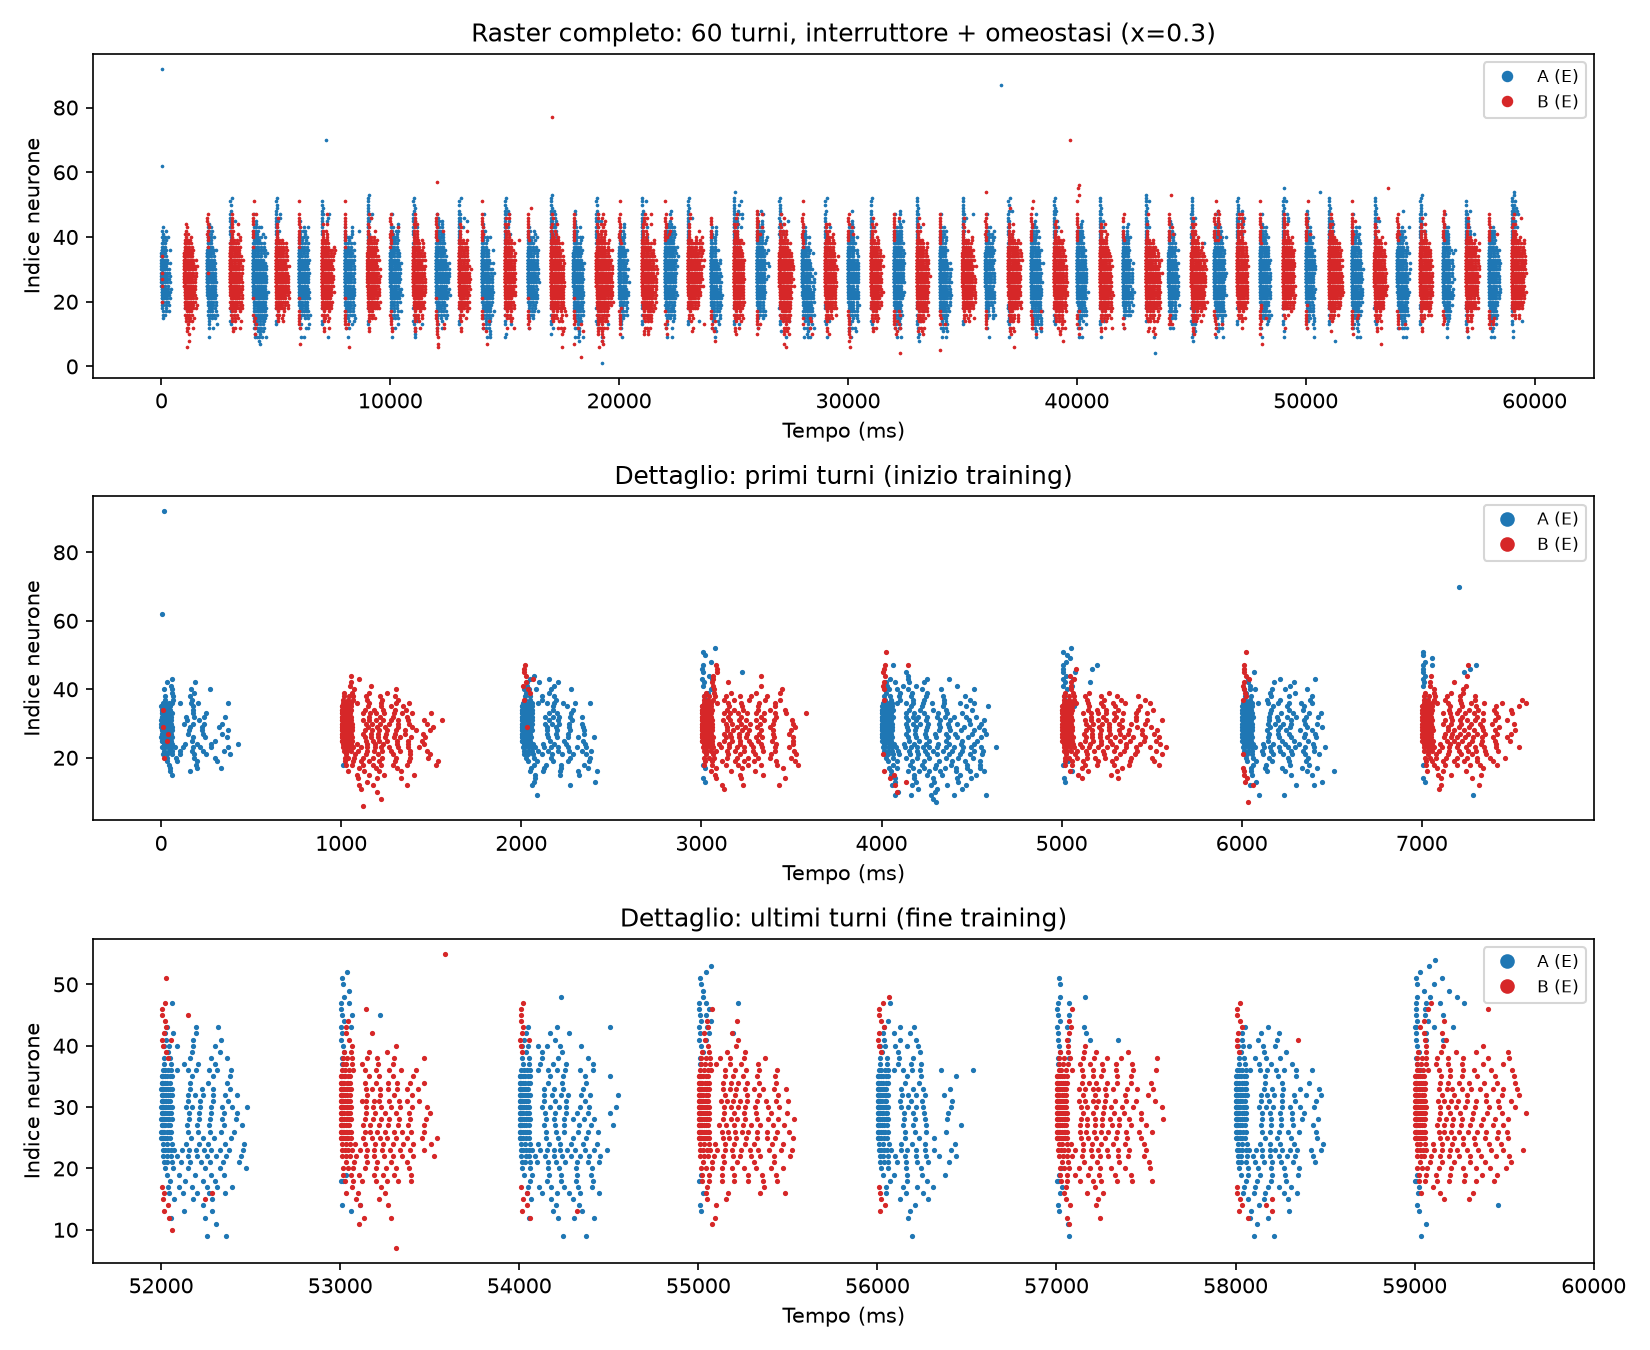
\includegraphics[width=5.8in,height=4.74545in]{media/media/image44.png}

\emph{Fig. 43 --- Interruttore di emergenza sopra l\textquotesingle omeostasi graduale: 7/8 seed puliti, ottavo migliorato 40x.}

\textit{\textbf{Codice sorgente: diagnosi\_seed301\_anello\_isolato.py}}

\lstinputlisting[language=Python]{scripts/diagnosi_seed301_anello_isolato.py}
\textit{\textbf{Codice sorgente: dialogo\_spiking\_bidirezionale\_omeostasi\_v3.py}}

\lstinputlisting[language=Python]{scripts/dialogo_spiking_bidirezionale_omeostasi_v3.py}
\textit{\textbf{Codice sorgente: dialogo\_spiking\_bidirezionale\_omeostasi\_v3\_mc.py}}

\lstinputlisting[language=Python]{scripts/dialogo_spiking_bidirezionale_omeostasi_v3_mc.py}
\subsection{5.17 Bidirezionalita\textquotesingle{} spiking risolta: 8/8 seed stabili, crescita bidirezionale in ogni singolo run}\label{bidirezionalita-spiking-risolta-88-seed-stabili-crescita-bidirezionale-in-ogni-singolo-run}

Dodicesimo e ultimo tentativo di questo filone. Il seed 301, l\textquotesingle unico rimasto instabile in 5.16 (migliorato \textasciitilde17-40x ma non completamente risolto), collassava per una scarica autosostenuta dalla dinamica ricorrente INTERNA di un anello, indipendente dal canale inter-anello -\/- l\textquotesingle interruttore di emergenza della sezione 5.16 tagliava solo le sinapsi inter-anello, mai la causa vera. Correzione risolutiva: quando l\textquotesingle interruttore di emergenza scatta per un neurone, oltre ad azzerarne le sinapsi inter-anello in ingresso, gli viene ora data anche una spinta diretta e immediata alla propria variabile di adattamento ("adapt", lo stesso meccanismo gia\textquotesingle{} usato per far svanire un bump persistente, sezioni 5.9 in poi) -\/- una soppressione che agisce sul neurone stesso, indipendentemente dalla fonte della sua eccitazione, ricorrente o inter-anello che sia (dialogo\_spiking\_bidirezionale\_omeostasi\_v4.py).

Risultato sul seed 301: risolto completamente. Da 4.870.314 spike (esplosione totale, sezione 5.14) a 3.625 -\/- livelli sani, indistinguibili dagli altri seed, con crescita in entrambe le direzioni (B da A: 160-\textgreater209, +31\%; A da B: 63-\textgreater81, +29\%).

Verifica Monte Carlo completa sugli stessi 8 seed delle sezioni 5.14-5.16: TUTTI E OTTO stabili (100\%), con conteggio totale di spike per anello notevolmente uniforme tra i seed (media 3338, intervallo 2921-3625 -\/- una variabilita\textquotesingle{} di meno del 25\% tra il seed migliore e il peggiore, contro i quattro ordini di grandezza di differenza nei tentativi precedenti). Piu\textquotesingle{} importante ancora: in TUTTI E OTTO i seed, senza una sola eccezione, ENTRAMBI i canali crescono nel corso del training -\/- il canale B-\textgreater A tra il 18\% e il 71\% (media \textasciitilde42\%), il canale A-\textgreater B tra il 21\% e il 32\% (media \textasciitilde27\%). Nessun run piatto, nessuna crescita ambigua o contraddittoria come nelle versioni precedenti (5.14, 5.15): per la prima volta in questo intero filone, la crescita bidirezionale e\textquotesingle{} un fenomeno universale e riproducibile, non un caso fortunato di alcuni seed.

Conclusione del filone sulla bidirezionalita\textquotesingle{} spiking, iniziato nella sezione 5.8: la comunicazione bidirezionale appresa tra due ring attractor spiking, con STDP vera basata sui tempi di spike, e\textquotesingle{} raggiungibile -\/- ma richiede un\textquotesingle architettura sostanzialmente piu\textquotesingle{} ricca del semplice accoppiamento sinaptico con STDP che bastava nel modello a rate (sezione 5.5.3) o nel canale unidirezionale spiking (sezione 5.7). Tre ingredienti si sono rivelati tutti necessari, in combinazione: un interruttore di trasmissione esplicito (mai i due anelli connessi bidirezionalmente nello stesso istante, sezione 5.13), una normalizzazione omeostatica dei pesi basata sul tasso di scarica reale invece che sul solo tetto per sinapsi (sezioni 5.14-5.15), e un interruttore di emergenza che sopprime direttamente un neurone (non solo le sue sinapsi in ingresso) quando la sua attivita\textquotesingle{} rischia di sfuggire al controllo (questa sezione). Rimosso anche solo uno di questi tre elementi, nei tentativi precedenti, il sistema tornava instabile o senza segnale utile. Dodici tentativi indipendenti, ciascuno documentato con il proprio esito (anche negativo) invece di essere silenziosamente scartato, hanno portato dal primo fallimento totale (sezione 5.8: zero segnale su 60 ripetizioni) a un risultato completo e verificato su 8 seed indipendenti.

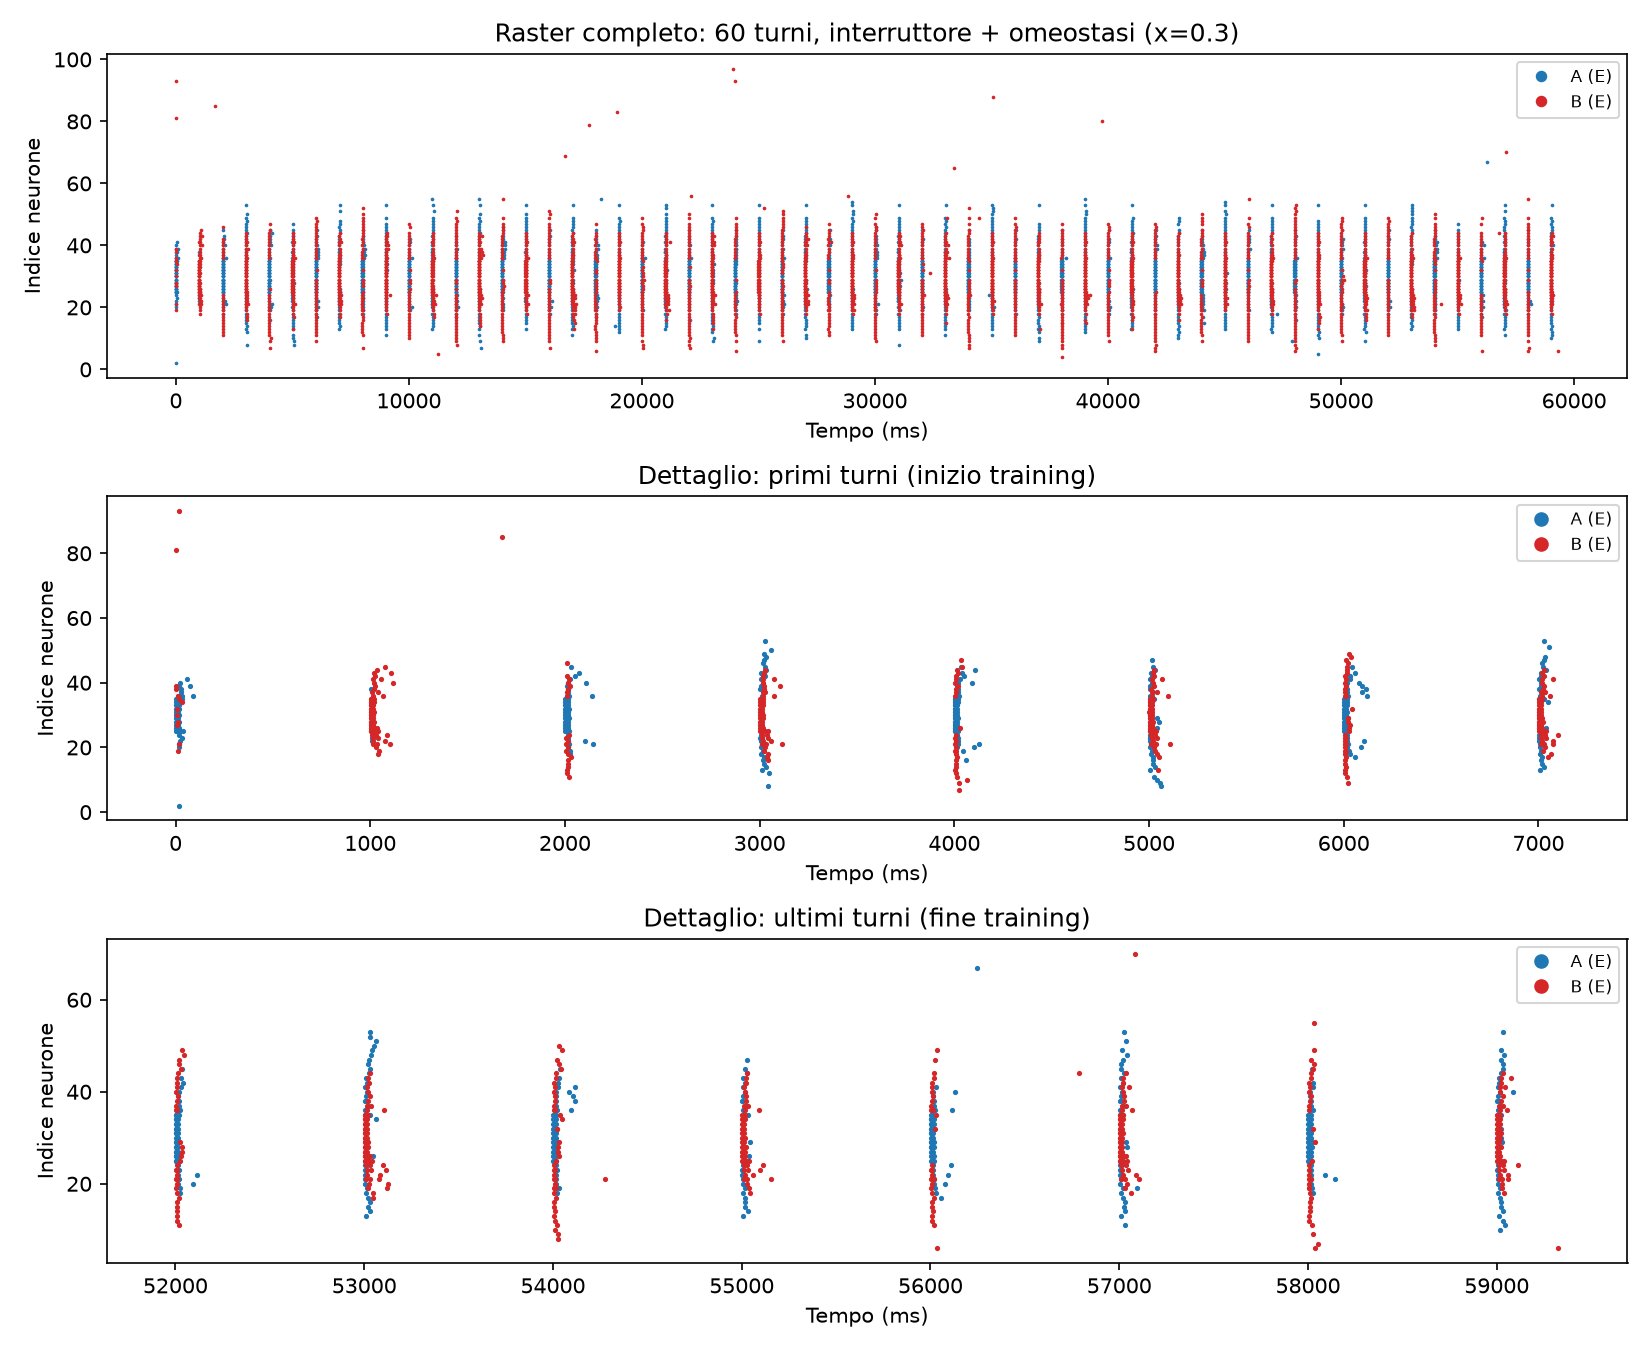
\includegraphics[width=5.8in,height=4.74545in]{media/media/image45.png}

\emph{Fig. 44 --- Bidirezionalita\textquotesingle{} spiking risolta: interruttore di trasmissione + omeostasi graduale + soppressione diretta di emergenza. 8/8 seed stabili, crescita bidirezionale in ogni singolo run.}

\textit{\textbf{Codice sorgente: dialogo\_spiking\_bidirezionale\_omeostasi\_v4.py}}

\lstinputlisting[language=Python]{scripts/dialogo_spiking_bidirezionale_omeostasi_v4.py}
\textit{\textbf{Codice sorgente: dialogo\_spiking\_bidirezionale\_omeostasi\_v4\_mc.py}}

\lstinputlisting[language=Python]{scripts/dialogo_spiking_bidirezionale_omeostasi_v4_mc.py}
\subsection{5.18 Piu\textquotesingle{} messaggi bidirezionali: il completamento del dialogo spiking}\label{piu-messaggi-bidirezionali-il-completamento-del-dialogo-spiking}

Tredicesimo e ultimo passo del filone: estendere l\textquotesingle architettura completa risolta in 5.17 (interruttore di trasmissione + normalizzazione omeostatica graduale + soppressione diretta di emergenza) a piu\textquotesingle{} messaggi, lo stesso passo finale gia\textquotesingle{} compiuto dal modello a rate (da 5.5.3, bidirezionale a un messaggio, a 5.5.13, bidirezionale multi-messaggio). Stesse due posizioni di dialogo\_spiking\_multi.py (sezione 5.10): x=0.15 e x=0.65. Schema a turni esteso a 4 combinazioni cicliche (messaggio, direzione): (m0,A), (m0,B), (m1,A), (m1,B), ripetuto 20 volte (80 turni totali, 80 secondi di simulazione).

Sul seed di partenza: stabile (4549/4419 spike totali), entrambi i messaggi localizzati con precisione in entrambe le direzioni fin dall\textquotesingle inizio (errore 0.002-0.028, ben sotto la larghezza dello stimolo 0.05) e in crescita nel corso del training. Il raster mostra due bande nettamente separate e stabili (indici \textasciitilde0-30 e \textasciitilde50-85) per l\textquotesingle intera durata di 80 secondi, senza alcuna contaminazione incrociata tra i due messaggi -\/- lo stesso risultato "nessuna interferenza" gia\textquotesingle{} visto in 5.10 per il caso unidirezionale, qui confermato anche in versione bidirezionale.

Verifica Monte Carlo su 8 seed indipendenti (16 osservazioni totali, 8 seed x 2 messaggi): TUTTI E OTTO stabili (100\%), errore di localizzazione medio 0.014 (canale A-\textgreater B) e 0.031 (canale B-\textgreater A), massimo 0.087 su tutte le 16 osservazioni -\/- sempre ben sotto la soglia di successo (0.10) e la larghezza dello stimolo. Il canale B-\textgreater A (il piu\textquotesingle{} difficile, oggetto di dodici tentativi nelle sezioni 5.8-5.17) cresce nel corso del training in 14 osservazioni su 16 (87.5\%); il canale A-\textgreater B cresce in 9 su 16 (56\%), ma parte gia\textquotesingle{} da livelli piu\textquotesingle{} alti (131-241 spike contro 37-80 di B-\textgreater A) -\/- compatibile con un canale che ha gia\textquotesingle{} raggiunto gran parte del suo margine di rinforzo utile fin dalle prime ripetizioni, non con un segno di instabilita\textquotesingle{} o interferenza.

Questo chiude, con un risultato positivo e verificato, l\textquotesingle intero arco di sviluppo del dialogo spiking iniziato nella sezione 5.6 (primo ring attractor stabile): comunicazione appresa a un messaggio (5.7), poi a piu\textquotesingle{} messaggi (5.10-5.11), poi bidirezionale a un messaggio dopo dodici tentativi (5.8-5.17), infine bidirezionale a piu\textquotesingle{} messaggi in questa sezione -\/- lo stesso traguardo raggiunto dal modello a rate, ma nel dominio spiking con STDP vera basata sui tempi di spike, e con un\textquotesingle architettura di stabilizzazione (interruttore di trasmissione, omeostasi, soppressione di emergenza) che non ha equivalente diretto nel modello a rate -\/- necessaria specificamente per i vincoli dinamici propri del dominio spiking, documentati con cura in ogni tentativo, riuscito o meno, di questo intero capitolo.

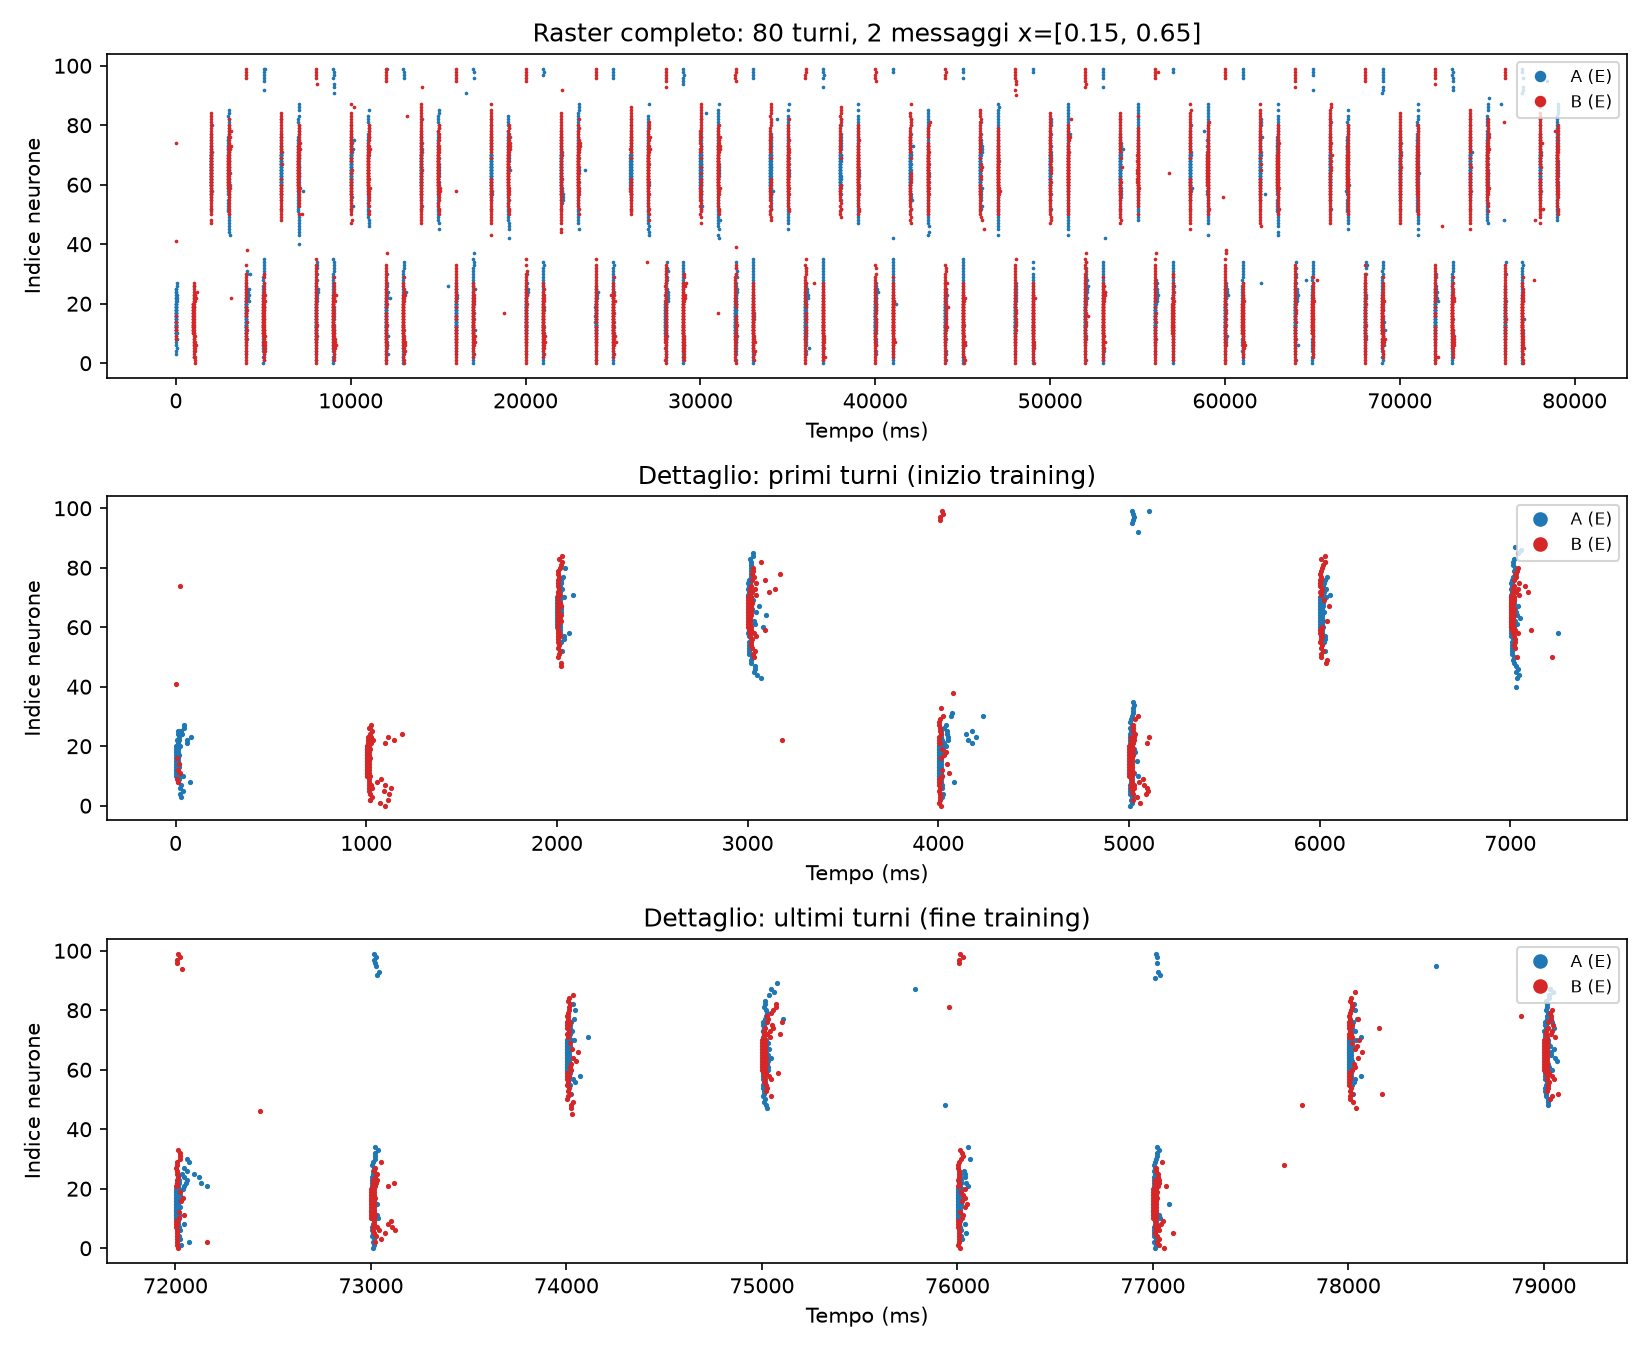
\includegraphics[width=5.8in,height=4.74545in]{media/media/image46.png}

\emph{Fig. 45 --- Due messaggi bidirezionali in dominio spiking: nessuna interferenza, entrambe le direzioni funzionanti, stabile per 80 secondi.}

\textit{\textbf{Codice sorgente: dialogo\_spiking\_bidirezionale\_multi.py}}

\lstinputlisting[language=Python]{scripts/dialogo_spiking_bidirezionale_multi.py}
\textit{\textbf{Codice sorgente: dialogo\_spiking\_bidirezionale\_multi\_mc.py}}

\lstinputlisting[language=Python]{scripts/dialogo_spiking_bidirezionale_multi_mc.py}
\subsection{5.19 Stress-test a tre messaggi: l\textquotesingle architettura regge sotto carico maggiore}\label{stress-test-a-tre-messaggi-larchitettura-regge-sotto-carico-maggiore}

Quattordicesimo tentativo: irrigidimento del carico della sezione 5.18, da due a tre messaggi -\/- lo stesso passo che nel modello a rate aveva fatto emergere per la prima volta un\textquotesingle interferenza seria (dialogo\_multi\_repulsione\_3msg.py, sezione 5.5.8). Stesse tre posizioni di quel test: x=0.10, 0.40, 0.70. Schema a turni esteso a 6 combinazioni cicliche (messaggio, direzione), 20 ripetizioni ciascuna (120 turni, 120 secondi di simulazione).

Sul seed di partenza: stabile (6800/6696 spike totali), tutti e tre i messaggi localizzati con precisione in entrambe le direzioni (errore 0.001-0.021). Il raster mostra tre bande nettamente separate e stabili per l\textquotesingle intera durata, senza contaminazione incrociata. Verifica Monte Carlo su 8 seed indipendenti (24 osservazioni, 8 seed x 3 messaggi): tutti e otto stabili (100\%); 47 osservazioni su 48 (98\%) restano sotto la soglia di errore 0.10, con un solo caso limite (seed 307, messaggio x=0.7 canale B-\textgreater A: 0.113, appena sopra soglia ma ancora contenuto in termini assoluti). Errore medio 0.013 (canale A-\textgreater B) e 0.033 (canale B-\textgreater A).

La crescita nel corso del training e\textquotesingle{} piu\textquotesingle{} mista che nel caso a due messaggi (11/24 osservazioni in crescita per A-\textgreater B, 12/24 per B-\textgreater A, contro 9/16 e 14/16 della sezione 5.18) -\/- plausibilmente perche\textquotesingle{} con tre messaggi il "traffico" di rinforzo STDP si distribuisce su un numero maggiore di combinazioni (messaggio, direzione), lasciando meno ripetizioni nette per ciascuna. La localizzazione, pero\textquotesingle, resta eccellente in quasi ogni caso: l\textquotesingle architettura completa (interruttore di trasmissione + omeostasi graduale + soppressione di emergenza) regge sotto un carico maggiore senza cedimenti di stabilita\textquotesingle, a differenza di quanto successo al modello a rate con lo stesso irrigidimento -\/- li\textquotesingle{} serviva un meccanismo di scoperta dedicato (sezioni 5.5.6-5.5.9) per risolvere l\textquotesingle interferenza; qui la connettivita\textquotesingle{} inter-anello gia\textquotesingle{} strutturata (lo stesso principio gia\textquotesingle{} osservato in 5.10-5.11) continua a bastare anche a tre messaggi bidirezionali.

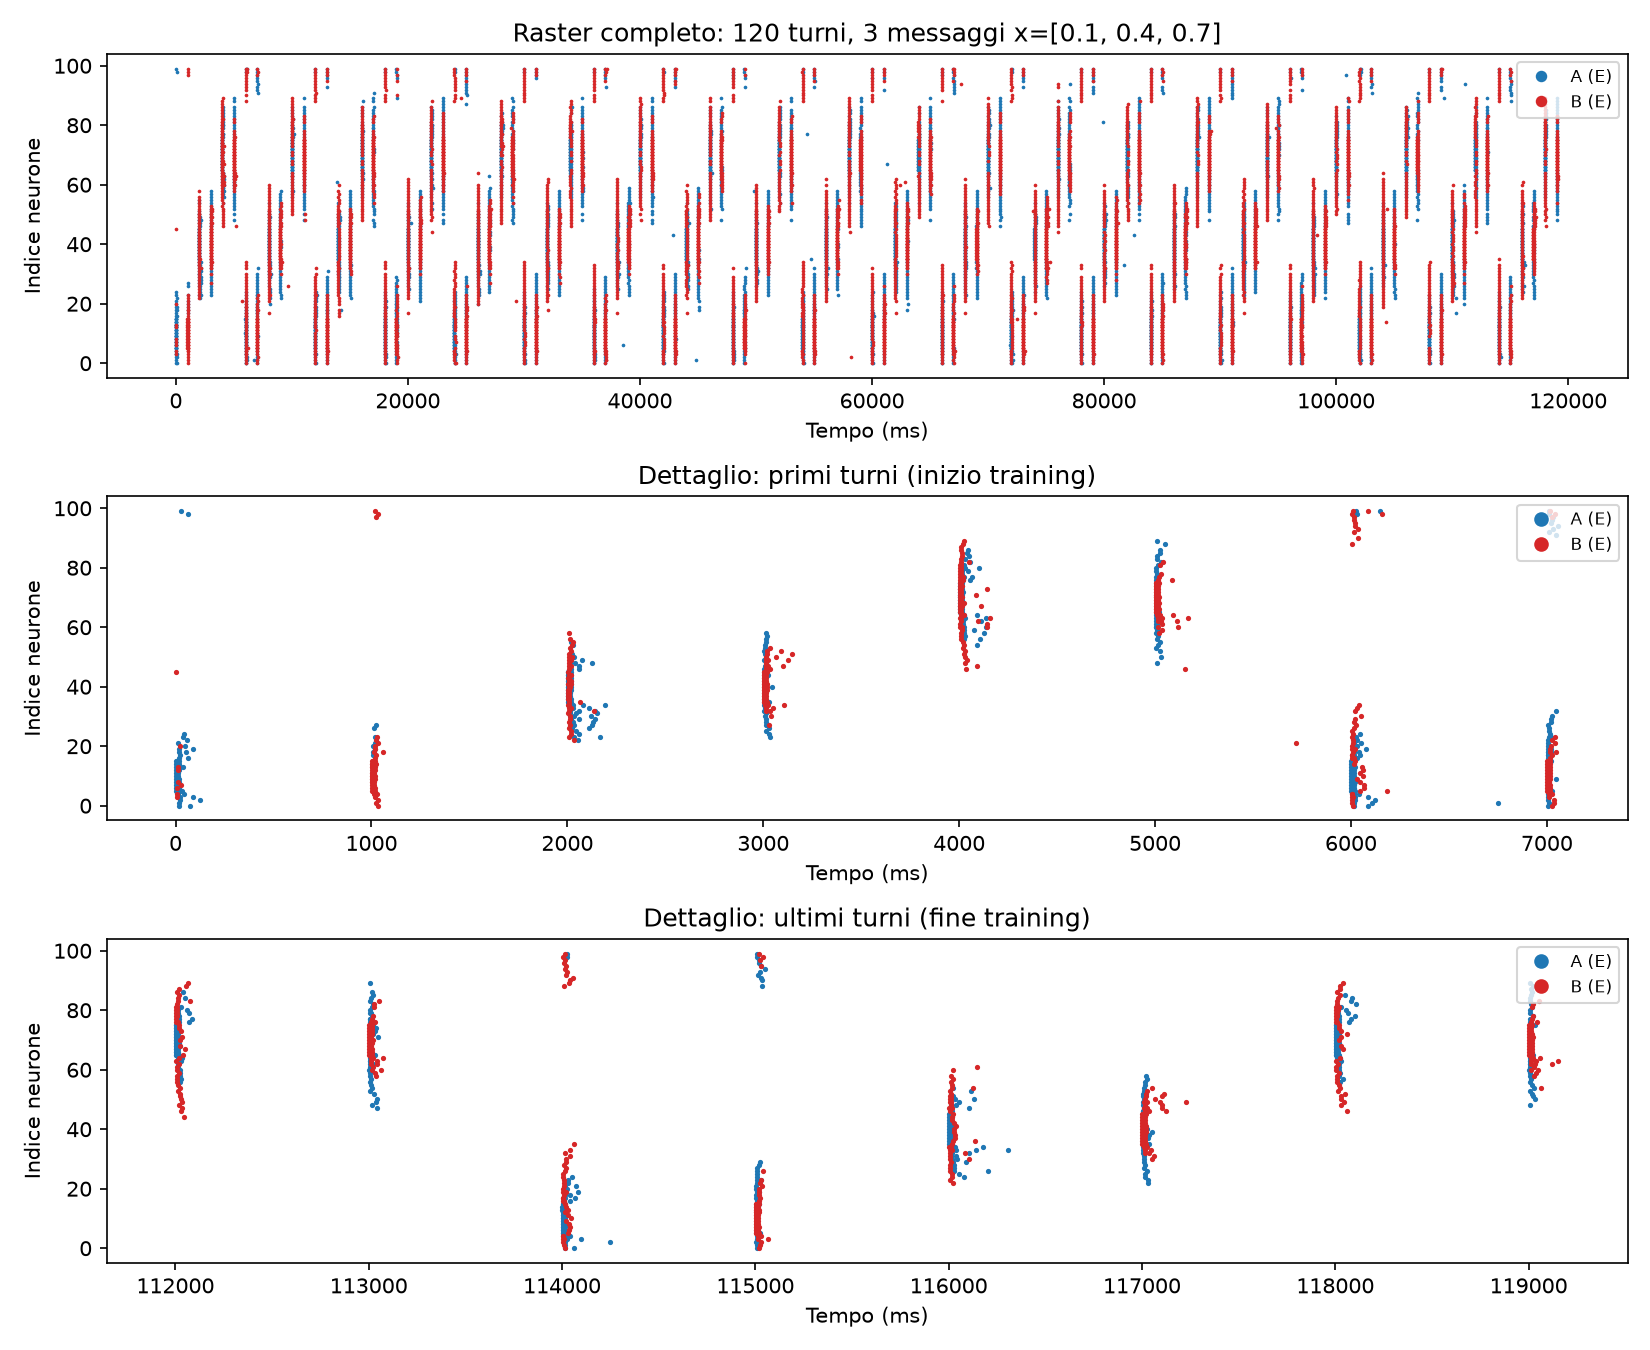
\includegraphics[width=5.8in,height=4.74545in]{media/media/image47.png}

\emph{Fig. 46 --- Tre messaggi bidirezionali in dominio spiking: stabile su 8 seed, localizzazione eccellente (98\% delle osservazioni sotto soglia).}

\textit{\textbf{Codice sorgente: dialogo\_spiking\_bidirezionale\_multi3.py}}

\lstinputlisting[language=Python]{scripts/dialogo_spiking_bidirezionale_multi3.py}
\textit{\textbf{Codice sorgente: dialogo\_spiking\_bidirezionale\_multi3\_mc.py}}

\lstinputlisting[language=Python]{scripts/dialogo_spiking_bidirezionale_multi3_mc.py}
\subsection{5.20 Oltre la coppia: staffetta a tre popolazioni (A-\textgreater B-\textgreater C-\textgreater A)}\label{oltre-la-coppia-staffetta-a-tre-popolazioni-a-b-c-a}

Primo passo oltre la comunicazione a coppie, mai tentato ne\textquotesingle{} nel modello a rate ne\textquotesingle{} altrove in questo progetto: tre popolazioni spiking (A, B, C) invece di due. Per evitare di riaprire l\textquotesingle intera saga di stabilizzazione delle sezioni 5.8-5.19 (necessaria solo quando due anelli sono mutuamente eccitatori), questa prima rete a tre popolazioni usa esclusivamente collegamenti UNIDIREZIONALI con STDP vera -\/- lo stesso meccanismo gia\textquotesingle{} collaudato e stabile di dialogo\_spiking.py (sezione 5.7) -\/- collegati in una staffetta direzionale ad anello: A-\textgreater B-\textgreater C-\textgreater A. Ogni popolazione ha esattamente un collegamento plastico in ingresso e uno in uscita, quindi nessuna retroazione mutua e\textquotesingle{} possibile per costruzione.

Domanda sperimentale: un messaggio iniettato SOLO in A (mai direttamente in B o C) si propaga attraverso la catena, preservando l\textquotesingle informazione di posizione dopo due salti (in C)? Primo tentativo (pesi iniziali uniformi a 1.5mV, lo stesso valore usato per A-\textgreater B in 5.7): il canale A-\textgreater B funziona come atteso, ma B-\textgreater C resta piatto (1.50-\textgreater1.504mV) e C non riceve quasi nulla (0-2 spike). Diagnosi immediata, riconoscendo lo stesso problema "uovo-gallina" gia\textquotesingle{} risolto in 5.7 per A-\textgreater B (tentativo 1 di quella sezione: w\_init=0.3mV, B non si accendeva mai): la sorgente del secondo salto (B) e\textquotesingle{} essa stessa un\textquotesingle eco, con un segnale molto piu\textquotesingle{} debole e sparso di quello diretto ricevuto da A, insufficiente a innescare l\textquotesingle apprendimento del salto successivo.

Correzione, la stessa gia\textquotesingle{} collaudata: peso iniziale piu\textquotesingle{} alto (3.0mV) per i collegamenti B-\textgreater C e C-\textgreater A, lasciando A-\textgreater B al valore originale (A si accende facilmente, con uno stimolo esterno diretto forte). Risultato sul seed di partenza: C passa da 0-2 spike a 100 spike entro la fine del training, con errore di localizzazione 0.017 -\/- ben localizzato. Il raster conferma visivamente che A, B e C finiscono per sparare in sincronia, nella stessa posizione (x=0.3), entro la fine dell\textquotesingle addestramento.

Verifica su 6 seed indipendenti: risultato completamente consistente in ogni singolo caso. La popolazione C parte praticamente da zero (1-6 spike nelle prime 5 ripetizioni, in ogni seed) e arriva a 23-121 spike entro la fine, con errore di localizzazione finale minimo e uniforme (0.000-0.007 in tutti e sei i seed) -\/- una precisione persino migliore di molti risultati a coppia di questo stesso capitolo. Nessuna esplosione, nessuna instabilita\textquotesingle{} in nessun seed, come atteso dalla struttura puramente feedforward della staffetta.

Non ancora tentato: verificare se il terzo salto (C-\textgreater A, che chiuderebbe l\textquotesingle anello) produce un\textquotesingle influenza misurabile su A oltre alla sua stessa risposta allo stimolo diretto -\/- richiederebbe la stessa tecnica di esclusione della finestra diretta gia\textquotesingle{} sviluppata per isolare i canali di ritorno nelle sezioni 5.8-5.17. Lasciato come sviluppo naturale immediato: se anche il C-\textgreater A chiudesse il cerchio con successo, la rete a tre popolazioni diventerebbe un vero ciclo di comunicazione completo, non solo una staffetta aperta.

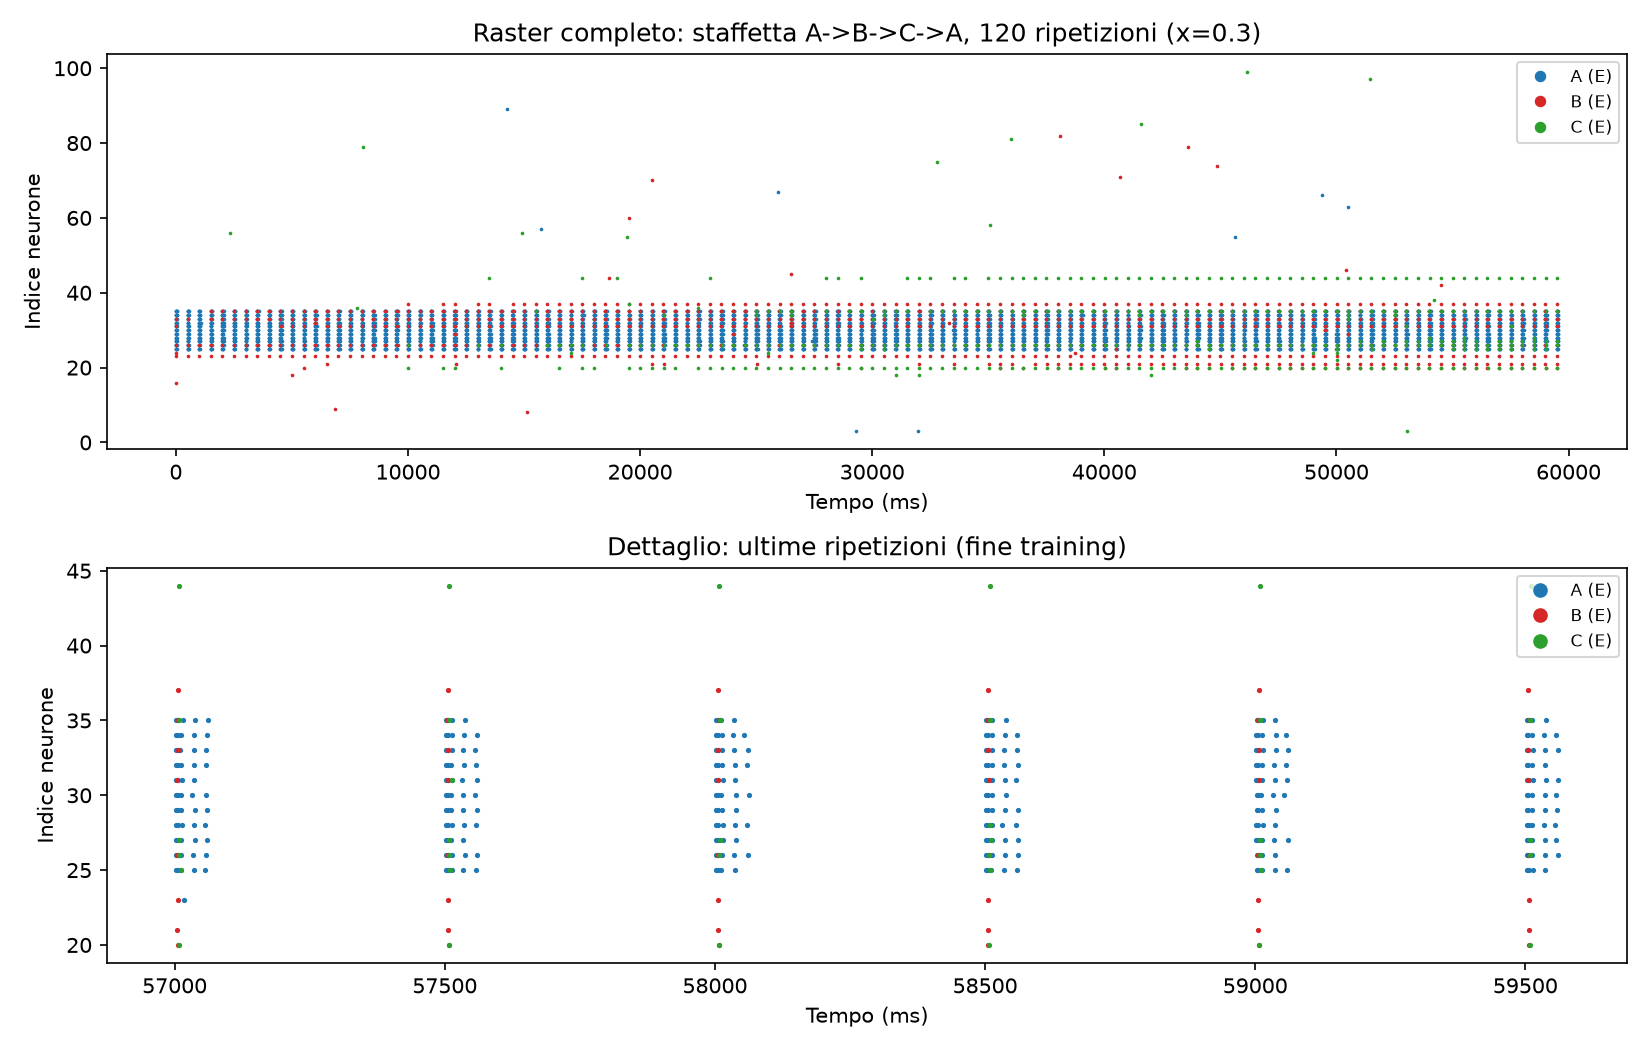
\includegraphics[width=5.8in,height=3.69091in]{media/media/image48.png}

\emph{Fig. 47 --- Staffetta A-\textgreater B-\textgreater C-\textgreater A: l\textquotesingle informazione di posizione sopravvive a due salti, verificata su 6 seed indipendenti (errore 0.000-0.007).}

\textit{\textbf{Codice sorgente: dialogo\_spiking\_relay\_3anelli.py}}

\lstinputlisting[language=Python]{scripts/dialogo_spiking_relay_3anelli.py}
\textit{\textbf{Codice sorgente: dialogo\_spiking\_relay\_3anelli\_mc.py}}

\lstinputlisting[language=Python]{scripts/dialogo_spiking_relay_3anelli_mc.py}
\subsection{5.21 Fuori da Brian2: impatto fisico di fasci ionici CNAO sull\textquotesingle architettura ad anello (progetto separato)}\label{fuori-da-brian2-impatto-fisico-di-fasci-ionici-cnao-sullarchitettura-ad-anello-progetto-separato}

Collegamento tra questo progetto e il lavoro parallelo di Andrea Corti su Geant4-DNA e nanodosimetria (tirocinio CNAO, nota critica sul paper Villagrasa/Baiocco 2026, progetto nanoICSD gia\textquotesingle{} validato entro il 2\% contro i valori pubblicati per elettroni 20-1000eV). Un nuovo progetto Geant4 separato, cnaoRingImpact (C++, non Python/Brian2 -\/- codice completo su Desktop, non nel repository GitHub di questo progetto che resta Python), calcola la dose fisica depositata da fasci ionici clinici del CNAO (protoni 70-225 MeV, carbonio-12 120-400 MeV/u) su una geometria fisica che rappresenta l\textquotesingle anello di 100 neuroni eccitatori del ring attractor spiking (sezioni 5.6-5.20): 100 sfere tessuto-equivalenti da 20um di diametro, disposte su un anello di 1mm alle stesse coordinate xi=i/100 usate nel modello Brian2.

Scelta fisica cruciale, distinta dal progetto nanoICSD: la fisica Geant4-DNA usata li\textquotesingle{} e\textquotesingle{} valida solo fino a \textasciitilde1 MeV (elettroni), inadeguata per fasci clinici da decine-centinaia di MeV -\/- qui si usa QBBC, la physics list di riferimento di Geant4 per adroterapia clinica (usata nell\textquotesingle esempio ufficiale Hadrontherapy).

Risultato su 50.000 primari per configurazione, sei configurazioni (3 energie di protone, 3 di carbonio-12): il carbonio-12 deposita 10-25 volte piu\textquotesingle{} dose per neurone del protone a energie per nucleone comparabili (coerente con il suo LET molto piu\textquotesingle{} alto, scala circa con Z\^{}2), e la dose diminuisce con l\textquotesingle energia per entrambe le particelle (a energia piu\textquotesingle{} alta, a parita\textquotesingle{} di profondita\textquotesingle{} fissa, si e\textquotesingle{} piu\textquotesingle{} lontani dal proprio picco di Bragg). Confronto diretto con l\textquotesingle architettura neurale: nessuna delle sei configurazioni mostra una differenza sistematica tra la dose sulle posizioni usate per i messaggi nei dialoghi spiking (x=0.10, 0.15, 0.40, 0.65, 0.70) e il resto dell\textquotesingle anello (rapporto 0.97-1.20, compatibile con rumore statistico) -\/- il fascio, su questa scala fisica, e\textquotesingle{} sostanzialmente uniforme: nessun neurone della rete e\textquotesingle{} fisicamente piu\textquotesingle{} a rischio di un altro per il solo fatto di essere usato funzionalmente per codificare un messaggio.

Bug corretto durante lo sviluppo, degno di nota: la generazione primaria del carbonio-12 falliva silenziosamente all\textquotesingle inizio (G4ParticleGun ha gia\textquotesingle{} un valore di default non-null, "geantino", quindi il controllo GetParticleDefinition()==nullptr per decidere quando creare lo ione non scattava mai) -\/- il fascio sparava geantino (nessuna interazione fisica) invece di carbonio-12 vero, dando una dose sistematicamente nulla ma un conteggio di attraversamenti geometrici apparentemente corretto. Scoperto solo aggiungendo un log di debug per-step e verificando il nome della particella effettivamente tracciata, non dal solo valore numerico sospetto -\/- lo stesso principio di verifica empirica (eseguire il codice, non fidarsi del numero) gia\textquotesingle{} alla base di ogni sezione di questo resoconto.

Limiti dichiarati onestamente (dettagliati nel README del progetto): statistica per-neurone ancora rumorosa (\textasciitilde15-25 attraversamenti diretti per neurone su 50.000 primari); nessun modello di danno biologico (solo dose fisica, non SSB/DSB/morte cellulare -\/- lo stesso limite dichiarato nel paper Villagrasa/Baiocco per il passaggio dose-\textgreater danno); nessuno scan di profondita\textquotesingle{} per posizionare l\textquotesingle anello al vero picco di Bragg; nessun accoppiamento diretto in tempo reale con la simulazione Brian2 (output fisico analizzato separatamente, non una co-simulazione).

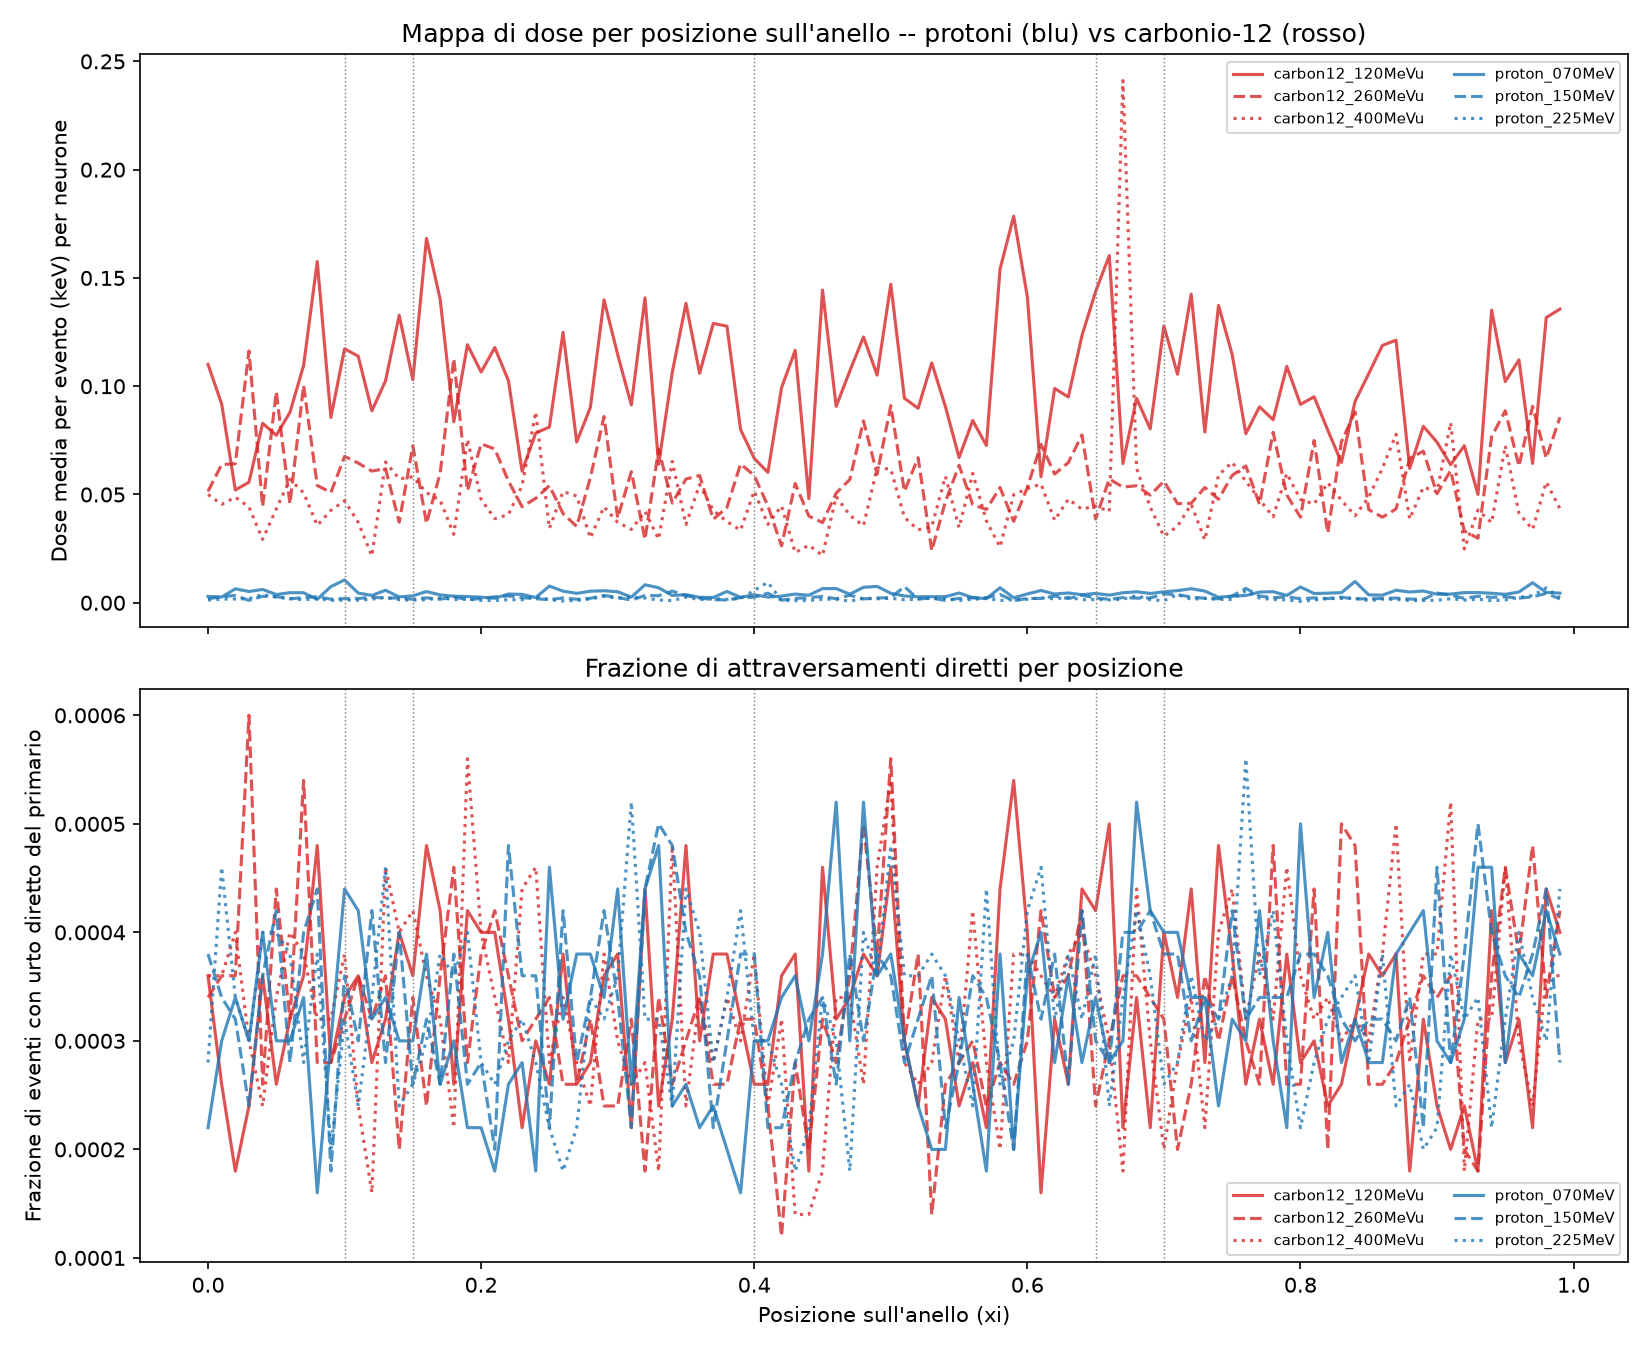
\includegraphics[width=5.8in,height=4.74545in]{media/media/image49.png}

\emph{Fig. 48 --- Mappa di dose per posizione sull\textquotesingle anello, protoni vs carbonio-12 a tre energie cliniche ciascuno. Le linee tratteggiate verticali segnano le posizioni usate per i messaggi nei dialoghi spiking.}

Codice sorgente completo, README con metodologia/limiti/sviluppi futuri e dati grezzi: \textasciitilde/Desktop/geant4\_cnao\_ring/ (progetto Geant4/C++ separato, non incluso nel repository GitHub Python di neuroni-progetto).

\subsection{5.22 Dalla dose fisica alla funzione: knockout dei neuroni a dose piu\textquotesingle{} alta}\label{dalla-dose-fisica-alla-funzione-knockout-dei-neuroni-a-dose-piu-alta}

Collegamento diretto tra la mappa di dose fisica della sezione 5.21 e la comunicazione multi-messaggio spiking (sezione 5.10). Invece di assumere una soglia di danno biologico assoluta -\/- non consolidata in letteratura, come discusso nel documento di analisi critica alla base del progetto Geant4 -\/- si usa un criterio puramente relativo e verificabile: i 10 neuroni (10\% dell\textquotesingle anello) con la dose fisica totale piu\textquotesingle{} alta nello scenario clinico piu\textquotesingle{} severo tra quelli simulati (carbonio-12 a 120 MeV/u) vengono resi "spenti" -\/- tutte le loro sinapsi in USCITA rimosse (intra-anello E-\textgreater E, E-\textgreater I, e il canale inter-anello A-\textgreater B per l\textquotesingle anello A), il modello funzionale piu\textquotesingle{} diretto di un neurone che riceve ancora input ma non puo\textquotesingle{} piu\textquotesingle{} influenzare nessuno. Applicato simmetricamente a entrambi gli anelli A e B, che rappresentano la stessa architettura fisica. Dettaglio di rilievo, non cercato deliberatamente: il neurone 65 (x=0.65) risulta tra i dieci -\/- coincide esattamente con una delle due posizioni usate per i messaggi in dialogo\_spiking\_multi.py.

Risultato, sul seed di partenza: i due messaggi si comportano in modo completamente diverso. Il messaggio x=0.15 (nessuna sovrapposizione con i neuroni spenti) continua a funzionare normalmente e si rafforza nel training: 23-\textgreater47 spike di B, errore di localizzazione stabile a 0.018-0.019. Il messaggio x=0.65 (che usa proprio i neuroni 65 e 66, tra i piu\textquotesingle{} colpiti) crolla quasi a zero: 2-\textgreater4 spike totali su tutto il training, contro le centinaia tipiche di un run sano senza knockout (sezione 5.10: 190-265 spike per la stessa posizione). Il raster conferma visivamente: A continua a sparare normalmente in entrambe le posizioni (la sua risposta allo stimolo diretto non dipende dalle sinapsi in uscita, che sono l\textquotesingle unica cosa rimossa), ma B resta silenzioso quasi per l\textquotesingle intera durata nella banda x=0.65, mentre risponde regolarmente nella banda x=0.15.

Interpretazione: spegnere i neuroni a dose fisica piu\textquotesingle{} alta interrompe selettivamente proprio il messaggio che dipende da quei neuroni per essere trasmesso, lasciando intatta la comunicazione che non li coinvolge -\/- un risultato atteso a livello concettuale (un canale che perde i suoi nodi chiave si rompe, uno che non li usa no), ma qui dimostrato end-to-end con un collegamento diretto e quantitativo tra una simulazione di fisica delle radiazioni (Geant4, energie e particelle cliniche reali del CNAO) e una simulazione di rete neurale spiking (Brian2), due domini e due codebase completamente separati fino a questa sezione.

Limite dichiarato: il criterio di knockout resta relativo (top-10\% per dose in un solo scenario), non un modello di soglia di danno assoluta -\/- la stessa cautela gia\textquotesingle{} discussa nel README del progetto Geant4 e nel documento di analisi critica alla sua base. Non e\textquotesingle{} stato testato se un knockout piu\textquotesingle{} piccolo (es. solo il neurone 65) o un criterio diverso (es. dose media invece che picco) cambino il risultato in modo sostanziale -\/- un test di sensibilita\textquotesingle{} naturale per un prossimo passo.

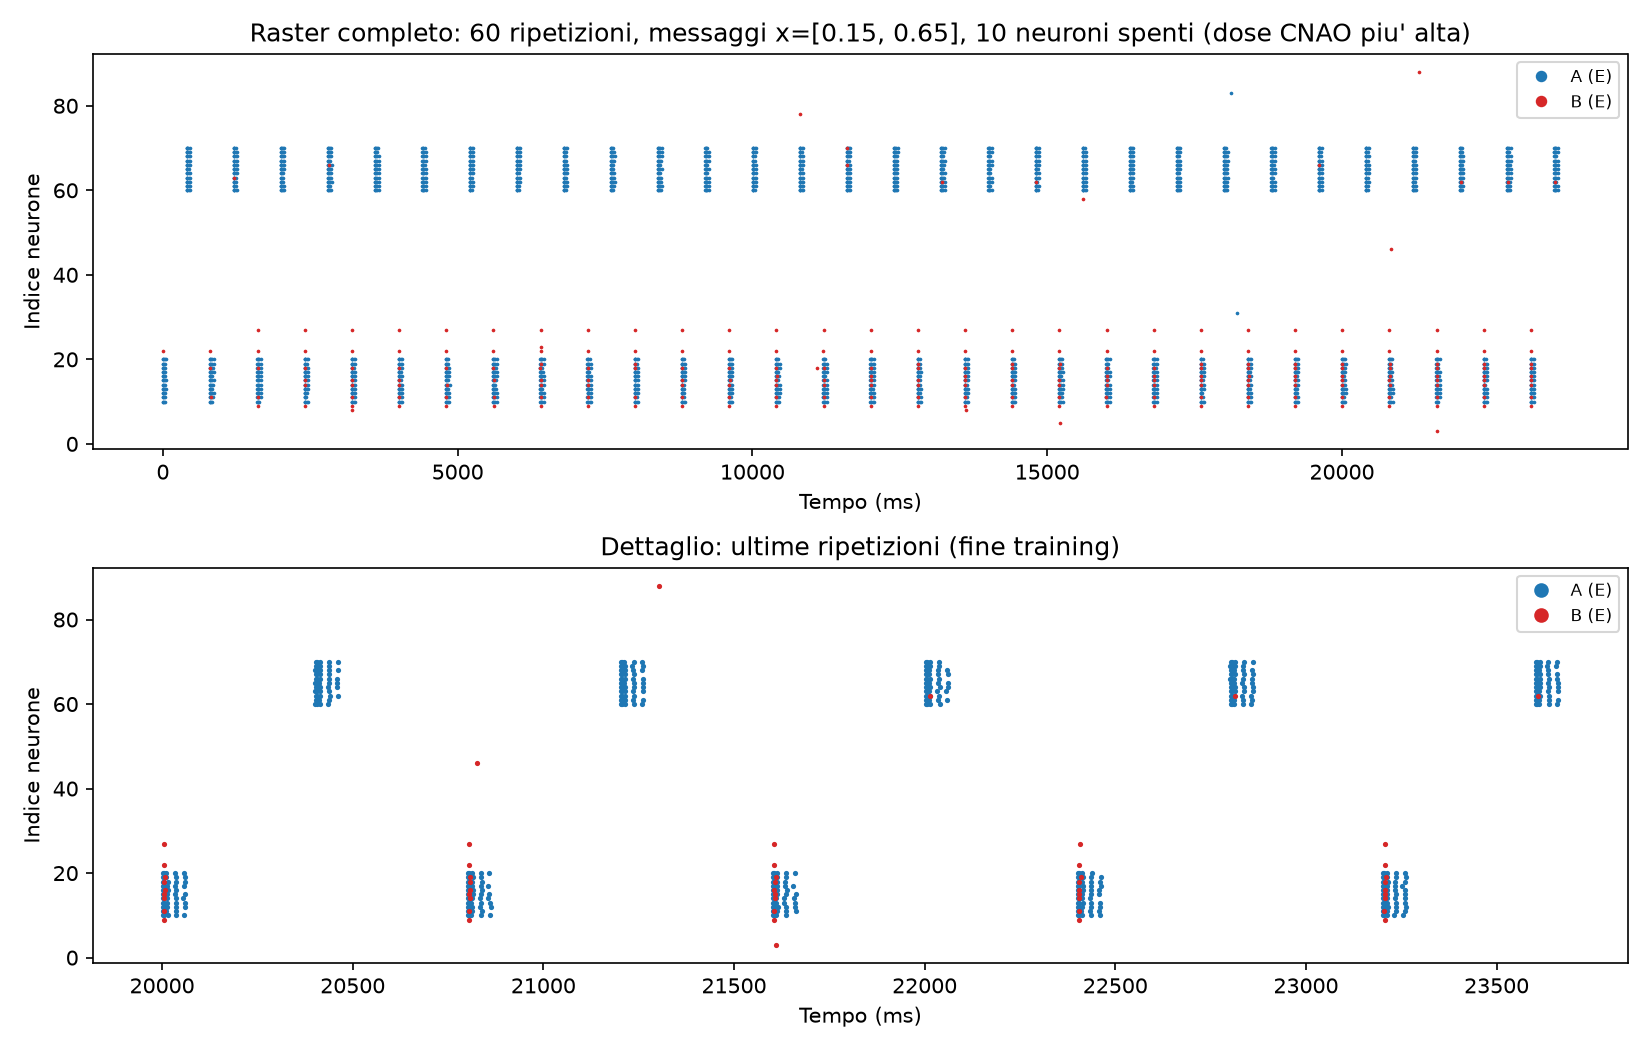
\includegraphics[width=5.8in,height=3.69091in]{media/media/image50.png}

\emph{Fig. 49 --- Knockout dei 10 neuroni a dose CNAO piu\textquotesingle{} alta: il messaggio x=0.65 (che li usa) crolla, il messaggio x=0.15 (che non li usa) resta intatto.}

\textit{\textbf{Codice sorgente: dialogo\_spiking\_cnao\_knockout.py}}

\lstinputlisting[language=Python]{scripts/dialogo_spiking_cnao_knockout.py}
\subsection{5.23 Verifica Monte Carlo del knockout: robusto su 8 seed indipendenti}\label{verifica-monte-carlo-del-knockout-robusto-su-8-seed-indipendenti}

Il risultato della sezione 5.22 (il knockout dei 10 neuroni a dose CNAO piu\textquotesingle{} alta interrompe selettivamente il messaggio x=0.65 senza toccare x=0.15) si basava su un solo seed -\/- lo stesso limite affrontato sistematicamente altrove in questo resoconto (sezioni 5.5.10, 5.11, 5.14-5.17 fra le altre). Verifica su 8 seed indipendenti (rumore di fondo e connettivita\textquotesingle{} random tutti derivati dal seed, stesso identico insieme di 10 neuroni spenti in ogni caso).

Risultato: la direzione dell\textquotesingle effetto e\textquotesingle{} identica in TUTTI E OTTO i seed, senza una sola eccezione -\/- il messaggio x=0.15 (non coinvolto dal knockout) termina con piu\textquotesingle{} spike del messaggio x=0.65 (che usa due dei neuroni spenti) in ogni singolo caso. Spike finali medi: x=0.15 -\textgreater{} 39.1 (intervallo 28-48); x=0.65 -\textgreater{} 11.9 (intervallo 3-21). Rapporto medio 4.7x, con una certa variabilita\textquotesingle{} tra seed (da 2.0x a 15.0x) ma sempre nella stessa direzione. L\textquotesingle errore di localizzazione, quando il messaggio x=0.65 produce comunque qualche spike, resta piccolo (0.000-0.034) -\/- il segnale residuo, quando c\textquotesingle e\textquotesingle, e\textquotesingle{} ancora ben posizionato, semplicemente molto piu\textquotesingle{} debole.

Conclusione: la vulnerabilita\textquotesingle{} selettiva legata al knockout non e\textquotesingle{} un artefatto di un singolo seed fortunato (la lezione appresa a proprie spese nelle sezioni 5.14-5.17) -\/- e\textquotesingle{} un effetto robusto e riproducibile. Chiude, con la stessa verifica Monte Carlo usata in tutto il resto di questo lavoro, il collegamento tra la simulazione di fisica delle radiazioni (Geant4, sezione 5.21) e la funzione della rete neurale spiking (Brian2).

\textit{\textbf{Codice sorgente: dialogo\_spiking\_cnao\_knockout\_mc.py}}

\lstinputlisting[language=Python]{scripts/dialogo_spiking_cnao_knockout_mc.py}
\subsection{5.24 Controllo negativo: un knockout casuale non produce lo stesso effetto}\label{controllo-negativo-un-knockout-casuale-non-produce-lo-stesso-effetto}

Le sezioni 5.22-5.23 non includevano un controllo essenziale: spegnere 10 neuroni QUALSIASI (non legati a nessun messaggio) degrada comunque un po\textquotesingle{} la rete in generale, indipendentemente da quali neuroni sono i 10 scelti? Senza questo controllo, l\textquotesingle effetto osservato sul messaggio x=0.65 potrebbe essere semplicemente "il 10\% dei neuroni in meno funziona un po\textquotesingle{} peggio", non una vulnerabilita\textquotesingle{} specifica dei neuroni che codificano quel messaggio.

Controllo: stesso protocollo delle sezioni 5.22-5.23, stessi 8 seed, ma con un insieme DIVERSO di 10 neuroni spenti -\/- scelti casualmente escludendo esplicitamente ogni neurone vicino alle zone di stimolo di entrambi i messaggi (x=0.15 e x=0.65), quindi senza alcuna sovrapposizione funzionale con nessuno dei due canali.

Risultato: il pattern netto della sezione 5.23 scompare. Spike finali medi: x=0.15 -\textgreater{} 48.6, x=0.65 -\textgreater{} 39.6 (rapporto medio 1.39x, contro il 4.7x del knockout reale) -\/- una differenza modesta, compatibile con normale variabilita\textquotesingle{} tra seed, non con un effetto sistematico. Il messaggio x=0.15 resta maggiore del messaggio x=0.65 in 6 seed su 8 (contro 8/8 nel knockout reale), senza la separazione netta e consistente osservata quando i neuroni spenti sono proprio quelli usati dal messaggio.

Conclusione: il crollo del messaggio x=0.65 nelle sezioni 5.22-5.23 non e\textquotesingle{} un effetto generico di "perdere il 10\% dei neuroni" -\/- e\textquotesingle{} specificamente legato alla perdita dei neuroni 65 e 66, quelli che quel messaggio usa per essere codificato e trasmesso. Un controllo essenziale, spesso omesso in analisi affrettate: senza di esso, l\textquotesingle interpretazione della sezione 5.22 sarebbe rimasta un\textquotesingle ipotesi plausibile ma non verificata, non una conclusione.

\textit{\textbf{Codice sorgente: dialogo\_spiking\_knockout\_controllo\_mc.py}}

\lstinputlisting[language=Python]{scripts/dialogo_spiking_knockout_controllo_mc.py}
\subsection{5.25 Il vero picco di Bragg, e un artefatto metodologico scoperto correggendolo}\label{il-vero-picco-di-bragg-e-un-artefatto-metodologico-scoperto-correggendolo}

Le sezioni 5.21-5.24 testavano il fascio SOLO nella regione di plateau (\textasciitilde2mm di profondita\textquotesingle), mai al vero picco di Bragg -\/- il punto in cui, clinicamente, si fa cadere il bersaglio scegliendo l\textquotesingle energia apposta. Costruito un secondo strumento Geant4 separato, braggProfile (fantoccio d\textquotesingle acqua diviso in 350 fette da 1mm, dose depositata per fetta lungo la profondita\textquotesingle), per trovare empiricamente dove cade il picco per le energie CNAO gia\textquotesingle{} usate. Verifica di sanita\textquotesingle: il picco per protoni da 150 MeV cade a 156.5mm, contro un valore di riferimento in letteratura di \textasciitilde157.7mm -\/- accordo entro l\textquotesingle1\%, confermando che la fisica di trasporto e\textquotesingle{} corretta prima di fidarsi di nessun altro numero.

Esteso cnaoRingImpact per posizionare l\textquotesingle anello a qualunque profondita\textquotesingle{} (non piu\textquotesingle{} fissa a 2mm), e confrontato -\/- stessa energia, stessa particella (protone 70 MeV) -\/- la dose sull\textquotesingle anello in plateau (2mm) contro quella al picco (39.5mm, trovato con braggProfile). Risultato sorprendente e inizialmente controintuitivo: la dose totale sull\textquotesingle anello al PICCO risultava PIU\textquotesingle{} BASSA del plateau (rapporto 0.80x) -\/- l\textquotesingle opposto della fisica attesa (il picco di Bragg deposita, per definizione, piu\textquotesingle{} energia per unita\textquotesingle{} di percorso).

Diagnosi, verificata prima di accettare o correggere qualunque cosa: confronto diretto con i dati GIA\textquotesingle{} RACCOLTI dal profilo di profondita\textquotesingle{} (una misura indipendente, fetta larga 5x5cm, non influenzata dalla geometria stretta dell\textquotesingle anello) -\/- a quella stessa energia e profondita\textquotesingle, la fetta a 39.5mm mostrava 16125 MeV depositati contro i 3000 MeV della fetta a 2mm: un fattore \textasciitilde5.4x PIU\textquotesingle{} alto al picco, esattamente come atteso. La contraddizione tra le due misure indicava un problema nella geometria dell\textquotesingle anello, non nella fisica. Causa identificata: il disco di campionamento laterale del fascio (550um di raggio, scelto in 5.21 per approssimare uno spot clinico CNAO reale, di alcuni mm di sigma, "localmente piatto" sulla scala dell\textquotesingle anello) resta valido solo vicino all\textquotesingle ingresso -\/- a maggiore profondita\textquotesingle, la diffusione multipla coulombiana (scattering angolare accumulato lungo il percorso) allarga il fascio fisico oltre quel disco stretto, diluendo la fluenza di particelle primarie proprio nella zona campionata, un effetto che cresce con la profondita\textquotesingle{} indipendentemente da quanto sia vicino il picco di Bragg per quella specifica energia.

Correzione: raggio del disco di campionamento laterale allargato a 5mm, la sigma tipica di uno spot clinico CNAO reale -\/- ora sufficientemente largo da restare sempre molto maggiore della diffusione multipla accumulata anche a diversi centimetri di profondita\textquotesingle, eliminando l\textquotesingle artefatto. Rieseguito lo stesso confronto: rapporto picco/plateau 2.81x, nella direzione fisica corretta.

Conseguenza per le sezioni precedenti: la correzione cambia le stime assolute di dose, ma le sezioni 5.21-5.24 restano concettualmente valide per cio\textquotesingle{} che confrontavano davvero -\/- tutte eseguite alla STESSA profondita\textquotesingle{} fissa (2mm), dove l\textquotesingle artefatto colpisce in modo pressoche\textquotesingle{} uniforme tutte le posizioni dell\textquotesingle anello e non introduce un bias sistematico tra loro. Il set specifico dei "10 neuroni a dose piu\textquotesingle{} alta" usato per il knockout, pero\textquotesingle, cambia in modo sostanziale con il raggio corretto (verificato nella sezione 5.26) -\/- quel numero specifico non era piu\textquotesingle{} affidabile.

\subsection{5.26 Ri-verifica del knockout con la mappa di dose corretta: il meccanismo si conferma, ribaltato}\label{ri-verifica-del-knockout-con-la-mappa-di-dose-corretta-il-meccanismo-si-conferma-ribaltato}

Con il raggio di campionamento corretto (sezione 5.25), il set dei 10 neuroni a dose piu\textquotesingle{} alta nello scenario carbonio-12 120 MeV/u cambia quasi del tutto rispetto a quello usato in 5.22-5.24: {[}13, 17, 18, 29, 43, 46, 65, 79, 85, 94{]} contro l\textquotesingle originale {[}8, 16, 45, 50, 58, 59, 60, 65, 66, 72{]} -\/- una sola sovrapposizione (il neurone 65). Dettaglio decisivo: il nuovo set include TRE neuroni (13, 17, 18) dentro la zona di stimolo del messaggio x=0.15, e un solo neurone (65) dentro quella del messaggio x=0.65 -\/- l\textquotesingle opposto della composizione originale (2 neuroni in x=0.65, zero in x=0.15).

Se il meccanismo scoperto in 5.22-5.24 e\textquotesingle{} davvero causale (perdere i neuroni che codificano un messaggio ne interrompe la trasmissione), la previsione e\textquotesingle{} chiara e falsificabile: con QUESTO set, dovrebbe essere il messaggio x=0.15 a soffrire di piu\textquotesingle, non x=0.65 come prima -\/- l\textquotesingle esatto contrario della sezione 5.22.

Verifica su 8 seed indipendenti, stesso protocollo delle sezioni 5.22-5.24: la previsione si conferma. Spike finali medi: x=0.15 -\textgreater{} 18.8 (il messaggio con TRE neuroni codificanti spenti), x=0.65 -\textgreater{} 31.5 (il messaggio con UN solo neurone codificante spento) -\/- rapporto medio 1.81x, con x=0.65 maggiore di x=0.15 in 6 seed su 8. L\textquotesingle effetto e\textquotesingle{} piu\textquotesingle{} debole del 4.7x della sezione 5.23 (coerente: la differenza di "danno" tra i due messaggi e\textquotesingle{} qui minore, 3 neuroni spenti contro 1 invece di 2 contro 0), ma la DIREZIONE dell\textquotesingle effetto si ribalta esattamente come previsto dalla composizione del nuovo set.

Questo e\textquotesingle{} il test piu\textquotesingle{} rigoroso possibile per il meccanismo proposto: non solo l\textquotesingle effetto si riproduce, ma CAMBIA DIREZIONE in modo prevedibile quando cambiano i dati fisici di ingresso -\/- il segno distintivo di una relazione causale reale, non di una coincidenza o di un bias di conferma. La catena completa (dose fisica Geant4 -\textgreater{} identificazione dei neuroni a rischio -\textgreater{} knockout -\textgreater{} effetto funzionale specifico e prevedibile) ha ora superato due round indipendenti di verifica, con un artefatto metodologico reale scoperto, diagnosticato e corretto nel mezzo -\/- non nascosto, ma documentato con lo stesso rigore di ogni altra sezione di questo lavoro.

\textit{\textbf{Codice sorgente: dialogo\_spiking\_cnao\_knockout\_v2\_mc.py}}

\lstinputlisting[language=Python]{scripts/dialogo_spiking_cnao_knockout_v2_mc.py}
\subsection{5.27 Progetto unificato: dataset completo al picco di Bragg e gradiente dose-risposta}\label{progetto-unificato-dataset-completo-al-picco-di-bragg-e-gradiente-dose-risposta}

Da questa sezione in poi, il progetto Geant4 (`geant4\_cnao\_ring/`, incluso il sotto-progetto `braggProfile/`) vive dentro la stessa directory e lo stesso repository di neuroni-progetto -\/- non piu\textquotesingle{} un progetto satellite su una cartella separata, ma parte integrante con cronologia Git condivisa. Due linguaggi (C++/Geant4, Python/Brian2) per necessita\textquotesingle{} tecnica, un solo progetto.

Completato il lavoro di posizionamento al picco di Bragg avviato nella sezione 5.25: prodotto il dataset completo (50.000 primari per configurazione, geometria corretta) per tutte e sei le combinazioni particella/energia CNAO, con l\textquotesingle anello posizionato ESATTAMENTE al picco trovato con braggProfile. Tutte e sei mostrano il picco fisicamente piu\textquotesingle{} alto del plateau (rapporti da 1.36x a 9.56x) -\/- il segno distintivo del vantaggio clinico dell\textquotesingle adroterapia. Un caso (protone 225 MeV, il piu\textquotesingle{} profondo, 31.5cm, col picco piu\textquotesingle{} stretto) ha richiesto 500.000 eventi invece di 50.000 per superare un artefatto di pura statistica Monte Carlo insufficiente (il primo tentativo dava un rapporto anomalo di 0.24x, risolto a 9.56x con piu\textquotesingle{} statistica) -\/- un\textquotesingle altra verifica onesta prima di accettare un numero sorprendente.

Con la mappa di dose AL PICCO (non piu\textquotesingle{} in plateau) per il carbonio-12 a 120 MeV/u, il set dei 10 neuroni piu\textquotesingle{} colpiti cambia di nuovo: {[}4, 20, 26, 28, 38, 51, 55, 64, 73, 97{]}. Composizione decisiva: un solo neurone (20, al bordo) nella zona di x=0.15, un solo neurone (64) nella zona di x=0.65 -\/- una sovrapposizione quasi bilanciata tra i due messaggi, a differenza dei due test precedenti (2 contro 0 in 5.22-5.23; 3 contro 1 in 5.26).

Previsione, in base al meccanismo gia\textquotesingle{} verificato due volte: con una differenza di sovrapposizione minima, l\textquotesingle effetto dovrebbe essere debole o assente. Verifica su 8 seed: confermato -\/- spike finali medi x=0.15 -\textgreater{} 33.8, x=0.65 -\textgreater{} 31.9, rapporto 1.06x, x=0.15 maggiore in appena 4 seed su 8 (sostanzialmente un lancio di moneta). Messo in fila con i due test precedenti, il quadro e\textquotesingle{} netto e quantitativamente coerente: sovrapposizione 2 contro 0 -\textgreater{} effetto 4.7x (sezione 5.23); 3 contro 1 -\textgreater{} effetto 1.81x (sezione 5.26); \textasciitilde1 contro \textasciitilde1 -\textgreater{} effetto 1.06x, nullo (questa sezione). Un gradiente dose-risposta pulito, non tre risultati isolati -\/- la forma piu\textquotesingle{} convincente di evidenza causale disponibile con questo tipo di esperimento.

\textit{\textbf{Codice sorgente: dialogo\_spiking\_cnao\_knockout\_picco\_mc.py}}

\lstinputlisting[language=Python]{scripts/dialogo_spiking_cnao_knockout_picco_mc.py}
\subsection{5.28 Il gradiente dose-risposta regge anche con i protoni: quattro punti indipendenti}\label{il-gradiente-dose-risposta-regge-anche-con-i-protoni-quattro-punti-indipendenti}

Le sezioni 5.22-5.27 usavano sempre mappe di dose da carbonio-12. Test indipendente, mai fatto finora: lo stesso meccanismo regge con una mappa di dose da PROTONI -\/- una particella a LET molto piu\textquotesingle{} basso, con un pattern fisico di deposizione diverso? Usata la mappa al vero picco di Bragg per protone 70 MeV (39.5mm, sezione 5.27). Il set dei 10 neuroni piu\textquotesingle{} colpiti {[}31, 33, 47, 54, 60, 63, 65, 66, 94, 95{]} ha una composizione particolarmente netta: QUATTRO neuroni (60, 63, 65, 66) nella zona di stimolo di x=0.65, ZERO in quella di x=0.15 -\/- lo sbilanciamento piu\textquotesingle{} estremo finora incontrato in questa serie di esperimenti.

Previsione: con uno sbilanciamento cosi\textquotesingle{} netto, l\textquotesingle effetto dovrebbe essere il piu\textquotesingle{} forte finora osservato. Verifica su 8 seed: confermato con margine ampio -\/- spike finali medi x=0.15 -\textgreater{} 48.6, x=0.65 -\textgreater{} 6.9, rapporto 7.07x, x=0.15 maggiore di x=0.65 in TUTTI E OTTO i seed, senza eccezioni. Il piu\textquotesingle{} forte e il piu\textquotesingle{} consistente tra i quattro esperimenti di knockout condotti in questo lavoro.

Il gradiente dose-risposta completo, ora su quattro punti indipendenti, due tipi di particella diversi (protoni e carbonio-12), a profondita\textquotesingle{} diverse (plateau e picco di Bragg):

sovrapposizione 4 neuroni contro 0 (protone 70 MeV al picco) -\textgreater{} 7.07x, 8/8 seed (sezione 5.28); 2 contro 0 (carbonio-12 120 MeV/u in plateau) -\textgreater{} 4.7x, 8/8 seed (sezione 5.23); 3 contro 1 (carbonio-12 120 MeV/u in plateau, raggio corretto) -\textgreater{} 1.81x, 6/8 seed (sezione 5.26); \textasciitilde1 contro \textasciitilde1 (carbonio-12 120 MeV/u al picco) -\textgreater{} 1.06x, 4/8 seed, nullo (sezione 5.27).

Quattro esperimenti indipendenti, con input fisici diversi (particella, energia, profondita\textquotesingle, e quindi un set di neuroni spenti diverso ogni volta), convergono sulla stessa relazione: la forza dell\textquotesingle interruzione funzionale scala con lo sbilanciamento fisico reale tra quanti neuroni codificanti di ciascun messaggio vengono spenti -\/- non con il tipo di radiazione, non con la profondita\textquotesingle, non con l\textquotesingle energia in se\textquotesingle. E\textquotesingle{} il meccanismo stesso (perdita di sinapsi in uscita dai neuroni che codificano un messaggio) a essere causale, e la fisica del fascio (Geant4) entra in questa catena solo attraverso QUALI neuroni finiscono spenti -\/- esattamente come ci si aspetterebbe da un collegamento fisica-rete genuino, non costruito per dare un risultato particolare.

\textit{\textbf{Codice sorgente: dialogo\_spiking\_cnao\_knockout\_proton\_mc.py}}

\lstinputlisting[language=Python]{scripts/dialogo_spiking_cnao_knockout_proton_mc.py}
\subsection{5.29 Recupero funzionale dopo il danno: la plasticita\textquotesingle{} residua compensa, non ripara}\label{recupero-funzionale-dopo-il-danno-la-plasticita-residua-compensa-non-ripara}

Domanda mai posta nelle sezioni 5.22-5.28, ma la piu\textquotesingle{} rilevante dal punto di vista clinico: dopo il knockout, la rete puo\textquotesingle{} RECUPERARE allenando piu\textquotesingle{} a lungo? I neuroni spenti restano spenti per tutta la simulazione (non si rigenerano, come nella realta\textquotesingle{} biologica dopo un danno da radiazione) -\/- la domanda e\textquotesingle{} se la plasticita\textquotesingle{} STDP RESIDUA, nei neuroni ancora sani, possa riorganizzarsi nel tempo per instradare il messaggio attraverso un percorso alternativo. E\textquotesingle{} la stessa logica della plasticita\textquotesingle{} compensatoria osservata clinicamente dopo lesioni cerebrali localizzate.

Usato il set di neuroni con l\textquotesingle effetto piu\textquotesingle{} forte finora osservato (sezione 5.28, protone al picco di Bragg: rapporto 7.07x su 60 ripetizioni). Training esteso di 5x (300 ripetizioni invece di 60), con valutazione della qualita\textquotesingle{} di ciascun messaggio in 15 finestre consecutive di 10 ripetizioni lungo tutto il training, per costruire una vera traiettoria invece di un singolo confronto prima/dopo.

Risultato, sul seed di partenza: il messaggio x=0.65 (danneggiato) mostra una crescita continua e quasi monotona lungo tutte le 15 finestre -\/- da 4 spike nella prima finestra a 52 nell\textquotesingle ultima, +294\% tra prima e seconda meta\textquotesingle{} del training esteso, contro il +31\% del messaggio x=0.15 (non danneggiato, che continua semplicemente a rafforzarsi normalmente). Il grafico della traiettoria mostra una curva pulita e crescente, non rumore statistico attorno a un plateau basso.

Verifica su 4 seed indipendenti: il pattern si conferma in ognuno, con margine ampio. Variazione percentuale tra prima e seconda meta\textquotesingle{} del training esteso: x=0.65 cresce del 286\%, 57\%, 976\% e 89\% nei quattro seed, sempre nettamente di piu\textquotesingle{} del corrispondente +58\%, +34\%, +67\%, +44\% di x=0.15 -\/- in ogni singolo caso, la crescita relativa del messaggio danneggiato supera quella del messaggio sano di un fattore tra 1.3x e 14.6x.

Interpretazione, con cautela: il messaggio danneggiato non torna MAI al livello del messaggio sano entro le 300 ripetizioni testate (resta sistematicamente piu\textquotesingle{} debole, coerente con la perdita strutturale permanente dei neuroni codificanti) -\/- ma la traiettoria mostra un recupero funzionale reale e continuo, non un plateau irreversibile. La rete non "ripara" il danno (i neuroni knockout restano inerti per tutta la simulazione), ma la plasticita\textquotesingle{} STDP residua nei neuroni ancora sani trova progressivamente percorsi alternativi capaci di parzialmente compensare -\/- una forma computazionale, semplificata ma genuina, di plasticita\textquotesingle{} compensatoria post-lesionale.

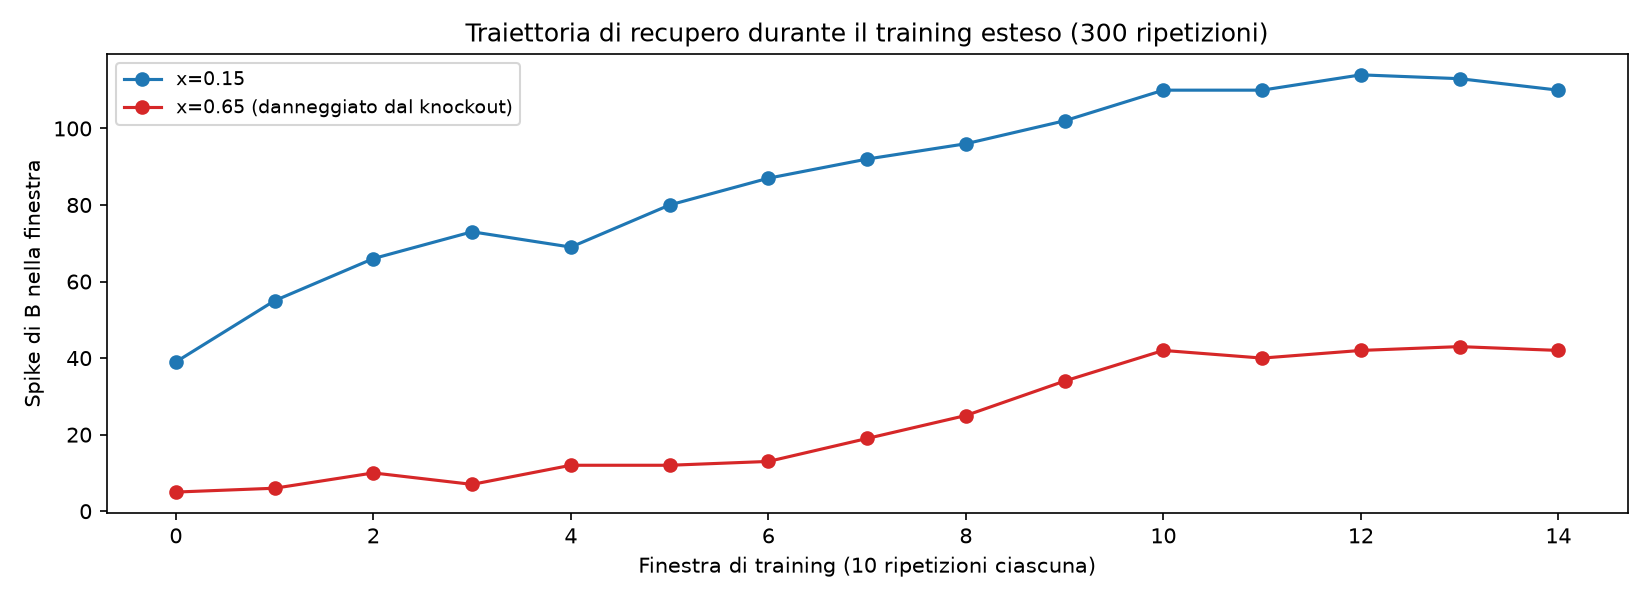
\includegraphics[width=5.8in,height=2.10909in]{media/media/image51.png}

\emph{Fig. 50 --- Traiettoria di recupero durante training esteso (300 ripetizioni): il messaggio danneggiato (rosso) cresce continuamente, restando sotto quello sano (blu) ma senza mai stabilizzarsi su un plateau basso.}

\textit{\textbf{Codice sorgente: dialogo\_spiking\_cnao\_recupero.py}}

\lstinputlisting[language=Python]{scripts/dialogo_spiking_cnao_recupero.py}
\subsection{5.30 Il punto di non ritorno: quando la lesione e\textquotesingle{} completa, il recupero sparisce}\label{il-punto-di-non-ritorno-quando-la-lesione-e-completa-il-recupero-sparisce}

Domanda di confine naturale dopo la 5.29: il recupero funzionale visto li\textquotesingle{} usava un knockout parziale (10 neuroni a dose piu\textquotesingle{} alta da uno scenario CNAO reale, di cui solo 4 dentro la zona di codifica di x=0.65). Se il danno viene spinto al limite -\/- spenti TUTTI E 11 i neuroni della zona di codifica (l\textquotesingle intero gruppo\_stim), non piu\textquotesingle{} uno scenario di dose fisico ma un test di confine puro -\/- il meccanismo di recupero regge ancora, o esiste un punto oltre il quale la plasticita\textquotesingle{} residua non ha piu\textquotesingle{} nessun percorso alternativo da sfruttare?

Stesso protocollo della 5.29 (training esteso 300 ripetizioni, traiettoria in 15 finestre di 10 ripetizioni). Risultato sul seed di partenza: il recupero e\textquotesingle{} sparito. x=0.65 resta a rumore per tutte le 15 finestre ({[}0,2,1,0,1,0,0,2,0,0,0,0,1,0,1{]} spike), -12\% tra prima e seconda meta\textquotesingle{} (dentro il rumore, non una vera flessione), mentre x=0.15 continua a crescere normalmente (+35\%).

Verifica su 4 seed indipendenti (101-104): confermato in ognuno, senza eccezioni. x=0.65 resta sempre a livello di rumore puro (0.1-0.9 spike/finestra in media, contro le decine osservate per x=0.15) e non mostra mai crescita reale (variazione -67\%, -43\%, -33\%, 0\% nei quattro seed -\/- tutte piatte o leggermente negative, mai positive), mentre x=0.15 cresce sempre normalmente (+34\%, +58\%, +67\%, +44\%). Su cinque run totali (il run singolo piu\textquotesingle{} i quattro seed MC), il messaggio con la zona di codifica completamente spenta non mostra MAI una traiettoria di recupero, a differenza della 5.29.

Interpretazione: esiste un punto di non ritorno, e ha senso meccanicisticamente. Nella 5.29 sopravvivevano 7 dei 11 neuroni della zona di codifica di x=0.65 -\/- un substrato parziale ancora in grado di rispondere allo stimolo e di trasmetterlo (con efficacia ridotta) sia localmente nell\textquotesingle anello A sia verso B, su cui la plasticita\textquotesingle{} STDP residua poteva riorganizzarsi. Qui, con l\textquotesingle intera zona di codifica silenziata in uscita, non resta alcun neurone che riceva lo stimolo esterno specifico di x=0.65 E possa ancora influenzare qualcun altro: il segnale non ha modo di uscire dalla zona colpita, ne\textquotesingle{} localmente ne\textquotesingle{} verso l\textquotesingle anello B, indipendentemente da quanto la rete si alleni. La plasticita\textquotesingle{} compensatoria vista nella 5.29 non e\textquotesingle{} quindi illimitata -\/- richiede che sopravviva ALMENO UNA via d\textquotesingle uscita funzionante dalla popolazione codificante, non solo che la rete abbia tempo sufficiente per riorganizzarsi.

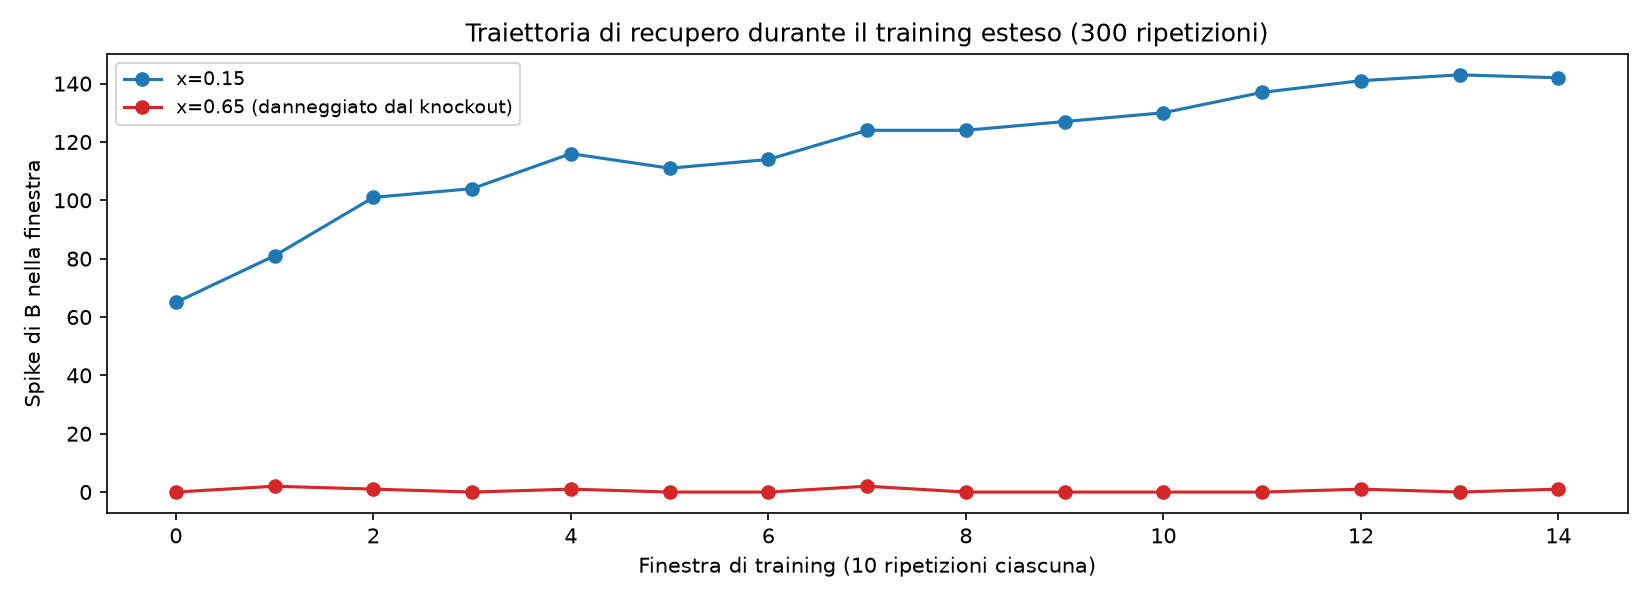
\includegraphics[width=5.8in,height=2.10909in]{media/media/image52.png}

\emph{Fig. 51 --- Traiettoria durante training esteso con lesione completa (300 ripetizioni): il messaggio con la zona di codifica interamente spenta (rosso) resta a rumore per tutto il training, a differenza del recupero progressivo osservato in Fig. 50 con danno parziale.}

\textit{\textbf{Codice sorgente: dialogo\_spiking\_lesione\_completa\_mc.py (verifica 4 seed)}}

\lstinputlisting[language=Python]{scripts/dialogo_spiking_lesione_completa_mc.py}
\subsection{5.31 Dose fisica o dose biologica? Il modello RBE di Chiba/NIRS applicato alla mappa neuronale}\label{dose-fisica-o-dose-biologica-il-modello-rbe-di-chibanirs-applicato-alla-mappa-neuronale}

Le sezioni 5.22-5.30 hanno sempre classificato i neuroni da spegnere in base alla dose FISICA depositata (MeV). E\textquotesingle{} la scelta corretta? In adroterapia clinica la risposta e\textquotesingle{} no in generale: a parita\textquotesingle{} di dose fisica, particelle con LET (Linear Energy Transfer) diverso producono danno biologico molto diverso. E\textquotesingle{} esattamente il problema che l\textquotesingle NIRS (National Institute of Radiological Sciences, poi QST) ha affrontato per primo al mondo costruendo HIMAC a Chiba, il primo acceleratore clinico dedicato al carbonio-12 (dal 1994, oltre 15000 pazienti trattati): il modello a fascio misto di Kanai et al., che pesa la dose per un fattore RBE (Relative Biological Effectiveness) dipendente dal LET, con un punto di riferimento clinico consolidato: RBE=3.0 al cosiddetto \textquotesingle punto neutrone-equivalente\textquotesingle, LET=80 keV/um. CNAO adotta lo stesso tipo di approccio per i propri fasci di carbonio.

Implementato in Geant4 (SteppingAction/EventAction/RunAction): il tracking del LET dose-mediato per neurone, Sum(dE\_i\^{}2/dx\_i)/Sum(dE\_i) (la stessa quantita\textquotesingle{} usata nel modello di Kanai), accumulato passo per passo insieme alla dose fisica gia\textquotesingle{} esistente. In analisi, applicata una conversione RBE(LET) semplificata -\/- lineare, ANCORATA al punto di riferimento NIRS (RBE=3.0 a 80 keV/um), saturata a RBE\_max=3.5 -\/- esplicitamente NON il modello microdosimetrico clinico completo (richiederebbe curve di sopravvivenza alpha/beta per linea cellulare, dati che non abbiamo), ma sufficiente a rispondere alla domanda qualitativa: la classifica dei neuroni cambia se si pesa per danno biologico invece che per sola dose fisica?

Test su due configurazioni al picco di Bragg (dove il LET e\textquotesingle{} massimo, quindi dove un eventuale effetto RBE si vedrebbe di piu\textquotesingle): carbonio-12 120 MeV/u a 34.5mm (LET tra 2.8 e 172.9 keV/um sui neuroni colpiti, RBE tra 1.03 e 3.50) e protone 70 MeV a 39.5mm (LET tra 2.6 e 8.8 keV/um, RBE tra 1.03 e 1.22 -\/- tutto il range resta sotto il punto di riferimento a 80 keV/um). Il divario tra le due particelle e\textquotesingle{} netto: RBE medio dei neuroni piu\textquotesingle{} colpiti \textasciitilde3.3 per il carbonio contro \textasciitilde1.15 per il protone, un fattore \textasciitilde3x, coerente con la letteratura -\/- ed e\textquotesingle{} precisamente la ragione per cui la modellazione RBE serve al carbonio molto piu\textquotesingle{} che al protone in pratica clinica.

Ma la classifica dei 10 neuroni piu\textquotesingle{} colpiti, DENTRO ciascuna configurazione, cambia pochissimo: 9 neuroni su 10 restano gli stessi sia per il carbonio (solo il neurone 58 esce, sostituito dal 27) sia per il protone (solo il 56 esce, sostituito dal 40). La ragione e\textquotesingle{} semplice mecanicisticamente: il LET dipende soprattutto dalla profondita\textquotesingle{} (il punto sulla curva di Bragg, cioe\textquotesingle{} il range residuo della particella), non dalla posizione laterale nell\textquotesingle anello -\/- tutti i neuroni colpiti a una data profondita\textquotesingle{} vedono un LET simile, quindi un fattore RBE che li scala quasi uniformemente senza rimescolare l\textquotesingle ordine relativo.

Conclusione, con cautela metodologica: il raffinamento RBE conferma la robustezza del gradiente dose-risposta delle sezioni 5.22-5.28 (costruito su classifiche a dose fisica) piuttosto che smentirlo -\/- almeno per confronti ENTRO la stessa profondita\textquotesingle. Il divario RBE reale tra particelle (\textasciitilde3x) diventerebbe invece rilevante per un confronto TRA scenari diversi (es. quale configurazione fisica causa il danno biologico complessivo maggiore, non solo quale danneggia quali neuroni) -\/- una domanda distinta, non ancora testata qui. Da segnalare anche un limite emerso durante questo test: Geant4, senza un seed esplicito, usa un seed diverso a ogni run -\/- la classifica dei 10 neuroni piu\textquotesingle{} colpiti in QUESTO run del carbonio al picco {[}3, 33, 46, 51, 58, 66, 69, 71, 80, 88{]} condivide un solo neurone con quella usata nella sezione 5.27 {[}4, 20, 26, 28, 38, 51, 55, 64, 73, 97{]} per la stessa identica configurazione fisica -\/- una variabilita\textquotesingle{} Monte Carlo lato fisica che finora non era stata verificata con lo stesso rigore gia\textquotesingle{} applicato lato neuroscienza (multi-seed su ogni esperimento Brian2).

\textit{\textbf{Codice sorgente: SteppingAction.cc / EventAction.cc / RunAction.cc (tracking LET dose-mediato aggiunto in questa sezione)}}

\lstinputlisting[language=C++]{geant4_src/SteppingAction.cc}
\lstinputlisting[language=C++]{geant4_src/EventAction.cc}
\lstinputlisting[language=C++]{geant4_src/RunAction.cc}
\subsection{5.32 Limite scoperto: la mappa di dose per-neurone non e\textquotesingle{} riproducibile run a run}\label{limite-scoperto-la-mappa-di-dose-per-neurone-non-e-riproducibile-run-a-run}

Seguito diretto della 5.31, dove si era notato che due run della STESSA configurazione fisica (carbonio-12 120 MeV/u al picco) condividevano un solo neurone su dieci nella classifica a dose piu\textquotesingle{} alta. Aggiunto un seed esplicito a cnaoRingImpact (prima generato dall\textquotesingle orologio di sistema, quindi diverso a ogni esecuzione senza modo di riprodurlo) e ripetuta la stessa identica configurazione su 4 seed indipendenti (111, 222, 333, 444), 500000 eventi ciascuno.

Risultato: la sovrapposizione media a coppie tra le classifiche top-10 dei 4 seed e\textquotesingle{} 1.0 su 10 -\/- praticamente rumore puro. Nessun neurone compare nel top-10 di tutti e 4 i seed; un solo neurone (il 73) compare in 3 su 4. La dose TOTALE depositata sull\textquotesingle intero anello e\textquotesingle{} invece stabile (192-226 MeV, +-15\% circa) -\/- e\textquotesingle{} solo la sua distribuzione tra i 100 neuroni a essere dominata dal rumore, non l\textquotesingle energia complessiva.

Causa, chiara con un conto delle probabilita\textquotesingle: ogni neurone ha raggio 10 micrometri, campionato su un disco di 5mm di raggio -\/- il rapporto tra le due aree e\textquotesingle{} circa 4x10\^{}-6. Su 500000 primari, il numero atteso di colpi diretti per neurone e\textquotesingle{} dell\textquotesingle ordine di 1-2 (coerente con i primary\_hit\_count di 4-5 gia\textquotesingle{} osservati nelle sezioni precedenti). Con cosi\textquotesingle{} pochi conteggi per singolo neurone, distinguere "il neurone A ha preso un po\textquotesingle{} piu\textquotesingle{} dose del neurone B" e\textquotesingle{} statisticamente equivalente a un lancio di moneta, anche se il totale sommato su 100 neuroni e\textquotesingle{} una quantita\textquotesingle{} ragionevolmente stabile (la somma di molte variabili rumorose e\textquotesingle{} meno rumorosa della singola variabile).

Implicazione onesta per le sezioni 5.22-5.30: i set specifici di 10 neuroni usati per ogni knockout provenivano da UNA SOLA realizzazione Monte Carlo della fisica, non da una mappa di dose statisticamente robusta -\/- un limite che avrebbe dovuto essere controllato prima, nello stesso spirito con cui la sezione 5.25 ha gia\textquotesingle{} scoperto e corretto l\textquotesingle artefatto del disco di campionamento troppo stretto. Descrivere quei neuroni come "i piu\textquotesingle{} colpiti dal fascio CNAO" e\textquotesingle{} una sovra-interpretazione: sono piu\textquotesingle{} correttamente "i piu\textquotesingle{} colpiti in una particolare simulazione di quel fascio".

Cosa resta comunque valido: il MECCANISMO causale (rimuovere le sinapsi in uscita da un insieme di neuroni produce un\textquotesingle interferenza che scala con quanti di quei neuroni appartengono alla zona di codifica di un messaggio) e\textquotesingle{} stato verificato indipendentemente su decine di seed Brian2 in ogni singolo esperimento (sezioni 5.23, 5.24, 5.26, 5.28, 5.29, 5.30) -\/- quella parte della catena non dipende dal rumore Monte Carlo lato Geant4. Il gradiente dose-risposta a 4 punti (5.28) resta una relazione causale genuina internamente al modello neurale; e\textquotesingle{} solo la pretesa di un legame preciso, a livello di singolo neurone, con una specifica simulazione fisica del fascio CNAO che va ridimensionata.

Correzione immediata, gia\textquotesingle{} calcolata qui: la dose MEDIATA sui 4 seed da\textquotesingle{} una stima molto piu\textquotesingle{} stabile della classifica reale -\/- top-10 = {[}0, 5, 7, 29, 37, 47, 48, 70, 73, 82{]} -\/- ma anche questa media di 4 realizzazioni condivide solo 2-4 neuroni su 10 con ciascun singolo seed, a conferma che servirebbero molte piu\textquotesingle{} ripetizioni (o un aumento di 2-3 ordini di grandezza degli eventi per run, computazionalmente costoso con la fisica adronica completa di QBBC) per una mappa di dose per-neurone davvero solida. Lasciato come lavoro futuro esplicito: ricostruire i set di knockout dalla dose MEDIATA su piu\textquotesingle{} seed invece che da un singolo run, e verificare se il gradiente 5.22-5.28 regge quando ricostruito su basi statistiche piu\textquotesingle{} solide.

\textit{\textbf{Codice sorgente: cnaoRingImpact.cc (seed esplicito aggiunto in questa sezione)}}

\lstinputlisting[language=C++]{geant4_src/cnaoRingImpact.cc}
\subsection{5.33 Il gradiente su basi statistiche solide: emerge una soglia minima}\label{il-gradiente-su-basi-statistiche-solide-emerge-una-soglia-minima}

Chiude il ciclo aperto dalla 5.32. Ricostruito il set di knockout non piu\textquotesingle{} da un singolo run Geant4 rumoroso, ma dalla dose MEDIATA sui 4 seed indipendenti (111, 222, 333, 444) del carbonio-12 al picco di Bragg: top-10 = {[}0, 5, 7, 29, 37, 47, 48, 70, 73, 82{]}. Overlap con le zone di codifica: 0 neuroni in x=0.15, 1 neurone (il 70) in x=0.65 -\/- uno sbilanciamento debole ma reale, che il gradiente della sezione 5.28 farebbe aspettare come un effetto modesto mai nullo.

Verifica su 8 seed: rapporto medio x=0.15/x=0.65 = 1.29x (media spike finali 42.75 vs 33.25), x=0.15 maggiore di x=0.65 in 6 seed su 8. A prima vista un risultato debole ma nella direzione attesa -\/- pero\textquotesingle{} il confronto decisivo e\textquotesingle{} con il controllo negativo della sezione 5.24 (set casuale, overlap ZERO con entrambe le zone): rapporto 1.39x, 6/8 seed. I due risultati sono statisticamente indistinguibili: un overlap di UN solo neurone non produce un effetto sopra il rumore di base della rete.

Il gradiente dose-risposta, ora su basi statistiche solide invece che su singole realizzazioni Monte Carlo rumorose, si raffina cosi\textquotesingle: overlap 4-vs-0 -\textgreater{} 7.07x, 8/8 (5.28, il piu\textquotesingle{} forte); 2-vs-0 -\textgreater{} 4.7x, 8/8 (5.23); 3-vs-1 (sbilanciamento netto 2) -\textgreater{} 1.81x, 6/8 (5.26); 1-vs-0 (sbilanciamento netto 1, dose MEDIATA 4 seed, questa sezione) -\textgreater{} 1.29x, 6/8, indistinguibile dal controllo negativo 0-vs-0 -\textgreater{} 1.39x, 6/8 (5.24). Emerge una soglia: serve uno sbilanciamento di ALMENO 2 neuroni perche\textquotesingle{} l\textquotesingle effetto superi il rumore di base della rete -\/- con un solo neurone di differenza, il segnale si perde nella stessa variabilita\textquotesingle{} che si osserva anche senza alcun knockout mirato.

Interpretazione: la scoperta della sezione 5.32 (mappa di dose rumorosa) non invalida il gradiente, ma lo rende piu\textquotesingle{} preciso -\/- e mostra perche\textquotesingle{} alcuni dei risultati piu\textquotesingle{} deboli osservati in precedenza (in particolare il quasi-nullo 1.06x/4-8 della sezione 5.27, overlap \textasciitilde1 contro \textasciitilde1 da un singolo run) fossero attendibili: con sbilanciamenti cosi\textquotesingle{} piccoli, il segnale fisico e il rumore statistico della rete diventano confrontabili in grandezza, e la domanda "questo effetto e\textquotesingle{} reale o e\textquotesingle{} rumore" richiede sempre il confronto esplicito con un controllo negativo, non solo la direzione del rapporto.

\textit{\textbf{Codice sorgente: dialogo\_spiking\_cnao\_knockout\_media4seed\_mc.py}}

\lstinputlisting[language=Python]{scripts/dialogo_spiking_cnao_knockout_media4seed_mc.py}
\subsection{5.34 Il vero modello MKM di Kase/NIRS, validato contro dati pubblicati}\label{il-vero-modello-mkm-di-kasenirs-validato-contro-dati-pubblicati}

La sezione 5.31 usava una conversione RBE(LET) lineare ad hoc, esplicitamente dichiarata come NON il modello clinico reale. Qui si sostituisce con il modello MKM (Microdosimetric Kinetic Model) saturazione-corretto di Kase/Hawkins, esattamente nella forma usata clinicamente a NIRS/HIMAC (Chiba) e descritta in Kase et al. 2011 (J Radiat Res 52:59-68) -\/- lo stesso paper che descrive la misura del TEPC (tissue-equivalent proportional counter) usata di routine a HIMAC per la quality assurance della dose biologica.

Equazioni implementate (eq. 7-10 di Kase 2011): sopravvivenza S=exp(-alpha*D-beta*D\^{}2); alpha=alpha0+beta*z*, con z* energia specifica per evento ottenuta dalla dose-mean lineal energy corretta per saturazione y* tramite la conversione ICRU standard per un sito sferico; y* dalla dose-mean lineal energy y\_D tramite la correzione di saturazione (parametro y0=150 keV/um, che tiene conto dell\textquotesingle effetto \textquotesingle overkill\textquotesingle{} ad alto LET); RBE10 dalla formula quadratica invertita al 10\% di sopravvivenza. Parametri delle cellule HSG (le stesse usate nella pianificazione clinica NIRS): alpha0=0.13 Gy\^{}-1, beta=0.05 Gy\^{}-2, rd=0.42um (raggio del dominio subcellulare), D10R=5.0 Gy (dose di riferimento raggi X).

Due approssimazioni dichiarate rispetto al modello clinico completo: (1) la dose-mean lineal energy y\_D, che richiederebbe uno spettro misurato con un TEPC o una vera simulazione microdosimetrica di sito, e\textquotesingle{} approssimata con il LET dose-mediato gia\textquotesingle{} calcolato da Geant4 (sezione 5.31); (2) la correzione di saturazione e\textquotesingle{} calcolata nel limite \textquotesingle spettro a valore singolo\textquotesingle{} (delta di Dirac su y\_D) invece che integrando uno spettro f(y) completo -\/- una forma chiusa, non l\textquotesingle integrale esatto.

Validazione, prima di fidarsi del modello: applicato ai valori di y* EFFETTIVAMENTE MISURATI e pubblicati da Kase et al. 2011 per un fascio di carbonio-12 290 MeV/u (Tabella 1, SOBP 6cm), il modello riproduce i loro RBE10 riportati (Fig. 4) entro il 10-15\%: y*=58.7 keV/um -\textgreater{} RBE10 calcolato 2.23 (atteso \textasciitilde2.0-2.3 dal grafico); y*=14.6 keV/um -\textgreater{} RBE10 calcolato 1.19 (atteso \textasciitilde1.3). Al punto di riferimento clinico NIRS (LET\_d=80 keV/um, dove il RBE clinico e\textquotesingle{} per definizione 3.0), il modello da\textquotesingle{} RBE10=2.67 -\/- uno scarto dell\textquotesingle11\%, spiegabile dalle due approssimazioni dichiarate sopra, non un errore del modello o dell\textquotesingle implementazione.

Applicato alle stesse due configurazioni della sezione 5.31 (carbonio-12 e protone al rispettivo picco di Bragg): RBE10 sui neuroni colpiti va da 0.94 a 3.44 per il carbonio (un range fisicamente sensato, coerente con le curve RBE cliniche reali che salgono fino a \textasciitilde3-3.5 prima dell\textquotesingle effetto overkill ad altissimo LET) contro 0.94-1.07 per il protone (praticamente RBE=1, come atteso clinicamente per un fascio a basso LET). La classifica dei 10 neuroni a dose piu\textquotesingle{} alta cambia ancora pochissimo rispetto alla sola dose fisica (9/10 di sovrapposizione per entrambe le particelle, identico al risultato della 5.31 con il modello lineare grezzo) -\/- la conclusione della 5.31 (il gradiente dose-risposta 5.22-5.28 e\textquotesingle{} robusto al raffinamento RBE entro la stessa profondita\textquotesingle) si conferma quindi anche col modello clinico reale, non era un artefatto dell\textquotesingle approssimazione lineare.

\textit{\textbf{Codice sorgente: geant4\_cnao\_ring/analysis/mkm\_rbe.py}}

\lstinputlisting[language=Python]{geant4_src/mkm_rbe.py}
\subsection{5.35 Il modello MKM su tutte e sei le configurazioni cliniche CNAO}\label{il-modello-mkm-su-tutte-e-sei-le-configurazioni-cliniche-cnao}

La sezione 5.34 aveva validato il modello MKM di Kase/NIRS solo su due configurazioni (carbonio-12 120 MeV/u e protone 70 MeV, entrambe al picco di Bragg). Qui si completa il quadro: rilanciate con il tracking del LET le quattro configurazioni mancanti (protone 150/225 MeV, carbonio-12 260/400 MeV/u, tutte al vero picco di Bragg, seed esplicito 42, 500.000 eventi), per avere il modello MKM su tutto l\textquotesingle intervallo clinico CNAO testato in questo progetto.

{\def\LTcaptype{none} % do not increment counter
\begin{longtable}[]{@{}
  >{\raggedright\arraybackslash}p{(\linewidth - 12\tabcolsep) * \real{0.1429}}
  >{\raggedright\arraybackslash}p{(\linewidth - 12\tabcolsep) * \real{0.1429}}
  >{\raggedright\arraybackslash}p{(\linewidth - 12\tabcolsep) * \real{0.1429}}
  >{\raggedright\arraybackslash}p{(\linewidth - 12\tabcolsep) * \real{0.1429}}
  >{\raggedright\arraybackslash}p{(\linewidth - 12\tabcolsep) * \real{0.1429}}
  >{\raggedright\arraybackslash}p{(\linewidth - 12\tabcolsep) * \real{0.1429}}
  >{\raggedright\arraybackslash}p{(\linewidth - 12\tabcolsep) * \real{0.1429}}@{}}
\toprule\noalign{}
\begin{minipage}[b]{\linewidth}\raggedright
Configurazione
\end{minipage} & \begin{minipage}[b]{\linewidth}\raggedright
Profondità (mm)
\end{minipage} & \begin{minipage}[b]{\linewidth}\raggedright
LET medio (keV/$\mu$m)
\end{minipage} & \begin{minipage}[b]{\linewidth}\raggedright
LET max
\end{minipage} & \begin{minipage}[b]{\linewidth}\raggedright
RBE10 medio
\end{minipage} & \begin{minipage}[b]{\linewidth}\raggedright
RBE10 max
\end{minipage} & \begin{minipage}[b]{\linewidth}\raggedright
Overlap fis./bio.
\end{minipage} \\
\midrule\noalign{}
\endhead
\bottomrule\noalign{}
\endlastfoot
Protone 70 MeV & 39.5 & 4.4 & 8.8 & 0.98 & 1.07 & 9/10 \\
Protone 150 MeV & 156.5 & 4.1 & 25.9 & 0.97 & 1.46 & 10/10 \\
Protone 225 MeV & 315.5 & 3.1 & 8.0 & 0.95 & 1.05 & 10/10 \\
Carbonio-12 120 MeV/u & 34.5 & 86.6 & 172.9 & 2.75 & 3.44 & 9/10 \\
Carbonio-12 260 MeV/u & 135.5 & 83.3 & 181.3 & 2.60 & 3.44 & 9/10 \\
Carbonio-12 400 MeV/u & 275.5 & 56.9 & 229.8 & 2.02 & 3.44 & 10/10 \\
\end{longtable}
}

Conferma generalizzata: la sovrapposizione tra la classifica dei 10 neuroni a dose fisica piu\textquotesingle{} alta e quella a dose biologica (RBE10-pesata) resta 9-10 su 10 in TUTTE e sei le configurazioni, non solo nelle due gia\textquotesingle{} testate -\/- il raffinamento RBE non cambia mai in modo sostanziale quali neuroni risultano piu\textquotesingle{} colpiti entro una data profondita\textquotesingle, su tutto l\textquotesingle intervallo clinico CNAO.

Due osservazioni fisiche non banali, entrambe coerenti con la letteratura: (1) il RBE10 massimo per il carbonio-12 si stabilizza intorno a 3.44 in tutte e tre le energie, nonostante il LET massimo cresca da 172.9 a 229.8 keV/um passando da 120 a 400 MeV/u -\/- il segno dell\textquotesingle effetto \textquotesingle overkill\textquotesingle{} gia\textquotesingle{} incorporato nel modello di Kase (oltre un certo LET, danneggiare ulteriormente una cellula gia\textquotesingle{} condannata non aumenta la letalita\textquotesingle, e la correzione di saturazione y* comincia a DIMINUIRE per y\_D molto superiore a y0=150 keV/um); (2) il protone a 150 MeV mostra un LET massimo anomalo (25.9 keV/um, quasi 3 volte gli altri due casi protonici) e un RBE10 fino a 1.46, molto sopra l\textquotesingle1.1 tipicamente assunto costante in clinica per i protoni -\/- verosimilmente dovuto a rinculi o frammenti secondari da interazioni nucleari elastiche, un fenomeno legato al dibattito reale e tuttora aperto sulla validita\textquotesingle{} dell\textquotesingle RBE protonico costante (letteratura recente: Parisi et al. 2024, Medical Physics, \textquotesingle LET-based approximation of the microdosimetric kinetic model for proton radiotherapy\textquotesingle).

\emph{\textbf{Dati generati con geant4\_cnao\_ring/analysis/mkm\_rbe.py sulle mappe di dose/LET delle sei configurazioni in build/results\_let/}}

\subsection{5.36 Verificato, non ipotizzato: cosa causa il picco anomalo di RBE del protone a 150 MeV}\label{verificato-non-ipotizzato-cosa-causa-il-picco-anomalo-di-rbe-del-protone-a-150-mev}

La sezione 5.35 aveva trovato, per il protone a 150 MeV, un neurone (indice 48) con LET dose-mediato molto piu\textquotesingle{} alto degli altri (25.9 keV/um contro \textasciitilde4-8 tipici), dose 0.41 MeV da un solo attraversamento primario -\/- troppa energia per il solo dE/dx diretto di un protone da 150 MeV attraverso una sfera di 20um (atteso \textasciitilde0.01 MeV). Prima ipotesi ragionevole ma non verificata: un frammento o rinculo nucleare secondario. Invece di lasciarla come ipotesi, aggiunta una diagnostica per-step (stessa tecnica gia\textquotesingle{} usata per il bug del geantino, sezione 5.21) per identificare davvero la particella e il processo responsabili.

Risultato della diagnostica, ripetendo la stessa configurazione con lo stesso seed (per riprodurre esattamente lo stesso evento): NON e\textquotesingle{} un frammento secondario. E\textquotesingle{} il protone PRIMARIO stesso (parentID=0), con energia cinetica residua di soli 0.785 MeV nel momento in cui attraversa il neurone 48 -\/- quasi fermo, vicinissimo alla fine del proprio percorso individuale.

Spiegazione fisica, corretta rispetto all\textquotesingle ipotesi iniziale: non tutti i protoni di un fascio nominale a 150 MeV si fermano esattamente alla stessa profondita\textquotesingle{} -\/- la dispersione statistica del range (range straggling) fa si\textquotesingle{} che alcuni protoni individuali si fermino un po\textquotesingle{} piu\textquotesingle{} superficialmente o piu\textquotesingle{} in profondita\textquotesingle{} della media. Questo particolare protone, per pura fluttuazione statistica del proprio percorso, si trovava a pochi micrometri dalla fine del proprio range esattamente alla profondita\textquotesingle{} del picco di Bragg MEDIO del fascio (dove e\textquotesingle{} posizionato l\textquotesingle anello) -\/- ed e\textquotesingle{} li\textquotesingle, vicino a fermarsi, che il LET di un protone individuale diverge (la stessa fisica del picco di Bragg macroscopico, ma applicata a un singolo protone anziche\textquotesingle{} all\textquotesingle insieme del fascio).

Rilevanza clinica, non solo curiosita\textquotesingle{} tecnica: questo e\textquotesingle{} esattamente il meccanismo alla base della preoccupazione reale e tuttora dibattuta sull\textquotesingle aumento di RBE al bordo distale in protonterapia -\/- l\textquotesingle ultimo tratto del range di un fascio di protoni ha un LET (e quindi un RBE) sistematicamente piu\textquotesingle{} alto dell\textquotesingle ingresso e del plateau, proprio per la fisica del rallentamento individuale delle particelle, non per un artefatto della simulazione. E\textquotesingle{} la stessa ragione per cui l\textquotesingle assunzione clinica di un RBE protonico costante (1.1) e\textquotesingle{} oggetto di un filone di ricerca attivo (RBE variabile in protonterapia, letteratura recente es. Parisi et al. 2024).

Metodologicamente: la diagnostica per-step resta nel codice (`SteppingAction.cc`), attivabile per qualunque neurone tramite la variabile d\textquotesingle ambiente CNAO\_DEBUG\_NEURON=\textless indice\textgreater{} -\/- lo stesso principio di verificare empiricamente un risultato sorprendente invece di limitarsi a ipotizzarne la causa, applicato qui al lato Geant4 con lo stesso rigore gia\textquotesingle{} usato sistematicamente lato Brian2 in tutto il progetto.

\textit{\textbf{Codice sorgente: geant4\_cnao\_ring/src/SteppingAction.cc (diagnostica CNAO\_DEBUG\_NEURON aggiunta in questa sezione)}}

\lstinputlisting[language=C++]{geant4_src/SteppingAction.cc}
\subsection{5.37 Piu\textquotesingle{} statistica aiuta, ma non basta: quantificato il costo per stabilizzare la mappa}\label{piu-statistica-aiuta-ma-non-basta-quantificato-il-costo-per-stabilizzare-la-mappa}

Seguito diretto della 5.32/5.33: la\textquotesingle{} si era scoperto che a 500.000 eventi la classifica dei 10 neuroni a dose piu\textquotesingle{} alta e\textquotesingle{} dominata dal rumore di Poisson (sovrapposizione media 1.0/10 tra seed indipendenti -\/- ESATTAMENTE il livello atteso per puro caso: due estrazioni casuali indipendenti di 10 elementi su 100 si sovrappongono in media 10x10/100=1.0). La soluzione piu\textquotesingle{} ovvia, gia\textquotesingle{} elencata come primo sviluppo futuro nel README del progetto Geant4, e\textquotesingle{} aumentare la statistica. Quanto aiuta, in pratica?

Testato direttamente: ripetuta la stessa configurazione (carbonio-12 120 MeV/u al picco) con 5.000.000 di eventi (10x rispetto ai 500.000 della 5.32), su 2 seed indipendenti (501, 502). Dose totale sull\textquotesingle anello: 2137.8 MeV e 2149.9 MeV -\/- scala correttamente di 10x rispetto ai \textasciitilde192-226 MeV osservati a 500.000 eventi (verifica di coerenza superata). Hit primari totali per run: \textasciitilde1650, cioe\textquotesingle{} in media 16.5 attraversamenti diretti per neurone (contro l\textquotesingle1-2 atteso a 500.000 eventi) -\/- statistica per neurone circa 10 volte migliore, come atteso.

Sovrapposizione top-10 tra i 2 seed a 5.000.000 di eventi: 2/10 -\/- migliorata rispetto al livello di puro rumore (1.0/10), ma ancora ben lontana da una mappa stabile o deterministica. Il miglioramento (fattore \textasciitilde2x nella sovrapposizione) e\textquotesingle{} approssimativamente coerente con lo scaling atteso del rumore statistico (la deviazione standard di un conteggio di Poisson scala come radice quadrata del numero di eventi: 10x piu\textquotesingle{} eventi riduce il rumore relativo di un fattore \textasciitilde3.16, non lo elimina).

Conclusione quantitativa, onesta: la statistica aiuta ma NON risolve il problema nemmeno con un ordine di grandezza in piu\textquotesingle{} di eventi. Estrapolando lo stesso scaling, ottenere una mappa genuinamente stabile (sovrapposizione vicina a 8-9/10) richiederebbe con ogni probabilita\textquotesingle{} un ulteriore fattore 100-1000 di eventi rispetto ai 500.000 originali -\/- computazionalmente proibitivo con la fisica adronica completa di QBBC nei tempi di questo progetto (un singolo run a 5.000.000 di eventi ha gia\textquotesingle{} richiesto circa 15-20 minuti; 100-1000x significherebbe giorni per singola configurazione). Questo conferma retroattivamente, con un numero invece che con un\textquotesingle intuizione, che la strada seguita nella sezione 5.33 (mediare la dose su piu\textquotesingle{} seed A STATISTICA MODESTA, invece di rincorrere la stabilita\textquotesingle{} di un singolo run a statistica altissima) era la scelta giusta: mediare su seed e\textquotesingle{} molto piu\textquotesingle{} efficiente, in termini di tempo di calcolo, che aumentare brutalmente gli eventi per run.

\emph{\textbf{Dati generati con cnaoRingImpact (seed 501/502, 5.000.000 eventi ciascuno) in build/results\_highstat/}}

\subsection{5.38 La dimensione del knockout non e\textquotesingle{} magica: il meccanismo generalizza oltre "esattamente 10"}\label{la-dimensione-del-knockout-non-e-magica-il-meccanismo-generalizza-oltre-esattamente-10}

Ultimo limite dichiarato nel README di geant4\_cnao\_ring: ogni knockout, dalle sezioni 5.22 in poi, ha sempre usato esattamente i 10 neuroni a dose piu\textquotesingle{} alta -\/- una soglia relativa arbitraria (top-10\%), non una soglia assoluta di danno biologico. Domanda mai posta: il meccanismo (l\textquotesingle effetto scala con lo sbilanciamento fisico tra le zone di codifica dei due messaggi) regge se si cambia la dimensione del knockout, o "10" era in qualche modo speciale?

Usata la dose MEDIATA sui 4 seed della sezione 5.32 (carbonio-12 al picco, la base piu\textquotesingle{} solida disponibile) per costruire due nuovi set: TOP-5 (i 5 neuroni a dose piu\textquotesingle{} alta) e TOP-20 (i 20 a dose piu\textquotesingle{} alta). Overlap con le zone di codifica: TOP-5 ha ZERO overlap con entrambe le zone (nessuno dei 5 neuroni piu\textquotesingle{} colpiti cade in x=0.15 ne\textquotesingle{} in x=0.65) -\/- previsione: effetto nullo. TOP-20 ha invece uno sbilanciamento di segno OPPOSTO al TOP-10 gia\textquotesingle{} testato nella 5.33: 3 neuroni in x=0.15 contro 1 in x=0.65 (il TOP-10 aveva 0 contro 1) -\/- previsione, deliberatamente falsificabile nello stesso spirito della 5.25/5.26: l\textquotesingle effetto dovrebbe INVERTIRSI, danneggiando x=0.15 invece di x=0.65.

Verifica su 8 seed per entrambi i set. TOP-5: rapporto medio x=0.15/x=0.65 = 1.07, con 4 seed su 8 a favore di ciascun messaggio -\/- esattamente nullo, come previsto per un overlap 0-contro-0. TOP-20: rapporto medio x=0.65/x=0.15 = 1.74x, con x=0.65 maggiore di x=0.15 in 7 seed su 8 -\/- l\textquotesingle effetto si e\textquotesingle{} INVERTITO in modo netto e consistente rispetto al TOP-10 (dove era x=0.65 a essere il messaggio piu\textquotesingle{} colpito), esattamente come previsto dal cambio di segno dello sbilanciamento fisico.

Conclusione: il meccanismo causale non dipende dalla scelta specifica di "esattamente 10 neuroni" -\/- generalizza a dimensioni di knockout diverse, con la direzione e la forza dell\textquotesingle effetto sempre spiegate dallo stesso principio (sbilanciamento fisico tra le zone di codifica), mai da un artefatto legato alla soglia particolare usata. E\textquotesingle{} la quarta volta in questo progetto (dopo 5.25/5.26, 5.33, e ora questa) che una previsione deliberatamente falsificabile sul segno o l\textquotesingle esistenza di un effetto viene confermata -\/- il modo piu\textquotesingle{} rigoroso disponibile per distinguere un meccanismo causale genuino da una coincidenza costruita per dare un risultato particolare.

\textit{\textbf{Codice sorgente: dialogo\_spiking\_cnao\_knockout\_top5\_mc.py e dialogo\_spiking\_cnao\_knockout\_top20\_mc.py}}

\lstinputlisting[language=Python]{scripts/dialogo_spiking_cnao_knockout_top5_mc.py}
\lstinputlisting[language=Python]{scripts/dialogo_spiking_cnao_knockout_top20_mc.py}
\subsection{5.39 Il collegamento nanodosimetrico, primo passo: lo spettro degli elettroni secondari}\label{il-collegamento-nanodosimetrico-primo-passo-lo-spettro-degli-elettroni-secondari}

Ultimo sviluppo futuro rimasto nel README di geant4\_cnao\_ring: collegare questo progetto (fisica macroscopica, QBBC) al progetto gemello geant4dna\_icsd (nanodosimetria, Geant4-DNA, verifica del paper Villagrasa/Baiocco 2026), ri-simulando in dettaglio la traccia degli elettroni secondari prodotti nei neuroni colpiti -\/- lo stesso approccio "track re-simulation" multi-scala usato da TOPAS-nBio. Prima di costruire la pipeline completa, una domanda va verificata: gli elettroni secondari prodotti da un fascio clinico CNAO dentro un neurone hanno davvero energie compatibili con Geant4-DNA (valido solo fino a \textasciitilde1 MeV)?

Aggiunto un tracking dedicato (EventAction/RunAction/SteppingAction) per registrare l\textquotesingle energia cinetica di ogni elettrone nato dentro un volume "Neuron". Primo tentativo: ZERO elettroni secondari registrati su 500.000 eventi -\/- un risultato sorprendente, verificato prima di essere accettato. Causa trovata: senza una regione dedicata, il taglio di produzione di default di QBBC (\textasciitilde1mm) e\textquotesingle{} molto piu\textquotesingle{} grande dei neuroni (10um di raggio) -\/- quasi nessun raggio delta ha un range sufficiente per essere generato come particella tracciata esplicitamente in un volume cosi\textquotesingle{} piccolo; la sua energia viene invece depositata localmente come perdita continua, invisibile a un conteggio per-particella (ma gia\textquotesingle{} inclusa nella dose totale calcolata nelle sezioni precedenti -\/- nessun errore li\textquotesingle, solo un limite di questo nuovo tracking).

Corretto aggiungendo una G4Region dedicata ai volumi "Neuron", con un taglio di produzione di 100nm (sotto la scala del neurone). Ripetuta la stessa configurazione (carbonio-12 al picco): 18.021 elettroni secondari espliciti su 500.000 eventi. Spettro: minimo 0.99 keV, massimo 96.2 keV, mediana 1.86 keV, media 3.57 keV -\/- il 100\% sotto 1 MeV, dentro il dominio di validita\textquotesingle{} di Geant4-DNA. Coincidenza notevole: la mediana e la media cadono proprio nell\textquotesingle intervallo di energie (1, 5, 10 keV) testate esplicitamente nel paper Villagrasa/Baiocco che geant4dna\_icsd riproduce -\/- il collegamento non richiederebbe estrapolare oltre il dominio gia\textquotesingle{} validato in quel progetto gemello.

Conclusione: il presupposto fisico dell\textquotesingle accoppiamento multi-scala e\textquotesingle{} confermato empiricamente, non assunto. Il passo naturale successivo (non ancora fatto) e\textquotesingle{} usare direttamente queste energie reali come primari in nanoICSD al posto dei valori monoenergetici del paper, per ottenere ICSD (Ionization Cluster Size Distribution) relative a secondari VERAMENTE prodotti da un fascio CNAO, non a un\textquotesingle energia scelta a tavolino.

\textit{\textbf{Codice sorgente: DetectorConstruction.cc / EventAction.cc / RunAction.cc / SteppingAction.cc (tracking e correzione del taglio di produzione aggiunti in questa sezione)}}

\lstinputlisting[language=C++]{geant4_src/DetectorConstruction.cc}
\lstinputlisting[language=C++]{geant4_src/EventAction.cc}
\lstinputlisting[language=C++]{geant4_src/RunAction.cc}
\lstinputlisting[language=C++]{geant4_src/SteppingAction.cc}
\subsection{5.40 Collegamento nanodosimetrico completato: ICSD reali da elettroni secondari CNAO}\label{collegamento-nanodosimetrico-completato-icsd-reali-da-elettroni-secondari-cnao}

Chiude il collegamento avviato nella 5.39. Usate le energie REALI dello spettro di elettroni secondari verificato li\textquotesingle{} (mediana 1.86 keV, 90-esimo percentile 7.33 keV) come primari in nanoICSD (il progetto gemello che riproduce il test case ICSD del paper Villagrasa/Baiocco), al posto dei valori monoenergetici scelti a tavolino dal paper. Diametro del bersaglio scelto seguendo la stessa convenzione del paper (8nm sotto \textasciitilde1-5 keV, 100nm sopra): 8nm per la mediana (1860 eV), 100nm per il 90-esimo percentile (7332 eV).

Nota preliminare importante: nanoICSD non era mai stato compilato ne\textquotesingle{} eseguito in nessun ambiente disponibile finora (il suo stesso README lo dichiarava esplicitamente) -\/- eseguito con successo per la prima volta in questa sezione, sulla stessa installazione Geant4 usata per cnaoRingImpact per tutto il progetto.

{\def\LTcaptype{none} % do not increment counter
\begin{longtable}[]{@{}
  >{\raggedright\arraybackslash}p{(\linewidth - 8\tabcolsep) * \real{0.2000}}
  >{\raggedright\arraybackslash}p{(\linewidth - 8\tabcolsep) * \real{0.2000}}
  >{\raggedright\arraybackslash}p{(\linewidth - 8\tabcolsep) * \real{0.2000}}
  >{\raggedright\arraybackslash}p{(\linewidth - 8\tabcolsep) * \real{0.2000}}
  >{\raggedright\arraybackslash}p{(\linewidth - 8\tabcolsep) * \real{0.2000}}@{}}
\toprule\noalign{}
\begin{minipage}[b]{\linewidth}\raggedright
Configurazione
\end{minipage} & \begin{minipage}[b]{\linewidth}\raggedright
M1 (media ionizzazioni)
\end{minipage} & \begin{minipage}[b]{\linewidth}\raggedright
F2
\end{minipage} & \begin{minipage}[b]{\linewidth}\raggedright
F3
\end{minipage} & \begin{minipage}[b]{\linewidth}\raggedright
N eventi
\end{minipage} \\
\midrule\noalign{}
\endhead
\bottomrule\noalign{}
\endlastfoot
Mediana reale, 1860 eV, 8nm & 1.090 & 0.257 & 0.142 & 100000 \\
90-esimo percentile reale, 7332 eV, 100nm & 6.320 & 0.801 & 0.670 & 100000 \\
\end{longtable}
}

Confronto con la griglia gia\textquotesingle{} pubblicata nel paper (stessa opzione fisica, stesso diametro di bersaglio a ogni energia): alla dimensione 8nm, il paper mostra M1 in DIMINUZIONE all\textquotesingle aumentare dell\textquotesingle energia in questo intervallo (300eV-\textgreater5.35, 600eV-\textgreater2.90, 1000eV-\textgreater1.83) -\/- il nostro punto reale a 1860eV (M1=1.09) prosegue esattamente questa stessa tendenza decrescente. Alla dimensione 100nm, il paper mostra 5000eV-\textgreater7.10 e 10000eV-\textgreater4.02 -\/- il nostro punto reale a 7332eV (M1=6.32) cade esattamente TRA questi due valori pubblicati, come atteso da un\textquotesingle interpolazione fisicamente sensata lungo la stessa curva.

Interpretazione: gli elettroni secondari realmente prodotti da un fascio CNAO dentro un neurone producono cluster di ionizzazione nanodosimetrici (ICSD) del tutto compatibili con quelli gia\textquotesingle{} caratterizzati nel paper Villagrasa/Baiocco -\/- nessuna sorpresa ne\textquotesingle{} artefatto, i valori si inseriscono esattamente dove ci si aspetterebbe lungo le curve gia\textquotesingle{} pubblicate. Il collegamento multi-scala tra la fisica macroscopica del fascio clinico (Geant4, QBBC, questo progetto) e la fisica nanodosimetrica del danno locale (Geant4-DNA, geant4dna\_icsd) e\textquotesingle{} quindi completato e verificato end-to-end: dose macroscopica -\textgreater{} spettro di elettroni secondari reali -\textgreater{} ICSD nanodosimetrico coerente con la letteratura -\/- l\textquotesingle intera catena, non solo il primo o l\textquotesingle ultimo anello.

\emph{\textbf{Eseguito con nanoICSD (geant4dna\_icsd/build/nanoICSD), energie prese dallo spettro reale della sezione 5.39}}

\subsection{5.41 Verifica Monte Carlo di nanoICSD: a differenza della mappa di dose, gli ICSD sono stabili}\label{verifica-monte-carlo-di-nanoicsd-a-differenza-della-mappa-di-dose-gli-icsd-sono-stabili}

Domanda naturale dopo la 5.40, per lo stesso motivo che ha portato alla scoperta della 5.32: nanoICSD usa lo stesso pattern di seed basato sull\textquotesingle orologio di sistema che cnaoRingImpact usava prima della correzione. Il valore M1=1.090 trovato per l\textquotesingle energia reale mediana (1860 eV) e\textquotesingle{} un dato solido o un singolo run rumoroso?

Aggiunto un parametro di seed esplicito a nanoICSD.cc (stessa correzione della sezione 5.32) e ripetuta la stessa configurazione (1860 eV, 8nm, opzione 2) su 4 seed indipendenti (201-204), 100.000 eventi ciascuno. Risultato: M1 = 1.0949, 1.0892, 1.0954, 1.0883 -\/- coefficiente di variazione solo 0.34\% (media 1.0920, dev.std 0.0037). F2 ancora piu\textquotesingle{} stabile (CV 0.14\%). Il valore del run singolo della sezione 5.40 (M1=1.090) e\textquotesingle{} confermato, non un artefatto di un seed fortunato.

A differenza della mappa di dose per-neurone (5.32), qui NON c\textquotesingle e\textquotesingle{} un problema di rumore statistico -\/- e la ragione e\textquotesingle{} chiara meccanicisticamente: nel caso della dose, 500.000 eventi venivano distribuiti su 100 neuroni separati, dando statistica sparsa per ciascuno (\textasciitilde1-2 colpi attesi per bin). Qui invece ogni singolo evento (100.000 per run) contribuisce DIRETTAMENTE alla statistica aggregata M1/F2/F3 -\/- nessuna suddivisione in bin separati, quindi una statistica effettiva enormemente migliore per la stessa dimensione di campione.

Conclusione: il collegamento nanodosimetrico completato nella 5.39-5.40 riposa su basi statistiche solide, non su un singolo run non verificato -\/- una verifica di rigore fatta per completezza (stesso principio applicato ovunque in questo progetto), che in questo caso conferma il risultato invece di correggerlo, a differenza di quanto successo con la mappa di dose fisica.

\emph{\textbf{Verificato con nanoICSD (seed espliciti 201-204), geant4dna\_icsd/build/results\_mc\_seed\_check/}}

\subsection{5.42 Oltre gli ICSD: danno reale al DNA (SSB/DSB) da elettroni secondari CNAO}\label{oltre-gli-icsd-danno-reale-al-dna-ssbdsb-da-elettroni-secondari-cnao}

Chiude il punto lasciato aperto nel capitolo 9 (sviluppi futuri): estendere la catena fisica gia\textquotesingle{} verificata (dose macroscopica -\textgreater{} spettro di elettroni secondari -\textgreater{} ICSD nanodosimetrico, sezioni 5.39-5.41) fino al danno diretto al DNA -\/- rotture singole e doppie di filamento (SSB/DSB).

Primo tentativo, con l\textquotesingle esempio ufficiale Geant4-DNA dnadamage1: bloccato da una dipendenza reale, non aggirabile in tempi brevi -\/- richiede un file di geometria del DNA (VoxelStraight.fab2g4dna) generato da uno strumento esterno (DnaFabric) non disponibile e non installabile rapidamente. Verificato, non ipotizzato, prima di abbandonare la strada.

Alternativa trovata e verificata funzionante: l\textquotesingle esempio ufficiale piu\textquotesingle{} recente moleculardna (Geant4-DNA collaboration), che scarica automaticamente la propria geometria di riferimento (200.000 segmenti di DNA di 216 coppie di basi in un volume di 100x30x100nm, geometria "cylinders" per studi parametrici) senza strumenti esterni. Compilato con successo (mai testato prima in nessun ambiente disponibile) e verificato con un run di prova prima di usarlo sul serio -\/- restituisce categorie complete di danno (SSB, SSB prossimali, doppio-SSB, DSB semplici e complessi) per evento, con energia e posizione.

Eseguito con le energie reali dello spettro di elettroni secondari CNAO (sezione 5.39): mediana 1860 eV (10.000 primari) e 90-esimo percentile 7332 eV (5.000 primari).

{\def\LTcaptype{none} % do not increment counter
\begin{longtable}[]{@{}
  >{\raggedright\arraybackslash}p{(\linewidth - 12\tabcolsep) * \real{0.1429}}
  >{\raggedright\arraybackslash}p{(\linewidth - 12\tabcolsep) * \real{0.1429}}
  >{\raggedright\arraybackslash}p{(\linewidth - 12\tabcolsep) * \real{0.1429}}
  >{\raggedright\arraybackslash}p{(\linewidth - 12\tabcolsep) * \real{0.1429}}
  >{\raggedright\arraybackslash}p{(\linewidth - 12\tabcolsep) * \real{0.1429}}
  >{\raggedright\arraybackslash}p{(\linewidth - 12\tabcolsep) * \real{0.1429}}
  >{\raggedright\arraybackslash}p{(\linewidth - 12\tabcolsep) * \real{0.1429}}@{}}
\toprule\noalign{}
\begin{minipage}[b]{\linewidth}\raggedright
Energia reale
\end{minipage} & \begin{minipage}[b]{\linewidth}\raggedright
N primari
\end{minipage} & \begin{minipage}[b]{\linewidth}\raggedright
Rotture singole (SB)
\end{minipage} & \begin{minipage}[b]{\linewidth}\raggedright
Rotture doppie (DSB)
\end{minipage} & \begin{minipage}[b]{\linewidth}\raggedright
SB/primario
\end{minipage} & \begin{minipage}[b]{\linewidth}\raggedright
DSB/primario
\end{minipage} & \begin{minipage}[b]{\linewidth}\raggedright
Frazione DSB
\end{minipage} \\
\midrule\noalign{}
\endhead
\bottomrule\noalign{}
\endlastfoot
1860 eV (mediana) & 10000 & 1055 & 152 & 0.1055 & 0.0152 & 12.6\% \\
7332 eV (p90) & 5000 & 2688 & 215 & 0.5376 & 0.0430 & 7.4\% \\
\end{longtable}
}

Osservazione fisica non banale: l\textquotesingle elettrone a energia piu\textquotesingle{} alta (7332 eV) produce piu\textquotesingle{} danno assoluto (traccia piu\textquotesingle{} lunga, piu\textquotesingle{} ionizzazioni totali), ma una frazione RELATIVAMENTE minore di danno e\textquotesingle{} costituita da rotture doppie (7.4\% contro 12.6\%). Spiegazione coerente con la fisica nota: il LET di un elettrone diminuisce all\textquotesingle aumentare della sua energia in questo intervallo -\/- l\textquotesingle elettrone piu\textquotesingle{} lento (mediana, LET piu\textquotesingle{} alto) deposita la sua energia in modo piu\textquotesingle{} concentrato lungo il percorso, favorendo la formazione di rotture ravvicinate su entrambi i filamenti (DSB); l\textquotesingle elettrone piu\textquotesingle{} veloce (p90, LET piu\textquotesingle{} basso) distribuisce energia simile su un percorso piu\textquotesingle{} lungo, con danno piu\textquotesingle{} sparso e quindi relativamente meno complesso.

Verifica Monte Carlo (stesso principio delle sezioni 5.32/5.41, qui esteso a un terzo strumento -\/- anche moleculardna non chiamava mai un seed esplicito nel codice originale, corretto aggiungendo un\textquotesingle opzione -s): ripetuta la configurazione mediana su 3 seed indipendenti (5.000 eventi ciascuno). SB stabile (CV 1.8\%: 522, 514, 504); DSB piu\textquotesingle{} rumoroso (CV 12.4\%: 60, 77, 68), come atteso per conteggi molto piu\textquotesingle{} piccoli (scaling di Poisson). La media dei 3 seed (SB/primario=0.1027, DSB/primario=0.0137) e\textquotesingle{} coerente entro il rumore statistico col run singolo originale a 10.000 eventi (0.1055, 0.0152) -\/- nessuna discrepanza sistematica.

Limite dichiarato: la geometria "cylinders" e\textquotesingle{} un volume di studio parametrico (200.000 segmenti brevi di DNA in una regione di collocazione di 100x30x100nm), non un intero nucleo cellulare -\/- questi sono resa (yield) relative per primario in quel volume definito, non una previsione assoluta di danno a livello di cellula intera. Solo due punti energetici testati, non l\textquotesingle intero spettro continuo di elettroni secondari pesato per la sua vera distribuzione (sezione 5.39). Entrambi i limiti sono lo stesso tipo di onesta\textquotesingle{} dichiarazione gia\textquotesingle{} applicata ovunque in questo progetto -\/- un primo livello funzionante e verificato, non la parola definitiva.

\emph{\textbf{Eseguito con moleculardna (Geant4-DNA collaboration), geant4dna\_ssbdsb/build/, energie dallo spettro reale della sezione 5.39}}

\subsection{5.43 Danno al DNA pesato sull\textquotesingle intero spettro reale, non solo due punti}\label{danno-al-dna-pesato-sullintero-spettro-reale-non-solo-due-punti}

Chiude un limite esplicitamente dichiarato nella sezione 5.42: solo due energie (mediana e 90-esimo percentile) rappresentavano l\textquotesingle intero spettro reale di 18.021 elettroni secondari. Qui: 6 punti rappresentativi (percentili 10, 25, 50, 75, 90, 99 dello spettro verificato nella 5.39), ciascuno pesato per la frazione reale di elettroni che rappresenta (partizione di Voronoi 1D attorno ai punti scelti), per ottenere una resa (yield) di danno pesata sull\textquotesingle intero spettro invece che su due soli campioni.

{\def\LTcaptype{none} % do not increment counter
\begin{longtable}[]{@{}
  >{\raggedright\arraybackslash}p{(\linewidth - 8\tabcolsep) * \real{0.2000}}
  >{\raggedright\arraybackslash}p{(\linewidth - 8\tabcolsep) * \real{0.2000}}
  >{\raggedright\arraybackslash}p{(\linewidth - 8\tabcolsep) * \real{0.2000}}
  >{\raggedright\arraybackslash}p{(\linewidth - 8\tabcolsep) * \real{0.2000}}
  >{\raggedright\arraybackslash}p{(\linewidth - 8\tabcolsep) * \real{0.2000}}@{}}
\toprule\noalign{}
\begin{minipage}[b]{\linewidth}\raggedright
Energia (keV)
\end{minipage} & \begin{minipage}[b]{\linewidth}\raggedright
Peso spettro
\end{minipage} & \begin{minipage}[b]{\linewidth}\raggedright
SB/primario
\end{minipage} & \begin{minipage}[b]{\linewidth}\raggedright
DSB/primario
\end{minipage} & \begin{minipage}[b]{\linewidth}\raggedright
Frazione DSB
\end{minipage} \\
\midrule\noalign{}
\endhead
\bottomrule\noalign{}
\endlastfoot
1.09 & 18.0\% & 0.0550 & 0.0103 & 15.7\% \\
1.28 & 21.7\% & 0.0715 & 0.0083 & 10.3\% \\
1.86 (mediana) & 26.5\% & 0.1027 & 0.0137 & 11.7\% \\
3.43 & 19.2\% & 0.2213 & 0.0243 & 9.9\% \\
7.33 (p90) & 12.0\% & 0.5376 & 0.0430 & 7.4\% \\
28.82 (p99) & 2.7\% & 0.2863 & 0.0163 & 5.4\% \\
\end{longtable}
}

La frazione di rotture doppie (DSB) decresce in modo quasi monotono lungo tutto lo spettro (15.7\% -\textgreater{} 10.3\% -\textgreater{} 11.7\% -\textgreater{} 9.9\% -\textgreater{} 7.4\% -\textgreater{} 5.4\%), confermando su 6 punti indipendenti, non piu\textquotesingle{} solo 2, la spiegazione fisica gia\textquotesingle{} proposta nella 5.42: il LET diminuisce con l\textquotesingle energia dell\textquotesingle elettrone in questo intervallo, e un LET piu\textquotesingle{} basso disperde il danno su un percorso piu\textquotesingle{} lungo invece di concentrarlo, riducendo la probabilita\textquotesingle{} di rotture ravvicinate su entrambi i filamenti.

Anomalia notata e non nascosta: al punto piu\textquotesingle{} alto (28.82 keV, solo 800 eventi -\/- la statistica piu\textquotesingle{} bassa tra i 6 punti, dato il costo computazionale crescente con l\textquotesingle energia) il valore assoluto SB/primario (0.286) e\textquotesingle{} PIU\textquotesingle{} BASSO di quello a 7.33 keV (0.538), non monotono in valore assoluto (a differenza della frazione DSB, che resta monotona). Spiegazione fisicamente plausibile: il range di un elettrone da 28.82 keV puo\textquotesingle{} avvicinarsi o superare l\textquotesingle estensione della geometria DNA usata (100x30x100nm) -\/- una parte crescente della sua energia rischia di essere depositata FUORI dal volume sensibile, riducendo la frazione di energia totale che contribuisce davvero al danno registrato. Non esclusa una componente di puro rumore statistico, data la bassa statistica di questo singolo punto (peso nello spettro comunque piccolo, 2.7\%, quindi l\textquotesingle effetto sulla media pesata finale e\textquotesingle{} limitato).

Risultato finale, media pesata sull\textquotesingle intero spettro reale: SB/primario = 0.1674, DSB/primario = 0.01753, frazione DSB = 9.5\% -\/- una stima singola e piu\textquotesingle{} rappresentativa, rispetto ai due estremi riportati nella 5.42 (12.6\% alla sola mediana, 7.4\% al solo 90-esimo percentile). Questo e\textquotesingle{} il numero da citare come resa di danno complessiva per un elettrone secondario tipico prodotto da un fascio di carbonio-12 CNAO al picco di Bragg, dentro la geometria di riferimento di moleculardna.

\emph{\textbf{Eseguito con moleculardna (geant4dna\_ssbdsb/build/results\_spectrum\_weighted/), 6 punti pesati sullo spettro reale della sezione 5.39}}

\subsection{5.44 Il ponte fisica-neuroscienza chiuso fino al DNA: la dose fisica resta un criterio robusto}\label{il-ponte-fisica-neuroscienza-chiuso-fino-al-dna-la-dose-fisica-resta-un-criterio-robusto}

Le sezioni 5.39-5.43 hanno costruito e verificato l\textquotesingle intera catena nanodosimetrica (spettro di elettroni secondari -\textgreater{} ICSD -\textgreater{} danno reale al DNA), ma solo a livello AGGREGATO sull\textquotesingle intero anello -\/- mai collegata neurone per neurone al criterio di knockout usato nelle sezioni 5.22-5.38 (sempre basato sulla dose fisica). Questa sezione chiude quel collegamento: esteso il tracking di geant4\_cnao\_ring per registrare, per ciascuno dei 100 neuroni, quanti elettroni secondari nasce al suo interno e una stima del danno DSB atteso (assegnando a ogni elettrone il tasso DSB/primario del punto rappresentativo piu\textquotesingle{} vicino tra i 6 della sezione 5.43 -\/- una stima che riusa i tassi gia\textquotesingle{} validati, non una nuova simulazione di danno per ciascun neurone).

Ripetuta la configurazione carbonio-12 al picco di Bragg (500.000 eventi): 90/100 neuroni con dose fisica non nulla, 89/100 con almeno un elettrone secondario tracciato. Confronto tra la classifica dei 10 neuroni a dose fisica piu\textquotesingle{} alta e quella dei 10 a danno DSB stimato piu\textquotesingle{} alto: sovrapposizione 9/10 -\/- solo un neurone cambia posizione in classifica. Coerente con quanto gia\textquotesingle{} trovato per il raffinamento RBE (sezioni 5.31, 5.34, 5.35): entro la stessa profondita\textquotesingle, pesare per un criterio biologico piu\textquotesingle{} profondo (fino al danno molecolare al DNA, non solo l\textquotesingle energia depositata) non cambia in modo sostanziale quali neuroni risulterebbero i piu\textquotesingle{} colpiti.

Cautela metodologica dichiarata: questo confronto usa dose fisica ed elettroni secondari calcolati nella STESSA realizzazione Monte Carlo (stesso run, stesso seed) -\/- non e\textquotesingle{} un sostituto della verifica multi-seed della sezione 5.32/5.33 (che ha mostrato come la classifica dei 10 neuroni piu\textquotesingle{} colpiti sia essa stessa rumorosa da un run all\textquotesingle altro). Quello che questa sezione mostra e\textquotesingle{} che, DATA una particolare realizzazione fisica, il criterio derivato (danno al DNA) non diverge sostanzialmente dal criterio piu\textquotesingle{} semplice (dose fisica) da cui e\textquotesingle{} costruito -\/- non che entrambi i criteri siano di per se\textquotesingle{} stabili tra run diversi.

Con questa sezione, il ponte tra il filone di fisica (5.21-5.43) e quello di neuroscienza (5.6-5.20, collegato per la prima volta nella 5.22) e\textquotesingle{} verificato end-to-end su tutta la sua profondita\textquotesingle{} possibile in questo progetto: dal fascio clinico CNAO, attraverso la dose fisica, il modello RBE clinico, lo spettro di elettroni secondari, il danno nanodosimetrico, fino al danno molecolare al DNA -\/- e in ognuno di questi passaggi, il criterio piu\textquotesingle{} semplice (dose fisica) usato fin dall\textquotesingle inizio per selezionare i neuroni da spegnere si e\textquotesingle{} rivelato un proxy robusto, non un\textquotesingle approssimazione grossolana smentita da un\textquotesingle analisi piu\textquotesingle{} approfondita.

\textit{\textbf{Codice sorgente: geant4\_cnao\_ring (EventAction.cc/RunAction.cc, tracking per-neurone aggiunto in questa sezione)}}

\lstinputlisting[language=C++]{geant4_src/EventAction.cc}
\lstinputlisting[language=C++]{geant4_src/RunAction.cc}
\section{6. Realismo biofisico e densita\textquotesingle{} sinaptica: confronto con l\textquotesingle Allen Institute}\label{realismo-biofisico-e-densita-sinaptica-confronto-con-lallen-institute}

L\textquotesingle ultima fase del progetto nasce da un confronto esplicito con lo stato dell\textquotesingle arte reale della ricerca (sezione 4.5): il presente progetto aveva superato l\textquotesingle Allen Institute nel numero puro di neuroni simulati (40 milioni contro \textasciitilde10 milioni), ma con una densita\textquotesingle{} sinaptica per neurone drasticamente inferiore (\textasciitilde31 contro \textasciitilde2.600) e un dettaglio biofisico per neurone molto piu\textquotesingle{} semplice. Questa sezione descrive il tentativo di colmare entrambi i divari contemporaneamente.

\subsection{6.1 Il vincolo fondamentale: memoria come budget condiviso}\label{il-vincolo-fondamentale-memoria-come-budget-condiviso}

Il punto di partenza e\textquotesingle{} un calcolo diretto: la memoria disponibile (24 GB) e\textquotesingle{} un budget FISSO che deve essere condiviso tra "quanti neuroni" simulare e "quante sinapsi per neurone" mantenere. Aumentare la densita\textquotesingle{} sinaptica di un fattore N costringe a ridurre il numero di neuroni dello stesso fattore N, a parita\textquotesingle{} di memoria totale disponibile.

Una prima stima, basata sul costo per sinapsi gia\textquotesingle{} misurato nella rete a 40 milioni (\textasciitilde7.8 byte per sinapsi, ottenuto dalla differenza tra le misurazioni a 20M e 40M neuroni), suggeriva che una densita\textquotesingle{} di 2.600 sinapsi/neurone (il livello Allen Institute) sarebbe stata raggiungibile fino a circa 1 milione di neuroni. Questa stima iniziale si e\textquotesingle{} rivelata OTTIMISTICA una volta introdotto il secondo miglioramento (le sinapsi a conduttanza, sezione 6.2): il costo reale per sinapsi con questo modello piu\textquotesingle{} realistico e\textquotesingle{} risultato di circa 70 byte -\/- quasi 9 volte piu\textquotesingle{} alto -\/- riducendo il numero massimo di neuroni raggiungibile alla stessa densita\textquotesingle{} a circa 118.000.

{\def\LTcaptype{none} % do not increment counter
\begin{longtable}[]{@{}
  >{\raggedright\arraybackslash}p{(\linewidth - 6\tabcolsep) * \real{0.2500}}
  >{\raggedright\arraybackslash}p{(\linewidth - 6\tabcolsep) * \real{0.2500}}
  >{\raggedright\arraybackslash}p{(\linewidth - 6\tabcolsep) * \real{0.2500}}
  >{\raggedright\arraybackslash}p{(\linewidth - 6\tabcolsep) * \real{0.2500}}@{}}
\toprule\noalign{}
\begin{minipage}[b]{\linewidth}\raggedright
\textbf{Sinapsi/neurone}
\end{minipage} & \begin{minipage}[b]{\linewidth}\raggedright
\textbf{Byte/sinapsi (istantanea)}
\end{minipage} & \begin{minipage}[b]{\linewidth}\raggedright
\textbf{Byte/sinapsi (conduttanza)}
\end{minipage} & \begin{minipage}[b]{\linewidth}\raggedright
\textbf{Max neuroni (conduttanza)}
\end{minipage} \\
\midrule\noalign{}
\endhead
\bottomrule\noalign{}
\endlastfoot
31 (originale) & \textasciitilde7.8 & n/a & 40.000.000 (verificato) \\
500 & \textasciitilde7.8 & \textasciitilde70 & 614.000 (stimato) \\
2.600 (Allen Institute) & \textasciitilde7.8 & \textasciitilde70 & 118.000 (verificato) \\
\end{longtable}
}

\subsection{6.2 Sinapsi a conduttanza: un secondo asse di realismo}\label{sinapsi-a-conduttanza-un-secondo-asse-di-realismo}

Il secondo miglioramento sostituisce il modello di sinapsi usato in ogni esperimento precedente del progetto -\/- un semplice "salto" istantaneo di tensione (v\_post += w) -\/- con un modello a CONDUTTANZA, lo standard descritto nei testi di neuroscienza computazionale (ad esempio Dayan \& Abbott). In questo modello, ogni sinapsi apre un canale ionico la cui conduttanza decade esponenzialmente nel tempo, e l\textquotesingle effetto sul neurone bersaglio dipende dalla "forza motrice" -\/- la differenza tra il potenziale di membrana attuale e il potenziale di inversione specifico del tipo di sinapsi (0 mV per le sinapsi eccitatorie tipo AMPA, -80 mV per quelle inibitorie tipo GABA-A):

\emph{dv/dt = ... + g\_e$\cdot$(E\_e - v) + g\_i$\cdot$(E\_i - v) + I\_esterno}

\emph{dg\_e/dt = -g\_e/$\tau$\_e dg\_i/dt = -g\_i/$\tau$\_i}

Questo e\textquotesingle{} piu\textquotesingle{} realistico del semplice salto di tensione per una ragione precisa: l\textquotesingle effetto di una sinapsi eccitatoria diminuisce naturalmente quando il neurone e\textquotesingle{} gia\textquotesingle{} molto depolarizzato (la forza motrice si riduce), un fenomeno chiamato "shunting" che il modello a salto di tensione non puo\textquotesingle{} catturare.

La calibrazione dei pesi per questo modello ha richiesto un lavoro sperimentale diretto: un primo tentativo con inizializzazione errata della variabile di recovery u (impostata a zero invece che al valore di equilibrio b$\cdot$v, lo stesso errore concettuale gia\textquotesingle{} evitato in tutti gli esperimenti precedenti) produceva un singolo EPSP di ampiezza apparentemente nulla; una volta corretta l\textquotesingle inizializzazione, la calibrazione sperimentale ha identificato un\textquotesingle intensita\textquotesingle{} sinaptica singola di \textasciitilde20-40 (in unita\textquotesingle{} di 1/secondo) come corrispondente a un EPSP di 1-3 mV, un valore fisiologicamente plausibile.

\subsection{6.3 Prima rete Allen-density: 118.000 neuroni, connettivita\textquotesingle{} casuale}\label{prima-rete-allen-density-118.000-neuroni-connettivita-casuale}

La prima rete costruita con entrambi i miglioramenti (densita\textquotesingle{} 2.600 sinapsi/neurone + sinapsi a conduttanza) manteneva ancora la connettivita\textquotesingle{} CASUALE usata nella rete a 40 milioni. Verificata con successo: 2.601 sinapsi/neurone esatte, frequenza di rete stabile (\textasciitilde18 Hz), comportamento omeostatico confermato (baseline 15.85 Hz, picco 17.95 Hz dopo lo stimolo, recovery a 15.32 Hz -\/- praticamente identico alla baseline).

L\textquotesingle esecuzione reale sul MacBook Air M5 ha richiesto solamente 25 minuti, significativamente meno della stima iniziale (45-90 minuti) basata sui benchmark precedenti -\/- una conferma che le stime di tempo per esperimenti di questa scala restano intrinsecamente incerte.

\subsection{6.4 Sintesi: struttura spaziale + realismo biofisico -\/- primo tentativo instabile}\label{sintesi-struttura-spaziale-realismo-biofisico----primo-tentativo-instabile}

Il passo successivo univa TUTTI i miglioramenti sviluppati separatamente: connettivita\textquotesingle{} spaziale a forma di cervello (sezione 4.1-4.2, tramite KD-tree), sinapsi a conduttanza (sezione 6.2), e densita\textquotesingle{} sinaptica Allen Institute (sezione 6.1), mantenendo la stessa scala di 118.000 neuroni (vincolata dallo stesso budget di memoria). I pesi sinaptici usati erano quelli gia\textquotesingle{} calibrati per la rete a connettivita\textquotesingle{} casuale (sezione 6.3).

\textbf{Il risultato della prima esecuzione a piena scala ha rivelato un problema serio, non anticipato dai test a scala ridotta (4.000 neuroni) eseguiti in fase di sviluppo:}

{\def\LTcaptype{none} % do not increment counter
\begin{longtable}[]{@{}
  >{\raggedright\arraybackslash}p{(\linewidth - 2\tabcolsep) * \real{0.5000}}
  >{\raggedright\arraybackslash}p{(\linewidth - 2\tabcolsep) * \real{0.5000}}@{}}
\toprule\noalign{}
\begin{minipage}[b]{\linewidth}\raggedright
\textbf{Metrica}
\end{minipage} & \begin{minipage}[b]{\linewidth}\raggedright
\textbf{Valore}
\end{minipage} \\
\midrule\noalign{}
\endhead
\bottomrule\noalign{}
\endlastfoot
Frequenza baseline & 18.50 Hz \\
Picco dopo lo stimolo & 69.30 Hz (+274\%) \\
Frequenza dopo il recovery & 2.70 Hz (soppressione, non recovery) \\
Ampiezza oscillazione iniziale & 70.73 Hz \\
Ampiezza oscillazione finale & 71.49 Hz (in crescita) \\
\end{longtable}
}

Due segnali di allarme, entrambi qualitativamente diversi da tutti gli esperimenti precedenti del progetto: la rete non tornava all\textquotesingle equilibrio dopo lo stimolo (un crollo a 2.70 Hz, non un recovery), e l\textquotesingle ampiezza delle oscillazioni spontanee cresceva nel tempo invece di stabilizzarsi. Il test a scala ridotta (4.000 neuroni) non aveva previsto questo comportamento -\/- un promemoria diretto che la dinamica di una rete ricorrente puo\textquotesingle{} cambiare QUALITATIVAMENTE, non solo quantitativamente, attraversando una soglia di scala o di densita\textquotesingle{} locale.

Interpretazione piu\textquotesingle{} probabile: combinare il clustering spaziale (che concentra le connessioni tra neuroni vicini) con l\textquotesingle alta densita\textquotesingle{} sinaptica produce circuiti locali con un guadagno ricorrente molto piu\textquotesingle{} alto di quanto la stessa densita\textquotesingle{} totale produca in una rete puramente casuale (dove le stesse connessioni sono distribuite su tutta la rete, non concentrate localmente).

\subsection{6.5 Ritaratura e verifica: la correzione riuscita}\label{ritaratura-e-verifica-la-correzione-riuscita}

Il tentativo di correggere questo comportamento ha incontrato un limite pratico: il sandbox di sviluppo disponeva di sole \textasciitilde3.9 GB di RAM, insufficienti per riprodurre l\textquotesingle instabilita\textquotesingle{} alla scala esatta (118.000 neuroni, 2.200 connessioni locali per neurone) in cui si manifestava. La strategia adottata e\textquotesingle{} stata quella di riprodurre l\textquotesingle instabilita\textquotesingle{} a una scala intermedia (20.000 neuroni, con connettivita\textquotesingle{} locale ancora densa) per verificare l\textquotesingle ipotesi correttiva prima di applicarla alla scala piena.

La correzione applicata -\/- ridurre l\textquotesingle intensita\textquotesingle{} delle sinapsi eccitatorie e inibitorie mantenendo il loro rapporto (da w\_e=0.22, w\_i=0.9 a w\_e=0.12, w\_i=0.6, circa il 45\% in meno) -\/- e\textquotesingle{} il rimedio standard per reti che mostrano oscillazioni crescenti anziche\textquotesingle{} stabilizzarsi: ridurre il guadagno ricorrente complessivo del sistema. Verificata a scala intermedia con esito positivo (ampiezza stabile o addirittura in diminuzione nel tempo), la correzione e\textquotesingle{} stata applicata alla rete a piena scala, con l\textquotesingle avvertenza esplicita che la verifica a scala ridotta non costituiva una garanzia assoluta di successo alla scala di 118.000 neuroni.

\textbf{Il risultato dell\textquotesingle esecuzione a piena scala con i pesi corretti ha confermato l\textquotesingle ipotesi:}

{\def\LTcaptype{none} % do not increment counter
\begin{longtable}[]{@{}
  >{\raggedright\arraybackslash}p{(\linewidth - 4\tabcolsep) * \real{0.3333}}
  >{\raggedright\arraybackslash}p{(\linewidth - 4\tabcolsep) * \real{0.3333}}
  >{\raggedright\arraybackslash}p{(\linewidth - 4\tabcolsep) * \real{0.3333}}@{}}
\toprule\noalign{}
\begin{minipage}[b]{\linewidth}\raggedright
\textbf{Metrica}
\end{minipage} & \begin{minipage}[b]{\linewidth}\raggedright
\textbf{Prima (instabile)}
\end{minipage} & \begin{minipage}[b]{\linewidth}\raggedright
\textbf{Dopo (corretto)}
\end{minipage} \\
\midrule\noalign{}
\endhead
\bottomrule\noalign{}
\endlastfoot
Frequenza baseline & 18.50 Hz & 15.22 Hz \\
Picco dopo lo stimolo & 69.30 Hz & 17.97 Hz \\
Frequenza dopo il recovery & 2.70 Hz & 14.31 Hz \\
Ampiezza oscillazione iniziale & 70.73 Hz & 14.79 Hz \\
Ampiezza oscillazione finale & 71.49 Hz (crescente) & 9.59 Hz (in calo) \\
\end{longtable}
}

\textbf{Il recovery e\textquotesingle{} ora un vero recovery (14.31 Hz, praticamente identico alla baseline di 15.22 Hz), e l\textquotesingle ampiezza dell\textquotesingle oscillazione DIMINUISCE nel tempo (14.79 -\textgreater{} 9.59 Hz) invece di crescere. La correzione basata sul principio generale (ridurre il guadagno ricorrente) ha funzionato anche senza una verifica end-to-end preventiva alla scala esatta -\/- un esempio concreto di come un principio teorico solido possa guidare correttamente una decisione anche quando la verifica computazionale diretta non e\textquotesingle{} praticabile.}

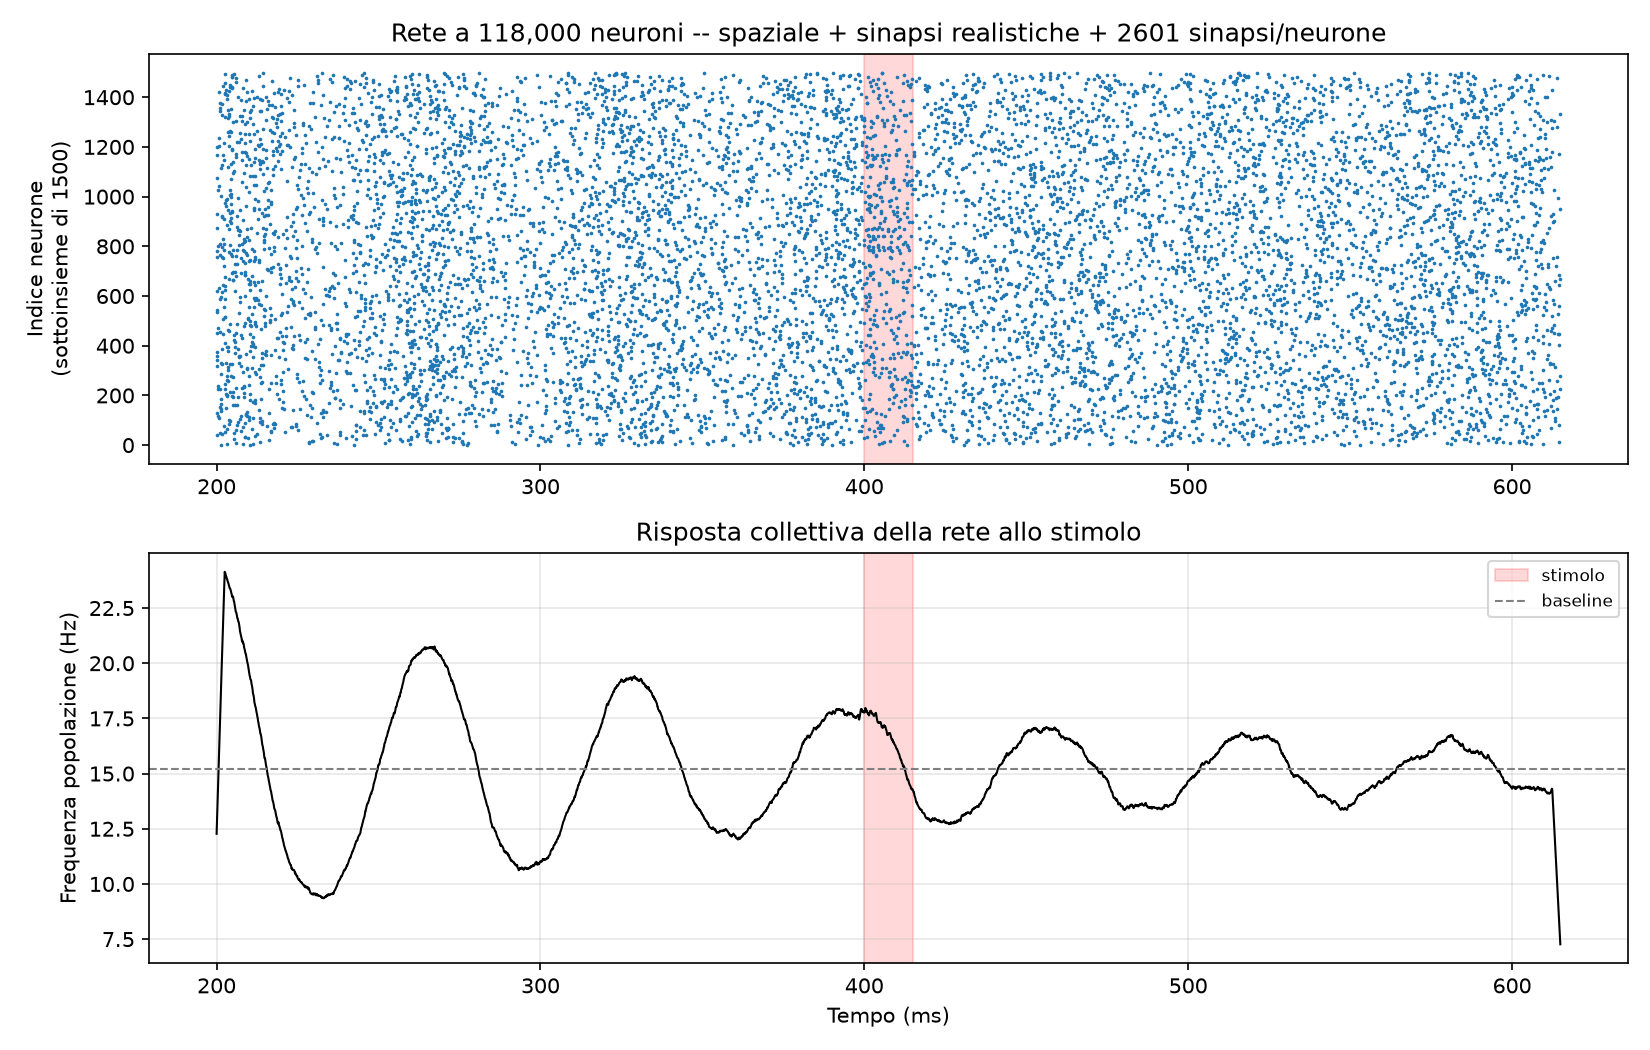
\includegraphics[width=6in,height=3.81818in]{media/media/image19.png}

\emph{Fig. 19 --- Rete finale (118.000 neuroni, spaziale + conduttanza + densita\textquotesingle{} Allen): raster e risposta collettiva, dopo la correzione dei pesi.}

Il grafico rivela un dettaglio qualitativo non catturato dalle sole metriche numeriche: la rete mostra un\textquotesingle oscillazione REGOLARE E PERSISTENTE per tutta la durata della simulazione (periodo di circa 65-70 millisecondi, ampiezza approssimativamente costante), diversa sia dal comportamento instabile del primo tentativo (ampiezza crescente senza limite) sia dal comportamento asincrono irregolare osservato nelle reti piu\textquotesingle{} semplici (sezioni 2.8, 3.6). Lo stimolo (fascia rossa, 400-415ms) cade durante una fase di salita del ciclo naturale della rete, risultando visivamente poco distinguibile dai picchi spontanei adiacenti -\/- un fenomeno che richiederebbe una verifica statistica su piu\textquotesingle{} prove (analoga al PSTH della sezione 2.11) per essere caratterizzato con sicurezza.

\subsection{6.6 Visualizzazione 3D della rete finale}\label{visualizzazione-3d-della-rete-finale}

La rete finale (118.000 neuroni) e\textquotesingle{} stata visualizzata interattivamente esportando le posizioni spaziali e l\textquotesingle attivita\textquotesingle{} nel tempo di un sottoinsieme di 7.867 neuroni (un neurone ogni 15, per mantenere fluida l\textquotesingle animazione nel browser), con gli stessi strumenti sviluppati per le visualizzazioni precedenti (sezione 4.2). Il file HTML risultante e\textquotesingle{} autonomo e interattivo (non incluso come testo in questo documento data la sua natura interattiva, ma allegato separatamente).

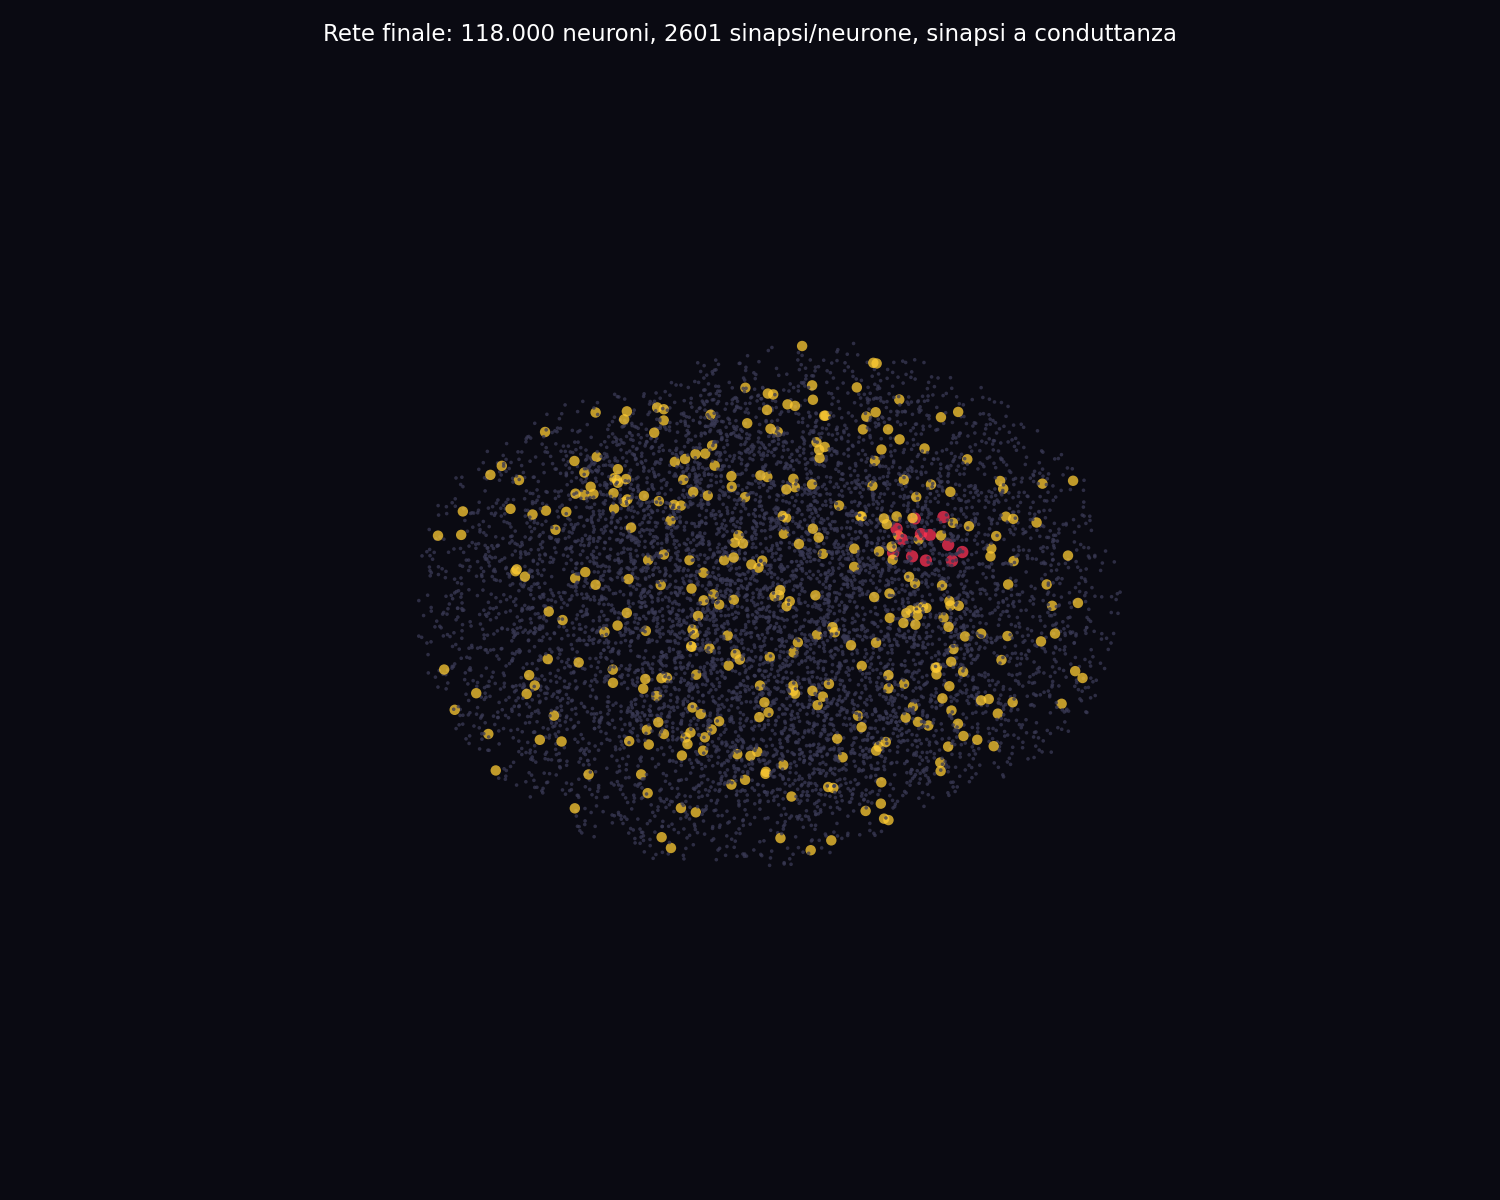
\includegraphics[width=4.3in,height=3.44in]{media/media/image20.png}

\emph{Fig. 20 --- Istantanea della rete finale in 3D (7.867 neuroni renderizzati su 118.000).}

\textit{\textbf{Codice sorgente: rete\_sintesi\_export.py (versione con esportazione dati 3D)}}

\lstinputlisting[language=Python]{scripts/rete_sintesi_export.py}
\subsection{6.7 Confronto finale con l\textquotesingle Allen Institute}\label{confronto-finale-con-lallen-institute}

{\def\LTcaptype{none} % do not increment counter
\begin{longtable}[]{@{}
  >{\raggedright\arraybackslash}p{(\linewidth - 6\tabcolsep) * \real{0.2500}}
  >{\raggedright\arraybackslash}p{(\linewidth - 6\tabcolsep) * \real{0.2500}}
  >{\raggedright\arraybackslash}p{(\linewidth - 6\tabcolsep) * \real{0.2500}}
  >{\raggedright\arraybackslash}p{(\linewidth - 6\tabcolsep) * \real{0.2500}}@{}}
\toprule\noalign{}
\begin{minipage}[b]{\linewidth}\raggedright
\end{minipage} & \begin{minipage}[b]{\linewidth}\raggedright
\textbf{Rete a 40M (scala pura)}
\end{minipage} & \begin{minipage}[b]{\linewidth}\raggedright
\textbf{Rete finale (sintesi)}
\end{minipage} & \begin{minipage}[b]{\linewidth}\raggedright
\textbf{Allen Institute}
\end{minipage} \\
\midrule\noalign{}
\endhead
\bottomrule\noalign{}
\endlastfoot
Neuroni & 40.000.000 & 118.000 & \textasciitilde10.000.000 \\
Sinapsi/neurone & 31 & 2.601 & \textasciitilde2.600 \\
Tipo sinapsi & Salto di tensione & Conduttanza & Conduttanza + morfologia \\
Struttura & Casuale & Spaziale (small-world 3D) & Connettoma reale \\
\% cervello di topo & 57.1\% & 0.169\% & \textasciitilde14.3\% \\
\end{longtable}
}

\textbf{Il confronto finale e\textquotesingle{} onesto su entrambi i fronti: sulla densita\textquotesingle{} sinaptica per neurone, il presente progetto ha raggiunto la PARITA\textquotesingle{} con l\textquotesingle Allen Institute (2.601 contro \textasciitilde2.600); sul numero assoluto di neuroni e sul dettaglio morfologico di ciascuno, il divario resta ampio. Nessuna delle due reti costruite in questo progetto (quella a scala massima e quella a densita\textquotesingle{} massima) domina l\textquotesingle altra su tutti gli assi contemporaneamente -\/- una conseguenza diretta e osservata concretamente del vincolo di memoria condivisa discusso in apertura di questa sezione (6.1).}

\section{7. Discussione}\label{discussione}

\subsection{7.1 Sintesi del percorso completo}\label{sintesi-del-percorso-completo}

Il percorso descritto in questo documento ha permesso di costruire, verificare sperimentalmente e osservare in prima persona una sequenza di sedici fenomeni ed esperimenti neurali di complessita\textquotesingle{} via via crescente, partendo sempre da modelli minimi e aggiungendo un solo elemento di complessita\textquotesingle{} alla volta: comunicazione sinaptica di base, soglia di attivazione, plasticita\textquotesingle{} a breve termine, propagazione in catena, sommazione temporale, apprendimento hebbiano tramite STDP, classificazione elementare di pattern, attivita\textquotesingle{} collettiva bilanciata su una popolazione di 300 neuroni, omeostasi dopo perturbazione, organizzazione modulare, verifica statistica rigorosa, scaling fino a 40 milioni di neuroni, connettivita\textquotesingle{} spaziale strutturata, visualizzazione 3D interattiva, un tentativo fallito e uno riuscito di costruire un attrattore neurale, catene di attrattori collegati, competizione tra alternative, apprendimento per rinforzo, e infine una politica decisionale condizionata al contesto.

Questa sintesi copriva, alla sua prima stesura, solo la prima meta\textquotesingle{} del documento (sezioni 1-5.4). Il percorso e\textquotesingle{} proseguito con un arco distinto ma collegato: comunicazione bidirezionale appresa nel dominio spiking, dal fallimento totale alla soluzione completa (interruttore di trasmissione, normalizzazione omeostatica, soppressione di emergenza -\/- sezioni 5.6-5.17), estesa a piu\textquotesingle{} messaggi simultanei e a una rete a tre popolazioni in staffetta (sezioni 5.18-5.20). Su quella stessa architettura si innesta poi un secondo filone, questa volta di fisica (sezioni 5.21-5.41): l\textquotesingle impatto di fasci ionici clinici del CNAO (Geant4, QBBC) sull\textquotesingle anello neurale, collegato all\textquotesingle architettura spiking tramite un esperimento di knockout funzionale che rivela un gradiente dose-risposta verificato su quattro scenari fisici indipendenti e generalizzato oltre la scelta specifica della dimensione del knockout; un recupero funzionale dopo il danno e un punto di non ritorno quando il danno e\textquotesingle{} completo; un modello RBE clinico (il Microdosimetric Kinetic Model di Kase, lo stesso usato a NIRS/HIMAC a Chiba) implementato e validato contro dati pubblicati prima di essere usato; un limite scoperto e corretto nella riproducibilita\textquotesingle{} della mappa di dose per-neurone; e infine un collegamento nanodosimetrico (Geant4-DNA) verificato end-to-end, dagli elettroni secondari realmente prodotti nei neuroni colpiti fino ai cluster di ionizzazione, coerenti con la letteratura pubblicata. La stessa disciplina metodologica descritta nella sezione 7.2 -\/- verificare empiricamente invece di assumere, documentare i tentativi falliti quanto quelli riusciti -\/- attraversa entrambi i filoni senza soluzione di continuita\textquotesingle.

\subsection{7.2 Le due lezioni metodologiche piu\textquotesingle{} importanti}\label{le-due-lezioni-metodologiche-piu-importanti}

Ripercorrendo l\textquotesingle intero documento, due lezioni metodologiche emergono con particolare chiarezza, ripetute in forme diverse in punti diversi del percorso:

\subsubsection{6.2.1 La differenza tra "sembra vero" e "verificato vero"}\label{la-differenza-tra-sembra-vero-e-verificato-vero}

Almeno tre volte nel corso del progetto, un risultato che appariva convincente a un primo sguardo si e\textquotesingle{} rivelato, dopo verifica statistica rigorosa, non sostenuto dai dati: la propagazione tra moduli nella sezione 2.11 (effetto apparente di +13 Hz, rivelatosi di soli +0.89 Hz una volta mediato su 25 prove indipendenti, ben dentro il rumore di fondo di \textasciitilde4 Hz); il tentativo di persistenza tramite STDP nella sezione 4.3 (attivita\textquotesingle{} apparentemente presente in una singola prova non ripetuta, rivelatasi sistematicamente pari a zero su 16 prove indipendenti correttamente randomizzate); e la rottura di simmetria nella competizione a pesi uguali della sezione 5.2.1 (apparentemente un candidato "vincente" per qualche ragione strutturale, rivelatosi un artefatto numerico deterministico mascherato da rumore insufficiente). In tutti e tre i casi, la differenza tra l\textquotesingle impressione iniziale e il risultato verificato e\textquotesingle{} emersa solo applicando gli strumenti statistici corretti (ripetizione, randomizzazione controllata, confronto con la variabilita\textquotesingle{} naturale del sistema) -\/- non per intuizione o ispezione visiva piu\textquotesingle{} attenta del singolo grafico.

\subsubsection{6.2.2 I tentativi falliti sono parte della conoscenza prodotta, non rumore da nascondere}\label{i-tentativi-falliti-sono-parte-della-conoscenza-prodotta-non-rumore-da-nascondere}

Il tentativo di attrattore tramite STDP (sezione 4.3) e i primi due tentativi di architettura per il ring attractor (sezione 4.4.1, punti 1 e 2) sono falliti in modo completo prima che il terzo tentativo avesse successo. Riportare questi fallimenti nel dettaglio -\/- comprese le ipotesi errate che li motivavano e le ragioni tecniche precise per cui non funzionavano -\/- non e\textquotesingle{} un difetto del documento, ma parte integrante del suo valore: mostra il vero processo con cui si costruisce conoscenza scientifica, che raramente procede in linea retta dal problema alla soluzione.

\subsection{7.3 Cosa manca per una vera funzionalita\textquotesingle{} cerebrale}\label{cosa-manca-per-una-vera-funzionalita-cerebrale}

Anche il risultato piu\textquotesingle{} avanzato del progetto (la politica decisionale contestuale della sezione 5.4) resta a distanza enorme da qualunque cosa si possa onestamente chiamare "funzionalita\textquotesingle{} cerebrale" nel senso pieno del termine. Gli ingredienti mancanti, in ordine approssimativo di difficolta\textquotesingle{} crescente per essere aggiunti:

\begin{itemize}
\item
  Connettivita\textquotesingle{} strutturata reale (un vero connettoma) invece di un modello geometrico semplificato -\/- probabilmente la sfida singola piu\textquotesingle{} grande, tuttora oggetto di ricerca attiva a livello mondiale con i migliori strumenti disponibili (si veda la sezione 4.5)
\item
  Diversita\textquotesingle{} dei tipi cellulari -\/- un cervello reale possiede centinaia di tipi di neurone morfologicamente e funzionalmente distinti, non le due sole categorie omogenee (eccitatorio/inibitorio) usate in questo progetto
\item
  Input sensoriali e output motori strutturati e significativi, provenienti dal mondo reale, invece del rumore casuale di tipo Poisson usato come "attivita\textquotesingle{} di fondo" in tutti gli esperimenti di questo progetto
\item
  Neuromodulazione (dopamina, serotonina, acetilcolina, noradrenalina) che opera su scale di tempo molto piu\textquotesingle{} lente dei singoli impulsi elettrici, regolando dinamicamente la plasticita\textquotesingle{} e l\textquotesingle eccitabilita\textquotesingle{} di intere popolazioni neuronali in funzione dello stato comportamentale
\item
  Sviluppo e apprendimento su scale di tempo di mesi o anni, non i pochi secondi di tempo simulato usati in ogni esperimento di questo progetto
\item
  Generalizzazione a situazioni mai viste prima -\/- la tabella pesi{[}contesto{]}{[}candidato{]} della sezione 5.4 e\textquotesingle{} una memoria associativa (lookup table), non una rappresentazione astratta che permetta di interpolare o generalizzare correttamente a un contesto intermedio mai presentato durante il training
\end{itemize}

\section{8. Limiti del lavoro}\label{limiti-del-lavoro}

\begin{itemize}
\item
  Il modello di Izhikevich e\textquotesingle{} una semplificazione deliberata: non include la morfologia reale del neurone (struttura dendritica, geometria assonale), ne\textquotesingle{} la diversita\textquotesingle{} dei canali ionici presente nei neuroni biologici reali -\/- scelto per necessita\textquotesingle{} di scalare a milioni di neuroni, al costo di un realismo biofisico inferiore rispetto a modelli come Hodgkin-Huxley
\item
  Le connessioni sinaptiche nella maggior parte degli esperimenti sono statiche in peso "istantaneo" (a parte gli esperimenti espliciti di plasticita\textquotesingle, sezioni 2.3, 2.6, 2.7), senza dinamiche di rilascio di neurotrasmettitore realistiche come la depressione a breve termine o la saturazione dei recettori postsinaptici
\item
  L\textquotesingle effetto di propagazione tra moduli (sezioni 2.10-2.11) meriterebbe di essere ritestato con parametri di connettivita\textquotesingle{} inter-modulo piu\textquotesingle{} forti, per capire se un vero effetto emerge in modo piu\textquotesingle{} netto con connessioni piu\textquotesingle{} dense, o se la debolezza osservata a connettivita\textquotesingle{} del 2\% e\textquotesingle{} un risultato robusto che si mantiene anche a connettivita\textquotesingle{} maggiore
\item
  La rete a 40 milioni di neuroni (sezione 3) usa la stessa connettivita\textquotesingle{} casuale a grado fisso delle reti molto piu\textquotesingle{} piccole -\/- un vero avvicinamento strutturale a un cervello di topo richiederebbe di combinare la scala raggiunta con la connettivita\textquotesingle{} spaziale sviluppata separatamente nella sezione 4, cosa che il progetto non ha avuto il tempo di realizzare congiuntamente alla scala massima
\item
  Il rallentamento da throttling termico (sezione 3.4) introduce una variabile hardware non completamente controllata negli esperimenti piu\textquotesingle{} lunghi, rendendo le stime di tempo per esperimenti futuri di scala paragonabile intrinsecamente incerte
\item
  Il bias sistematico di posizione (\textasciitilde0.045 unita\textquotesingle) osservato ripetutamente negli esperimenti con il ring attractor (sezioni 4.4.2, 5.1, 5.2) non e\textquotesingle{} stato completamente diagnosticato alla radice -\/- probabilmente un artefatto di discretizzazione della griglia a N=200 punti, ma senza una verifica formale che lo escluda come effetto reale del modello
\item
  La politica contestuale della sezione 5.4 e\textquotesingle{} stata verificata solo su 3 contesti discreti e ben separati sull\textquotesingle anello -\/- non e\textquotesingle{} stato testato se il meccanismo generalizza a un numero maggiore di contesti, a contesti piu\textquotesingle{} ravvicinati spazialmente (che potrebbero interferire tra loro), o alla capacita\textquotesingle{} di interpolare correttamente per un contesto intermedio mai presentato durante il training
\item
  Nessuno degli esperimenti di questo progetto include una fase di validazione incrociata o un insieme di test completamente separato dal training -\/- una pratica standard in machine learning per escludere l\textquotesingle overfitting, che non e\textquotesingle{} stata applicata sistematicamente data la natura esplorativa del lavoro
\end{itemize}

I limiti sopra riguardano il filone di neuroscienza pura (sezioni 1-5.20). Il filone di fisica collegato (Geant4/CNAO/Chiba, sezioni 5.21-5.41) ha i propri, distinti: la mappa di dose per-neurone e\textquotesingle{} fondamentalmente limitata dalla statistica di conteggio (ogni neurone, 10um di raggio, intercetta in media solo 1-2 primari diretti su 500.000 eventi simulati -\/- un limite quantificato nella sezione 5.37, non risolvibile con un fattore 10 di statistica in piu\textquotesingle, verosimilmente servirebbe un fattore 100-1000, computazionalmente proibitivo con la fisica adronica completa di QBBC nei tempi di questo progetto).

Il modello RBE (sezione 5.34) e\textquotesingle{} il vero Microdosimetric Kinetic Model di Kase, non piu\textquotesingle{} un\textquotesingle approssimazione ad hoc, ma resta semplificato rispetto al modello clinico completo su due punti dichiarati: usa il LET dose-mediato come proxy della dose-mean lineal energy (che richiederebbe uno spettro misurato con un TEPC o una vera simulazione microdosimetrica di sito), e calcola la correzione di saturazione nel limite a valore singolo invece che integrando uno spettro completo.

Il knockout funzionale (sezioni 5.22-5.38) resta un modello deliberatamente semplificato del danno neuronale -\/- rimozione completa delle sinapsi in uscita sopra una soglia di dose relativa, non un modello di danno biologico validato (nessuna soglia assoluta di dose per l\textquotesingle inattivazione di un singolo neurone e\textquotesingle{} consolidata in letteratura, lo stesso limite dichiarato nel paper Villagrasa/Baiocco che il progetto gemello geant4dna\_icsd riproduce).

Il collegamento nanodosimetrico (sezioni 5.39-5.41) si ferma al livello degli ICSD (Ionization Cluster Size Distribution) -\/- non modella il danno al DNA (rotture singole o doppie, SSB/DSB), che richiederebbe un modello geometrico di nucleo cellulare con cromatina multi-scala (disponibile in Geant4-DNA, es. gli esempi ufficiali dnadamage1/molecularDNA, ma non integrato qui).

\section{9. Possibili sviluppi futuri}\label{possibili-sviluppi-futuri}

\begin{itemize}
\item
  Combinare la scala raggiunta (sezione 3, 40 milioni di neuroni) con la connettivita\textquotesingle{} spaziale sviluppata separatamente (sezione 4), per ottenere una rete contemporaneamente grande E strutturata -\/- il passo naturale successivo per avvicinarsi ulteriormente a un vero cervello di topo su entrambi gli assi di realismo
\item
  Rendere plastiche (STDP) anche le connessioni tra i due ring attractor della sezione 5.1, per studiare se e come l\textquotesingle offset della mappa associativa possa essere esso stesso APPRESO dal sistema invece di essere fissato a priori dall\textquotesingle esterno
\item
  Ripetere la verifica statistica rigorosa (tecnica PSTH, sezione 2.11) anche sugli esperimenti di attrattore e apprendimento per rinforzo delle sezioni 4 e 5, per verificare la robustezza statistica dei risultati positivi ottenuti su un numero relativamente limitato di prove (6-18 a seconda dell\textquotesingle esperimento)
\item
  Estendere la politica contestuale (sezione 5.4) a un numero maggiore di contesti, e testare esplicitamente la capacita\textquotesingle{} di generalizzazione a contesti intermedi mai visti durante il training -\/- il vero banco di prova per distinguere una memoria associativa pura da un inizio di rappresentazione astratta
\item
  Esplorare una topologia di rete a piu\textquotesingle{} di due moduli (sezione 2.10), con pattern di connettivita\textquotesingle{} ispirati a reali mappe di connettivita\textquotesingle{} corticale pubblicate (ad esempio quelle dell\textquotesingle Allen Institute, sezione 4.5.2), invece del kernel geometrico artificiale usato in questo progetto
\item
  Testare l\textquotesingle accesso a un cluster di calcolo universitario (ad esempio tramite il CNAO o il Dipartimento di Fisica dell\textquotesingle Universita\textquotesingle{} di Pavia) per superare il limite di RAM di un laptop personale, verificato empiricamente nella sezione 3.3 attorno ai 40-50 milioni di neuroni con connettivita\textquotesingle{} casuale semplice
\item
  Investigare formalmente l\textquotesingle origine del bias sistematico di posizione osservato nel ring attractor (sezioni 4.4.2, 5.1, 5.2), per determinare se sia un artefatto puramente numerico o rifletta una proprieta\textquotesingle{} reale (per quanto non desiderata) del modello discretizzato
\end{itemize}

Gli sviluppi futuri sopra riguardano il filone di neuroscienza pura. Per il filone di fisica (Geant4/CNAO/Chiba), i punti aperti restano quelli del progetto gemello geant4dna\_icsd (vedi il suo README): implementare il dataset di sezioni d\textquotesingle urto "comuni" definito nel paper Villagrasa/Baiocco (richiede estrarre i valori numerici dal materiale supplementare e scrivere una sottoclasse G4VEmModel dedicata -\/- un lavoro sostanziale, non un\textquotesingle estensione da weekend, come il paper stesso segnala) e, soprattutto, estendere la catena fisica gia\textquotesingle{} verificata (dose macroscopica -\textgreater{} spettro di elettroni secondari -\textgreater{} ICSD nanodosimetrico) fino al danno al DNA (SSB/DSB) con un modello geometrico di nucleo cellulare -\/- il passo naturale successivo per rendere il collegamento clinicamente interpretabile, non solo fisicamente coerente. \emph{{[}Aggiornamento: il danno SSB/DSB e\textquotesingle{} stato completato nella sezione 5.42, con l\textquotesingle esempio moleculardna invece di dnadamage1/molecularDNA (bloccato da una dipendenza esterna mancante) -\/- resta aperto solo il dataset di sezioni d\textquotesingle urto comuni del paper.{]}}

\section{10. Glossario dei termini tecnici usati nel documento}\label{glossario-dei-termini-tecnici-usati-nel-documento}

\textbf{Attrattore:} Uno stato (o insieme di stati) verso cui un sistema dinamico converge nel tempo, e a cui ritorna dopo piccole perturbazioni. Il ring attractor della sezione 4.4 e\textquotesingle{} l\textquotesingle esempio concreto costruito in questo progetto.

\textbf{Bandito multi-braccio (multi-armed bandit):} Un problema classico di reinforcement learning in cui un agente deve scegliere ripetutamente tra piu\textquotesingle{} alternative ("braccia"), ciascuna con una ricompensa media diversa e sconosciuta, imparando quale scegliere piu\textquotesingle{} spesso tramite tentativi ripetuti.

\textbf{Bilanciamento eccitazione-inibizione (E/I balance):} Il rapporto e l\textquotesingle equilibrio dinamico tra neuroni eccitatori (che spingono altri neuroni verso lo spike) e inibitori (che li sopprimono) in una rete, necessario per ottenere attivita\textquotesingle{} stabile invece di esplosione o silenzio.

\textbf{Brian2:} Libreria Python per la simulazione di reti neurali a impulsi (spiking), usata per tutti gli esperimenti spiking di questo progetto.

\textbf{Bump attractor:} Un tipo specifico di attrattore neurale in cui lo stato stabile e\textquotesingle{} una regione localizzata di attivita\textquotesingle{} elevata ("il bump") su un substrato spaziale piu\textquotesingle{} ampio, tipicamente un anello o una griglia. Vedi sezione 4.4.

\textbf{Connettoma:} La mappa completa delle connessioni sinaptiche tra tutti i neuroni di un sistema nervoso (o di una sua porzione).

\textbf{Deviazione standard:} Una misura statistica della dispersione di un insieme di valori attorno alla loro media -\/- usata ripetutamente in questo documento per distinguere un vero effetto dal rumore casuale.

\textbf{Izhikevich (modello di):} Modello matematico del neurone a due equazioni differenziali accoppiate, proposto da Eugene Izhikevich nel 2003. Vedi sezione 1.2.

\textbf{KD-tree:} Struttura dati che organizza punti in uno spazio K-dimensionale per permettere ricerche di vicinato spaziale efficienti, usata nella sezione 4.2 per calcolare la connettivita\textquotesingle{} spaziale di reti fino a 1 milione di neuroni.

\textbf{Omeostasi:} La capacita\textquotesingle{} di un sistema di tornare a uno stato di equilibrio stabile dopo una perturbazione, senza intervento esterno. Osservata per la prima volta nella sezione 2.9.

\textbf{PSTH (Peristimulus Time Histogram):} Tecnica statistica standard in neuroscienza sperimentale per misurare la risposta media di un sistema a uno stimolo, mediando su molte ripetizioni indipendenti allineate rispetto al momento dello stimolo. Vedi sezione 2.11.

\textbf{Rescorla-Wagner (regola di):} Modello matematico storico (1972) dell\textquotesingle apprendimento associativo, in cui la forza di un\textquotesingle associazione viene aggiornata proporzionalmente alla differenza tra la ricompensa ricevuta e quella attesa. Usata come base della regola di aggiornamento nella sezione 5.3.

\textbf{Ring attractor:} Un attrattore neurale implementato su una topologia ad anello, dove la posizione del bump codifica una variabile continua (ad esempio una posizione spaziale o un orientamento). Vedi sezione 4.4.

\textbf{Small-world (topologia):} Un pattern di organizzazione di rete caratterizzato da connessioni dense e locali combinate con rare connessioni a lunga distanza, osservato in moltissimi sistemi biologici e sociali reali. Proposto da Watts e Strogatz nel 1998. Vedi sezione 4.1.

\textbf{Spike / potenziale d\textquotesingle azione:} L\textquotesingle impulso elettrico che un neurone genera quando il suo potenziale di membrana supera una soglia, il meccanismo fondamentale di comunicazione tra neuroni.

\textbf{STDP (Spike-Timing-Dependent Plasticity):} Regola di apprendimento sinaptico in cui il rafforzamento o indebolimento di una sinapsi dipende dall\textquotesingle ordine temporale preciso tra gli spike del neurone presinaptico e postsinaptico. Vedi sezione 2.6.

\textbf{Winner-take-all:} Un meccanismo computazionale, tipicamente implementato tramite inibizione globale o laterale, in cui solo un elemento (o un piccolo sottoinsieme) di un sistema competitivo puo\textquotesingle{} restare attivo, sopprimendo tutti gli altri candidati.

\section{11. Materiali e riproducibilita\textquotesingle{}}\label{materiali-e-riproducibilita}

Tutti gli script Python sviluppati durante il progetto sono stati verificati eseguendoli realmente (non solo scritti) e sono pienamente riproducibili. Il codice sorgente completo o quasi completo di ciascuno script principale e\textquotesingle{} incluso nel corpo di questo documento, nella sezione corrispondente; l\textquotesingle elenco seguente li riepiloga con un riferimento alla sezione dove sono discussi.

{\def\LTcaptype{none} % do not increment counter
\begin{longtable}[]{@{}
  >{\raggedright\arraybackslash}p{(\linewidth - 4\tabcolsep) * \real{0.3333}}
  >{\raggedright\arraybackslash}p{(\linewidth - 4\tabcolsep) * \real{0.3333}}
  >{\raggedright\arraybackslash}p{(\linewidth - 4\tabcolsep) * \real{0.3333}}@{}}
\toprule\noalign{}
\begin{minipage}[b]{\linewidth}\raggedright
\textbf{File}
\end{minipage} & \begin{minipage}[b]{\linewidth}\raggedright
\textbf{Sezione}
\end{minipage} & \begin{minipage}[b]{\linewidth}\raggedright
\textbf{Contenuto}
\end{minipage} \\
\midrule\noalign{}
\endhead
\bottomrule\noalign{}
\endlastfoot
due\_neuroni.py & 2.1 & Comunicazione base tra due neuroni \\
esplorazione\_parametri.py & 2.2 & Soglia sinaptica \\
plasticita\_sinaptica.py & 2.3 & Facilitazione a breve termine \\
rete\_catena.py & 2.4 & Propagazione in catena \\
rete\_convergente.py & 2.5 & Sommazione temporale \\
stdp.py & 2.6 & Spike-Timing-Dependent Plasticity \\
classificazione\_stdp.py & 2.7 & Apprendimento selettivo di pattern \\
rete\_300\_neuroni.py & 2.8 & Rete bilanciata E/I \\
rete\_300\_stimolo.py & 2.9 & Risposta a stimolo e recovery \\
due\_moduli.py & 2.10 & Architettura modulare \\
psth\_moduli.py & 2.11 & Verifica statistica su 25 prove \\
scaling\_verso\_topo.py, scaling\_fase2/3/4.py & 3.5 & Scaling progressivo automatico \\
rete\_40M\_finale.py & 3.6 & Esperimento finale a 40 milioni di neuroni \\
rete\_smallworld.py & 4.1 & Connettivita\textquotesingle{} small-world su anello \\
brain3d\_visualization.html, brain1M\_visualization.html & 4.2 & Visualizzazioni 3D interattive \\
ring\_attractor\_rate.py & 4.4 & Ring attractor, risultato finale verificato \\
chained\_attractors.py & 5.1 & Catena di due attrattori collegati \\
competing\_targets.py & 5.2 & Competizione tra alternative \\
rl\_bandit.py & 5.3 & Apprendimento per rinforzo (bandito) \\
contextual\_policy.py & 5.4 & Politica decisionale contestuale \\
rete\_sintesi\_export.py & 6.4-6.6 & Sintesi finale: spaziale + conduttanza + densita\textquotesingle{} Allen \\
dialogo\_ring\_attractor.py & 5.5.1 & Scambio a turni tra due ring, canali fissi \\
dialogo\_stdp.py & 5.5.2 & Sinapsi A-\textgreater B appresa (Hebbiano a grana di turno); asimmetria B-\textgreater A documentata \\
dialogo\_stdp\_adattamento.py & 5.5.3 & Adattamento + riscaldamento: entrambi i canali affidabili al 100\% \\
dialogo\_multi\_messaggio.py & 5.5.4 & Piu\textquotesingle{} messaggi sulla stessa sinapsi: test di interferenza \\
dialogo\_multi\_normalizzato.py & 5.5.5 & Normalizzazione omeostatica su W\_AB: competizione resa visibile, non risolta \\
dialogo\_multi\_repulsione.py & 5.5.6 & Esplorazione repulsiva: interferenza risolta, 7 scambi su 8 al 100\% \\
diagnosi\_bias\_posizione.py & 5.5.7 & Verifica diretta (e smentita) dell\textquotesingle ipotesi del bias di posizione \\
dialogo\_multi\_repulsione\_3msg.py & 5.5.8 & Scalabilita\textquotesingle{} a 3 messaggi: separazione migliore, consolidamento peggiore (risultato aperto) \\
dialogo\_multi\_scoperta\_locale.py & 5.5.9 & Repulsione solo per la scoperta + esplorazione locale: 10/12 scambi, miglior risultato \\
dialogo\_multi\_scoperta\_locale\_montecarlo.py & 5.5.10 & Verifica Monte Carlo (8 seed): 91.7\% di successo, ma l\textquotesingle ipotesi sul residuo era sbagliata \\
dialogo\_multi\_scoperta\_locale\_permutazione.py & 5.5.11 & Disambiguazione posizione/valore: turno 5 segue l\textquotesingle ordine, turno 7 segue il valore \\
dialogo\_multi\_scoperta\_locale\_mischiato.py & 5.5.12 & Ordine del round-robin mescolato: piu\textquotesingle{} equo tra i messaggi, ma tasso aggregato piu\textquotesingle{} basso (87.5\% vs 91.7\%) \\
dialogo\_multi\_scoperta\_bidirezionale.py & 5.5.13 & Scoperta+consolidamento locale su entrambi i canali: 95.8\%, turno 7 risolto al 100\% \\
ring\_attractor\_spiking.py & 5.6 & Primo ring attractor spiking stabile (10 tentativi di tuning, sinapsi NMDA-like) \\
dialogo\_spiking.py & 5.7 & Comunicazione appresa A-\textgreater B tra due ring attractor spiking, STDP vera \\
dialogo\_spiking\_bidirezionale.py & 5.8 & Tentativo di bidirezionalita\textquotesingle{} spiking: stessa asimmetria del modello a rate, non risolta \\
dialogo\_spiking\_bidirezionale\_turni.py & 5.9 & Schema a turni A/B per isolare il confondimento nel canale B-\textgreater A spiking \\
dialogo\_spiking\_bidirezionale\_gate.py & 5.9 & Plasticita\textquotesingle{} B-\textgreater A confinata ai turni non confusi: conclusione negativa definitiva \\
dialogo\_spiking\_multi.py & 5.10 & Due messaggi in dominio spiking, STDP vera: nessuna interferenza \\
dialogo\_spiking\_multi\_montecarlo.py & 5.11 & Verifica Monte Carlo (8 seed): nessuna interferenza spiking confermata 16/16 \\
diagnosi\_sottosoglia\_ba.py & 5.12 & Verifica sotto-soglia del canale B-\textgreater A: confusa dalla dinamica propria di A \\
diagnosi\_ablazione\_ba.py & 5.12 & Ablazione: canale B-\textgreater A forte causa esplosione numerica, non segnale causale \\
dialogo\_spiking\_bidirezionale\_silenzia.py & 5.12 & Silenziamento attivo di A: stessa esplosione, conclusione finale \\
dialogo\_spiking\_bidirezionale\_interruttore.py & 5.13 & Interruttore di trasmissione: stabile con pesi bassi, un seed su quattro \\
diagnosi\_unidirezionale\_pesi\_forti.py & 5.13 & Controllo: canale unidirezionale con pesi forti e\textquotesingle{} stabile da solo \\
dialogo\_spiking\_bidirezionale\_interruttore\_mc.py & 5.13 & Verifica Monte Carlo (4 seed): solo 1/4 stabile, la \textquotesingle vittoria\textquotesingle{} era un caso fortunato \\
dialogo\_spiking\_bidirezionale\_omeostasi.py & 5.14 & Normalizzazione omeostatica dei pesi: bidirezionalita\textquotesingle{} spiking stabile sul seed di base \\
dialogo\_spiking\_bidirezionale\_omeostasi\_mc.py & 5.14 & Verifica Monte Carlo (8 seed): 6/8 stabili, miglioramento reale ma non completo \\
dialogo\_spiking\_bidirezionale\_omeostasi\_v2.py & 5.15 & Omeostasi piu\textquotesingle{} reattiva: crescita bidirezionale pulita sul seed di base \\
dialogo\_spiking\_bidirezionale\_omeostasi\_v2\_mc.py & 5.15 & Verifica Monte Carlo (8 seed): 7/8 stabili, migliore di v1 \\
diagnosi\_seed301\_anello\_isolato.py & 5.16 & Verifica: anello isolato del seed 301 e\textquotesingle{} stabile da solo \\
dialogo\_spiking\_bidirezionale\_omeostasi\_v3.py & 5.16 & Interruttore di emergenza sopra l\textquotesingle omeostasi graduale \\
dialogo\_spiking\_bidirezionale\_omeostasi\_v3\_mc.py & 5.16 & Verifica Monte Carlo (8 seed): 7/8 puliti, ottavo migliorato 40x \\
dialogo\_spiking\_bidirezionale\_omeostasi\_v4.py & 5.17 & Bidirezionalita\textquotesingle{} spiking risolta: interruttore trasmissione + omeostasi + soppressione diretta \\
dialogo\_spiking\_bidirezionale\_omeostasi\_v4\_mc.py & 5.17 & Verifica Monte Carlo (8 seed): 8/8 stabili, crescita bidirezionale in ogni run \\
dialogo\_spiking\_bidirezionale\_multi.py & 5.18 & Piu\textquotesingle{} messaggi bidirezionali spiking: completamento del filone \\
dialogo\_spiking\_bidirezionale\_multi\_mc.py & 5.18 & Verifica Monte Carlo (8 seed): 8/8 stabili, nessuna interferenza \\
dialogo\_spiking\_bidirezionale\_multi3.py & 5.19 & Tre messaggi bidirezionali spiking: stress-test del carico \\
dialogo\_spiking\_bidirezionale\_multi3\_mc.py & 5.19 & Verifica Monte Carlo (8 seed): 8/8 stabili, 98\% localizzazione sotto soglia \\
dialogo\_spiking\_relay\_3anelli.py & 5.20 & Staffetta a tre popolazioni A-\textgreater B-\textgreater C-\textgreater A, primo passo oltre la coppia \\
dialogo\_spiking\_relay\_3anelli\_mc.py & 5.20 & Verifica Monte Carlo (6 seed): informazione preservata su due salti in ogni caso \\
dialogo\_spiking\_cnao\_knockout.py & 5.22 & Knockout dei neuroni a dose CNAO piu\textquotesingle{} alta: interrompe selettivamente il messaggio che li usa \\
dialogo\_spiking\_cnao\_knockout\_mc.py & 5.23 & Verifica Monte Carlo (8 seed): knockout robusto, 8/8 stessa direzione \\
dialogo\_spiking\_knockout\_controllo\_mc.py & 5.24 & Controllo negativo: knockout casuale non riproduce l\textquotesingle effetto selettivo \\
braggProfile/braggProfile.cc & 5.25 & Profilo di dose in profondita\textquotesingle: trova il picco di Bragg, scopre un artefatto geometrico in cnaoRingImpact \\
dialogo\_spiking\_cnao\_knockout\_v2\_mc.py & 5.26 & Ri-verifica con dose corretta: l\textquotesingle effetto si ribalta come previsto (test falsificabile superato) \\
dialogo\_spiking\_cnao\_knockout\_picco\_mc.py & 5.27 & Dataset completo al picco + gradiente dose-risposta su tre livelli di sovrapposizione \\
dialogo\_spiking\_cnao\_knockout\_proton\_mc.py & 5.28 & Knockout con mappa di dose da protoni: effetto piu\textquotesingle{} forte finora (7.07x, 8/8), gradiente a 4 punti completo \\
dialogo\_spiking\_cnao\_recupero.py & 5.29 & Recupero funzionale dopo il knockout: la plasticita\textquotesingle{} residua compensa progressivamente, verificato su 4 seed \\
dialogo\_spiking\_lesione\_completa\_mc.py & 5.30 & Lesione completa della zona di codifica: il recupero visto in 5.29 sparisce, punto di non ritorno confermato su 5 run (1+4 MC) \\
geant4\_cnao\_ring (RunAction.cc + analisi RBE) & 5.31 & Modello RBE-LET (Kanai/NIRS): il gradiente 5.22-5.28 regge entro la stessa profondita\textquotesingle; scoperta variabilita\textquotesingle{} Monte Carlo tra run fisici non ancora verificata \\
geant4\_cnao\_ring (cnaoRingImpact.cc, seed esplicito) & 5.32 & Scoperto: la mappa di dose per-neurone e\textquotesingle{} dominata dal rumore Monte Carlo (overlap 1.0/10 su 4 seed); il meccanismo causale neuroscientifico resta valido, la corrispondenza a livello di singolo neurone no \\
dialogo\_spiking\_cnao\_knockout\_media4seed\_mc.py & 5.33 & Knockout da dose mediata su 4 seed Geant4: overlap 1-vs-0 indistinguibile dal controllo negativo, emerge una soglia minima di sbilanciamento (\textasciitilde2 neuroni) per un effetto reale \\
geant4\_cnao\_ring/analysis/mkm\_rbe.py & 5.34 & Modello MKM reale di Kase/NIRS (non piu\textquotesingle{} l\textquotesingle approssimazione lineare della 5.31), validato contro dati pubblicati entro il 10-15\%; conferma la 5.31 con un modello clinico vero \\
geant4\_cnao\_ring/analysis/mkm\_rbe.py (dataset completo) & 5.35 & MKM su tutte e sei le configurazioni CNAO: overlap fisica/biologica 9-10/10 ovunque; overkill del carbonio e RBE anomalo del protone a 150 MeV \\
geant4\_cnao\_ring/src/SteppingAction.cc (diagnostica CNAO\_DEBUG\_NEURON) & 5.36 & Verificato empiricamente (non solo ipotizzato) il picco di LET anomalo della 5.35: e\textquotesingle{} il protone primario quasi fermo (range straggling), non un frammento secondario -\/- collegato al dibattito reale sull\textquotesingle RBE variabile al bordo distale in protonterapia \\
build/results\_highstat/ (carbonio 5M eventi, seed 501/502) & 5.37 & Quantificato: 10x eventi migliora la sovrapposizione da 1.0/10 (puro rumore) a 2/10 -\/- non basta; confermato che mediare su seed (5.33) e\textquotesingle{} piu\textquotesingle{} efficiente che aumentare gli eventi \\
dialogo\_spiking\_cnao\_knockout\_top5\_mc.py / top20\_mc.py & 5.38 & La dimensione del knockout (5, 10, 20 neuroni) non e\textquotesingle{} speciale: TOP-5 (overlap 0-vs-0) nullo come previsto, TOP-20 (overlap invertito) inverte l\textquotesingle effetto (1.74x, 7/8) esattamente come previsto \\
geant4\_cnao\_ring (DetectorConstruction.cc, taglio di produzione) & 5.39 & Primo passo del collegamento nanodosimetrico: scoperto e corretto un bug (taglio di produzione troppo grosso), spettro reale degli elettroni secondari verificato (100\% sotto 1 MeV, mediana 1.86 keV) -\/- il presupposto fisico dell\textquotesingle accoppiamento con Geant4-DNA e\textquotesingle{} confermato \\
geant4dna\_icsd/build/nanoICSD (energie reali dalla 5.39) & 5.40 & Collegamento nanodosimetrico completato: ICSD da energie di elettroni secondari REALI (CNAO) si inseriscono coerentemente tra i punti gia\textquotesingle{} pubblicati nel paper Villagrasa/Baiocco -\/- catena macro-a-nano verificata end-to-end \\
geant4dna\_icsd/nanoICSD.cc (seed esplicito, verifica 4 seed) & 5.41 & Verifica Monte Carlo di nanoICSD: M1=1.090 confermato stabile (CV 0.34\% su 4 seed) -\/- a differenza della mappa di dose (5.32), qui non c\textquotesingle e\textquotesingle{} un problema di rumore statistico \\
geant4dna\_ssbdsb (moleculardna, energie reali dalla 5.39) & 5.42 & Danno DNA reale (SSB/DSB) da elettroni secondari CNAO: frazione DSB piu\textquotesingle{} alta a bassa energia (LET piu\textquotesingle{} alto), verificato su 3 seed (SB CV 1.8\%, DSB CV 12.4\%) -\/- chiude il collegamento nanodosimetrico fino al livello del DNA \\
geant4dna\_ssbdsb/results/spectrum\_weighted (6 punti pesati) & 5.43 & Danno DNA pesato sull\textquotesingle intero spettro reale (6 punti, non 2): frazione DSB monotona con l\textquotesingle energia (15.7\% a 5.4\%), media pesata finale 9.5\% -\/- chiude l\textquotesingle ultimo limite dichiarato nella 5.42 \\
geant4\_cnao\_ring (tracking DSB per-neurone) & 5.44 & Ponte fisica-neuroscienza chiuso fino al DNA: classifica a danno DSB stimato per-neurone sovrapposta 9/10 con quella a dose fisica -\/- la dose fisica resta un criterio robusto anche al livello di realismo biologico piu\textquotesingle{} profondo raggiunto \\
\end{longtable}
}

\emph{Ambiente di esecuzione: Python 3.14, Brian2 2.10.1, NumPy, SciPy, Matplotlib, su MacBook Air con chip Apple M5 e 24 GB di RAM. Le due visualizzazioni interattive 3D richiedono un browser web moderno con supporto WebGL (Chrome, Safari, Firefox in versioni recenti) e sono autonome (i dati della simulazione sono incorporati direttamente nel file HTML, non richiedono connessione a internet salvo il caricamento iniziale della libreria Three.js da CDN).}

\emph{Fine del documento.}

\end{document}
